\documentclass[10pt,twoside]{report}

\section*{Abstract}

The theoretical understanding behind the principles of quantum mechanics is just the first step towards solving quantum problems in real-world scenarios. Recently, a promising new field has emerged at the intersection of quantum variational methods and machine learning. This approach, named Neural Quantum States, takes advantage of neural networks as universal approximators to efficiently parametrise quantum systems.

This thesis explores the intersection of quantum many-body problems and machine learning, focussing on the application of neural network architectures to solve challenging quantum systems. We specifically investigate three methods: a standard variational Monte Carlo (VMC) parametrisation, a restricted Boltzmann machine (RBM), and a Deep Set feed-forward network (DSFFN). We applied these ansätze to two bound fermionic systems: a one-dimensional polarised fermionic system with Gaussian finite-range interaction, up to six particles and a two-dimensional quantum dots system with Coulomb interaction, up to 20 particles. The study employs Slater-Jastrow variants for the ansätze to impose fermionic antisymmetry, correlations, and cusp conditions. We experimented with various machine learning optimisation techniques, including an extensive Bayesian hyperparameter search, several well-known machine learning optimisers, and a stochastic reconfiguration, a quantum analogue of the natural gradient optimiser, known for its advantage in capturing the geometry of the quantum landscape.

Our implementation is based on Python, aiming at building a modern, modular framework with reasonable efficiency provided by using JAX as back-end. We compare the performance of these methods, discussing their strengths and limitations in representing quantum states efficiently. Our computational efficiency evaluation revealed reasonable scalability with JAX as back-end, though not matching C++ implementations as expected.

We successfully obtained ground-state energies, energy components, density profiles, and correlation energies for quantum systems replicating the results of other research studies with occasional better accuracy. Our results for 1D systems consistently surpassed Hartree-Fock and matched small-basis CI calculations. For 2D quantum dots, the addition of correlation factors repeatedly yielded lower energies than Hartree-Fock, approaching DMC calculations and even surpassing them in one instance using Stochastic Reconfiguration. We addressed the challenges of training neural networks in this unsupervised manner, highlighting the importance of reference energy values and correlation factors. Although more expressive models such as DSFFN showed excellent results, they were harder to train, requiring a balance between model complexity and user intuition. 



\newpage
\section*{Acknowledgements}

This thesis is what brought me to Oslo, but my friends are the reason I stay. I dedicate this work to all my friends and family. To those who started to love me because I came into their life and those who did not stop despite me leaving. None of this would be possible without the support of my family. None of this would be pleasant without the presence of my friends.

I would especially like to thank my supervisor, Morten Hjorth-Jensen, for all the guidance and support. Your enthusiasm and trust in whatever path I wanted to explore kept me motivated from the first day of this project onwards.

A special thank you to Nigar Abbasova, Adam Jakobsen, and Leah Hansen, for being the best second family I could have asked for. To Anna Aasen and Jonny Aarstad Igeh for taking me into the group and making me feel like I belonged somewhere, and to Hkon Kvernmoen, who, on top of that, endured my non-sensical questions about quantum mechanics, convincing me they were in fact not trivial. Finally, to everyone at CCSE: office mates, lunch companies, and table tennis rivals, thank you.

\begin{document}
	
	%Quantum Mechanical Studies of Infinite Matter, with an Emphasis on Nuclear Matter, Neutron Star Matter, and Neutrino Spectra
	%Quantum Mechanical Studies of Infinite Nuclear Matter, by use of Pionless Chiral Potentials
	%{\huge\bfseries Quantum Mechanical Studies of Infinite Nuclear Matter, by use of Chiral Effective Lagrangians\par}
	
	\begin{titlepage}
		\centering
		\vspace{3cm}
		%{\scshape\Large Master Thesis\par}
		\vspace{1.5cm}
		{\huge\bfseries Quantum Mechanical Studies of Infinite Matter by the use of Coupled-Cluster Calculations, with an Emphasis on Nuclear Matter\par}
		\vspace{2cm}
		{\Large\itshape Sean Bruce Sangolt Miller\par}
		\vfill
		\includegraphics*[scale=0.2]{posliten.png}
		\vfill
		{\scshape\large Thesis submitted for the degree of \\ 
			 Master of Science \\ in Subatomic Physics \par}
		\vfill
		{\scshape\LARGE University of Oslo \par}
		{\scshape\large Faculty of Mathematics and Natural Sciences \par}
		{\scshape\large Department of Physics \par}
		
		%\vfill
		\vspace{0.5cm}
		
		% Bottom of the page
		{\large \scshape May, 2017 \par}
	\end{titlepage}
	
	\chapter*{Acknowledgements}
	
	Now, at the end of writing my Master thesis, I have many people to thank for helping me achieve what is contained within these pages. Of the many people I should thank, I have a few I would like to mention in particular:\\
	
	Professor Morten Hjorth-Jensen, for your advisement and guidance for this project, as well as the wealth of insight into nuclear systems. You have made a very difficult field to learn much clearer to me, and helped me make something I am proud of. \\
	
	Audun Skau Hansen, for all the meetings on the practical aspects of performing a coupled-cluster analysis. Without your guidance and great teaching, I would not have been able to do half of the analyses done here.\\
	
	I would like to thank the Computational Physics group for my office space. It might not sound very appreciative, so perhaps I should divulge. My office space has allowed me to get in touch with my fellow students, many of whom have given me countless advice on both my work and other things not quite related to work (like food, games, and other key aspects of life). You have changed my views on many things while I have been here, and I believe it has made me much more open-minded and dedicated. I have been given a superb work space with many resources. The coffee has also been top notch.\\
	
	I would like thank my good friends Filip Henrik Larsen and Roar Emaus. When I took my place here at the Computational Physics department, I do not mind admitting I was a little scared. My interests up to that point had been purely theoretical, and delving into numerical implementation, with as little experience as I had, seemed difficult. Filip and Roar helped me  a great deal in ridding me of my fears and made my time here much better.\\
	
	I want to thank my family for well just about everything. I find it difficult to put into words what I am thankful for. You have supported me, given me advice, taught me all that I hold important in life, told me (rather annoyingly at times) to do that which must be done, and many, many more things that I simply cannot list. I am also very appreciative for the proof reading.\\
	
	Finally, but very far from least, I would like to thank Kristian St\o levik Olsen and Ask Juhl Markstad, for simply being my fellow physicists.  We have studied together throughout our time here at the University, and it is together with the two of you that I have learned nearly all the physics I know today. I find that my understanding of physics can always be traced back to our innumerable discussions on the principles of classical mechanics, electrodynamics, quantum mechanics, and the many other topics that the professors like to throw at the unlearned, as well as our not-so fundamental discussions. So, to keep this short, I would like to say that I hope we shall always be able to bounce ideas between us, that we might one day finally arrive at an answer to "what actually is a particle?", and that without the two of you, physics would not have nearly been as much fun.\\
	
	%- $E = E_0 + E'$ We seek $E$, but can only analytically calculate $E_0$. Hartree-Fock and other perturbatice methods seek to find the best value for $E_0$, while post-Hartree-Fock methods seek to find $E'$.\\
	
	%Statistical mechanics provides the simplest way to imagine the path integral formalism. All the particles of a grand canonical system \emph{will} move through \emph{all} paths.
	
	\begin{abstract}
		We perform a first principles investigation of full coupled-cluster doubles and triples (CCDT) calculations on infinite matter consisting of identical fermions using the Minnesota and  chiral $\text{NLO2}_{\text{opt}}$ potentials with a closed shell model and periodic wave functions (Bloch wave functions). We do so with an emphasis on the system energy density as a function of particle number, state space size, and particle density at low to medium densities. Additionally, a CCDT study of the homogeneous electron gas (HEG) is performed. A CCDT programme has been developed with to cope with both memory and cpu consumption, and which can easily be extended to any infinite system, with or without identical fermions. A review of many-body theory and chiral perturbation theory, and also a brief introduction to nuclear forces, is given. We benchmark our data with previous CCD and CCDT-1 results for the HEG, and CCD data for the Minnesota potential. We comment on finite-size effects and wave function boundary conditions with respect to our results, and suggest possible further studies to improve upon our findings.
	\end{abstract}
	
		\pagenumbering{gobble}% Remove page numbers (and reset to 1)
		\tableofcontents
		\newpage
		\pagenumbering{arabic}% Arabic page numbers (and reset to 1)
		%\begin{multicols*}{2}
	
	\part{Making a Theory}
	
	%\fancyhead[LE]{\textsc{Sean B.S. Miller}}
	%\fancyhead[C]{\textsc{\today}}
	\fancyhead[RE,LO]{\nouppercase{\rightmark}}
	\fancyhead[LO]{\nouppercase{\leftmark}}
	\fancyfoot[C]{\thepage}
	
	\chapter{Introduction}
	The study of infinite matter is important for several reasons. In the case of nuclear systems, it is essential to the development of the equation of state (EoS) for neutron stars. EoSs give us the ability to calculate properties of the neutron stars such as the mass range, the mass-radius relationship, the crust thickness, and the cooling rate. Furthermore, it tells us how much energy is released in supernovae explosions, the most violent phenomena we know of today, which are important for our understanding of how heavy elements are made.\\
	
	The existence of neutron stars was \cite{MHjorthJensenHeiselberg00} predicted by Lev Landau following James Chadwick's discovery of the neutron in 1932. In 1934, Baade and Zwicky suggested that the existence of such stars might be possible following a supernovae explosion. In 1939, Tolman, Oppenheimer, and Volkoff performed the first theoretical calculations concerning such celestial objects using general relativity, followed by Wheeler in 1960. Not long after, in 1967, Bell and Hewish discovered the first experimental evidence for a radio pulsar; a rapidly rotating neutron star or white dwarf emitting radio frequency photons with oscillating effect.\\
	
	The structure of neutron stars \cite{ShapiroTeukolsky83} is believed to be layered. The outermost layer, the outer crust, consists of nuclei and electrons at densities of $\rho<10^6\:\text{g cm}^{-3}$. Here, the EoS could be affected by strong magnetic fields and high temperatures. At densities above $10^6\:\text{g cm}^{-3}$, the outer crust is a Coulomb lattice of heavy nuclei in $\beta$-equilibrium with a relativistic, degenerate electron gas. Moving 300m below the surface (where $\rho \in [4\times10^{11},\:2\times10^{14}]\:\text{g cm}^{-3}$), we get "neutron drip"; the density where the nuclei begin to merge together and we get a lattice-like structure of nuclei, neutrons, and electrons. At these densities, we expect that there will a lattice of neutron-rich nuclei together with superfluid neutrons and an electron gas. Another 500m in, at a density of $\rho\sim 2\times10^{14}\:\text{g cm}^{-3}$, the nuclei should have completely dissolved, giving uniform nuclear matter, meaning mostly a superfluid neutron gas with superconducting protons and ordinary electrons. The ratio of neutrons to protons is expected to be around nine to one. At higher densities, 2-3 times the neutron drip density, there are no certain models. Such high densities are far beyond any experiment we can perform today.\\
	
	A neutron to proton ratio of 9 to 1 means that a realistic calculation for infinite neutron matter is an important step in finding an EoS. While such calculations have been performed before using several approaches, none, to the author's knowledge, have been made with coupled-cluster calculations for doubles and triples (CCDT). It is "commonly" supposed \cite{ShavittBartlett09} that coupled-cluster calculations give to about 90\% accuracy the system energy in the doubles (CCD) approximation, while CCDT should take it up to 99\% accuracy.\\
	
	Another interesting application of infinite matter calculations is to the homogeneous electron gas (HEG). The HEG is, as the name suggests, a gas with constant density that is completely composed of electrons. Obviously, such a gas is governed by two physical phenomena; the Coulomb force and the Pauli principle. In contrast to the nuclear force, the Coulomb interaction has infinite range. This means that attempting to calculate the HEG energy density is very difficult - energy per particle will increase with the number of particles. Since we are forced to work with a finite number of particles, we are subject to \emph{finite-size} effects. 
	
	\section{Nuclear systems}
	
	%The existence of neutron stars was predicted by Lev Landau following James Chadwick's discovery of the neutron in 1932. In 1934, Baade and Zwicky suggested the existence of such stars might be possible following a supernovae explosion. In 1939, Tolman, Oppenheimer, and Volkoff performed the first theoretical calculations concerning such celestial objects using general relativity, followed by Wheeler in 1960. Not long after, in 1967, Bell and Hewish discovered the first experimental evidence for a radio pulsar; a rapidly rotating neutron star or white dwarf emitting radio frequency photons with oscillating effect.\\
	
	%Neutron stars are very weird objects. Their enormous gravitational field means that all emitted light that does not travel orthogonally to the stars surface, will get a very curved path, much like our sun curves light but to a far greater degree. This makes neutron stars, should we ever see one up close, appear much larger than they actually are. In fact, neutron stars are so densely packed that not far below the surface, the protons, electrons, and neutrons of ordinary matter are squeezed together such that only neutrons remain. The protons and electrons are pushed into one another, leaving only neutrons behind. From the perspective of a single neutron, they exist in an \emph{infinitely} large system of neutrons. Therefore, studies of infinite matter should provide insight into the properties of neutron stars.\\
	
	Neutrons and protons interact via the \emph{strong nuclear force}; the force that holds the nucleus of atoms together. The nuclear force is notoriously difficult to model correctly, and has been the topic of much study ever since the discovery of the neutron. The first realistic model was the popularly used \emph{liquid drop model}, developed during the 1930s, where the nucleus is assumed to be a drop of incompressible fluid governed by a set of 5 different forces. It was in this period, in 1934, that Hideky Yukawa  published a paper on the strong force suggesting that there exists intermediate bosons that carry the force between the nucleons, called \emph{mesons}. The Yukawa potential was an accomplishment not just because it modelled the nuclear force, but because the intermediate boson hypothesised was proven to exist in 1947, today known as the \emph{pion}. Other phenomenological potentials were developed over the years, such as \cite{MachleidtEntem11} the Woods-Saxon potential, Reid potential, Bonn potential, Paris potential, Nijmegen potential, and the Argonne potential. The last four potentials are still in use today to model nucleon-nucleon interactions.\\
	
	Particle accelerators have, and are, providing evidence  of a plethora of particles, and their soon showed that there existed several hadrons, not just pions, protons, and neutrons. In 1961 Gell-Mann and Ne'eman independently suggested the \emph{eightfold way}; a diagrammatic figure in which the hadrons could be inserted and where the various axes identified different quantum properties like spin, isospin, and charge. In 1963 Gell-Mann and Zweig suggested this systematic structure of the particles could be explained by the existence of three constituent fermions inside the hadrons, categorised by \emph{flavour}. The flavours of quarks did wonders in explaining the particles found up to that time, but the recent discovery of the $\Delta^{++}$ baryon meant a violation of the Pauli principle, since the particle consisted of three of the same flavour. Then, in 1964-1965, Greenberg and Han-Nambu separately suggested yet another "layer" of quantum numbers. They proposed that the quarks had something called \emph{colour}, which brought about the beginning of quantum chromodynamics.\\
	
	The theory of QCD meant we had an ab initio description of the strong nuclear force. However, it was non-perturbative at low energies, which meant that we could not perform calculations for the nucleus in ordinary matter. To circumvent this, an effective field theory was developed, returning to the use of mesons as force carriers but derived from QCD. The advantage with this, as we shall review, was that it allowed a power expansion in terms of meson momenta. The theory is known as \emph{chiral perturbation theory}, and has had much success in describing nuclear, low-energy interactions. Another theory which has become more and more important as computer power grows, is lattice QCD, but it is still in its infancy.\\
	
	\section{Prospects of this thesis}
	The purpose behind this thesis was develop a general programme capable of doing CCDT calculations on infinite matter. The programme would make use of closed-shell calculations Since this has never been done before, we were unsure what to expect in terms of results, and our work rather serves as the baseline for further study by S.B.S. Miller and M. Hjort-Jensen \cite{MillerHjorthJensen17}.\\
	
	The CCDT model is very demanding in both CPU and memory efficiency, and we have presented an ab initio scheme with which to construct such a programme. This, therefore, contains a detailed guide on all the considerations and test the author found necessary for such a project. Due to the immense work required for such an implementation, we have had limited time to produce data worthy of analyses and publishing. Furthermore, we expect far better data could be produced by using a twist-averaged boundary conditions on the wave function basis, as opposed to the periodic boundary conditions currently used.\\
	
	We have, however, provided ample amounts of first-time runs with a full CCDT solver, providing possible benchmarks for any future study of similar nature for both the homogeneous electron gas, the Minnesota potential, and also presented the first results for the $\text{NLO2}_{\text{opt}}$ potential \cite{HJensenEtAl13} to be used in \cite{MillerHjorthJensen17}.\\
	
	
	
	\section{Structure}
	In part one, we present the theory needed to go from nothing to having an effective potential describing two-body nuclear neutron-neutron (nn), proton-neutron (pn), and proton-proton (pp) interactions, and how to use it in a coupled-cluster calculation. The potential will be effective in the sense that we will first replace gluons with mesons as the strong-force mediators, and work with baryon fields rather than quark fields. Furthermore, we will work with a potential where the pion \emph{degrees of freedom} are integrated out, meaning we will have an effective "contact" force. We have tried to present the material in such a way that it is understandable to anyone who has had courses in quantum mechanics and quantum field theory (QFT).\\
	
	In chapters 2 and 3, we present basic quantum mechanics, many-body quantum mechanics, and the coupled-cluster method. This was the method used for our analyses, and is vital in order to understand our numerical implementation. There is no need for any familiarity with QFT to understand these chapters, nor are the chapters in any way relevant to understanding the nuclear force (chapters 4, 5, and 6) that we shall be using. Similarly, the nuclear force chapters are not built upon chapters 2 and 3.\\
	
	In part two we present the steps taken in developing an efficient, functional program that uses the coupled-cluster method. In chapter 7, we explain those aspects of the CC method that are most demanding, those that we optimised and also the program's structure and the benchmarking results. Finally, at the end of chapter 7, we present the results gained using the nuclear potential together with our programme. Since such a potential has never been studied with the CC method, there are here no benchmarks for comparison. However, we will compare with a simpler nuclear potential, both for probing necessary system sizes, and for result compatibility.
	
	\chapter{Many-Body Quantum Mechanics}
	\label{MBQM | sec | "MBQM chapter"}
	\epigraph{\textit{I think I can safely say that nobody understands quantum mechanics.}}{- Richard Feynman}
	
	\section{The concept of quantum particles}
	The fundamental building blocks of the world have been thought about a lot over the course of time. At first, we simply called them \emph{atoms}, from the greek word "\'{a}tomos", meaning "indivisible". Take a rock and divide it again and again until you can divide it no more; whatever remains is then indivisible, hence the name. "Atom" was reserved to refer to whatever would be the smallest bits of matter. It is unfortunate that in the 18th century, John Dalton decided to refer to the elements of chemistry as atoms, because in 1897 Joseph J. Thomson discovered electrons within the elements. In short, the "indivisable" particles could be divided into smaller particles. The search for the "true"\footnote{Even though we call them elementary particles, they might actually be composite. There are several models that extend current models by suggesting, for example, that quarks are made up of even smaller particles.} atoms, today called elementary particles, continued for a hundred years after Thomson's discovery, and have today been mapped to such an extent that we can describe all we see in particle colliders. With these elementary particles in place, we have been able to confirm the validity of the standard model of particle physics (SM), which is often said to describe matter and all its interactions. While certainly astonishing, anyone who has ever attempted to solve the double pendulum problem in classical mechanics knows that describing a problem and solving it are two \emph{very} different things.\\
	
	Before delving into the nitty-gritty details of solutions to problems, we need a clear understanding of what is what. First and foremost, we need to know what physicists mean when they say "particle". Physicists often say particles are actually both waves \emph{and} particles, a concept called the wave-particle duality. The "wave" is actually a spatial distribution of probabilities, and can be thought of as described in the following.\\
	
	Heisenberg's uncertainty principle states that we cannot exactly know the momentum and position of a particle at the same time. Often we can envision this by the process of measurement. In order to "see" the particle, we shoot a photon at it, with a certain direction and energy, which hits and bounces back. We then catch the photon and the change in energy and direction of the photon tells us that the particle was at some position and moving with some speed. This is precisely what we do when we see a ball in motion. However, whereas the photon has next to no effect on the macroscopic ball, it has a great effect on the tiny particle, changing both its momentum and direction drastically upon impact. Thus we measure the particle and find an \emph{observable quantity} (e.g. momentum, energy, etc), but we no longer know what the particle is doing, since the act of measurement changes everything. Heisenberg's uncertainty principle is an inequality telling us how sure we can be of two different measurable quantities (observables) at a time. So let us say we know where a particle is at a certain time due to measurement. Where can we expect it to move after the measurement? This is where Sch\"odinger's equation comes into play. It turns out that the probability of appearance behaves as a wave, and Sch\"odinger's equation describes the time evolution of this wave of probability. This makes it easier to realise why we call it a wave. The probability distribution for the particle covers all unrestricted\footnote{A wall, for example, would certainly be a restriction. In the same way, a potential would prevent certain motions, and is, funnily enough, where all our difficulties in particle physics come from.} space, much like water fills a room, where the water surface would correspond to the size of the probability. The water surface moves with time, much like the probability "surface" does.\\
	
	With this uncertainty in the position of particles, it suddenly feels weird to call them particles instead of waves, and not vice versa. However, we still see a particle as a "ball" with a certain momentum and placement. The mainstay of quantum mechanics is that the uncertainty principle is a fundamental aspect of our world, and we \emph{cannot} know the particle's properties and placement at all times. We need to describe it statistically, and where we expect it to appear. With the concept of quantum particles somewhat clearer, we can set out to express all that was stated above in a more quantifiable way.
	
	\subsection{Hilbert spaces \& particle states}
	As is taught in most undergraduate quantum mechanics courses, a non-relativistic quantum particle has a probability distribution which "lives" in a Hilbert space. The precise mathematical framework for such a statement was constructed in several papers in the late 1920's and early 1930's, not least by Johann von Neumann, who summarised the framework very well in \cite{Neumann32}. If we are to understand what the statement means, we need to have a better understanding of particles and Hilbert spaces. While actually quite complicated to do, it fully serves our purposes to define a Hilbert space as follows:\\
	
	\emph{A Hilbert space is a real or complex inner product space where the inner product satisfies:}
	\begin{enumerate}
		\item $\langle x,y\rangle = \overbar{\langle y,x\rangle}$ (complex conjugation)
		\item $\langle ax_1 + bx_2,y\rangle = a\langle x_1,y\rangle + b\langle x_2,y\rangle$ (linearity)
		\item $\langle x,x\rangle \geq 0$ (positive definite)
	\end{enumerate}
	
	A real, or complex, inner product space is an vector space $\mathcal{V}$ with a inner product $\langle x,y\rangle$ ($x,y \in \mathcal{V}$) with which we associate a real/complex number.\\
	
	Such a vector is often represented by the use of Dirac's "bra-ket" notation, in that a "ket", denoted $|\:\rangle$, is our usual understanding of a vector, and a "bra", denoted $\langle\:|$, is a vector in the tangent Hilbert space; our usual understanding of a basis vector. This notation will be used throughout this paper.\\
	
	An arbitrary particle state $|\Psi\rangle$ can always be defined by a linear combination of a basis in Hilbert space, i.e.
	
	\begin{equation}
		|\Psi\rangle = c_0|\psi_0\rangle + c_1|\psi_1\rangle + c_2|\psi_2\rangle + \ldots \quad,
	\end{equation}
	
	\noindent where $\mathcal{H} := \text{span}(|\psi_0\rangle,|\psi_1\rangle,|\psi_2\rangle,\ldots)$ is our Hilbert space. A Hilbert space is spanned by infinite dimensional bases, all of which are "equal". The difference between particle states resides in the weighting of the various coefficients $c_i$. Thus, usually, if a particle wavefunction changes over time, only the coefficients change.
	
	\subsection{Canonical quantisation}
	Canonical quantisation was first proposed by Paul Dirac in his doctoral thesis, where he discussed a general method to quantise a classical theory. It is based on the Poisson brackets used in classical mechanics, where for any two functions we must have
	
	\begin{equation}
		\{f,g\} = \sum_{i} \left( \frac{\partial f}{\partial q_i}\frac{\partial g}{\partial p_i} - \frac{\partial f}{\partial p_i}\frac{\partial g}{\partial q_i} \right) \:,
	\end{equation}
	
	\noindent where $f$ and $g$ are functions of the canonical coordinates $(q_i,p_i)$ and time. To find a similar connection for the quantum theory, we seek some form of canonical quantization. Pauli then proposed the commutation relation
	
	\begin{equation}
		[\hat{X},\hat{P}] = \hat{X}\hat{P} - \hat{P}\hat{X} = i\hbar \:,
	\end{equation}
	
	\noindent which entails the Heisenberg uncertainty principle.
	
	\subsection{Fock spaces}
	When there are several particles present in some system, then the total state function is a combination of Hilbert spaces. That is to say, two particles do not exist in the same Hilbert space. Instead, \emph{all} quantum particle systems exist in a so-called \emph{Fock space}, named after Vladimir Fock \cite{ShavittBartlett09}. A Fock space is a \emph{direct sum} of Hilbert spaces. The phenomenological approach is simply that since each particle has it's own Hilbert space, then if we have a space consisting of all possible combinations of Hilbert spaces, all quantum states must exist in this combined space as well, i.e.
	
	\begin{equation}
		\mathcal{F}_v = \bigoplus_{n=0}^\infty S_v \mathcal{H}^{\otimes n}
	\end{equation}
	
	This is terribly mathematical looking, but it can be written out to be less daunting as
	
	\begin{equation}
		\mathcal{F}_v = \mathds{C}\oplus \underbrace{\mathcal{H}}_{H_1} \oplus \underbrace{S_v(\mathcal{H}\otimes \mathcal{H})}_{H_2} \oplus \underbrace{S_v(\mathcal{H}\otimes \mathcal{H}\otimes \mathcal{H})}_{H_3} \oplus \ldots
	\end{equation}
	
	%(\text{http://edoc.hu-berlin.de/dissertationen/klaczynski-lutz-2015-11-06/PDF/klaczynski.pdf} and \text{http://physics.stackexchange.com/questions/273280/interacting-fields-and-hilbert-space}
	
	A one-particle system would exist in $H_1$, a single Hilbert space, while a two-particle system would exist in $H_2$, a direct sum of two Hilbert spaces. The operator $S_v$ has to do with symmetry, which we shall soon discuss.
	Fock space means that a total system state is composed of $N$ Hilbert spaces, where $N$ is the number of particles in a real system. A total system state $|\Psi\rangle$ is therefore written as:
	
	\begin{equation}
		|\Psi\rangle = S_v\left\{|\psi_1\rangle \otimes |\psi_2\rangle \otimes \ldots \otimes |\psi_N\rangle\right\}
	\end{equation}
	
	As can be seen, we have defined $|\Psi\rangle \in H_N$. As a side note, we might add that there is nothing wrong with working with a wave function that exists in two seperate subspaces of Fock space, i.e. $|\Psi\rangle \in H_N\oplus H_M$, or in even more subspaces. However, we would then find that operators only act on one subspace, rather than the total subspace. This means that $|\Psi\rangle$ can be split into parts, $|\Psi\rangle = |\psi_1\rangle\otimes|\psi_2\rangle\otimes\ldots$, and that these parts are non-interacting. We would simply be talking about a wave function that is a product of wave functions for completely disconnected systems, and we might as well solve for each system separately. 
	
	\subsection{Spin-statistics}
	We mentioned that the prefactor $S_v$ above had to with symmetry. To understand what this means, we start with a very important relationship in quantum mechanics, called the \emph{spin-statistics theorem}:\\
	
	\emph{A particle's wavefunction is either totally symmetrical or totally anti-symmetrical, depending on the spin of the particle.}\\
	
	Now, before arguing this, we have just introduced a new particle property called \emph{spin}, so let us first discuss it. Spin is something all particles possess, and has it's name from it's early interpretation where physicists imagined that, in addition to orbital momentum, particle's possessed \emph{intrinsic angular momentum}, or spin. Spin was introduced to explain the quantised values for intrinsic angular momentum, as was first measured in the famous Stern-Gerlach experiment in 1922. They found that electrons take on spin values $\pm\frac{h}{2}$. Today, we know electrons are fermions, and fermions have \emph{half-integer spin}, while bosons have \emph{integer spin}, i.e.
	
	\begin{equation}
		\begin{rcases}
		S_{\text{fermion}} &= n + \frac{1}{2}\\
		S_{\text{boson}} &= n
		\end{rcases} \forall\:n\in\mathbb{N}_0
	\end{equation}
	
	We have not yet answered how spin relates to the total symmetry of a particle's wave function. The rigorous proof requires the use of quantum field theory and Lorentz invariance of the action, but the original proposal as to the connection between spin and symmetry comes from many-particle statistics. As is known, statistical mechanics thrive in the thermodynamic limit of quantum mechanics. For sufficiently high energies, Maxwell-Boltzmann statistics describe a system to a good approximation. However, at lower energies, we see that a particle system approaches some minimum energy that does not correspond to the energy predicted by Maxwell-Boltzmann statistics. This is where Fermi and Dirac, independently, used the Pauli exclusion principal\footnote{They did not use the principal under that name, but rather suggested that two particles are identical, but have to exist in separate states.} to suggest what became known as Fermi-Dirac statistics.
	
	\subsection{The Pauli exclusion principle}
	Fundamental to physics is the Pauli exclusion principle, which states that two fermions cannot exist in the same state, as opposed to bosons. It might seem strange that nature is so simply divided into particles that can and cannot overlap\footnote{As with most rules, there are exceptions to this. They are very weird particles called anyons, but they only exist in 2-dimensional systems.}. It is, however, directly related to symmetry. Since fermions are anti-symmetric, we get a minus sign when we swap two particles,
	
	\begin{align}
		\begin{split}
		|\psi_i\psi_j\rangle &= -|\psi_j\psi_i\rangle \\
		|\psi_i\psi_j\rangle + |\psi_j\psi_i\rangle &= 0 \:,
		\end{split}
		\label{MBQM | eq | "pauli principle"}
	\end{align}
	
	\noindent which is what we learn in basic quantum mechanics. There exists a more general way to write this equation. An anti-symmetric wave function can be written as a \emph{Slater determinant},
	
	\begin{equation}
		|\Phi\rangle = \frac{1}{\sqrt{N}}\begin{vmatrix}
		\phi_1(\bm{r}_1) & \phi_1(\bm{r}_2) & \phi_1(\bm{r}_3) & \ldots &\\
		\phi_2(\bm{r}_1) & \phi_2(\bm{r}_2) & \phi_2(\bm{r}_3) & \ldots &\\
		\phi_3(\bm{r}_1) & \phi_3(\bm{r}_2) & \phi_3(\bm{r}_3) & \ldots &\\
		\vdots & \vdots & \vdots & \ddots &
		\end{vmatrix} \:,
	\end{equation}
	
	\noindent where $\bm{r}_i$ is a particle's position and $\phi_j$ is state $j$. The prefactor is needed for normalisation. The Pauli exclusion principle will be the basis of all the theory contained within this paper.
	
	\section{Second quantization}
	
	With a few of the basics of quantum mechanics covered, we can begin with the first technical step towards many-body mechanics, starting with something called \emph{second quantization}. Second quantization has its name from treating particles as "quantum numbers", thus introducing a second level of quantization. This is handy when we do not know how many particles that are, or in which state they are currently in. This is very important in particle collisions and interactions, but there are many other applications as well. We start by defining the creation and annihilation operators,
	
	\begin{align}
		a_\alpha|\alpha\rangle &= |0\rangle\\
		a_\alpha^\dagger|0\rangle &= |\alpha\rangle\:,
	\end{align}
	
	\noindent where $\alpha$ is some set of quantum numbers, defining a state $|\alpha\rangle$. If we increase the number of particles, we write:
	
	\begin{align}
		a_\alpha|\alpha\beta\gamma\ldots\rangle &= |\beta\gamma\ldots\rangle\\
		a_\alpha^\dagger|\beta\gamma\ldots\rangle &= |\alpha\beta\gamma\ldots\rangle,
	\end{align}
	
	In other words, each operator introduces another Hilbert space, and defines a state $|\alpha\rangle$ within it. We might say that we create a particle, while the annihilation operator does the opposite. We know that fermions and bosons are governed by different statistics, so we can use statistics to define commutation relations for these new operators. In fact, this follows directly from equation (\ref{MBQM | eq | "pauli principle"}). So we have:
	
	\begin{align}
		[a_\alpha,a_\beta^\dagger] &= \delta_{\alpha\beta} \:,\quad [a_\alpha,a_\beta] = [a_\alpha^\dagger,a_\beta^\dagger] = 0 \quad \text{for bosons}\\
		\{a_\alpha,a_\beta^\dagger\} &= \delta_{\alpha\beta} \:,\quad \{a_\alpha,a_\beta\} = \{a_\alpha^\dagger,a_\beta^\dagger\} = 0 \quad \text{for fermions}
	\end{align}
	
	In this paper, only fermionic systems are being considered, and the anti-commutation relation above will be of great importance, mostly in the theoretical aspect, but also for practical implementation.
	So how would we write a Slater determinant using the fermion\footnote{Henceforth only called creation operators, with the fermionic properties being implied.} creation operators? We "simply" write;
	
	\begin{align}
	\begin{split}
		|\Phi\rangle &= \frac{1}{\sqrt{N!}}\sum_{\sigma\in S_N} (-1)^{|\sigma|}\bigotimes_{n=1}^N |\psi_{\sigma(n)}\rangle \\
		&=\frac{1}{\sqrt{N!}}\sum_{\sigma \in S_N}(-1)^{|\sigma|}\prod_i a_{\sigma(i)}^\dagger|0\rangle\\
		&= \frac{1}{\sqrt{N!}}\left(a_1^\dagger a_2^\dagger a_3^\dagger\ldots a_N^\dagger - a_2^\dagger a_1^\dagger a_3^\dagger\ldots a_N^\dagger + \text{all other permutations}\right)|0\rangle
		\end{split}
		\label{MBQM | eq | "slater determinant"}
	\end{align}
	
	We now have a very simple way, with respect to further derivations, of writing the wave function. 
	
	\section{Introducing interactions}
	As with all of physics, the messy bit comes when particles start getting frisky and interact with each other. In undergraduate quantum mechanics, the one- and two-body problems are solved analytically, which means we have exact solutions. The theory of such simpler systems will be discussed below. In the following chapter, it will quickly become apparent why we shall not be considering more than two-body interactions.
	
	\subsection{The Schr\"odinger equation}
	One of the most famous equations in physics is the Sch\"odinger equation, and rightly so, since it allows us to describe the probabilistic nature of tiny particles. We have actually already covered the equation when introducing canonical quantization of operators:
	
	\begin{equation}
		\left(-\frac{\hbar^2}{2m}\nabla^2 + V\right)\Psi(\bm{r},t) = i\hbar\frac{\partial}{\partial t}\Psi(\bm{r},t) \:,
	\end{equation}
	
	\subsection{One- and two-body operators}
	When we put an upper limit on the number of interactions permitted in our model, the Hamiltonian can be written in an explicit form. For the one- and two-body Hamiltonian we can always write:
	
	\begin{equation}
		\hat{H} = \sum_i \hat{h}_i + \sum_{i<j} \hat{v}_{ij} \:,
		\label{MBQM | eq | "simple hamiltonian"}
	\end{equation}
	
	\noindent where $\hat{h}_i$ is a single-particle operator acting on particle $i$ and $\hat{v}_{ij}$ is an interaction between particles $i$, and $j$, where the requirement $i<j$ is forced as we do not wish to count an interaction twice. With the goal of solving the eigenvalue equation,
	
	\begin{equation}
		\hat{H}|\Phi_s\rangle = E_s|\Phi_s\rangle,
	\end{equation}
	
	\noindent and by inserting the Hamiltonian we find
	
	\begin{align}
		\begin{split}
		E_s|\Phi_s\rangle &= \left[\sum_i \hat{h}_i + \sum_{i<j} \hat{v}_{ij}\right]\left( \frac{1}{N!} \sum_{\sigma\in S_n}(-1)^{|\sigma|}\prod_{k=1}^{N}\phi_k(x_{\sigma(k)})\right) \\
		&= \frac{1}{N!} \sum_{\sigma\in S_n}(-1)^{|\sigma|}\left( \sum_i \prod_{k=1}^{N}\hat{h}_i\phi_k(x_{\sigma(k)}) + \sum_{i<j} \hat{v}_{ij}\prod_{k=1}^{N}\phi_k(x_{\sigma(k)}) \right) \\
		&= \frac{1}{N!} \sum_{\sigma\in S_n}(-1)^{|\sigma|}\left( \sum_i \prod_{k=1}^{N}\epsilon_i\phi_k(x_{\sigma(k)}) + \sum_{i<j} \hat{v}_{ij}\prod_{k=1}^{N}\phi_k(x_{\sigma(k)}) \right) \\
		&= \left[\sum_i \epsilon_i + \sum_{i<j} w_{ij}\right]|\Phi_s\rangle\:,
		\end{split}
	\end{align}
	
	\noindent where we have used the identity \cite{Kvaal15}
	
	\begin{equation}
		\sum_{i<j} \hat{v}_{ij} = \frac{1}{4}\sum_{ijkl}\langle\phi_k\phi_l|\hat{v}_{ij}|\phi_i\phi_j\rangle_{AS} \hat{a}_l^\dagger\hat{a}_k^\dagger\hat{a}_j\hat{a}_i \:,
	\end{equation}
	
	\noindent and defined $w_{ij} \equiv \langle \phi_i\phi_j|\hat{v}|\phi_i\phi_j\rangle_{AS}$, and where $AS$ stands for anti-symmetric, such that
	
	\begin{equation}
		w_{ij} = \langle \phi_i\phi_j|\hat{v}|\phi_i\phi_j\rangle - \langle \phi_i\phi_j|\hat{v}|\phi_j\phi_i\rangle\:.
	\end{equation}
	
	We call $E_s$ the \emph{reference energy} ($E_{\text{ref}} = E_s$), since it shall serve as a starting point when we introduce terms into our Hamiltonian that we cannot solve analytically.
	
	\section{Time-independent perturbation theory}
	When a problem proves too difficult to solve analytically, various approximate solutions are guesstimated. While quite old now, time-independent perturbation theory (Schr\"odinger, 1926) is one clever way of getting a time-independent solution to the Schr\"odinger equation through iterative series.\\
	
	We introduce the perturbation ansatz, which is the assumption that the Hamiltonian can be split into a part we know the eigenstates of, plus a small perturbation of it's potential, i.e.
	
	\begin{equation}
	\hat{H} = \hat{H}_0 + \lambda\hat{V}
	\end{equation}
	
	\noindent where $\lambda$ is a measure of the size of the perturbation. It will have to be fairly small compared to $\hat{H}_0$, otherwise far too many terms will be needed in the order expansion\footnote{More on "order expansion" later.}.\\
	
	By introducing some new quantities, we obtain the equations \cite{ShavittBartlett09}:
	
	\begin{align}
		\begin{split}
			\hat{H}(\Phi_n + \chi_n) &= E_n(\Phi_n+\chi_n) \:,\\
			\hat{H}_0\Phi_n + \hat{V}\Phi_n + \hat{H}\chi_n &= E_n^{(0)}\Phi_n + \Delta E_n\Phi_n + E_n\chi_n \:,\\
			(\hat{H}-E_n)\chi_n &= (\Delta E_n - \hat{V})\Phi_n \:,
		\end{split}
		\label{MBQM | eq | PT general energy equations}
	\end{align}
	
	\noindent where $\chi_n \equiv \Psi_n-\Phi_n$ and $\Delta E_n \equiv E_n - E_n^{(0)}$, with $\Psi_n$ being the $n$-th eigenstate of $\hat{H}$ and $\Phi_n$ being the $n$-th eigenstate of $\hat{H}_0$. It turns out that we may stipulate $\langle\chi_n|\Phi_n\rangle = 0$, such that $\chi_n$ \emph{only} contains the orthogonal terms to $\Phi_n$ that make up the difference between $\Phi_n$ and $\Psi_n$. Thus we choose what is called intermediate normalization:
	
	\begin{align}
		\langle\Phi_n|\Phi_n\rangle &= 1 \:,\\
		\langle\Psi_n|\Phi_n\rangle &= 0 \:,\\ 
		\langle\Psi_n|\Psi_n\rangle &= 1 + \langle\chi_n|\chi_n\rangle\:.
	\end{align}
	
	Inserting this back into \ref{MBQM | eq | PT general energy equations}, we find:
	
	\begin{align}
		\langle\Phi_n|\hat{H}|\Psi_n\rangle &= E_n\langle\Phi_n|\Psi_n\rangle = E_n \:,\\
		\langle\Phi_n|\hat{H}_0|\Psi_n\rangle &= \langle\hat{H}_0\Phi_n|\Psi_n\rangle = E_n^{(0)} \:,
	\end{align}
	
	\noindent which, by subtraction, gives:
	
	\begin{equation}
	\Delta E_n = \langle\Phi_n|\hat{V}|\Psi_n\rangle
	\end{equation}
	
	\subsection{Projection operators}
	Before continuing, a simple mathematical tool that needs to be introduced, with important effects, is the projection operators,
	
	\begin{align}
		\hat{P} &= |\phi_0\rangle\langle\phi_0| \:,\\
		\hat{Q} &= \mathds{1} - \hat{P} = \sum_{i\neq 0} |\phi_i\rangle\langle\phi_i|\:,
	\end{align}
	
	\noindent which, obviously, will allow us to express any state $\psi$ as:
	
	\begin{equation}
		\psi = \hat{P}\psi + \hat{Q}\psi \:.
	\end{equation}
	
	As is required for all projection operators, we have the following relations:
	
	\begin{align}
		\hat{P}^2 &= \hat{P} \:,\\
		\hat{Q}^2 &= \hat{Q} \:,\\
		[\hat{P},\hat{Q}] &= 0 \:.
	\end{align}
	
	Starting with the Schr\"odinger equation, we can now prove
	
	\begin{equation}
		\hat{Q}(\zeta - \hat{H}_0)\hat{Q}\psi = \hat{Q}(\hat{V}-E+\zeta)\psi \:.
	\end{equation}
	
	By choosing $\zeta$ such that the left-hand side is not zero, we may define a (pseudo-)inverse operator to $\hat{Q}$ as
	
	\begin{equation}
		\hat{R}_0 = \frac{\hat{Q}}{\zeta - \hat{H}_0} \equiv \sum_{i,j\neq 0} |\phi_i\rangle\langle\phi_i|\left[\frac{1}{\zeta-\hat{H}_0}\right]|\phi_j\rangle\langle\phi_j| \:.
	\end{equation}
	
	This operator is usually called the \emph{resolvent} of $\hat{H}_0$. In the diagonal case, this becomes
	
	\begin{equation}
	\hat{R}_0 = \sum_{i\neq 0} \frac{|\phi_i\rangle\langle\phi_i|}{\zeta-E_i^{(0)}} \:.
	\end{equation}
	
	Therefore, the wavefunction may generally be expressed as an infinite series,
	
	\begin{equation}
		\psi = \sum_{m=0}^\infty \left[ \hat{R}_0(\zeta)(\hat{V} - E + \zeta) \right]^m\phi_0 \:.
		\label{MPQM | eq | general PT expression for psi}
	\end{equation}
	
	Unfortunately, $E$ is still an unknown value.
	
	\subsection{Rayleigh-Schr\"odinger perturbation theory}
	We know $\zeta$ is a constant we may choose freely, meaning that we make a choice that works greatly in our favour. If we set $\zeta=E_0^{(0)}$, then \cite{ShavittBartlett09} the parenthesis in equation (\ref{MPQM | eq | general PT expression for psi}), recalling that $\Delta E \equiv E-E_0^{(0)}$, shortens to
	
	\begin{align}
		\psi &= \sum_{m=0}^\infty \left[ \hat{R}_0(E_0^{(0)})(\hat{V} - \Delta E) \right]^m\phi_0 \:,\\
		\Delta E &= \sum_{m=0}^\infty \langle\phi_0|\hat{V}\left[ \hat{R}_0(E_0^{(0)})(\hat{V} - \Delta E) \right]^m|\phi_0\rangle \:.
	\end{align}
	
	Since the energy equation is a transcendental equation, thus not having a closed form for $\Delta E$, we write out the energy equation in orders of $\lambda$ (recall $\hat{V}\propto\lambda$),
	
	\begin{align}
		\begin{split}
			\Delta E = &\quad\langle\phi_0|\hat{V}|\phi\rangle \\
			&+ \langle\phi_0|\hat{V}\hat{R}_0(\hat{V}-\Delta E)|\phi_0\rangle\\
			&+ \langle\phi_0|\hat{V}\hat{R}_0(\hat{V}-\Delta E)\hat{R}_0(\hat{V}-\Delta E)|\phi_0\rangle\\
			&+ \langle\phi_0|\hat{V}\hat{R}_0(\hat{V}-\Delta E)\hat{R}_0(\hat{V}-\Delta E)\hat{R}_0(\hat{V}-\Delta E)|\phi_0\rangle\\
			&\:\:\vdots
		\end{split}
	\end{align}
	
	Since $\hat{R}_0|\psi_0\rangle = 0$, all terms with $\Delta E$ at the rightmost position (the last parenthesis in each term above) become zero; $\hat{R}_0\Delta E|\psi_0\rangle = \Delta E\hat{R}_0|\psi_0\rangle = 0$. Furthermore, for each $\Delta E$, we again insert the above equation, such that for every $\Delta E$, we get another infinite series. In each new infinite series, we get even more terms with $\Delta E$, giving more infinite series. In short, we get infinities within infinities of terms. As an example, we show the first three lines of the above\footnote{The fourth line is excluded as it is long and imparts little knowledge.}:
	
	\begin{align}
		\begin{split}
			\Delta E = &\quad\langle\phi_0|\hat{V}|\phi\rangle \\
			&+ \langle\phi_0|\hat{V}\hat{R}_0\hat{V}|\phi_0\rangle\\
			&+ \langle\phi_0|\hat{V}\hat{R}_0\hat{V}\hat{R}_0\hat{V}|\phi_0\rangle - \langle\phi_0|\hat{V}\hat{R}_0\left[\langle\psi_0|\hat{V}|\phi_0\rangle + \langle\phi_0|\hat{V}\hat{R}_0\hat{V}|\phi_0\rangle + \ldots\right]\rangle\hat{R}_0\hat{V}|\phi_0\rangle\\
			&\:\:\vdots
		\end{split}
	\end{align}
	
	There is, however, a bright spot in this system of infinities; it is still possible to restrict ourselves to orders of $\lambda$ without having infinite amounts of terms. In increasing order of $\lambda$, we write $\Delta E$:
	
	\begin{alignat*}{3}
			\Delta E = &\:&&\langle\phi_0|\hat{V}|\phi\rangle \quad&&\mathcal{O}(\lambda^1)\\
			&+&& \langle\phi_0|\hat{V}\hat{R}_0\hat{V}|\phi_0\rangle	\quad&&\mathcal{O}(\lambda^2)\\
			&+&& \langle\phi_0|\hat{V}\hat{R}_0\hat{V}\hat{R}_0\hat{V}|\phi_0\rangle - \langle\psi_0|\hat{V}|\psi_0\rangle\langle\phi_0|\hat{V}\hat{R}_0^2\hat{V}|\phi_0\rangle \quad&&\mathcal{O}(\lambda^3)\\
			&+&& \langle\phi_0|\hat{V}\hat{R}_0\hat{V}\hat{R}_0\hat{V}\hat{R}_0\hat{V}|\phi_0\rangle - \langle\psi_0|\hat{V}\hat{R}_0\hat{V}|\psi_0\rangle\langle\phi_0|\hat{V}\hat{R}_0^2\hat{V}|\phi_0\rangle \quad&&\\
			&-&& \langle\psi_0|\hat{V}|\psi_0\rangle\langle\phi_0|\hat{V}\hat{R}_0\left( \hat{V}\hat{R}_0 + \hat{R}_0\hat{V} \right)\hat{R}_0\hat{V}|\phi_0\rangle + \ldots\quad&&\mathcal{O}(\lambda^4)\\
			&\:\vdots&& \quad&&\mathcal{O}(\lambda^n)\quad n\geq 5
	\end{alignat*}
	
	So, if $\lambda < 1$, we may neglect all terms proportional to $\lambda^n$, for all $n>n'$, where $\lambda^{n'} < \epsilon$, and $\epsilon$ is some lower limit on energy contributions. If we choose to write the energy on the form
	
	\begin{equation}
		\Delta E = E^{(1)} + E^{(2)} + E^{(3)} + \ldots = \sum_{n=1}^\infty E^{(n)}
	\end{equation}
	
	\noindent where $n$ signifies the order of $\lambda$, we can make the identity
	
	\begin{align}
		E^{(1)} &= \langle\phi_0|\hat{V}|\phi_0\rangle\\
		E^{(2)} &= \langle\phi_0|\hat{V}\hat{R}_0\hat{V}|\phi_0\rangle\\
		E^{(3)} &= \langle\phi_0|\hat{V}\hat{R}_0(\hat{V}-E^{(1)})\hat{R}_0\hat{V}|\phi_0\rangle\\
		&\:\:\vdots
	\end{align}
	
	By going further, it is apparent that $(\hat{V}-E^{(1)})$ is a frequent term in the $E^{(n)}$ equations. It is therefore easier to define a operator
	
	\begin{equation}
		\hat{W} = \hat{V}-E^{(1)} \:.
	\end{equation}
	
	\section{Many-body methods}
	With knowledge of Fock spaces, and the treatment of system states therein, we want to solve the Sch\"odinger equation. Since solving the equation is near impossible for all but the simplest systems, perturbation and other many-body methods are the norm in the computational physics and chemistry sciences. The pioneering steps in many-body methods were taken by Douglas Rayner Hartree in 1927 when introducing the self-consistent field method, as a means of solving atomic physics ab initio. Further contributions by J.C. Slater  and Fock then generalised the result to fit fermionic many-body systems.
	
	\subsection{The Hartree-Fock equations}
	The idea behind the Hartree-Fock equations is to find the system ground state energy using the variational principle. Since the Schr\"odinger equation cannot be solved analytically, we are forced to guess at a ground state. We can start with claiming that the true system state is not so different from the system state of the non-interacting case\footnote{Such a starting point may turn out to be grossly wrong, but, for lack of a better alternative, it is used nonetheless.}. From quantum mechanics, we know \emph{any} wave function will abide by the variational principle:
	
	\begin{equation}
		E_0 = \min\left\{\frac{\langle\Phi|\hat{H}|\Phi\rangle}{\langle\Phi|\Phi\rangle}\right\} \:,\quad \Phi \subset \mathcal{F}_v \:.
		\label{MBQM | eq | "Variational principle"}
	\end{equation}
	
	Starting with $|\Phi\rangle$ as an $N$-particle, antisymmetric eigenstate of $H_0$, we set out to minimize $\widetilde{E}_0 \equiv \frac{\langle\Phi|\hat{H}|\Phi\rangle}{\langle\Phi|\Phi\rangle}$. While there are many ways of approaching a minimisation problem, we shall use the method of Lagrange multipliers. The method of Lagrange multipliers lets us\footnote{Spesifically, the method finds the extrema of a function where the variables are subject to some set of constraints. However, the method does not guarantee that we find the minima.} change the single-particle (SP) basis for $|\Phi\rangle$ while maintaining the orthonormality of the basis. For our derivation below, it can help to think of states as vectors in Fock space, such that we may use our intuition with Euclidean vectors. The energy is divided into the non-interacting and interacting parts:,
	
	\begin{equation}
		\langle\Psi|\hat{H}|\Psi\rangle = \langle\Phi|\hat{H}_0|\Phi\rangle + \langle\Phi|\hat{V}|\Phi\rangle\:,
	\end{equation}
	
	\noindent where $\hat{V} = \hat{V}_2 + \hat{V}_3 + \ldots + \hat{V}_N$. We already know that the system state can be written as
	
	\begin{equation}
		|\Phi\rangle = \frac{1}{\sqrt{N!}}\sum_{\sigma\in S_N} (-1)^{|\sigma|}\bigotimes_{n=1}^N |\psi_{\sigma(n)}\rangle \:,
	\end{equation}
	
	\noindent and therefore the energy can be written as
	
	\begin{equation}
		\langle\Psi|\hat{H}|\Psi\rangle = \sum_{i=1}^N\langle\psi_i|\hat{h}_i|\psi_i\rangle + \frac{1}{N!}\sum_{\sigma,\sigma'\in S_N} (-1)^{|\sigma|+|\sigma'|}\left(\bigotimes_{n'=1}^N \langle\psi_{\sigma'(n')}|\right)\hat{V}\left(\bigotimes_{n=1}^N |\psi_{\sigma(n)}\rangle\right)\:.
	\end{equation}
	
	Now we define the Lagrangian multiplier as
	
	\begin{equation}
		\mathcal{L}\left( \{\psi_i\},\lambda \right) \equiv \langle\Psi|\hat{H}|\Psi\rangle - \sum_{i,j=1}^N \lambda_{ji}\left[ \langle\psi_i|\psi_j\rangle - \delta_{ij} \right]\:,
	\end{equation}
	
	\noindent where $\{\psi_i\} = \{\psi_1,\psi_2,\ldots,\psi_N\}$, and $\lambda_{ji}$ are elements of a hermitian matrix. If we perturb state $\psi_k$ slightly in the "direction" of a state $\eta$, i.e.
	
	\begin{equation}
		|\psi_k\rangle \:\mapsto\: |\psi_k + \delta\psi_k\rangle \quad,\quad \delta\psi_k = \epsilon\eta,
	\end{equation}
	
	\noindent and for shortness write $f(\epsilon) = \mathcal{L}\left( \{\psi_i\},\lambda \right)$ where $\{\psi_i\} = \{\psi_1,\psi_2,\ldots,\psi_k+\delta\psi_k,\ldots,\psi_N\}$, then, by the theory of the method we use, we must have $\left.\frac{\partial f}{\partial\epsilon}\right|_{\epsilon=0} = f'(0) = 0$. Taking the derivative, and considering only first order terms of $\epsilon$, we end up with
	
	\begin{align}
		\begin{split}
		0 = f'(0) =  \langle\eta|\hat{h}_k|\psi_k\rangle + \langle\psi_k|\hat{h}_k|\eta\rangle &+ \frac{1}{N!}\sum_{\sigma,\sigma'\in S_N} (-1)^{|\sigma|+|\sigma'|}\left(\bigotimes_{n'=1}^N \langle\widetilde{\psi}_{\sigma'(n')}|\right)\hat{V}\left(\bigotimes_{n=1}^N |\psi_{\sigma(n)}\rangle\right)\\
		&+ \frac{1}{N!}\sum_{\sigma,\sigma'\in S_N} (-1)^{|\sigma|+|\sigma'|}\left(\bigotimes_{n'=1}^N \langle\psi_{\sigma'(n')}|\right)\hat{V}\left(\bigotimes_{n=1}^N |\widetilde{\psi}_{\sigma(n)}\rangle\right)\\
		&- \sum_{i=1}^N \lambda_{ik}\langle\eta|\psi_i\rangle - \lambda_{ki}\langle\psi_i|\eta\rangle \:,
		\end{split}
		\label{MBQM | eq | "HF derivation 1"}
	\end{align}
	
	\noindent where $\{\widetilde{\psi}_i\} = \left\{\psi_1,\psi_2,\ldots,\psi_{k-1},\eta,\psi_{k+1},\ldots,\psi_N\right\}$. It is important to note that the potential term will only give interactions terms where there is an appearance of $\langle\eta|$. This is because we have taken derivatives with respect to $\epsilon$, which only appears together with $\eta$.\\
	
	However, $\eta$ is an arbitrary state, and we may equally well choose\footnote{Here, $i$ is the imaginary unit.} $i\eta$ as the perturbation, in which case (note the multiplication by $-i$ to get rid of the imaginary numbers):
	
	\begin{align}
		\begin{split}
			0 = -if'(0) =  -\langle\eta|\hat{h}_k|\psi_k\rangle + \langle\psi_k|\hat{h}_k|\eta\rangle &- \frac{1}{N!}\sum_{\sigma,\sigma'\in S_N} (-1)^{|\sigma|+|\sigma'|}\left(\bigotimes_{n'=1}^N \langle\widetilde{\psi}_{\sigma'(n')}|\right)\hat{V}\left(\bigotimes_{n=1}^N |\psi_{\sigma(n)}\rangle\right)\\
			&+ \frac{1}{N!}\sum_{\sigma,\sigma'\in S_N} (-1)^{|\sigma|+|\sigma'|}\left(\bigotimes_{n'=1}^N \langle\psi_{\sigma'(n')}|\right)\hat{V}\left(\bigotimes_{n=1}^N |\widetilde{\psi}_{\sigma(n)}\rangle\right)\\
			&+ \sum_{i=1}^N \lambda_{ik}\langle\eta|\psi_i\rangle - \lambda_{ki}\langle\psi_i|\eta\rangle \:.
			\label{MBQM | eq | "HF derivation 2"}
		\end{split}
	\end{align}
	
	Subtracting equation (\ref{MBQM | eq | "HF derivation 2"}) from (\ref{MBQM | eq | "HF derivation 1"}) results in
	
	\begin{equation}
		\left\{0 = \langle\eta|\hat{h}_k|\psi_k\rangle + \frac{1}{N!}\sum_{\sigma,\sigma'\in S_N} (-1)^{|\sigma|+|\sigma'|}\left(\bigotimes_{n'=1}^N \langle\widetilde{\psi}_{\sigma'(n')}|\right)\hat{V}\left(\bigotimes_{n=1}^N |\psi_{\sigma(n)}\rangle\right)
		- \sum_{i=1}^N \lambda_{ik}\langle\eta|\psi_i\rangle\right\} \: \forall\:\eta\in\mathcal{H} \:.
		\label{MBQM | eq | "HF derivation 3"}
	\end{equation}
	
	This equation does not tell us very much. We wanted to find a basis that minimizes the variational principle, which means finding a basis $\{\psi_i\}$ that fulfils the above. Doing so is quite difficult considering we do not even know $\lambda$. Firstly, $\lambda$ is a hermitian matrix, meaning we can always express it as $\lambda = UDU^\dagger$, where $U$ is some unitary matrix and $D$ is a diagonal matrix of eigenvalues of $\lambda$ (denoted $\epsilon_i$). In index form, we may write:
	
	\begin{equation}
		\lambda_{ji} = \sum_l U_{jl}\epsilon_lU_{il}^*
	\end{equation}
	
	Since inner-products in $L^2$-space\footnote{Hilbert space is a subspace of $L^2$-space. $L^2$-space is the set of all square-integrable functions.} are invariant under a unitary transformation, we may transform $\left\{\psi_i\right\} \:\mapsto\: \{\psi_i'\} = U'\left\{\psi_i\right\}$ for some unitary operator $U'$. This means each basis state is transformed to $|\psi'_i\rangle = |\psi_i\rangle U'_{ij}$. If we now let $U'=U$, equation (\ref{MBQM | eq | "HF derivation 3"}) may be written in terms of this transformed basis;
	
	\begin{equation}
		0 = \langle\eta'|\hat{h}_k|\psi_k'\rangle + \frac{1}{N!}\sum_{\sigma,\sigma'\in S_N} (-1)^{|\sigma|+|\sigma'|}\left(\bigotimes_{n'=1}^N \langle\widetilde{\psi}'_{\sigma'(n')}|\right)\hat{V}\left(\bigotimes_{n=1}^N |\psi'_{\sigma(n)}\rangle\right)
		- \epsilon_k\langle\eta'|\psi'_k\rangle \:.
		\label{MBQM | eq | "HF general equation"}
	\end{equation}
	
	Another way to write this equation is by letting $|\eta'\rangle$ be a orthonormal basis $\{\chi_p\}$, which means that we can multiply by the identity\footnote{Note that setting $|\eta\rangle = |\chi_p\rangle$ means we are not really multiplying by the identity, but rather adding together all HF equations for each $|\chi_p\rangle$, and multiplying by $\sum_p|\chi_p\rangle$, which is perfectly fine since the left side is zero in any case.},
	
	\begin{equation}
		\mathds{1} = \sum_p |\chi_p\rangle\langle \chi_p| \:,
	\end{equation}
	
	\noindent to do a rewrite
	
	\begin{equation}
		0 = \sum_p|\chi_p\rangle \left\{\langle\chi_p|\hat{h}_k|\psi_k'\rangle + \frac{1}{N!}\sum_{\sigma,\sigma'\in S_N} (-1)^{|\sigma|+|\sigma'|}\left(\bigotimes_{n'=1}^N \langle\widetilde{\psi}'_{\sigma'(n')}|\right)\hat{V}\left(\bigotimes_{n=1}^N |\psi'_{\sigma(n)}\rangle\right)
		- \epsilon_k\langle\chi_p|\psi'_k\rangle\right\} \:,
	\end{equation}
	
	\noindent where we have used $|\eta\rangle = |\chi_p\rangle$. Since we can now use the identity, we are left with
	
	\begin{equation}
	0 = \hat{h}_k|\psi_k'\rangle + \frac{1}{N!}\sum_{\sigma,\sigma'\in S_N} (-1)^{|\sigma|+|\sigma'|}\left(\bigotimes_{n'=1}^N \langle\widetilde{\psi}''_{\sigma'(n')}|\right)\hat{V}\left(\bigotimes_{n=1}^N |\psi'_{\sigma(n)}\rangle\right)
	- \epsilon_k|\psi'_k\rangle \:,
	\label{MBQM | eq | "HF alt general equation"}
	\end{equation}
	
	\noindent where $|\widetilde{\psi}''_{\sigma(n)}\rangle$ means we have remove the state $|\chi_p\rangle$ from the position it had in $|\widetilde{\psi}'_n\rangle$, i.e. $\{|\widetilde{\psi}''_n\rangle\} = \{|\widetilde{\psi}'_n\rangle \backslash |\chi_p\rangle\}$.\\
	
	These equations (one for each $k$) are the famous Hartree-Fock equations. They provide a simpler requirement which the true single-particle basis has to satisfy. 
	In other words, if we find a basis fulfilling equation (\ref{MBQM | eq | "HF general equation"}), we will have found an extrema of equation (\ref{MBQM | eq | "Variational principle"}), which turns out, more often than not, to be the minima we seek.\\
	
	If we worked with an infinite single-particle basis, spanning all of $\mathcal{H}$, then solving the equation above would be the end of our troubles. However, with real life being what it is, there exists no computer or human capable of solving for such a basis. While we can let a computer solve the Hartree-Fock equations near-perfectly for a finite basis\footnote{Although in our case we already have a Hartree-Fock basis, but more on that later.}, we still won't have a perfect solution, simply because we haven't modelled the problem correctly. Luckily, there exists a number of what we call \emph{post-Hartree-Fock} methods, where further numerical exercises will let us calculate the ground state with better accuracy. Before moving onto these methods, we shall write the explicit form of the Hartree-Fock equations for the two-body interaction.
	
	\subsection{The two-body case}
	Above we considered the general case $\hat{V} = \hat{V}_2 + \hat{V}_3 + \ldots + \hat{V}_N$. Often we only consider the two-body case, since it is still a very good approximation. For example, we know that quantum electrodynamics (QED) only allows an interaction term between a fermion, anti-fermion, and photon field, and that the electromagnetic coupling coefficient is $\alpha_{EM} \simeq \frac{1}{137}$. This means that, in order for three fermions (electrons) to interact, \emph{at least} 4 interaction vertices would be needed, which occur with \emph{much} smaller probability than the first-order two-body case, which has 2 vertices (single photon exchange). So while the QED two-body interaction is not a perfect approximation, other errors in the many-body methods will quickly outweigh errors in the approximation.\\
	
	The two-body potential approximation does, however, hit a bump when it encounters the nuclear force. The nuclear force is known for its imperturbability, which means the number of vertex coefficients do not have any effect on the importance of many-body interactions.
	Therefore, it would be nicer to write the explicit form of the Hartree-Fock equations for two-body potentials, i.e. $\hat{V} = \hat{V}_2$. The potential can generally be written in terms of annihilation/creation operators:
	
	\begin{equation}
		\hat{V}_2 = \frac{1}{4}\sum_{ijkl}\langle\phi_k\phi_l|\hat{w}_2|\phi_i\phi_j\rangle_{AS} \hat{a}_k^\dagger\hat{a}_l^\dagger\hat{a}_j\hat{a}_i
	\end{equation}
	
	All other potentials have a very similar structure, take for example $\hat{V}_3$:
	
	\begin{equation}
		\hat{V}_3 = \frac{1}{36}\sum_{ijklmn}\langle\phi_n\phi_m\phi_l|\hat{w}_3|\phi_k\phi_j\phi_i\rangle_{AS} \hat{a}_n^\dagger\hat{a}_m^\dagger\hat{a}_l^\dagger\hat{a}_k \hat{a}_j\hat{a}_i
	\end{equation}
	
	To derive the Hartree-Fock equations for $\hat{V} = \hat{V}_2$, we insert $\hat{V}_2$ in equation (\ref{MBQM | eq | "HF alt general equation"}), to see that, since $\hat{V}_2$ only acts on two states at once, we get
	
	\begin{equation}
		0 = \hat{h}_k|\psi_k'\rangle + \frac{1}{N!}\sum_{\sigma,\sigma'\in S_N} (-1)^{|\sigma|+|\sigma'|}\left(\bigotimes_{n'=1}^N \langle\widetilde{\psi}''_{\sigma'(n')}|\right)\hat{V}\left(\bigotimes_{n=1}^N |\psi'_{\sigma(n)}\rangle\right)
		- \epsilon_k\psi'_k\rangle \:.
	\end{equation}
	
	Since we now have a two-body potential, the potential term becomes\footnote{Recall here our line of argument after equation (\ref{MBQM | eq | "HF derivation 3"}), which is why the products reduce to simply two terms.}
	
	\begin{equation}
		\frac{1}{N!}\sum_{\sigma,\sigma'\in S_N} (-1)^{|\sigma|+|\sigma'|}\left(\bigotimes_{n'=1}^N \langle\widetilde{\psi}''_{\sigma'(n')}|\right)\hat{V}\left(\bigotimes_{n=1}^N |\psi''_{\sigma(n)}\rangle\right) = \frac{1}{2}\sum_{j} \langle \cdot \widetilde{\psi}''_j|\hat{v}|\psi'_k\psi'_j\rangle - \langle \cdot \widetilde{\psi}''_j|\hat{v}|\psi'_j\psi'_k\rangle\:,
	\end{equation}
	
	\noindent where $\langle\cdot|$ symbolises the place where $\langle\eta|$ used to be. Finally, we move the eigenenergies $\epsilon_i$ to the other side of the equation, and we get
	
	\begin{equation}
		\left(\sum_{i=1}^N \hat{h}_i + \sum_{i<j}^N \hat{w}_{ij}\right)|\psi'_k\rangle = \sum_i \epsilon_i|\psi'_k\rangle\:,
		\label{MBQM | eq | "HF derivation two body"}
	\end{equation}
	
	\noindent where $\hat{w}_{ij}\equiv \langle\cdot\widetilde{\psi}''_j|\hat{v}|\psi'_i\psi'_j\rangle_{AS}$. Equation \ref{MBQM | eq | "HF derivation two body"} is the two-body, canonical Hartree-Fock equations \cite{Kvaal15}. We may also define the left-hand operators as the Fock operator, such that equation reduces nicely to
	
	\begin{equation}
		\hat{f}|\psi_k\rangle = \epsilon_k|\psi_k\rangle \:.
	\end{equation}
	
	\section{Post Hartree-Fock methods}
	As mentioned, the Hartree-Fock method will solve any problem as long as we work with an infinite one-particle basis. Having truncated the basis size, it will only give an estimate. To further improve upon the ground state energy, we may use some of the aptly named post Hartree-Fock methods. These methods usually improve upon the energy by inducing correlations between particle states in the form of linear combinations. The three main methods are configuration interaction, coupled cluster theory, and many-body perturbation theory. Below we give a short review of each method, and refer the reader to \cite{ShavittBartlett09} for intermediate steps.
	
	\subsection{Many-body perturbation theory}
	Having covered formal perturbation theory (RSPT), it is not too tricky to move on to the many-body scenario. In fact, everything shown so far is still perfectly valid, we only need to make one simplification. Obviously, calculating inner products becomes trickier, since we would expect that introducing $N$ particles gives $N^2$ terms\footnote{Consider, again, the interaction part of the Hamiltonian in equation (\ref{MBQM | eq | "simple hamiltonian"}), on an $N$-particle state.} for the two-body interactions.  Split the Hamiltonian into two parts,
	
	\begin{equation}
		\hat{H} = \hat{K} + \hat{L}\:,
	\end{equation}
	
	\noindent where we define
	
	\begin{align}
		\hat{K} &= \sum_p \kappa_p c_p^\dagger c_p \label{MBQM | eq | "one-body K"}\\
		\hat{L} &=  \sum_{pq} \langle\phi_p|\hat{\ell}^{(1)}|\phi_q\rangle c_p^\dagger c_q + \frac{1}{4}\sum_{pqrs} \langle\phi_p\phi_q|\hat{\ell}^{(2)}|\phi_r\phi_s\rangle_{AS} c_p^\dagger c_q^\dagger c_s c_r\:,
	\end{align}
	
	\noindent and $\hat{\ell}^{(1)}$ and $\hat{\ell}^{(2)}$ as general one- and two-body operators, respectively. Thus, we have separated the Hamiltonian into a one-body part $\hat{K}$, which we have already solved\footnote{For example, it may be $\hat{H}_0$ or $\hat{F}$, in which case $\kappa_p$ is the $p$'th eigenvalue.} for, and a one- and/or two-body part $\hat{L}$, for which we have not yet solved.\\
	
	So far, the formalism we have already developed is identical, as long as we set $\hat{H}_0=\hat{K}$, and $\hat{V}=\hat{L}$, but doing so means we let Slater determinants be our new basis\footnote{We may then think of each basis element as a "direction" in all Hilbert spaces making up our Fock space.}. Therefore, the projection operators take on the new form
	
	\begin{align}
		\hat{P} &\equiv |\Phi_0\rangle\langle\Phi_0| \:,\\
		\hat{Q} &\equiv \sum_{X\neq0} |\Phi_X\rangle\langle\Phi_X|\:,
	\end{align}
	
	\noindent where $X$ takes on all possible excitations of $\Phi_0$.
	However, as mentioned, we will get ridiculously many terms if we do not do any further simplification.\\
	
	Fortunately, there exists a set of equations called the \emph{Slater-Condon rules}\footnote{We have actually already made use of these rules in the proof of how we expressed the one- and two-body operators in creation and annihilation operators.}, and they state the following:
	
	\begin{align}
		\langle\Phi_i^a|\hat{L}^{(1)}|\Phi\rangle &= \langle\phi_a|\hat{\ell}^{(1)}|\phi_i\rangle \:,\\
		\langle\Phi_i^a|\hat{L}^{(2)}|\Phi\rangle &= \sum_{j}\langle\phi_j\phi_a|\hat{\ell}^{(2)}|\phi_j\phi_i\rangle_{AS} \:,\\
		\langle\Phi_{ij}^{ab}|\hat{L}^{(2)}|\Phi\rangle &= \langle\phi_a\phi_b|\hat{\ell}^{(2)}|\phi_i\phi_j\rangle_{AS} \:,\\
		\langle\Phi_X|\hat{L}^{(2)}|\Phi\rangle = 0\:,
	\end{align}
	
	\noindent where $X$ stands for all triple excitations and higher. If we now calculate $E^{(1)}$ from earlier, we find
	
	\begin{equation}
		E^{(1)} = \langle\Phi_0|\hat{V}|\Phi_0\rangle = \langle\Phi_0|\hat{L}|\Phi_0\rangle = \sum_{i}\langle\phi_i|\hat{\ell}^{(1)}|\phi_i\rangle_{AS} + \sum_{ij}\langle\phi_i\phi_j|\hat{\ell}^{(2)}|\phi_i\phi_j\rangle_{AS} \:.
	\end{equation}
	
	Further we find:
	
	\begin{align}
		E^{(2)} = \langle\Phi_0|\hat{V}\hat{R}_0\hat{V}|\Phi_0\rangle &= \langle\Phi_0|\hat{L}\hat{R}_0\hat{L}|\Phi_0\rangle \\
		&= \sum_{X}\frac{|\langle\Phi_X|\hat{L}|\Phi_0\rangle|^2}{\Delta E} \\\
		&= \sum_{ia}\frac{|\langle\Phi_i^a|\hat{L}^{(2)}|\Phi_0\rangle|^2}{h_i-h_a} + \frac{1}{2}\sum_{ijab}\frac{|\langle\Phi_{ij}^{ab}|\hat{L}^{(2)}|\Phi_0\rangle|^2}{h_i+h_j-h_a-h_b}\:.
	\end{align}
	
	As we see, this is quite similar to RSPT, although a bit more complicated in form.
	
	\subsection{M\o ller-Plesset perturbation theory}
	Many-body perturbation theory is not really a post Hartree-Fock method unless we choose to work with a Hartree-Fock basis, in which case we would change the one-body operator $\hat{K}$ to the Fock operator $\hat{F}$, and let $\hat{U}$ be the two-body part ($\hat{L}$). In this case, we get \emph{M\o ller-Plesset perturbation theory}. From earlier, we know the Fock operator can be expressed as
	
	\begin{equation}
		\hat{F} = \hat{H}_0 + \hat{V}_{HF} = \sum_{pq}\left(h_q^p + \sum_i w_{qi}^{pi}\right)c_p^\dagger c_q\:,
	\end{equation}
	
	\noindent where $h_q^p \equiv \langle \phi_p|\hat{h}|\phi_k\rangle $ and $w_{pq}^{rs} \equiv \langle pq|\hat{v}|rs\rangle_{\text{AS}}$, and the two-body operator
	
	\begin{equation}
		\hat{U} = \hat{W} - \hat{V}_{HF} = \sum_{pqrs}w_{rs}^{pq} c_p^\dagger c_q^\dagger c_s c_r - \sum_{pqi}w_{qi}^{pi}c_p^\dagger c_q\:,
	\end{equation}
	
	\noindent where
	
	\begin{equation}
		\hat{V}_{HF} = \hat{V}^{\text{direct}} - \hat{V}^{\text{exchange}} = \sum_{pqi}w_{qi}^{pi}c_p^\dagger c_q\:.
	\end{equation}
	
	Now, if we calculate the unperturbed energy, using the equation from the previous section, we get
	
	\begin{equation}
		E^{(0)} = \langle\Phi|\hat{F}|\Phi\rangle = \sum_i\epsilon_i\:,
	\end{equation}
	
	\noindent where $\epsilon_i$ are the Fock elements. Moving on, the first and second order energies are given by \cite{Kvaal15}
	
	\begin{align}
	\begin{split}
		E^{(1)} &= \langle\Phi|\hat{U}|\Phi\rangle = \langle\Phi|\hat{H}-\hat{F}|\Phi\rangle = E_{\text{HF}} - \sum_i \epsilon_i \:, \\
		E^{(2)} &= \langle\Phi|\hat{U}\hat{R}\hat{U}|\Phi\rangle = \langle\Phi|\hat{H}-\hat{F}|\Phi\rangle =\sum_X \frac{1}{\Delta\epsilon_X}|\langle\Phi_X|\hat{U}|\Phi\rangle|^2 = \frac{1}{4}\sum_{ijab}\frac{|w_{ij}^{ab}|^2}{\epsilon_i+\epsilon_j-\epsilon_a-\epsilon_b}\:.
		\end{split}
	\end{align}
	
	\noindent where, in the second equation, \emph{Brillouin's theorem} ($\langle\Phi_i^a|\hat{H}|\Phi\rangle = 0$) and the Slater-Condon rules have been applied. The $E^{(2)}$ energy, also called the many-body perturbation theory energy of second order (MBPT2), is important for us as it provides a starting point in our analysis later on. To see why, we first need to cover some more theory, which will follow in the next chapter.
	
	\subsection{Configuration interaction}
	Configuration interaction is based on the principle that any Hilbert, or Fock, state is a linear combination of basis states. It is easily shown that any Slater determinant can be written as
	
	\begin{equation}
	|\Psi\rangle = A_0|\Phi\rangle + A_1|\Phi_i^a\rangle + A_2|\Phi_{ij}^{ab}\rangle + \ldots = \sum_I A_I|\Phi_I\rangle ,\quad A_I = \langle\Phi_I|\Psi\rangle \:,
	\end{equation}
	
	\noindent where we have introduced the notation $\:_{ijk\ldots}^{abc\ldots}$ representing an excitation above the Fermi level, that is, removing the states $i,j,k$ from the determinant and replacing them with the states $a,b,c$. If we now calculate the Hamiltonian matrix and diagonalize it, we will have the Hamiltonian's eigenvalues along the diagonal. I.e. we diagonalise the matrix:
	
	\begin{equation}
	H = \begin{pmatrix}
	\langle\Phi|\hat{H}|\Phi\rangle & \langle\Phi|\hat{H}|\Phi_i^a\rangle & \langle\Phi|\hat{H}|\Phi_{ij}^{ab}\rangle & \ldots\\
	\langle\Phi_i^a|\hat{H}|\Phi\rangle & \langle\Phi_i^a|\hat{H}|\Phi_i^a\rangle & \langle\Phi_i^a|\hat{H}|\Phi_{ij}^{ab}\rangle & \ldots\\
	\langle\Phi_{ij}^{ab}|\hat{H}|\Phi\rangle & \langle\Phi_{ij}^{ab}|\hat{H}|\Phi_i^a\rangle & \langle\Phi_{ij}^{ab}|\hat{H}|\Phi_{ij}^{ab}\rangle & \ldots & \quad\\
	\vdots & \vdots & \vdots & \ddots\\
	\\
	\end{pmatrix}
	\end{equation}
	
	If we chose to consider the infinite basis expansion, called the full configuration interaction (FCI), and manage to diagonalise it, we would have the exact eigenstates of any system. The main problem when it comes to CI is the vast memory demands of the method. Each element in the matrix above is the inner product of two Slater determinants. There are two limitations we have to impose, which are to limit the number of excitations we consider, and to limit the state space size. The former means that we only consider Slater determinants that have up to a certain number of excitations above the reference. For example, if we only permit one excitation, meaning all Slater determinants of the form $|\Phi_i^a\rangle$, we are working with CI singles (or CIS). We call this \emph{truncated} CI. If we work with both singles and doubles ($|\Phi_{ij}^{ab}\rangle$), we work with CI singles and doubles (CISD). We may also work only with doubles (CID), and of course also with higher excitations. The latter means we can only do so many excitations for each type of Slater determinant. I.e. we cannot use $|\Phi_i^{14}\rangle$, if we only have a state space with eight states.\\
	
	There is a problem with CI, which is the immense computational cost for each new excitation level or with increased state space size. It is quite common to work only with the CISD or CID approximations. If we include every possible excitation for a given system size, called \emph{full CI} (FCI), the matrix size grows \cite{Kvaal15} as $\binom{L}{N}$, where $N$ is the number of particles and $L$ the number of states. In the CISD approximation, it grows as $N^2(L-N)^2$. For our work, we have worked with far bigger systems than the CI method allows on today's computers. As with any of the many-body theories, there are several schemes that greatly optimise the approaches with regard to numerical implementation. Many of them, however, are quite technical, and still a hot topic of research. We will not delve into the various optimised schemes as these lie far outside the scope of this work.
	
	\subsection{Coupled-cluster theory}
	\emph{Coupled-cluster theory} is a model where we, similarly to CI, try to find the coefficients in a linear expansion of the true wave function. However, rather than finding a weighting of Slater determinants, we find a weighting of SP states. The model has had wonderful success in both nuclear physics and theoretical chemistry, as it offers very good results in comparison to computational cost. Since our following chapter will explain CC theory in greater depth, we shall not delve any further into it here.
	
	\section{Size-consistency and size-extensivity}
	For any physical system $S$, we would expect that, if we have $S$ divided into two subsystems, $A$ and $B$, that do not interact in any way, then the total system energy would be the sum of energies of the subsystems, i.e.
	
	\begin{equation}
		E(S) = E(A) + E(B)
	\end{equation}
	
	\noindent where members of $A$ do not depend on members of $B$, and vice versa. A more physical way to visualise this, is by saying the added energy of $A$ and $B$ should equal the energy of system $AB$, but with a big separation between the two systems - like two bubbles of gas separated by empty space. In many cases, we find this property to be fulfilled. Unfortunately, such is not the case in truncated CI.\\
	
	The closely related size-extensivity means that adding more particles to a system scales the energy accordingly. That is to say, if we assume non-interacting particles, the energy should increase by adding additional single-particle energies. Some many-body methods are not size-extensive.
	
	\section{The homogeneous electron gas}
	Infinite nuclear matter is quite similar to the homogeneous electron gas (HEG) in the sense that they are both infinite, fermionic systems. This means they share the same plane-wave basis, and that a study into nuclear matter can easily be developed alongside a study of HEG. We shall here discuss Bloch's theorem, and briefly repeat the review from \cite{Hansen15} of the homogeneous electron gas, for the sake of completeness.
	
	\subsection{Bloch's theorem}
	Bloch's theorem states that if an operator has a translational symmetry, then along the axis of this symmetry, the eigenstate of the operator will be of the form:
	
	\begin{equation}
	\psi(\bm{r}) = e^{i\bm{k}\cdot\bm{r}}u(\bm{r})
	\end{equation}
	
	\noindent where $u(\bm{r})$ is a function with the same periodicity as the operator.\\
	
	The proof is quite simple. Let $\hat{T}_{\bm{n}}$ be a translational operator that shifts the position of a state by
	
	$$
	\Delta \bm{r} \equiv n_1a_1\bm{e}_1 + n_2a_2\bm{e}_2 + n_3a_3\bm{e}_3 + \ldots = \sum_in_ia_i\bm{e}_i\:,
	$$
	
	\noindent where $\bm{e}_i$ forms a basis of $\mathbb{R}^m$, such that
	
	\begin{equation}
	\hat{T}_{\bm{n}}\psi(\bm{r}) = \psi(\bm{r}+\Delta \bm{r})
	\end{equation}
	
	If we assume $\psi(\bm{r})$ to be an eigenstate\footnote{Since a Hamiltonian is independent of coordinate representation, we have $[\hat{T},\hat{H}] = 0$. Commutating operators have the same eigenstates.} of $\hat{T}_{\bm{n}}$, we have the relation:
	
	\begin{equation}
	\hat{T}_{\bm{n}}\psi(\bm{r}) = C_{\bm{n}}\psi(\bm{r}+\Delta\bm{r})
	\end{equation}
	
	As inner products in Hilbert space are invariant under the $U(1)$ group (a complex phase), we have the identity:
	
	\begin{equation}
	C_{\bm{n}} = \prod_{j=1}^me^{2\pi i\theta_j}
	\end{equation}
	
	\noindent where $\theta_j$ are arbitrary constants due to invariance. As such, we may choose to define them through the relation $\bm{k} = \sum_i \theta_i\bm{b}_i$, where $\bm{b}_i$ are the basis elements for momentum space. We may write the function:
	
	\begin{equation}
	u(\bm{r}) = e^{-i\bm{k}\cdot\bm{r}}\psi(\bm{r})
	\end{equation}
	
	By acting on $u(\bm{r})$ with $\hat{T}_{\bm{n}}$, we can show:
	
	\begin{align}
	\begin{split}
	\hat{T}_{\bm{n}}u(\bm{r}) = u(\bm{r} + \Delta\bm{r}) &= e^{-i\bm{k}\cdot(\bm{r}+\Delta\bm{r})}\psi(\bm{r}+\Delta\bm{r})\\
	&= e^{-i\bm{k}\cdot\bm{r}}e^{-i\bm{k}\cdot\Delta\bm{r}}\prod_{j=1}^me^{2\pi i\theta_j}\psi(\bm{r})\\
	&= e^{-i\bm{k}\cdot\bm{r}}\prod_{j=1}^me^{2\pi i\theta_j}\prod_{j=1}^me^{2\pi i\theta_j}\psi(\bm{r})\\
	&= u(\bm{r})
	\end{split}
	\end{align}
	
	So $u(\bm{r})$ has the same periodicity as the operator, and we have proved the Bloch wavefunction.\\
	
	For this work, we will restrict particle movement to cubes of volume $\Omega=L^3$, which is reasonable from the Pauli principle, and thus use the quantum mechanical box potential
	
	\begin{equation}
	\hat{V} = \begin{cases}
	&0 \quad\text{if}\quad 0<x,y,z<L \\
	&V \quad\text{otherwise}
	\end{cases}
	\end{equation}
	
	For this analysis, we have worked with both the nucleon and electron gas systems, which means the choice of $L$ is varied. For the electron gas, we use what is named the dimensionless \emph{Wigner-Seitz} radius ($r_s$) to define our box size (see \cite{Baardsen14}). We express the volume as
	
	\begin{equation}
		\Omega(r_s) = \frac{4\pi}{3}r_B^3r_s^3 \:,
	\end{equation}
	
	\noindent where $r_B$ is the Bohr radius. By writing $r_s = \frac{r_1}{r_B}$, we have
	
	\begin{equation}
	\frac{\Omega}{N} = \frac{4\pi}{3}r'^3 \:.
	\end{equation}
	
	\noindent where $N$ is the number of particles. The Wigner-Seitz radius is thought of as a mean distance between the electrons. For our calculations we use natural units with $r_B=1$, and vary in the range $r_s\in[0.5,2.0]$, spanning both low- and high-density (low $r_s$ for the latter).
	
	\subsection{Homogeneous electron gas}
	The electron gas is governed by three types of interactions; the inter-electron repulsion, electrostatic background energy from ions\footnote{This is in the general case of the electron gas. The free electron gas, as we shall consider, has no such background energy.}, and the electron-ion interaction. The Hamiltonian can be written generally as \cite{GrossRungeHeinonen91}:
	
	\begin{equation}
		\hat{H} = \hat{H}_i + \hat{H}_e + \hat{H}_{e-i} \:.
	\end{equation}
	
	The ion background energy is simply the 
	
	\begin{equation}
		\hat{H}_i = \frac{e^2}{2}\int_{\Omega}d^3Rd^3R' \frac{\rho_i(\bm{R})\rho_i(\bm{R}')}{|\bm{R}-\bm{R}'|} = \frac{e^2}{2}\int_{\Omega}d^3Rd^3R' \frac{\rho^2}{|\bm{R}-\bm{R}'|} \: ,\quad \rho \equiv \frac{N}{\Omega}\:,
	\end{equation}
	
	\noindent and we have assumed that the density is constant\footnote{Homogeneous gas means constant density.} ($\Omega$ is the volume in which the gas is contained). We see that this is a constant expression, independent of the electrons' positions, so it is of no interest. The inter-electron energy is given by
	
	\begin{equation}
		\hat{H}_e = \sum_i \frac{\hat{p}_i^2}{2m_e} + \frac{1}{2}\sum_{i\neq j} \frac{e^2}{|\bm{r}_{ij}|^2}\:,
	\end{equation}
	
	\noindent where $\bm{r}_{ij} = \bm{r}_i - \bm{r}_j$ is the distance between particles $i$ and $j$. Lastly, the electron-ion energy is given by
	
	\begin{equation}
		\hat{H}_{e-i} = -\sum_{i}\int_{\Omega}d^3R\frac{\rho e^2}{|\bm{r}_i-\bm{R}|}
	\end{equation}
	
	If we now impose periodic conditions, not only do we get Bloch wave functions, but $\hat{H}_{e-i}$ becomes solvable \cite{GrossRungeHeinonen91}, and we find \cite{GrossRungeHeinonen91}
	
	\begin{equation}
		\hat{H}_e = -\rho N\int_{\Omega}d^3R \frac{e^2}{|\bm{R}|}\:,
	\end{equation}
	
	\noindent which is constant and can therefore be omitted.
	
	\subsection{The Ewald effective interaction}
	
	The only term which is not constant is $\hat{H}_e$. It is problematic, however, because it diverges with the number of particles. Therefore, any attempt at calculating the energy density as the potential stands, is futile. However, P.P. Ewald had already found a workaround in 1921 \cite{Ewald21}, where, given that the gas has neutral charge on average, the energy can be made to converge. Using his summation technique, \cite{FraserFoulkesRajagopalNeedsKennyWilliamson95} showed that $\hat{H}_{i}$ and $\hat{H}_{e-i}$ disappear. We refer the reader to \cite{Hansen15} and \cite{Baardsen14} for a more detailed discussion on the Ewald interaction energy. The expression itself can be written as \cite{DrummondNeedsSorouriFoulkes08}
	
	\begin{equation}
	v_E(\bm{r}) = \sum_{\bm{k}\neq \bm{0}}\frac{4\pi e^2}{L^3k^2}e^{i\bm{k}\cdot\bm{r}} + \sum_{\bm{R}} \frac{e^2}{|\bm{r}-\bm{R}}\text{erfc}\left(\frac{|\bm{r}-\bm{R}|}{\eta}\right) - \frac{\pi e^2\eta^2}{L^3} \:,
	\end{equation}
	
	\noindent where $\text{erf}(x)$ and $\text{erfc}(x)$ are the error function and complementary error function, respectively, and are defined as
	
	\begin{align}
		\begin{split}
		\text{erf}(x) &\equiv \frac{2}{\sqrt{\pi}}\int_0^x dte^{-t^2}\:,\\
		\text{erfc}(x) &\equiv 1-\text{erf}(x) =  \frac{2}{\sqrt{\pi}}\int_x^\infty dte^{-t^2} .
		\end{split}
	\end{align}
	
	With this expression, we find the three dimensional, anti-symmetric, two-particle interaction to be \cite{Baardsen14}
	
	\begin{align}
		\begin{split}
		\langle pq||rs\rangle = \langle pq|\hat{w}_2|rs\rangle = \frac{4\pi}{L^3}\delta_{\bm{k}_p+\bm{k}_q,\bm{k}_r+\bm{k}_s}\Bigg(&\delta_{m_p,m_r}\delta_{m_q,m_s}(1-\delta_{\bm{k}_p,\bm{k}_r})\frac{1}{|\bm{k}_r-\bm{k}_p|^2}\\
		&- \delta_{m_p,m_s}\delta_{m_q,m_r}(1-\delta_{\bm{k}_p,\bm{k}_s})\frac{1}{|\bm{k}_s-\bm{k}_p|^2} \Bigg) \:,
		\end{split}
		\label{MBQM | eq | "Ewald energy"}
	\end{align}
	
	\noindent which is the analytic form we shall use for our calculations. We remind the reader that since we are using solutions to the box potential as our Fock-basis, the momentum in the anit-symmetric interaction is given by
	
	\begin{equation}
		\bm{k} = \frac{2\pi \bm{n}}{m_eL}\:,
	\end{equation}
	
	\noindent where $\bm{n}=(n_x,n_y,n_z)$ are the usual quantum numbers as learnt in basic quantum mechanics. We get these results as the plane wave basis\footnote{Which will be the basis we use in our implementation.} from the boc potential Schr\"odinger equation,
	
	\begin{equation}
		\psi_{\mathbf{k}\sigma}(\mathbf{r})=
		\frac{1}{\sqrt{\Omega}}\exp{(i\mathbf{kr})}\xi_{\sigma}\:,
	\end{equation}
	
	\noindent with spin states
	
	\begin{equation}
		\xi_{\sigma=+1/2}=\left(\begin{array}{c} 1
		\\ 0 \end{array}\right) \hspace{0.5cm}
		\xi_{\sigma=-1/2}=\left(\begin{array}{c} 0 \\ 1 \end{array}\right)\:.
	\end{equation}
	
	With the periodic boundary conditions mentioned above, this has an energy eigenvalue of
	
	\begin{equation}
		\varepsilon_{n_{x}, n_{y}, n_{z}} = \frac{\hbar^{2}}{2m} \left(
		\frac{2\pi }{L}\right)^{2} \left( n_{x}^{2} + n_{y}^{2} +
		n_{z}^{2}\right)=\frac{\hbar^2}{2m}\left(k_{n_x}^2+k_{n_y}^2+k_{n_z}^2\right)\:,
	\end{equation}
	
	\noindent where $k_{n_i}$ are the momentum components given above.\\
	
	Our calculation does not provide much insight into infinite matter unless we manage to extrapolate the results. In our case, that means finding $E_{CC}(N_h,N_s\rightarrow\infty)$. The extrapolation scheme presented in Shepard and applied on the data in Gustav will employed here as well.\\
	
	The advantage of the nuclear interaction as opposed to the electromagnetic interaction, is the short range of the nuclear case. In HEG, we find that the energy will diverge with the particle number, meaning a simple extrapolation scheme will not do, hence our modified version. In the nuclear case, we see that even after a relatively small particle number, say 50-60 particles, we begin to see the energy curve even out. This begs the question of why bother with a modified extrapolation scheme, to which the answer is that we do not know what happens after a certain point. We do know, however, that Shepard's approach works well in the HEG case, and expect it to do so in the nuclear case as well.\\
	
	Since the thermodynamic limit is the system scale where the law of thermodynamics begin to apply, we need an expression for the energy density. Since we are forced to work with a very limited number of particles, we need to extrapolate our results such as to find a good estimate on the true energy density. In the case of the HEG, including more and more particles in a CC calculation will results in longer and longer run-times (since the convergence is much slower). Eventually, divergence will occur, which makes a study of the thermodynamic limit, for any numerical scheme, very difficult. This why such an analysis was done by Shepherd \cite{Shepherd16} for the HEG, using the data from \cite{Baardsen14}, by extrapolation. The technique he used offered excellent overlap between the different particle numbers.\\
	
	It has been shown (\cite{HJensenLombardoKolck16},\cite{GHagen14}) that another type of wave function, so-called \emph{twist-average boundary conditions}, provides much better results then the period boundary case when it comes to \emph{finite-size effects}; the issue of using a finite number of particles and finite basis size.
	
	\newpage
	\chapter{Coupled Cluster Theory}
	
	Coupled-cluster (CC) theory was developed by Fritz Coester and Hermann K\"ummel in the late 1950s and early 1960s (\cite{Coester58},\cite{CoesterKummel60},\cite{Kummel62}) with their work on the exponential ansatz\footnote{This term will be explained soon, as well as the coupled-cluster equations.}, and furthermore in the early 1970s by Hermann K\"ummel and K.H. L\"uhrmann (\cite{Kummel71},\cite{KummeLuhrmann72},\cite{KummeLuhrmann72_2}) with explicit derivation of the coupled-cluster equations. The enthusiasm for the CC method came after Ji\v{r}i \v{C}\'{i}\v{z}ek's Ph.D. thesis in 1965, published in 1966 \cite{Cizek66}, where he used the CC-doubles method to perform several calculations on the benzene molecule.\\
	
	Coupled-cluster theory has been named the "golden standard" in theoretical chemistry, due its high accuracy with relatively low computational cost. It may be reviewed at great length, but there already exists excellent literature covering the entire field, such as the work by Shavitt and Bartlett \cite{ShavittBartlett09}. Therefore, this chapter will mainly cover that which is deemed necessary at a basic level to understand and apply the method. It will mainly follow the trail of thought presented in \cite{ShavittBartlett09}.
	
	
	\section{The exponential Ansatz}
	We start by introducing a very simple way to organise our equations. An arbitrary state can expressed as a linear combination of Slater determinants
	
	\begin{equation}
		|\Psi\rangle = |\Phi\rangle + \sum_{a=N+1}^\infty\sum_{i=1}^Nc_i^a|\Phi_i^a\rangle + \frac{1}{4}\sum_{a,b=N+1}^\infty\sum_{i,j=1}^Nc_{ij}^{ab}|\Phi_{ij}^{ab}\rangle +\ldots \:,
		\label{EQ 3.1 general WF}
	\end{equation}
	
	\noindent where $c_{ijk\ldots}^{abc\ldots}$ are the linear coefficients of each base state. This means all states can be expressed from the Hartree-Fock solution. The linear combination can be rewritten by the use of orbital cluster operators:
	
	\begin{align}
		\hat{T}_1 &\equiv \sum_{a=N+1}^\infty\sum_{i=1}^Nt_i^a a_a^\dagger a_i \:,\\
		\hat{T}_2 &\equiv \frac{1}{2!}\sum_{a,b=N+1}^\infty\frac{1}{2!}\sum_{i,j=1}^Nt_{ij}^{ab} a_a^\dagger a_b^\dagger a_ ia_j \:,\\
		\hat{T}_3 &\equiv \frac{1}{3!}\sum_{a,b,c=N+1}^\infty\frac{1}{3!}\sum_{i,j,k=1}^Nt_{ijk}^{abc} a_a^\dagger a_b^\dagger a_c^\dagger a_ia_ja_k \:.\\
		&\quad\quad\quad\quad\quad\vdots
	\end{align}
	
	In general we define $\hat{T}_n$ as
	
	\begin{equation}
		\hat{T}_n \equiv \left(\frac{1}{n!}\right)^2\sum_{a,b,\ldots=N+1}^\infty\sum_{i,j,\ldots=1}^N t_{ij\ldots}^{ab\ldots} a_a^\dagger a_b^\dagger \ldots a_ia_j\ldots \:.
	\end{equation}
	
	We can only annihilate as many fermions, say $N$, from the reference state $|\Phi\rangle$ as are present in the system. Since $\hat{T}_{N+1}$ annihilates $N+1$ states from $|\Phi\rangle$, leaving zero as the result of annihilating the vacuum, our series ends with $\hat{T}_N$. With these operators, equation (\ref{EQ 3.1 general WF}) can be rewritten as
	
	\begin{align}
		\begin{split}
		|\Psi\rangle = \Big(\mathds{1} &+ \hat{T}_1 + \frac{1}{2!}\hat{T}_1^2 + \frac{1}{3!}\hat{T}_1^3 + \ldots + \frac{1}{N!}\hat{T}_1^N\\
		&+ \hat{T}_2 + \frac{1}{2}\hat{T}_2^2 + \frac{1}{3!}\hat{T}_2^3 + \ldots + \frac{1}{(N/2)!}\hat{T}_2^{N/2}\\
		&+ \ldots + \hat{T}_N \\
		&+ \hat{T}_2\hat{T}_1 + \frac{1}{2!}\hat{T}_2\hat{T}_1^2 + \ldots\Big)|\Phi\rangle \:.
		\end{split}
	\end{align}
	
	Notice that we now need to find the coefficients $t_i^a$, $t_{ij}^{ab}$, $\ldots$, rather than $c_i^a$, $c_{ij}^{ab}$, $\ldots$, and that this is the main problem of the CC method. It is customary to call the $t$-coefficients for \emph{amplitudes}. If we now define a new operator $\hat{T} \equiv \hat{T}_1 + \hat{T}_2 + \hat{T}_3 + \ldots + \hat{T}_N$, then the series above may be rewritten:
	
	\begin{align}
		\begin{split}
		|\Psi\rangle &= \left(\sum_{n=0}^\infty \frac{1}{n!}\hat{T}^n\right)|\Phi\rangle\\
		&= e^{\hat{T}}|\Phi\rangle
		\end{split}
	\end{align}
	
	\noindent where $\hat{T}$ is called the \emph{cluster operator}. An $N$ fermion system is fully represented by $\hat{T}|\Phi\rangle$, where $\hat{T} = \mathds{1} + \hat{T}_1 +\ldots+\hat{T}_N$.\\
	
	There is a very fortuitous advantage to the exponential Ansatz, which is that size-consistency follows naturally from it. As discussed in the previous chapter, size-consistency requires that the total energy of two non-interacting systems $A$ and $B$, is
	
	\begin{equation}
		E(A+B) = E(A) + E(B)
	\end{equation}
	
	If the two systems are non-interacting, then the ground state ought to be separable:
	
	\begin{equation}
		\Phi_0(AB) = \Phi_0(A)\Phi_0(B)
	\end{equation}
	
	Furthermore, if the cluster operator is additive,
	
	\begin{equation}
		\hat{T}(AB) = \hat{T}(A) + \hat{T}(B)\:,
	\end{equation}
	
	\noindent then we can derive for the full wavefunction:
	
	\begin{align}
		\begin{split}
			\Psi(AB) &= e^{\hat{T}(AB)}\Phi_0(AB) \\
			&= e^{\hat{T}(A)}e^{\hat{T}(B)}\Phi_0(A)\Phi_0(B) \\
			&= e^{\hat{T}(A)}\Phi_0(A)e^{\hat{T}(B)}\Phi_0(B) \\
			&= \Psi(A)\Psi(B) 
		\end{split}
	\end{align}
	
	As we see, even the wavefunctions for the systems are independent. Last, we explicitly check size-consistency;
	
	\begin{align}
		\begin{split}
			\hat{H}(AB)\Psi(AB) &= \left[ \hat{H}(A) + \hat{H}(B) \right]\Psi(A)\Psi(B) \\
			&= \left[ \hat{H}(A)\Psi(A)\right]\Psi(B) + \Psi(A)\left[\hat{H}(B)\Psi(B)\right] \\
			&= \left[E(A) + E(B)\right]\Psi(AB)
		\end{split}
	\end{align}
	
	\section{The coupled cluster equations}
	With the exponential ansatz at hand, we can, in theory, tackle any system, since if we introduce more interactions to our model, we simply add more cluster operators. However, the reason we do not, just as for the Hartree-Fock equations, MBPT, and CI, is the huge computational effort required for each new operator introduced. In fact, even the triples operators are so time consuming that they are often omitted in computational studies, not to mention $n\geq 4$ operators. The reason why the computational time increases so rapidly can be seen from the \emph{coupled-cluster equations}.\\
	
	The coupled-cluster equations are used to find the correlation amplitudes $t_{ij\ldots}^{\alpha\beta\ldots}$, which are needed to calculate the coupled-cluster energy $E_{CC}$. A possible starting point is then:
	
	\begin{equation}
		\overbar{H}|\Phi_0\rangle = E_{CC}|\Phi_0\rangle
		\label{EQ 3.2 general energy equation}
	\end{equation}
	
	\noindent where $\bar{H}$ is the similarity transform of the Hamiltonian operator, i.e.
	
	\begin{equation}
		\overbar{H} = e^{-\hat{T}}\hat{H}_Ne^{\hat{T}}
	\end{equation}
	
	
	\noindent where
	
	\begin{equation}
		\hat{H}_N = \hat{H} - \langle\Phi_0|\hat{H}|\Phi_0\rangle
	\end{equation}
	
	\noindent is the system Hamiltonian but with the reference energy subtracted. If we now act from the left in equation (\ref{EQ 3.2 general energy equation}) with either $\langle\Phi_0|$ or $\langle\Phi^*| = \langle\Phi_{ij\ldots}^{\alpha\beta\ldots}|$, we get two results:
	
	\begin{align}
	\langle\Phi_0|\overbar{H}|\Phi_0\rangle &= E_{CC}
	\label{EQ 3.2 general CC equation for energy}\\
	\langle\Phi^*|\overbar{H}|\Phi_0\rangle &= 0
	\label{EQ 3.3 general CC equation for amplitudes}
	\end{align}
	
	These are the CC equations. The CC amplitudes are unknown, so we need to solve the CC equations to find them, and then use the amplitudes to calculate $E_{CC}$ using equation (\ref{EQ 3.2 general CC equation for energy}). The coupled cluster method therefore seems to consist of writing down all the CC equations (equation (\ref{EQ 3.3 general CC equation for amplitudes})), solving them by finding the correct amplitudes, and finally using the amplitudes to calculate $E_{CC}$. Logically simple but practically difficult.\\
	
	The big problem is finding the CC amplitudes. Since they are unknown, where do we start? It turns out we may solve them iteratively, by using the amplitudes at one iteration to find the amplitudes at the next. Therefore we need an equation for the iterative process.\\
	
	Before ending this section, we simplify the problem by deciding to rewrite $\overbar{H}$ using the Baker-Campbell-Hausdorff expansion to get \cite{ShavittBartlett09};
	
	\begin{equation}
		\overbar{H} = \hat{H}_N + \left[ \hat{H}_N,\hat{T} \right] + \frac{1}{2!}\left[\left[ \hat{H}_N,\hat{T} \right],\hat{T}\right] + \frac{1}{3!}\left[\left[ \left[\hat{H}_N,\hat{T} \right],\hat{T}\right],\hat{T}\right] + \ldots\:,
		\label{EQ 3.2 BCH expansion}
	\end{equation}
	
	The generalized Wick's theorem states that contractions within a normal-ordered string give zero contribution in a product of normal-ordered strings, i.e:
	
	\begin{equation}
		\{S_1\}\{S_2\}\{S_3\}\ldots = \{S_1S_2S_3\ldots\} + \sum_{\text{(1)}}\{\contraction[2pt]{}{S}{{}_1}{S}S_1S_2S_3\ldots\} + \sum_{\text{(2)}}\{\contraction[4pt]{S_1S_2}{S}{{}_3}{\ldots}\contraction[2pt]{}{S}{{}_1}{S}S_1S_2S_3\ldots\} + \ldots
	\end{equation}
	
	\noindent where $S_i$ are strings of operators. Since both $\hat{H}_N$ and $\hat{T}$ are written in normal-ordered form, we express all products in equation (\ref{EQ 3.2 BCH expansion}) using Wick's theorem. From the section on second quantisation, we know the commutation relations of the creation and annihilation operators within $\hat{H}_N$ and $\hat{T}$, and that the only non-zero contractions are:
	
	\begin{align}
		\contraction[2pt]{}{\hat{a}}{}{\hat{b}}\hat{a}\hat{b}^\dagger &= \delta_{ab}\\
		\contraction[2pt]{}{\hat{i}}{{}^\dagger}{\hat{j}}\hat{i}^\dagger\hat{j} &= \delta_{ij}
	\end{align}
	
	From these two identities, it is easy to realize that all contractions between cluster operators are zero, and the same goes for all contractions between $\hat{H}_N$ and $\hat{T}$ where $\hat{T}$ is to the left of $\hat{H}_N$. The only remaining, non-zero terms are:
	
	\begin{align}
		\begin{split}
		\overbar{H} &= \hat{H}_N + \frac{1}{2} \contraction[2pt]{}{\hat{H}}{{}_N}{\hat{T}}\hat{H}_N\hat{T} + \frac{1}{3!}\contraction[2pt]{}{\hat{H}}{{}_N}{\hat{T}}
		\contraction[2pt]{}{\hat{H}}{{}_N\hat{T}}{\hat{T}}\hat{H}_N\hat{T}\hat{T} + \ldots \\
		&= \left(\hat{H}_Ne^{\hat{T}}\right)_C
		\end{split}
	\end{align}
	
	Here we have introduced the notation $(\ldots)_C$, where the subscript means the leftmost operator is contracted at least once with every operator to the right.\\
	
	Now, the CC equations look as follows:
	
	\begin{align}
	\langle\Phi_0|\left(\hat{H}_Ne^{\hat{T}}\right)_C|\Phi_0\rangle &= E_{CC}\\
	\langle\Phi^*|\left(\hat{H}_Ne^{\hat{T}}\right)_C|\Phi_0\rangle &= 0
	\end{align}
	
	We have greatly reduced the number of terms compared to the earlier CC equations.
	
	\section{Diagrammatic approach}
	The easiest way to derive the CC amplitude equations is by the use of \emph{Feynman-Goldstone diagrams}. This method is often called the diagrammatic approach, and is favourable because it is visually intuitive, reducing the possibility of algebraic mistakes, and because we automatically sum over equivalent terms in a single diagram, meaning we do not fill a whole library every time we write down the equations. Those acquainted with basic Feynman diagrams, and the reasoning behind them, will recognise these qualities of the diagrammatic approach.
	
	\subsection{Diagram rules}
	Like Feynman diagrams, CC diagrams (or Goldstone diagrams) follow a series of rules regarding lines, arrows, and vertices. There are 10 rules \cite{ShavittBartlett09} regarding the interpretation of diagrams.
	
	\fbox{\parbox{14cm}{Rules for interpretation of diagrams:
			\begin{enumerate}
				\item \emph{Labelling}: Open lines are labelled as holes if they point downwards and as particles if they point upwards. These labels are the indices of the "bra" in equation (\ref{EQ 3.3 general CC equation for amplitudes}).
				
				\item \emph{One-body prefactor}: A one-particle interaction gives a factor $f_{out,in}$.
			
				\item \emph{Two-body prefactor}: A two-particle interaction gives a factor\\ $\langle\: \text{left-out} \: \text{right-out} \:||\: \text{left-in} \: \text{right-in} \:\rangle$.
				
				\item \emph{Amplitude prefactors}: A connection gives a factor $t_{ij\ldots}^{ab\ldots}$.
				
				\item \emph{Summation of indices}: All internal lines, or labels, are in sums.
				
				\item \emph{Equivalent internal lines}: Equivalent internal lines give a factor $\frac{1}{2}$. Two internal lines are considered equivalent when they point in the same direction and connect the same two vertices.
				
				\item \emph{Equivalent $T$-vertices}: Equivalent $\hat{T}_m$ vertices give a factor $\frac{1}{2}$. Such vertices are considered equivalent if they have the same number of line pairs and connect in the same way to the interaction vertex.
				
				\item \emph{Phase factor}: Each diagram has a factor $(-1)^{h-l}$, where $h$ is the number of hole lines and $l$ is the number of loops. External lines are considered "looped", so for a bra $\langle \Phi_{ij}^{ab}|$ we would immediately add +2 to $l$, since $(i,a)$ and $(j,b)$ are considered to form "quasiloops".
				
				\item \emph{Permutation of external lines}: For a pair of external lines that are connected to the same vertex, we consider them equivalent. We sum over all permutations of inequivalent external lines, with a prefactor $(-1)^{\sigma(P)}$ for each term.
				
				\item \emph{Factor cancellation}: We cancel a factor $\frac{1}{2}$ caused by equivalent $\hat{T}_m$-vertices for each pair of external lines connected to equivalent vertices.
			\end{enumerate}}}
	
	\subsection{Sign labels}
	%page 299 Shavitt and Bartlett
	A tool that lets us easily construct all possible Goldstone diagrams for some CC equation is known as \emph{sign labels}. A sign label is an assignment of signs (pluses or minuses) to a vertex diagram. We can then match different vertex diagrams such that the combined diagram has a certain excitation level. For example, if we want to draw all the diagrams included in the equation $\langle\Phi_{ij}^{ab}|\left(\hat{H}_Ne^{\hat
		T}\right)|\Phi_0\rangle = 0$, then we need to include all diagrams where the excitation level is 2, since $\langle\Phi_{ij}^{ab}|$ has excitation level 2. We will explain more further on.\\
	The convention is as follows.\\
	
	\emph{Sign labels:} To each open hole line we assign a minus, and to each open particle line we assign a plus. Internal lines are not assigned any sign, which we will symbolize by a zero, i.e.\\
	
	\begin{figure}[h]
		\centering
		$
		\underset{\Scale[1]{(-)}\hspace{0.005cm}}{\bdiags
		\dTtd{1}{t}
		\dTt{1}{tt}
		\dline{t1}{tt1}
		\ediag}
		$
		\hspace{2cm}
		$
		\underset{\Scale[1]{(0)}\hspace{0.005cm}}{\bdiags
			\dnoarrow
			\dTv{1}{t}
			\dTdv{1}{td}
			\dline{t}{td}
			\ediag}
		$
		\hspace{2cm}
		$
		\underset{\Scale[1]{(+)}\hspace{0.005cm}}{\bdiags
			\dTtd{1}{t}
			\dTt{1}{tt}
			\dline{tt1}{t1}
			\ediag}
			$
	\end{figure}
	
	A good example of the sign convention is the terms in the normal-product form of the Hamiltonian operator ($\hat{H}_N$). We know we can write $\hat{H}_N = \hat{F}_N + \hat{W}$, where we have:
	
	\begin{equation}
		\hat{F}_N = \sum_{pq} f_{pq}\{\hat{p}^\dagger \hat{q}\} = \sum_{ab} f_{ab}\{\hat{a}^\dagger \hat{b}\} + \sum_{ij} f_{ij}\{\hat{i}^\dagger \hat{j}\} + \sum_{ai} f_{ai}\{\hat{a}^\dagger \hat{i}\} + \sum_{ia} f_{ia}\{\hat{i}^\dagger \hat{a}\} \:,
	\end{equation}
	
	\noindent as the one-body term, and
	
	\begin{align}
		\begin{split}
		\hat{W} = \frac{1}{2}\sum_{pqrs}\langle pq||rs\rangle \{\hat{p}^\dagger\hat{q}^\dagger\hat{r}\hat{s}\} = &\frac{1}{4}\sum_{abcd}\langle ab||cd\rangle \{\hat{a}^\dagger\hat{b}^\dagger\hat{d}\hat{c}\} + \frac{1}{4}\sum_{ijkl}\langle ij||kl\rangle \{\hat{i}^\dagger\hat{j}^\dagger\hat{k}\hat{l}\} + \sum_{ijab}\langle ai||bj\rangle \{\hat{a}^\dagger\hat{i}^\dagger\hat{j}\hat{b}\} \\
		+&\frac{1}{2}\sum_{abci}\langle ab||ci\rangle \{\hat{a}^\dagger\hat{b}^\dagger\hat{i}\hat{c}\} + \frac{1}{2}\sum_{ijka}\langle ia||jk\rangle \{\hat{i}^\dagger\hat{a}^\dagger\hat{k}\hat{j}\} + \frac{1}{2}\sum_{abci}\langle ai||bc\rangle \{\hat{a}^\dagger\hat{i}^\dagger\hat{c}\hat{b}\} \\
		+&\frac{1}{2}\sum_{ijka}\langle ij||ka\rangle \{\hat{i}^\dagger\hat{j}^\dagger\hat{a}\hat{k}\} + \frac{1}{4}\sum_{abij}\langle ab||ij\rangle \{\hat{a}^\dagger\hat{b}^\dagger\hat{j}\hat{i}\} + \frac{1}{4}\sum_{ijab}\langle ij||ab\rangle \{\hat{i}^\dagger\hat{j}^\dagger\hat{b}\hat{a}\} \:,
		\end{split}
	\end{align}
	
	\noindent as the two-body term of the normal-ordered Hamiltonian. Perhaps not pretty, but certainly systematic. We are now curious as to how this looks in diagrammatic form. Recalling that annihilation operators remove states that are already present in $|\Phi\rangle$ (our reference Slater determinant), the annihilation operators symbolise states that are "inbound" to some interaction vertex, i.e. lines coming in from below. In the same manner, the creation operator creates states, "outbound" states, meaning lines that move from the vertex and up. If we study equations 9.105 and 9.106 in \cite{ShavittBartlett09}, shown below, it is easy to understand how the diagrams represent the algebraic terms.
	
	\begin{equation}
	\hat{F}_N = 
	\sum_{ab}
	\underset{f_{ab}\{\hat{a}^\dagger \hat{b}\}}{\raisebox{-0.5cm}{
		\hspace{-0.8cm}
		\bdiags
		\dmoveH{1}
		\dvscale{0.6}
		\dhscale{1.4}
		\dFs{f}
		\dTtd{0}{t}
		\dTt{0}{tt}
		\dline[$\:b$]{tt1}{f}
		\dline[$\:a$]{f}{t1}
	\ediag}} +
	\sum_{ij}
	\underset{f_{ij}\{\hat{i}^\dagger \hat{j}\}}{\raisebox{-0.5cm}{
		\hspace{-0.8cm}
		\bdiags
		\dmoveH{1}
		\dvscale{0.6}
		\dhscale{1.4}
		\dFs{f}
		\dTtd{0}{t}
		\dTt{0}{tt}
		\dline[$\:i$]{t1}{f}
		\dline[$\:j$]{f}{tt1}
		\ediag}} + 
	\sum_{ai}
	\underset{f_{ai}\{\hat{a}^\dagger \hat{i}\}}{\raisebox{-0.5cm}{
		\hspace{-0.4cm}
		\bdiags
		\dmoveH{1}
		\dvscale{0.6}
		\dhscale{1.4}
		\dFs{f}
		\dline[$\:i$]{fv1}{f}
		\dline[$\:a$]{f}{fv2}
		\ediag}} +
	\sum_{ia}
	\underset{f_{ia}\{\hat{i}^\dagger \hat{a}\}}{\raisebox{-0.5cm}{
		\hspace{-1cm}
		\bdiags
		\dvscale{0.6}
		\dhscale{1.4}
		\dFs{f}
		\dmoveH{0}
		\dmoveT{-1}
		\dTt{0}{t1}
		\dTt{0}{t2}
		\dline[$\:a$]{t1}{f}
		\dline[$\:i$]{f}{t2}
		\ediag}}
	\end{equation}
	\begin{align}
		\begin{split}
		\hat{W} =
		&\frac{1}{4}\sum_{abcd}
		\underset{\langle ab||cd\rangle \{\hat{a}^\dagger\hat{b}^\dagger\hat{d}\hat{c}\}}{\raisebox{-0.5cm}{
				\hspace{-0.8cm}
				\bdiags
				\dmoveH{1}
				\dvscale{0.6}
				\dhscale{1.4}
				\dWs{wn1}{wn2}
				\dTtd{0}{t1}
				\dTt{0}{td1}
				\dmoveT{2}
				\dmoveTd{2}
				\dTtd{0}{t2}
				\dTt{0}{td2}
				\dline[$\:c$]{td1}{wn1}
				\dline[$\:a$]{wn1}{t1}
				\dline[$\:d$]{td2}{wn2}
				\dline[$\:b$]{wn2}{t2}
				\ediag}} +
		\frac{1}{4}\sum_{ijkl}
		\underset{\langle ij||kl\rangle \{\hat{i}^\dagger\hat{j}^\dagger\hat{k}\hat{l}\}}{\raisebox{-0.5cm}{
				\hspace{-0.8cm}
				\bdiags
				\dmoveH{1}
				\dvscale{0.6}
				\dhscale{1.4}
				\dWs{wn1}{wn2}
				\dTtd{0}{t1}
				\dTt{0}{td1}
				\dmoveT{2}
				\dmoveTd{2}
				\dTtd{0}{t2}
				\dTt{0}{td2}
				\dline[$\:k$]{t1}{wn1}
				\dline[$\:i$]{wn1}{td1}
				\dline[$\:l$]{t2}{wn2}
				\dline[$\:j$]{wn2}{td2}
				\ediag}} +
		\sum_{ijab}
		\underset{\langle ai||bj\rangle \{\hat{a}^\dagger\hat{i}^\dagger\hat{b}\hat{j}\}}{\raisebox{-0.5cm}{
				\hspace{-0.8cm}
				\bdiags
				\dmoveH{1}
				\dvscale{0.6}
				\dhscale{1.4}
				\dWs{wn1}{wn2}
				\dTtd{0}{t1}
				\dTt{0}{td1}
				\dmoveT{2}
				\dmoveTd{2}
				\dTtd{0}{t2}
				\dTt{0}{td2}
				\dline[$\:b$]{td1}{wn1}
				\dline[$\:a$]{wn1}{t1}
				\dline[$\:j$]{t2}{wn2}
				\dline[$\:i$]{wn2}{td2}
				\ediag}} \\
		+ &\frac{1}{2}\sum_{abci}
		\underset{\langle ab||ci\rangle \{\hat{a}^\dagger\hat{b}^\dagger\hat{i}\hat{c}\}}{\raisebox{-0.5cm}{
				\hspace{-0.8cm}
				\bdiags
				\dmoveH{1}
				\dvscale{0.6}
				\dhscale{1.4}
				\dWs{wn1}{wn2}
				\dTtd{0}{t1}
				\dTt{0}{td1}
				\dmoveTd{1}
				\dTtd{0}{tv1}
				\dmoveTd{0.1}
				\dTtd{0}{tv2}
				\dline[$\:c$]{td1}{wn1}
				\dline[$\:a$]{wn1}{t1}
				\dline[$\:i$]{tv1}{wn2}
				\dline[$\:b$]{wn2}{tv2}
				\ediag}} +
		\frac{1}{2}\sum_{ijka}
		\underset{\langle ia||jk\rangle \{\hat{i}^\dagger\hat{a}^\dagger\hat{k}\hat{j}\}}{\raisebox{-0.5cm}{
				\hspace{-0.8cm}
				\bdiags
				\dmoveH{1}
				\dvscale{0.6}
				\dhscale{1.4}
				\dWs{wn1}{wn2}
				\dTtd{0}{t1}
				\dTt{0}{td1}
				\dmoveTd{1}
				\dTtd{0}{tv1}
				\dmoveTd{0.1}
				\dTtd{0}{tv2}
				\dline[$\:j$]{t1}{wn1}
				\dline[$\:i$]{wn1}{td1}
				\dline[$\:k$]{tv1}{wn2}
				\dline[$\:a$]{wn2}{tv2}
				\ediag}} +
		\frac{1}{2}\sum_{abci}
		\underset{\langle ai||bc\rangle \{\hat{a}^\dagger\hat{i}^\dagger\hat{c}\hat{b}\}}{\raisebox{-0.5cm}{
				\hspace{-0.8cm}
				\bdiags
				\dmoveH{1}
				\dvscale{0.6}
				\dhscale{1.4}
				\dWs{wn1}{wn2}
				\dTtd{0}{t1}
				\dTt{0}{td1}
				\dmoveT{1}
				\dTt{0}{tv1}
				\dmoveT{0.1}
				\dTt{0}{tv2}
				\dline[$\:b$]{td1}{wn1}
				\dline[$\:a$]{wn1}{t1}
				\dline[$\:c$]{tv2}{wn2}
				\dline[$\:i$]{wn2}{tv1}
				\ediag}} \\
		+ &\frac{1}{2}\sum_{ijka}
		\underset{\langle ij||ka\rangle \{\hat{i}^\dagger\hat{j}^\dagger\hat{a}\hat{k}\}}{\raisebox{-0.5cm}{
				\hspace{-0.8cm}
				\bdiags
				\dmoveH{1}
				\dvscale{0.6}
				\dhscale{1.4}
				\dWs{wn1}{wn2}
				\dTtd{0}{t1}
				\dTt{0}{td1}
				\dmoveT{1}
				\dTt{0}{tv1}
				\dmoveT{0.1}
				\dTt{0}{tv2}
				\dline[$\:k$]{t1}{wn1}
				\dline[$\:i$]{wn1}{td1}
				\dline[$\:a$]{tv2}{wn2}
				\dline[$\:j$]{wn2}{tv1}
				\ediag}} +
		\frac{1}{4}\sum_{abij}
		\underset{\langle ab||ij\rangle \{\hat{a}^\dagger\hat{b}^\dagger\hat{j}\hat{i}\}}{\raisebox{-0.5cm}{
				\hspace{-0.8cm}
				\bdiags
				\dvscale{0.6}
				\dhscale{1.4}
				\dmoveH{1}
				\dWs{wn1}{wn2}
				\dTtd{0}{t11}
				\dmoveTd{0.1}
				\dTtd{0}{t12}
				\dTtd{0}{t21}
				\dmoveTd{0.1}
				\dTtd{0}{t22}
				\dline[$\:i$]{t11}{wn1}
				\dline[$\:a$]{wn1}{t12}
				\dline[$\:j$]{t21}{wn2}
				\dline[$\:b$]{wn2}{t22}
				\ediag}} +
		\frac{1}{4}\sum_{ijab}
		\underset{\langle ij||ab\rangle \{\hat{i}^\dagger\hat{j}^\dagger\hat{b}\hat{a}\}}{\raisebox{-0.5cm}{
				\hspace{-0.8cm}
				\bdiags
				\dvscale{0.6}
				\dhscale{1.4}
				\dmoveH{1}
				\dWs{wn1}{wn2}
				\dTt{0}{t11}
				\dmoveT{0.1}
				\dTt{0}{t12}
				\dTt{0}{t21}
				\dmoveT{0.1}
				\dTt{0}{t22}
				\dline[$\:a$]{t11}{wn1}
				\dline[$\:i$]{wn1}{t12}
				\dline[$\:b$]{t21}{wn2}
				\dline[$\:j$]{wn2}{t22}
				\ediag}}
		\end{split}
	\end{align}
	
	We see that it is fairly easy to interpret the diagrams in this simple form. Consider now the signs of each diagram:
	
	\begin{figure}[h]
	\centering
		$
		\underset{+}{\bdiags
		\dmoveH{1}
		\dvscale{0.6}
		\dhscale{1.4}
		\dFs{f}
		\dTtd{0}{t}
		\dTt{0}{tt}
		\dline{tt1}{f}
		\dline{f}{t1}
		\ediag}
		$
		\hspace{0.5cm}
		$
		\underset{-}{\bdiags
		\dmoveH{1}
		\dvscale{0.6}
		\dhscale{1.4}
		\dFs{f}
		\dTtd{0}{t}
		\dTt{0}{tt}
		\dline{t1}{f}
		\dline{f}{tt1}
		\ediag}
		$
		\hspace{0.5cm}
		$
		\underset{0}{\bdiags
		\dnoarrow
		\dmoveH{1}
		\dvscale{0.6}
		\dhscale{1.4}
		\dFs{f}
		\dline{fv1}{f}
		\dline{f}{fv2}
		\ediag}
		$
		\hspace{0.5cm}
		$
		\underset{+\quad-}{\bdiags
		\dvscale{0.6}
		\dhscale{1.4}
		\dFs{f}
		\dmoveH{0}
		\dmoveT{-1}
		\dTt{0}{t1}
		\dTt{0}{t2}
		\dline{t1}{f}
		\dline{f}{t2}
		\ediag}
		$
		\hspace{0.5cm}
		$
		\underset{+\quad+}{\bdiags
		\dmoveH{1}
		\dvscale{0.6}
		\dhscale{1.4}
		\dWs{wn1}{wn2}
		\dTtd{0}{t1}
		\dTt{0}{td1}
		\dmoveT{2}
		\dmoveTd{2}
		\dTtd{0}{t2}
		\dTt{0}{td2}
		\dline{td1}{wn1}
		\dline{wn1}{t1}
		\dline{td2}{wn2}
		\dline{wn2}{t2}
		\ediag}
		$
		\hspace{0.5cm}
		$
		\underset{-\quad-}{\bdiags
		\dmoveH{1}
		\dvscale{0.6}
		\dhscale{1.4}
		\dWs{wn1}{wn2}
		\dTtd{0}{t1}
		\dTt{0}{td1}
		\dmoveT{2}
		\dmoveTd{2}
		\dTtd{0}{t2}
		\dTt{0}{td2}
		\dline{t1}{wn1}
		\dline{wn1}{td1}
		\dline{t2}{wn2}
		\dline{wn2}{td2}
		\ediag}
		$\\
		\vspace{0.5cm}
		$
		\underset{+\quad-}{\bdiags
		\dmoveH{1}
		\dvscale{0.6}
		\dhscale{1.4}
		\dWs{wn1}{wn2}
		\dTtd{0}{t1}
		\dTt{0}{td1}
		\dmoveT{2}
		\dmoveTd{2}
		\dTtd{0}{t2}
		\dTt{0}{td2}
		\dline{td1}{wn1}
		\dline{wn1}{t1}
		\dline{t2}{wn2}
		\dline{wn2}{td2}
		\ediag}
		$
		\hspace{0.5cm}
		$
		\underset{+\quad-\quad+}{\bdiags
		\dmoveH{1}
		\dvscale{0.6}
		\dhscale{1.4}
		\dWs{wn1}{wn2}
		\dTtd{0}{t1}
		\dTt{0}{td1}
		\dmoveT{1}
		\dTt{0}{tv1}
		\dmoveT{0.1}
		\dTt{0}{tv2}
		\dline{td1}{wn1}
		\dline{wn1}{t1}
		\dline{tv2}{wn2}
		\dline{wn2}{tv1}
		\ediag}
		$
		\hspace{0.5cm}
		$
		\underset{+}{\bdiags
		\dmoveH{1}
		\dvscale{0.6}
		\dhscale{1.4}
		\dWs{wn1}{wn2}
		\dTtd{0}{t1}
		\dTt{0}{td1}
		\dmoveTd{1}
		\dTtd{0}{tv1}
		\dmoveTd{0.1}
		\dTtd{0}{tv2}
		\dline{td1}{wn1}
		\dline{wn1}{t1}
		\dnoarrow
		\dline{tv1}{wn2}
		\dline{wn2}{tv2}
		\ediag}
		$
		\hspace{0.5cm}
		$
		\underset{-\quad-\quad+}{\bdiags
		\dmoveH{1}
		\dvscale{0.6}
		\dhscale{1.4}
		\dWs{wn1}{wn2}
		\dTtd{0}{t1}
		\dTt{0}{td1}
		\dmoveT{1}
		\dTt{0}{tv1}
		\dmoveT{0.1}
		\dTt{0}{tv2}
		\dline{t1}{wn1}
		\dline{wn1}{td1}
		\dline{tv2}{wn2}
		\dline{wn2}{tv1}
		\ediag}
		$\\
		\vspace{0.5cm}
		$
		\underset{0}{\bdiags
		\dvscale{0.6}
		\dhscale{1.4}
		\dmoveH{1}
		\dWs{wn1}{wn2}
		\dTtd{0}{t11}
		\dmoveTd{0.1}
		\dTtd{0}{t12}
		\dTtd{0}{t21}
		\dmoveTd{0.1}
		\dTtd{0}{t22}
		\dnoarrow
		\dline{t11}{wn1}
		\dline{wn1}{t12}
		\dline{t21}{wn2}
		\dline{wn2}{t22}
		\ediag}
		$
		\hspace{0.5cm}
		$
		\underset{+\quad-\quad+\quad-}{\bdiags
		\dvscale{0.6}
		\dhscale{1.4}
		\dmoveH{1}
		\dWs{wn1}{wn2}
		\dTt{0}{t11}
		\dmoveT{0.1}
		\dTt{0}{t12}
		\dTt{0}{t21}
		\dmoveT{0.1}
		\dTt{0}{t22}
		\dline{t11}{wn1}
		\dline{wn1}{t12}
		\dline{t21}{wn2}
		\dline{wn2}{t22}
		\ediag}
		$
	\end{figure}
	\newpage
	Since the CC equations consist of terms where the Hamiltonian is contracted with orbital cluster operators, we need to know how to construct the CC operators as diagrams. It is important to note that since there are always summations of the indices in the CC operators, we need not write arrows on the lines, only how many of each sign there are\footnote{If we really wanted to, we would be free to write arrows. It is just unnecessary.}. Below we show the first 3 cluster operator vertices.
	
	\begin{figure}[h]
		\centering
		$
		\underset{+\quad-}{\bdiag
		\dhscale{1.5}
		\dTs{1}{t}
		\dnoarrow
		\dline{tv1}{t}
		\dline{t}{tv2}
		\ediag}
		$
		\hspace{2cm}
		$
		\underset{+\quad+\quad-\quad-}{\bdiag
		\dhscale{1.5}
		\dTs{2}{tt}
		\dnoarrow
		\dline{tt1v1}{tt1}
		\dline{tt1}{tt1v2}
		\dline{tt2v1}{tt2}
		\dline{tt2}{tt2v2}
		\ediag}
		$
		\hspace{2cm}
		$
		\underset{+\quad+\quad+\quad-\quad-\quad-}{\bdiag
		\dhscale{1.5}
		\dTs{3}{ttt}
		\dnoarrow
		\dline{ttt1v1}{ttt1}
		\dline{ttt1}{ttt1v2}
		\dline{ttt2v1}{ttt2}
		\dline{ttt2}{ttt2v2}
		\dline{ttt3v1}{ttt3}
		\dline{ttt3}{ttt3v2}
		\ediag}
		$
	\end{figure}
	
	We now have all we need to start constructing diagrams. As explained at the start of this section, we need to match vertex diagrams to form combined diagrams with a certain excitation level. All combined diagrams are then added to give all the terms of the same CC equation. Since the energy equation has an excitation level of zero, then the amplitude equations follow in ascending order of excitation.\\
	
	An example of how we may now proceed might be useful. Say we wish to construct the diagram that gives the term $\hat{H}_{N,8}\hat{T}_1\hat{T}_2$, where $\hat{H}_{N,8}$ is the 8th diagram of the above Hamiltonian diagrams. Below we show all distinct diagrams as well as their algebraic interpretations.
	
	\begin{figure}[h]
		\centering
		$\bdiag
			\dmoveH{1}
			\dT{1}{t}
			\dWs{w1}{w2}
			\dmoveT{1}
			\dT{2}{tt}
			\dcurcur{w1}{t}
			\dcurcur{t}{w1}
			\dline{tt1}{w2}
			\dline[$\:a$]{w2}{w2v1}
			\dline[$\:i$]{tt1v2}{tt1}
			\dline[\raisebox{1cm}{$j$}]{tt2v1}{tt2}
			\dline[$\:b$]{tt2}{tt2v2}
			\ediag
		$
		\hspace{2cm}
		$
		\bdiag
		\dmoveH{1.65}
		\dT{1}{t}
		\dWs{w1}{w2}
		\dmoveT{0.8}
		\dT{2}{tt}
		\dline[\raisebox{1cm}{$i$}]{tv1}{t}
		\dline{t}{w1}
		\dline[$\:a$]{w1}{tv2}
		\dcurcur{tt1}{w2}
		\dcurcur{w2}{tt1}
		\dline[\raisebox{1cm}{$j$}]{tt2v1}{tt2}
		\dline[$\:b$]{tt2}{tt2v2}
		\ediag
		$
		\hspace{2cm}
		$
		\bdiag
		\dmoveH{0.6}
		\dT{1}{t}
		\dscaleop{1.55}
		\dWs{w1}{w2}
		\dscaleop{1}
		\dmoveT{1}
		\dT{2}{tt}
		\dline[\raisebox{1cm}{$i$}]{tv1}{t}
		\dline{t}{w1}
		\dline[$\:a$]{w1}{tv2}
		\dline[\raisebox{1cm}{$\:j$}]{tt1v1}{tt1}
		\dline{tt1}{w2}
		\dline{w2}{tt2}
		\dline[$\:b$]{tt2}{tt2v2}
		\ediag
		$
	\end{figure}
	
	Finally, there is also the diagram:
	
	\begin{figure}[h]
		\centering
		$
		\bdiag
		\dmoveH{6}
		\dT{1}{t}
		\dscaleop{0.9}
		\dWs{w1}{w2}
		\dscaleop{1}
		\dmoveT{1}
		\dT{2}{tt}
		\dline[\raisebox{1cm}{$i$}]{tv1}{t}
		\dline[$\:a$]{t}{tv2}
		\dcurcur{tt1}{w1}
		\dcurcur{w1}{tt1}
		\dline[$\:j$]{tt2v2}{tt2}
		\dline{tt2}{w2}
		\dline[$\:b$]{w2}{tt2v1}
		\ediag
		$
	\end{figure}
	
	There is, however, one last theorem we need in order to fully utilize the diagrammatic method. Up until now, we have not made any distinction between unlinked diagrams, where we multiply two separate diagrams to give us the desired excitation level, and linked diagrams, where all vertices are connected (or linked) in some way. Above, we had three linked diagrams and one unlinked. While this does not seem so bad, we would find that the number of diagrams increases dramatically if we always included all possible diagrams with excitation level 2. Fortunately, there is exists a theorem, named the \emph{linked-diagram theorem}, which states that only terms associated with linked diagrams contribute to the wavefunction energy. This means that any composite diagram, made up of two or more closed diagrams which are not all connected in some way, \emph{will not} contribute to the CC energy. The proof is not too long, but we shall simply refer the reader to chapters 5 and 6 of \cite{ShavittBartlett09}.
	
	\section{Coupled-cluster models}
	Now that we have covered the basic formalism of the CC method, we can move onto their analytical expressions. We list the tables in the CCD and CCDT models\footnote{These are the models we shall be using. Other methods are listed in detail in \cite{ShavittBartlett09}.} below such that the reader may easily which of the CC diagrammatic rules are used to give which factors. To perform a CC analysis, we shall have to implement the following expressions in computer code.
	
	\subsection{A first example: coupled-cluster doubles (CCD)}
	With the rules for constructing and interpreting the CC diagrams, we can begin looking at various coupled-cluster models, starting with the so-called Coupled-Cluster doubles equations. If we set $\hat{T} = \hat{T}_2$, we choose to consider CCD. That is, we consider only double excitations in our CC operator. This means our amplitude equations are given by the sum of all possible linked diagrams with excitation level 2. In table \ref{CC | table | "CCD amp eq derivation"} below, we show all CCD amplitude diagrams together with their algebraic interpretation in such a manner that it is easy to see which rule gives which factor. Note that rule 10 does not apply to any diagram here.
	
	\begin{table}[h]
	\centering
	\caption{All terms for the CCD amplitude equations. Note that rule 10 does nothing here.}
	\begin{tabular}{cccccccccc}
		Name & 2 & 3 & 4 & 5 & 6 & 7 & 8 & 9 & \\ \hline
		& $f_{k,i}$ &  & $t_{jk}^{ab}$ & $\sum_{k}$ &  &  & $(-1)^{2-2}$ & $P(ij)$ &\\
		& $f_{a,c}$ &  & $t_{ij}^{cb}$ & $\sum_{c}$ &  &  & $(-1)^{3-2}$ & $P(ab)$ &\\
		$L_a$ & & $\langle kl||ij \rangle$ & $t_{kl}^{ab}$ & $\sum_{kl}$ & $\frac{1}{2}$ &  & $(-1)^{2-2}$ &  &\\
		$L_b$ & & $\langle ab||cd \rangle$ & $t_{ij}^{cd}$ & $\sum_{cd}$ & $\frac{1}{2}$ &  & $(-1)^{2-2}$ &  &\\
		$L_c$ & & $\langle kb||ic \rangle$ & $t_{kj}^{ac}$ & $\sum_{ck}$ &  &  & $(-1)^{3-2}$ & $P(ab)P(ij)$ &\\
		$Q_a$ & & $\langle kl||cd \rangle$ & $t_{kl}^{ab}$ $t_{ji}^{dc}$ & $\sum_{klcd}$ & $\frac{1}{4}$ &  & $(-1)^{4-2}$ &  &\\
		$Q_b$ & & $\langle kl||cd \rangle$ & $t_{ki}^{ac}$ $t_{lj}^{bd}$ & $\sum_{klcd}$ &  & $\frac{1}{2}$ & $(-1)^{4-4}$ & $P(ab)P(ij)$ &\\
		$Q_c$ & & $\langle kl||cd \rangle$ & $t_{ki}^{cd}$ $t_{lj}^{bd}$ & $\sum_{klcd}$ & $\frac{1}{2}$ &  & $(-1)^{4-3}$ & $P(ij)$ &\\
		$Q_d$ & & $\langle kl||cd \rangle$ & $t_{lk}^{ac}$ $t_{ji}^{bd}$ & $\sum_{klcd}$ & $\frac{1}{2}$ &  & $(-1)^{4-3}$ & $P(ab)$ &\\ \hline
	\end{tabular}
	\label{CC | table | "CCD amp eq derivation"}
	\end{table}
	
	By adding all CCD amplitude terms, we now arrive at\footnote{We must also add the lone Hamiltonian term, which is the first term seen here.}
	
	\begin{align}
		\begin{split}
		\langle ab||ij\rangle &+ \hat{P}(ab)\sum_{c}f_{bc}t_{ij}^{ac} - \hat{P}(ij)\sum_{k}f_{kj}t_{kj}^{ab}\\
		&+ \frac{1}{2}\sum_{cd}\langle ab||cd\rangle t_{ij}^{cd} + \frac{1}{2}\sum_{kl}\langle kl||ij\rangle t_{kl}^{ab} + \hat{P}(ij|ab)\sum_{kc}\langle kb||cj\rangle t_{ik}^{ac}\\
		&+ \frac{1}{4}\sum_{klcd}\langle kl||cd\rangle t_{ij}^{cd}t_{kl}^{ab} + \hat{P}(ij)\sum_{klcd}\langle kl||cd\rangle t_{ik}^{ac}t_{jl}^{bd}\\
		&- \frac{1}{2}\hat{P}(ij)\sum_{klcd}\langle kl||cd\rangle t_{ik}^{dc}t_{lj}^{ab} - \frac{1}{2}\hat{P}(ab)\sum_{klcd}\langle kl||cd\rangle t_{lk}^{ac}t_{ij}^{db}\\
		&= 0\:.
		\end{split}
	\end{align}
	
	As mentioned earlier, with a canonical Hartree-Fock basis, all off-diagonal elements of the Fock matrix ($f_{\alpha\beta}$) are zero, and only the self-energy terms remain, which we now denote $\epsilon_i \equiv f_{ii} = h_i + \sum_{j}\langle ij||ij\rangle$. We may then rewrite the above equation as
	
	\begin{equation}
		(\epsilon_i+\epsilon_j-\epsilon_a-\epsilon_b)t_{ij}^{ab} = \langle ab||ij\rangle + L(t) + Q(t) \:,
	\end{equation}
	
	\noindent or
	
	\begin{equation}
		t_{ij}^{ab} = \frac{\langle ab||ij\rangle + L(t) + Q(t)}{\epsilon_i+\epsilon_j-\epsilon_a-\epsilon_b} \:,
		\label{CC | eq | "CCD amplitudes equation"}
	\end{equation}
	
	\noindent where $L(t)$ is the sum over all the ladder diagrams ($L_a$ to $L_c$) and $Q(t)$ is the sum over all quadratic $\hat{T}_2$ terms ($Q_a$ to $Q_d$). Each term is already shown in table \ref{CC | table | "CCD amp eq derivation"}.
	
	\subsection{Coupled-cluster singles and doubles (CCSD)}
	Deriving the CCSD equations is not very difficult, but it requires much caution as we are very prone to mistakes. For a full derivation we simply refer the reader to excellent derivations as presented in \cite{ShavittBartlett09} and \cite{Hansen15}. As we now have two different kinds of amplitudes, $t_i^a$ and $t_{ij}^{ab}$, we get two distinct sets of amplitude equations. We can further note that the amplitudes contribute to one another, which we already expected from the exponential ansatz and the contracted form of the CC equations ($\langle\Phi^*|\{\hat{H}_Ne^{\hat{T}}\}_C|\Phi_0\rangle = 0$).
	
	\subsection{Coupled-cluster doubles and triples (CCDT)}
	We define the cluster operator as $\hat{T} = \hat{T}_2 + \hat{T}_3$. In addition to the CCD diagrams (table \ref{CC | table | "CCD amp eq derivation"}), we get two additional diagrams that contribute to the $T_2$ amplitudes, shown in table \ref{CC | table | "CCDT T2 amp eq derivation"}. In table \ref{CC | table | "CCDT T3 amp eq derivation"} we show all $T_3$ amplitude diagrams.
	
	\begin{table}[h]
		\centering
		\caption{$T_3$ contributions to $T_2$ amplitude equations. Note that rules 6, 7, and 10 do nothing here.}
		\begin{tabular}{cccccccccc}
			Name & 2 & 3 & 4 & 5 & 8 & 9 & \\ \hline
			$D_{10b}$ & & $\langle ak||cd \rangle$ & $t_{ijk}^{cdb}$ & $\sum_{cdk}$ & $(-1)^{2-2}$ & $P(ab)$ &\\
			$D_{10c}$ & & $\langle kl||cj \rangle$ & $t_{ikl}^{cab}$ & $\sum_{ckl}$ & $(-1)^{3-2}$ & $P(ij)$ &\\ \hline
		\end{tabular}
		\label{CC | table | "CCDT T2 amp eq derivation"}
	\end{table}
	
	\begin{table}[h]
		\centering
		\caption{All terms for the $T_3$ amplitude equations in the CCDT model. Note that rules 7 and 10 do nothing here.}
		\begin{tabular}{ccccccccc}
			Name & 2 & 3 & 4 & 5 & 6 & 8 & 9 & \\ \hline
			& $f_{c,d}$ & & $t_{ijk}^{abd}$ & $\sum_d$ & & $(-1)^{3-3}$ & $P(c/ab)$ & \\
			& $f_{l,k}$ & & $t_{ljk}^{abc}$ & $\sum_l$ & & $(-1)^{4-3}$ & $P(k/ij)$ & \\
			$T_{1a}$ & & $\langle bc||dk \rangle$ & $t_{ij}^{ad}$ & $\sum_{d}$ & & $(-1)^{3-3}$ & $P(a/bc)P(k/ij)$ &\\
			$T_{1b}$ & & $\langle lc||jk \rangle$ & $t_{il}^{ab}$ & $\sum_{l}$ & & $(-1)^{4-3}$ & $P(c/ba)P(i/jk)$ &\\
			$T_{2c}$ & & $\langle ab||de \rangle$ & $t_{ijk}^{dec}$ & $\sum_{de}$ & $\frac{1}{2}$ & $(-1)^{3-3}$ & $P(c/ab)$ &\\
			$T_{2d}$ & & $\langle lm||ij \rangle$ & $t_{lmk}^{abc}$ & $\sum_{lm}$ & $\frac{1}{2}$ & $(-1)^{5-3}$ & $P(k/ij)$ &\\
			$T_{2e}$ & & $\langle al||id \rangle$ & $t_{ljk}^{dbc}$ & $\sum_{ld}$ & & $(-1)^{4-4}$ & $P(a/bc)P(i/jk)$ &\\
			$T_{3b}$ & & $\langle lb||de \rangle$ & $t_{id}^{al}t_{jk}^{ec}$ & $\sum_{dle}$ & & $(-1)^{4-4}$ & $P(abc)P(i/jk)$ &\\
			$T_{3c}$ & & $\langle lm||dj \rangle$ & $t_{id}^{al}t_{mk}^{bc}$ & $\sum_{dlm}$ & & $(-1)^{5-4}$ & $P(a/bc)P(ijk)$ &\\
			$T_{3d}$ & & $\langle lc||de \rangle$ & $t_{il}^{ab}t_{jk}^{de}$ & $\sum_{dle}$ & $\frac{1}{2}$  & $(-1)^{4-3}$ & $P(c/ba)P(i/jk)$ &\\
			$T_{3e}$ & & $\langle lm||dk \rangle$ & $t_{ij}^{ad}t_{lm}^{bc}$ & $\sum_{dlm}$ & $\frac{1}{2}$ & $(-1)^{5-3}$ & $P(a/bc)P(k/ij)$ &\\
			$T_{5a}$ & & $\langle lm||de \rangle$ & $t_{il}^{ad}t_{mjk}^{ebc}$ & $\sum_{lmde}$ & & $(-1)^{5-5}$ & $P(a/bc)P(i/jk)$ &\\
			$T_{5b}$ & & $\langle lm||de \rangle$ & $t_{li}^{de}t_{mjk}^{abc}$ & $\sum_{lmde}$ & $\frac{1}{2}$ & $(-1)^{5-4}$ & $P(i/jk)$ &\\
			$T_{5c}$ & & $\langle lm||de \rangle$ & $t_{lm}^{da}t_{ijk}^{ebc}$ & $\sum_{lmde}$ & $\frac{1}{2}$ & $(-1)^{5-4}$ & $P(a/bc)$ &\\
			$T_{5d}$ & & $\langle lm||de \rangle$ & $t_{ij}^{ad}t_{lmk}^{bec}$ & $\sum_{lmde}$ & $\frac{1}{2}$ & $(-1)^{5-4}$ & $P(a/bc)P(k/ij)$ &\\
			$T_{5e}$ & & $\langle lm||de \rangle$ & $t_{il}^{ab}t_{jmk}^{dec}$ & $\sum_{lmde}$ & $\frac{1}{2}$ & $(-1)^{5-4}$ & $P(c/ab)P(i/jk)$ &\\
			$T_{5f}$ & & $\langle lm||de \rangle$ & $t_{ij}^{de}t_{lmk}^{abc}$ & $\sum_{lmde}$ & $\frac{1}{4}$ & $(-1)^{5-3}$ & $P(k/ij)$ &\\
			$T_{5g}$ & & $\langle lm||de \rangle$ & $t_{lm}^{ab}t_{ijk}^{dec}$ & $\sum_{lmde}$ & $\frac{1}{4}$ & $(-1)^{5-3}$ & $P(c/ab)$ &\\ \hline
		\end{tabular}
		\label{CC | table | "CCDT T3 amp eq derivation"}
	\end{table} 
	
	We have only listed the CCDT amplitude terms, which might seem strange. After all, by writing the full CCSDT equations, we can easily get the CCDT equations by setting all singles amplitudes ($t_i^a$) to zero. However, as we have mentioned, working with Bloch wavefunctions means we already have a Hartree-Fock basis. With a Hartree-Fock basis, all off-diagonal Fock matrix elements ($f_{p,q}$) are zero\footnote{Remember that a Hartree-Fock basis is found by diagonalising the Fock matrix.}.
	
	\section{Convergence of iterative series}
	We have not mentioned exactly how the CC amplitude equations are solved, but we did mention that it was important to write them in the form of equation (\ref{CC | eq | "CCD amplitudes equation"}). We say we have a self-consistent equation. Every $(t_{ij\ldots}^{ab\ldots})_{n+1}$ is defined from $(t_{ij\ldots}^{ab\ldots})_{n}$, and begins with some reasonable initial guess. In the case of CCD, we start with MBPT2, as mentioned. We keep going through this algorithm until a constant expression for $E_{CC}$ is reached, which rarely takes more than $50$ iterations. However, sometimes we get divergent results. This is typical for the nuclear potentials we will discuss later on. To deal with divergences, a suppression is put on the equations. That is, we use a \emph{relaxation parameter} $\alpha$ such that
	
	\begin{equation}
		(t_{ij\ldots}^{ab\ldots})_{n+1} = \alpha(t_{ij\ldots}^{ab\ldots})_{n+1} + (1-\alpha)(t_{ij\ldots}^{ab\ldots})_{n}
	\end{equation}
	
	This relaxation parameter reduces the "oscillation" the CC iterations as they converge towards self-consistent solutions. Furthermore, the relaxation reduces the number of iterations greatly, for a fine-tuned $\alpha$.
	
	\newpage
	\chapter{Effective Field Theory}
	Quantum field theory and the standard model work wonders in describing the basic nature of our universe. We know from the previous chapters that the complexity of a system increases dramatically with the introduction of more particles and many-body forces, but something not yet considered is how to deal with many-body systems \emph{within} many-body systems. Specifically, neutrons and protons are \emph{not} elementary particles. They are composite particles made up of three quarks, held together by the strong nuclear force. However, we want to describe a large-scale nuclear system, which is near impossible within the framework of QCD, owing to the limits of the computational power available today. This is where an \emph{effective field theory} can be used. An effective field theory is a model that preserves the symmetries of a more fundamental field theory, but uses assumptions for the momentum-scale or mass-scale to make truncations in various expansions. For example, if we want to model a low-energy system, we can expand our Lagrangian density in terms of $\frac{p^2}{M^2}$ (often written as $\Lambda$), and remove high order terms.\\
	
	A common misconception concerning effective field theories is that we use a free Lagrangian with some heuristically or empirically determined potential. This, funnily enough, is the exact opposite of what we actually do in making an effective Lagrangian. We start by making the \emph{most general} \cite{Weinberg79} Lagrangian that exists, which still preserves the underlying symmetries, and then assume some scale $\Lambda$ in which to expand, allowing us to make truncations. In short, rather than making clever guesses at one, we use symmetry to find our potential. This approach to complicated systems was pioneered by Steven Weinberg, who, in 1979, wrote a paper generalizing the approach described above.\\
	
	\section{Quantum field theories; a short summary}
	
	Before we start discussing some of the more relevant aspects of quantum field theory (QFT) and particle physics, it might be best to summarise basic QFT such that the reader is familiar with the notation we choose to use herein, and to freshen the reader's memory of the topic. As already said, we assume the reader has a general knowledge of QFT, as gained from an introductory course on relativistic QFT. A summary of QFT should, at least, contain a discussion of the equations of motion (Klein-Gordon and Dirac equations), Green's functions, and gauge theories. Some lesser topics shall also be mentioned, as well as a comment on the scattering matrix. This should allow us to move onto chiral perturbation theory and nuclear interactions without much lack of context.
	
	\subsection{Field equations}
	When enforcing Lorentz invariance in the Lagrangian, we see that different fields (scalar, vector, etc) abide by different equations of motion (Euler-Lagrange equations). Important examples are the Klein-Gordon and Dirac equations, which, respectively, give identities for the scalar and vector (spinor) fields.
	
	\begin{align}
		\text{Klein-Gordon equation:}\:&\quad \left(\partial^2 + m^2\right)\phi = 0\quad \phi:\:\text{scalar}\\
		\text{Dirac equation:}\:&\quad \left(i\slashed\partial - m\right)\psi = 0\quad \psi:\:\text{spinor}
	\end{align}
	
	Here, for the first time, we have introduced Feynman's "slash"-notation, where $\slashed C = \gamma_\mu C^\mu$ and $\gamma_\mu$ are the gamma matrices, which we will think of in the standard representation\footnote{That is, we represent $\gamma_\mu$ with the Pauli matrices ($\sigma_i$).}.
	
	\subsection{Green's functions and correlation functions}
	We assume the reader to be well acquainted with the mathematics behind Green's functions. A Green's function is a momentary solution to an inhomogeneous differential equation put under some boundary or initial conditions, or
	
	\begin{equation}
		D G(x,y) = \delta(x-y)\:,
	\end{equation}
	
	\noindent where $D$ contains the details of the differential equation.\\
	
	The field equations are also differential equations, and it is possible to show that Feynman propagators are their Green's functions, usually denoted $D_F(x-y)$ where $x$ and $y$ are the spacetime coordinates\footnote{Which is the start and which is the end does not matter since the propagators are written with a \emph{time-ordering} operator $T$.}.\\
	
	The Feynman propagator is actually a two-point \emph{correlation function}. A correlation function is the amplitude of a specific excitation of the vacuum, at some spacetime point(s), possibly with a interaction(s), and the propagation to some other spacetime point(s). Typically we write an $n$-point correlation function as
	
	\begin{equation}
		\langle \Omega|\phi_1(x_1)\phi_2(x_2)\ldots\phi_n(x_n)|\Omega\rangle \:,
	\end{equation}

	\noindent where $|\Omega\rangle$ symbolises the vacuum. The fields $\{\phi_i\}$ are here arbitrary; they can be scalars, fermions, gauge bosons, etc.
		
	\subsection{Interactions in QFTs}
	Particle interactions are described in terms of probabilities, usually with \emph{differential} or \emph{total cross sections}. These, however, are measures usually used in high energy particle collisions, like those found in the atmosphere, in medical physics, or in high-energy particle accelerators like those at CERN and Fermilab. For the purposes of theoretical nuclear physics, we are mainly interested in ground state energies to find equations of state, so we will be using methods typical to basic quantum mechanics. Nevertheless, realising how interactions are seen in QFT brings a wealth of insight into QFT itself. We shall try to review it briefly, but efficiently, based mainly on \cite{PeskinSchroeder}.\\
	
	In quantum mechanics, the Hilbert product squared
	
	\begin{equation*}
		|\langle \psi | \phi \rangle|^2 = \mathcal{P} \:,
	\end{equation*}
	
	\noindent gives the probability $\mathcal{P}$ of the two states $|\psi\rangle$ and $|\phi\rangle$ to have overlapping wave functions. In other words, there is a probability $\mathcal{P}$ that one state can become the other. In basic quantum mechanics, this usually means a particle or system can go from one state to another. In QFT, where particles themselves are seen as part of that which makes up a state (second quantization), this means there is a probability $\mathcal{P}$ that a particle with some momentum, spin, etc, can turn into another particle at a later time, with some other momentum, spin, etc.\\
	
	We usually name $|\phi\rangle$ a wavepacket, and write it on its Fourier form,
	
	\begin{equation}
		|\phi\rangle = \int \frac{d^3 k}{(2\pi)^3}\frac{1}{\sqrt{2E_{\bm{k}}}}\phi(\bm{k})|\bm{k}\rangle\:.
	\end{equation}
	
	Here, $\phi(\bm{k})$ is the Fourier transform of the spatial wavefunction, and $|\bm{k}\rangle$ is a state with momentum $\bm{k}$ in the interacting theory.\\
	
	If we now want the probability of $n$ particles to interact and produce $m$ other particles, for example to see if it matches the frequency with which we measure this process in a particle collider, then we need to find
	
	\begin{equation}
		\mathcal{P} = |_{out}\langle \phi_1\phi_2\ldots\phi_m|\psi_1\psi_2\ldots\psi_n\rangle_{in}|^2 \:.
	\end{equation}
	
	However, from the wavepacket expression above, we see that the only mysterious part we need to find is the inner product of interaction theory,
	
	\begin{equation}
		\:_{out}\langle \bm{p}_1\bm{p}_2\ldots\bm{p}_m|\bm{k}_1\bm{k}_2\ldots\bm{k}_n\rangle_{in} \:.
	\end{equation}
	
	Rather than keeping the infinite limits in the time integral, we substitute with a time limit $T$, i.e.
	
	\begin{align}
	\begin{split}
	\:_{out}\langle \bm{p}_1\bm{p}_2\ldots\bm{p}_m|\bm{k}_1\bm{k}_2\ldots\bm{k}_n\rangle_{in} &= \lim\limits_{T\rightarrow\infty} \:\langle \bm{p}_1\bm{p}_2\ldots\bm{p}_m|e^{-iH(2T)}|\bm{k}_1\bm{k}_2\ldots\bm{k}_n\rangle
	\end{split}
	\end{align}
	
	The operator $e^{-iH(2T)}$ is, in the limit $T\rightarrow\infty$, what we call the \emph{$S$-matrix}. Therefore, the $S$-matrix is scarcely more mysterious than a unitary operator whose expectation value is the probability for some reaction to occur. The part of the matrix that describes interactions, as opposed to no exchange of force, we define as the $T$-matrix by
	
	\begin{equation}
		S = \mathds{1} + iT \:,
	\end{equation}
	
	\noindent and it is usually the only part of interest. From momentum conservation, we must have
	
	\begin{equation}
		\langle \bm{p}_1\bm{p}_2\ldots\bm{p}_m|iT|\bm{k}_1\bm{k}_2\ldots\bm{k}_n\rangle = (2\pi)^4\delta^{(4)}\bigg(\sum_i k_i - \sum_j p_j\bigg)\cdot i\mathcal{M}(\{k_i\}\rightarrow\{p_f\})
	\end{equation}
	
	\noindent where we have introduced the most used measure in quantum field theory; the \emph{invariant matrix element} ($\mathcal{M}$).\\
	
	
	\subsection{Path-integral approach \& formalism}
	An alternative to the diagrammatic approach to quantum field theory, is the \emph{path-integral} formalism. Similarly to statistical mechanics, where we use the partition function to find a weighting of various variables (such as energy), we can define a partition function,
	
	\begin{equation}
		Z = \int\mathcal{D}\phi e^{i\int d^4x\mathcal{L}}\:,
	\end{equation}
	
	\noindent where $\int\mathcal{D}\phi$ is the integral over all possible paths the field $\phi$ may take in "field-space". Since we tend to work in momentum space, the explicit expression for the integral is:
	
	\begin{equation}
		\int\mathcal{D}\phi =  \prod_k\int d\phi(k)
	\end{equation}
	
	
	
	\begin{comment}
	\begin{figure}[h]
		\centering
	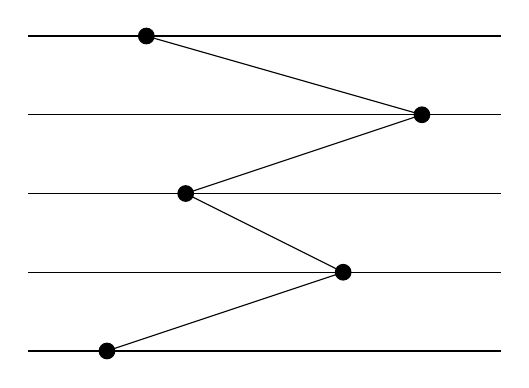
\begin{tikzpicture}[inner sep=0.7mm]
	\begin{scope}[thin]
	\draw (-3,2) -- (3,2);
	\draw (-3,1) -- (3,1);
	\draw (-3,0) -- (3,0);
	\draw (-3,-1) -- (3,-1);
	\draw (-3,-2) -- (3,-2);
	\end{scope}
	\draw (-2,-2)--(1,-1)--(-1,0)--(2,1)--(-1.5,2);
	\path node at (-2,-2) [circle,draw,fill=black] {}
	node at (1,-1) [circle,draw,fill=black] {}
	node at (-1,0) [circle,draw,fill=black] {}
	node at (2,1) [circle,draw,fill=black] {}
	node at (-1.5,2) [circle,draw,fill=black] {};
	\end{tikzpicture}
	\end{figure}
	\end{comment}
	
	\section{Renormalization in field theories}
	Field theory is well defined at what we call \emph{tree-level}\footnote{The name comes from the fact that there are very few looped trees.}, meaning if we have no loops in our Feynman diagrams. Since tree-level usually contributes the most to some reaction's likelihood (due to coupling coefficients below 1), there is a lot to be learned from such simple cases. However, there is still much insight to gained from loop diagrams, especially in those cases where a reaction is impossible without a loop. Once we start calculating loops, we almost always encounter divergences. Since we have divergences, we have to think up a scheme to \emph{renormalise} the theory.
	
	\subsection{Wilson's approach}
	A simple and very intuitive way to look on renormalisation was shown by Wilson, where he introduced the concept of \emph{renormalisation flow}.\\
	
	Wilson's approach uses $\phi^4$-theory \cite{PeskinSchroeder} and the functional method to show the nature of renormalisation. As is usual, we introduce a momentum cut-off such that our momentum-space integrals do not diverge. Therefore, our partition function becomes
	
	\begin{align}
		\begin{split}
		Z[\mathcal{J}] &= \int\mathcal{D}\phi e^{i\int\left[\mathcal{L} + \mathcal{J}\phi\right]} \\
		&= \left( \prod_k\int d\phi(k) \right)e^{i\int\left[\mathcal{L} + \mathcal{J}\phi\right]} \:,
		\end{split}
	\end{align}
	
	\noindent where
	
	\begin{equation}
		\phi(k) = 0 \quad\forall |k|>\Lambda \:,
	\end{equation}
	
	\noindent and $\Lambda$ is the momentum cut-off parameter. Performing a Wick rotation and setting $\mathcal{J} = 0$, we get
	
	\begin{equation}
		Z[\mathcal{J}=0] = \int\left[\mathcal{D}\phi\right]_\Lambda e^{i\int\left[ \frac{1}{2}\left(\partial_\mu\phi\right)^2 + \frac{1}{2}m^2\phi^2 + \frac{\lambda}{4!}\phi^4\right]} \:,
	\end{equation}
	
	\noindent where $\left[\mathcal{D}\phi\right]_\Lambda$ is the integral over $\phi(k)$ with respect to $\Lambda$.\\
	
	We now choose to further reduce the momentum-space with the parameter $\{\beta\in[0,1]\}$ and assume we may separate our field as
	
	\begin{equation}
		\phi \mapsto \hat{\phi}\phi \quad\text{such that}\quad \hat{\phi} =  \begin{cases}
		 \phi(k) \: &,\:k\in[\beta\Lambda,\Lambda) \\
		 0 \: &,\:\text{otherwise}
		\end{cases}\:.
	\end{equation}
	
	With this decomposition, the partition function becomes
	
	\begin{align}
		\begin{split}
			Z[\mathcal{J}=0] = &\int\mathcal{D}\phi \exp\left(i\int\mathcal{L}\right) \\
			&\times\int\mathcal{D}\hat{\phi} \exp\left(i\int\left[ \frac{1}{2}\left(\partial_\mu\hat{\phi}\right)^2 + \frac{1}{2}m^2\hat{\phi}^2 + \lambda\left\{ \frac{1}{6}\phi^3\hat{\phi} + \frac{1}{4}\phi^2\hat{\phi}^2 + \frac{1}{6}\phi\hat{\phi}^3 + \frac{1}{4!}\hat{\phi}^4 \right\}\right]\right) \:.
		\end{split}
	\end{align}
	
	Terms quadratic in $\phi\hat{\phi}$ are zero since Fourier components with different momentum are orthogonal. We would like to construct an effective Lagrangian that applies in the range given by $\beta$, i.e we want to prove
	
	\begin{equation}
		Z[\mathcal{J}=0] = \int\left[\mathcal{D}\phi\right]_{\beta\Lambda} e^{-\int d^dx\mathcal{L}_{\text{eff}}(\phi)} \:.
	\end{equation}
	
	This we do by treating all terms proportional to both $\lambda$ and the mass term (since we assume $m^2\ll\Lambda^2$) as perturbations. The leading order term is the kinetic term,
	
	\begin{equation}
		\int\mathcal{L}_0 = \frac{1}{2}\int\frac{d^dk}{(2\pi)^d}\hat{\phi}^*k^2\phi\:,
	\end{equation}
	
	\noindent which leads to the Green's function
	
	\begin{equation}
	\contraction[2pt]{}{\hat{\phi}}{(k)}{\phi}\hat{\phi}(k)\phi(p) = \frac{1}{k^2}(2\pi)^d\delta^{(d)}(k+p)\Theta(k) \:,
	\end{equation}
	
	\noindent where $\Theta(k)$ is the step function,
	
	\begin{equation}
		\Theta(k) = \begin{cases}
		1\:,&\:|k|\in[\beta\Lambda,\Lambda)\\
		0\:,&\:\text{otherwise}
		\end{cases} \:.
	\end{equation}
	
	Knowing this, we expand the exponential with the $\phi^2\hat{\phi}^2$-term,
	
	\begin{equation}
		-\int d^dx \frac{\lambda}{4}\phi^2\contraction[2pt]{}{\hat{\phi}}{}{\hat{\phi}}\hat{\phi}\hat{\phi} = -\frac{1}{2}\int \frac{d^dk}{(2\pi)^d}\mu\phi(k)\phi(-k) \:,
		\label{EFT | eq | phi^2hatphi^2-term}
	\end{equation}
	
	\noindent where
	
	\begin{equation}
		\mu = \frac{\lambda}{2}\int_{|k|\in[\beta\Lambda,\Lambda)}\frac{d^dk}{(2\pi)^d}\frac{1}{k^2}\frac{\lambda}{(4\pi)^{d/2}\Gamma\left(\frac{d}{2}\right)}\frac{1-\beta^{d-2}}{d-2}\Lambda^{d-2}\:,
	\end{equation}
	
	\noindent is a function of $\beta$ and $\Lambda$. We see now, however, that equation (\ref{EFT | eq | phi^2hatphi^2-term}) could also come from expanding
	
	\begin{equation}
		e^{-\int d^dx \left(\frac{1}{2}\mu\phi^2 + \ldots\right)}\:,
	\end{equation}
	
	\noindent which means we consider $\mu$ to be an effective\footnote{The word \emph{effective} is, by convention, used in the sense that effectively, we would see this as a mass. Whether or not it truly is physical mass is perhaps a bit philosophical.} mass.\\
	
	The Green's function $\contraction[2pt]{}{\hat{\phi}}{(k)}{\phi}\hat{\phi}(k)\phi(p)$ can be written as a Feynman propagator \cite{PeskinSchroeder}:
	
	\begin{figure}[h]
		\centering
		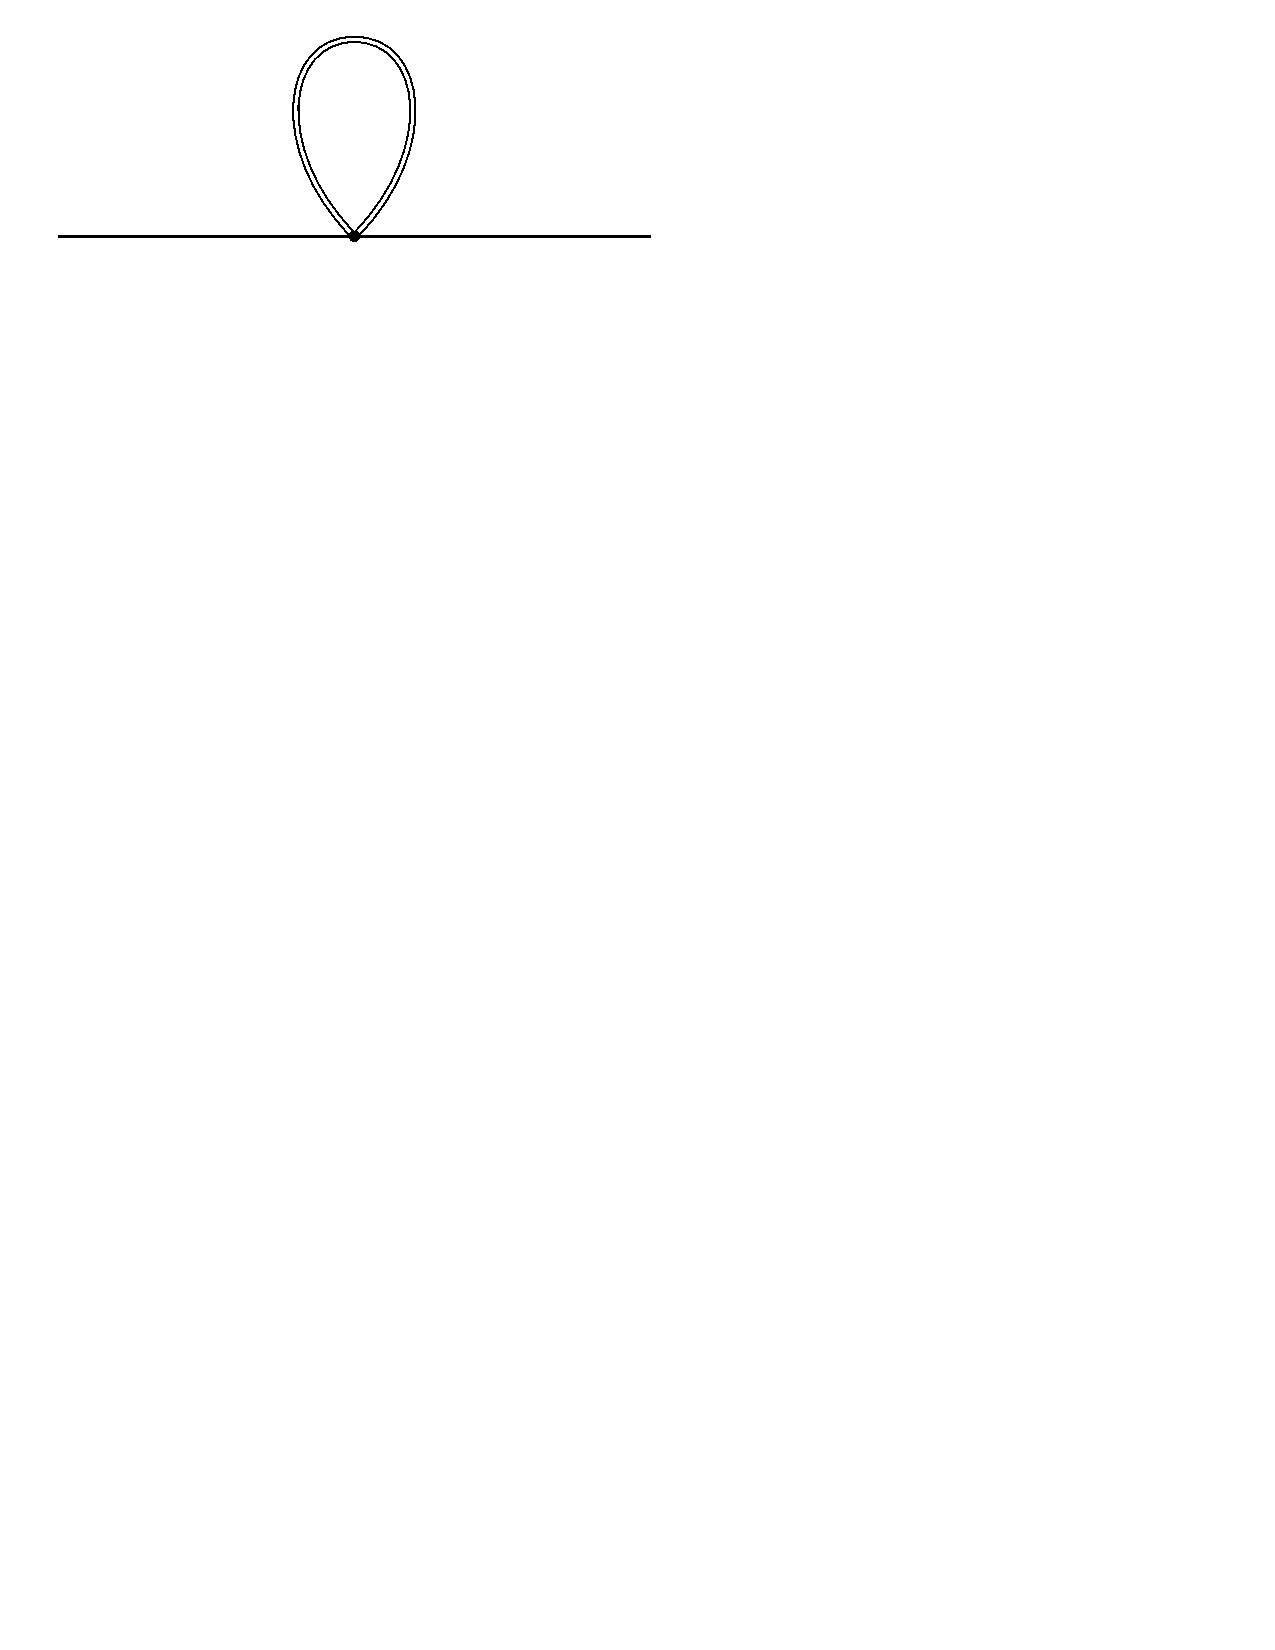
\includegraphics[trim={0.5cm 22cm 10cm 0cm},width=0.35\textwidth]{Figures/renorm1.pdf}
		\vspace{-0.5cm}
		\label{fey:2}
	\end{figure}
	
	Equation \ref{EFT | eq | phi^2hatphi^2-term} is a contribution to the scalar field propagator from high momentum fields ($\hat{\phi}$), which gives a contribution $\mu$ at order $\lambda$.
	If we consider diagrams of second order ($\mathcal{O}(\lambda^2)$), we have two possibilities \cite{PeskinSchroeder}:
	
	\begin{figure}[h]
		\centering
		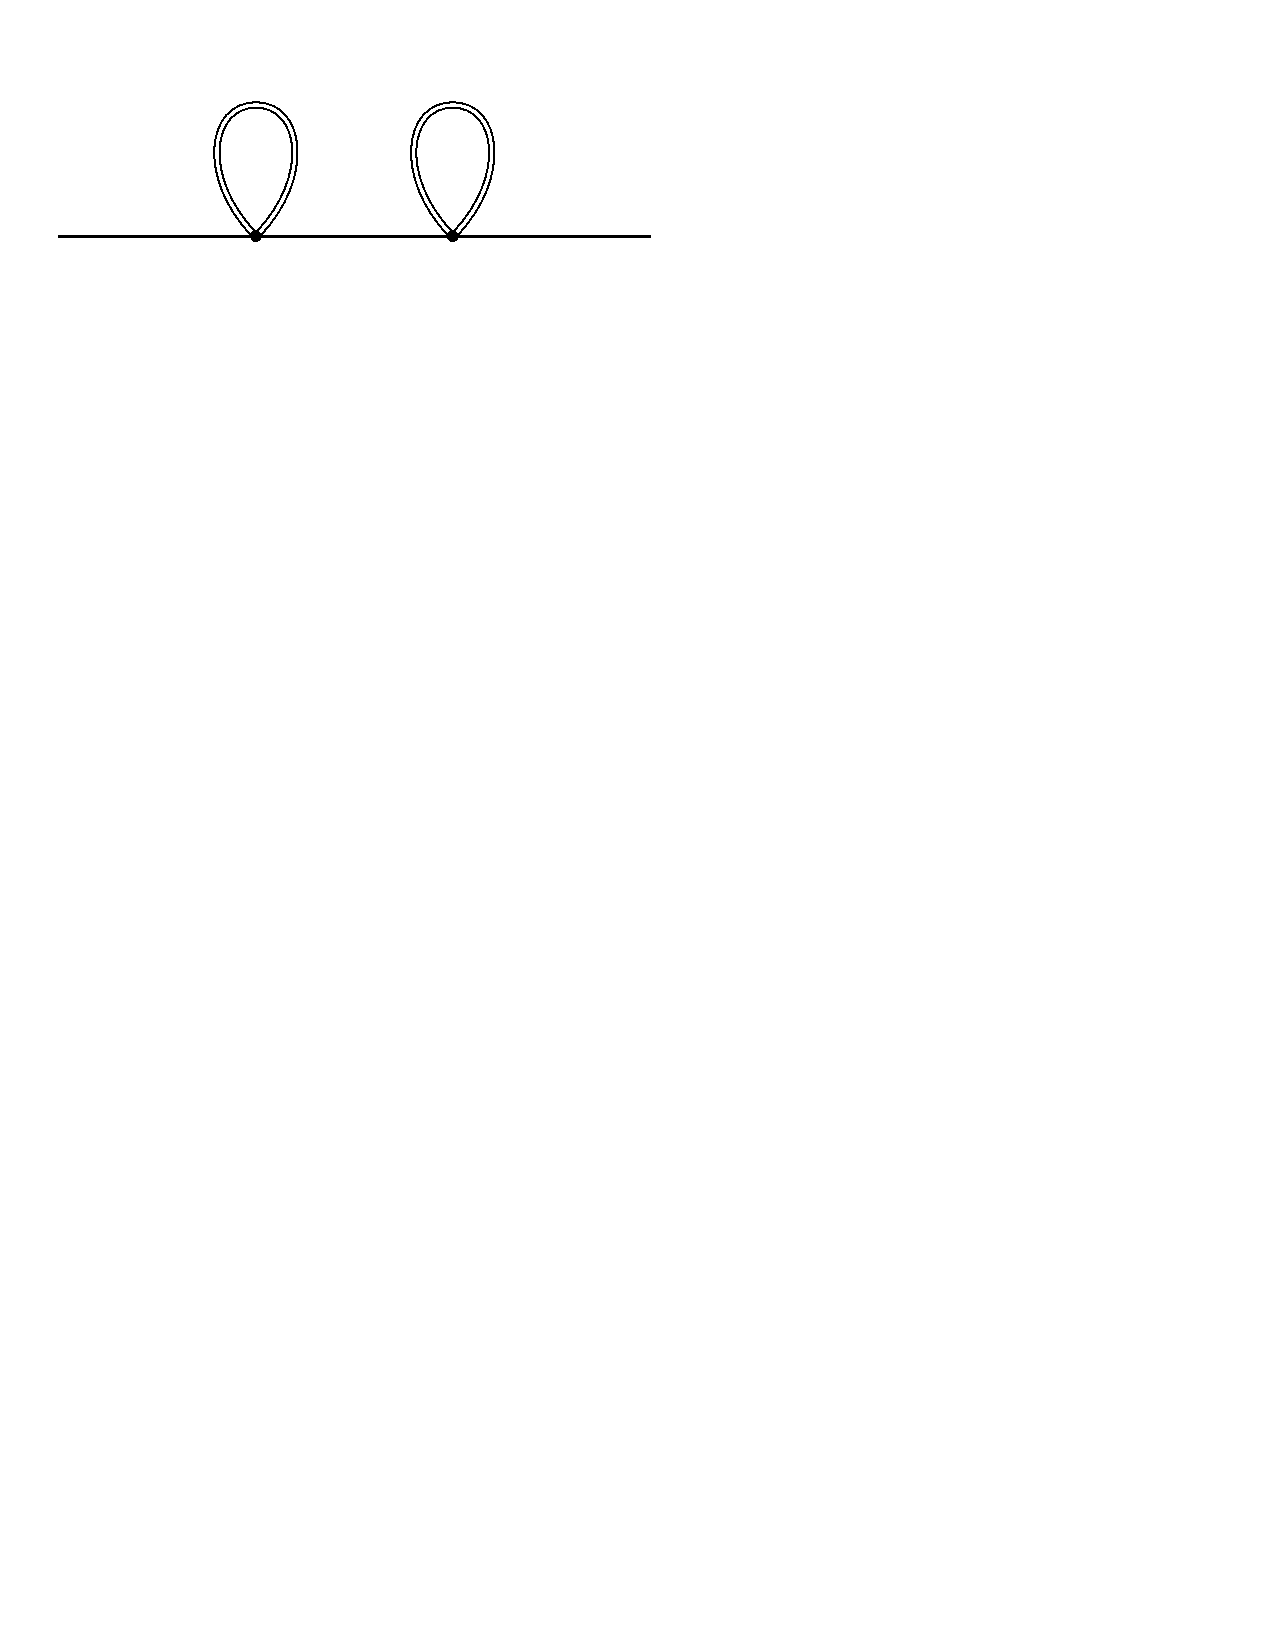
\includegraphics[trim={0.5cm 22cm 10cm 0cm},width=0.35\textwidth]{Figures/renorm3.pdf}
		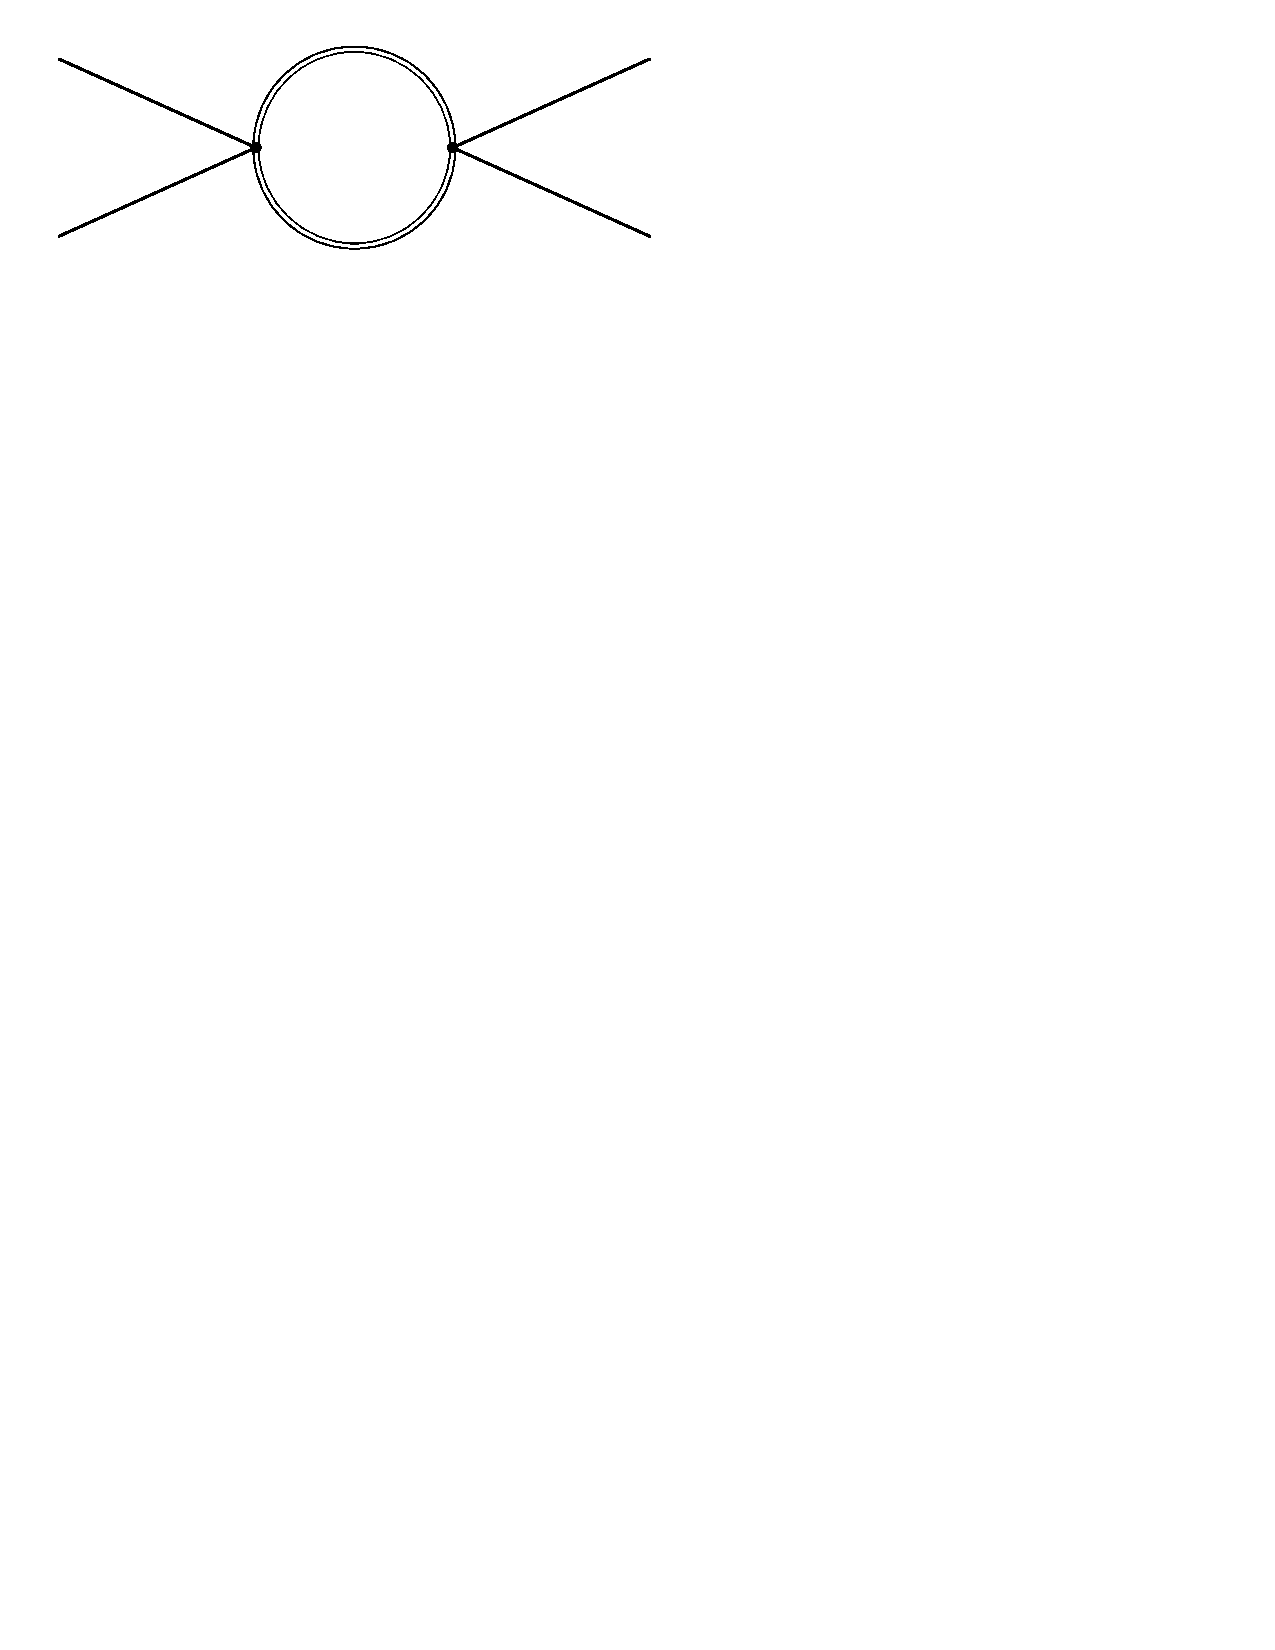
\includegraphics[trim={0.5cm 22cm 10cm 0cm},width=0.3\textwidth]{Figures/renorm2.pdf}
		\vspace{-0.25cm}
		\label{fey:3}
	\end{figure}
	
	The first diagram is merely a scalar-field self-interaction squared, and contributes to $\mu$ as well, except at higher order. The second diagram gives
	
	\begin{equation}
		-\frac{1}{4!}\int d^dx\zeta\phi^4 \:,
	\end{equation}
	
	\noindent where
	
	\begin{align}
		\begin{split}
		\zeta &= -4! \frac{2}{2!}\left(\frac{\lambda}{4}\right)^2\int_{|k|\in[\beta\Lambda,\Lambda)}\frac{d^dk}{(2\pi)^d}\frac{1}{k^2} \\
		&= \frac{-3\Lambda^2}{(2\pi)^{d/2}\Gamma\left(\frac{d}{2}\right)}\frac{1-\beta^{d-4}}{d-4}\Lambda^{d-4}\\
		\underset{d\rightarrow4}{\longrightarrow}&\: \frac{-3\lambda^2}{16\pi^2}\ln\left(\frac{1}{\beta}\right) \:.
		\end{split}
	\end{align}
	
	From this, we may interpret the ultraviolet divergence of the loop-diagram interaction as a contribution from all momentum scales ($\beta=(0\rightarrow1)$).\\
	
	We know disconnected diagrams do not contribute to the physical parameters, so we may define an effective Lagrangian as
	
	\begin{equation}
		\mathcal{L}_{\text{eff}} = \left(\partial_\mu\phi\right)^2 + \frac{1}{2}m^2\phi^2 + \frac{\lambda}{4!}\phi^4 + (\text{sum of all connected diagrams}) \quad,\:\text{where}\: |k|<\beta\Lambda
	\end{equation}
	
	Thus, we may indeed write an effective Lagrangian as proposed above.\\
	
	\subsubsection{Rescaling}
	Rather than working with functions of $\beta$, we wish to work in a scale-independent theory. If we choose to rescale length and momentum as
	
	\begin{align}
		\begin{split}
		k' &\equiv \frac{k}{\beta} \:,\\
		x' &\equiv \beta x \:.
		\end{split}
	\end{align}
	
	With the rescaling, we can quite easily show that if we also rescale the scalar field as
	
	\begin{equation}
		\phi' \equiv \left[\beta^{2-d}(1+\Delta Z)\right]^{1/2}\phi \:,
	\end{equation}
	
	\noindent and the physical constants as
	
	\begin{align}
		\begin{split}
			m'^2 &= \left(m^2 + \Delta m^2\right)(1+\Delta Z)^{-1}\beta^{-2} \\
			\lambda'^2 &= \left(\lambda + \Delta \lambda\right)(1+\Delta Z)^{-2}\beta^{d-4} \\
			&\vdots
		\end{split}
	\end{align}
	
	\noindent where the $\Delta$'s are small since they are diagram contributions, we get back the effective Lagrangian in the same form.\\
	
	We may now choose another $\beta$ (say $\beta'$), and again perform the rescaling. If we keep on doing such rescalings up until we reach $\Lambda$, we get a continuously varying effective Lagrangian. In other words, we get a Lagrangian that "flows" through some space of physical constants, or a "space of theories", if we are feeling poetic. The continuously generated transformations between Lagrangians is referred to as the \emph{renormalization group}.
	
	\subsection{Renormalized perturbation theory}
	The approach by Wilson is wonderfully instructive in understanding renormalization, but, sadly, impossible to apply in practical problems. Therefore, we turn to a much more gritty, but far more powerful, method called renormalized perturbation theory. When learning basic quantum field theory, we always work with perturbation theory when using Feynman diagrams. For example, $\phi^4$-theory uses a small constant $\lambda$, such that we may ignore higher order terms. Similarly, QED has the electronmagnetic coupling constant $\alpha_e \simeq \frac{1}{137}$, which allows us to ignore higher order terms and still find physically measurable results. QCD is not so forgiving, since the strong coupling constant fulfils $g_s \simeq 1$ at low energies, making it impossible to use perturbation theory. Other methods have to be used to do analysis on low energy, nuclear systems. \emph{Lattice QCD} (LQCD) is becoming a more and more common approach, but still suffers from high computational demands. Currently we are experiencing a period of great growth in the computer industry, which has allowed for more and more complicated LQCD calculations. However, LQCD encounters difficulties for real pion masses, and has so far had to use unphysical, lighter pions masses to perform calculations on nuclear systems. \emph{Chiral perturbation theory} (ChPT) does not suffer from such problems, but is not without fault either. ChPT introduces many new constants for each tier in the perturbation expansion. These constants must be known for ChPT to be of any use. So far, they have either been determined from experiment, or from LQCD calculations.\\
	
	To those still new to renormalization, it might comes as a bit of a shock to learn that the perturbation theory they have learned so far, may simply be considered as a certain limit of a renormalized perturbation theory. Furthermore, renormalized perturbation theory follows almost exactly the same rules as those for "normal" perturbation theory, except we know a bit more about the physical constants we use.\\
	
	There is one tool which we will use in the following chapter, called \emph{dimensional regularisation}. When a loop-integral diverges, we may treat the integral over spacetime as a continuous function of dimension, i.e. we replace $d^4x$ by $d^dx$. What we would then find (see \cite{PeskinSchroeder} for examples) is that the integral separates into a analytical solvable part and a part that diverges when we take the limit $d\rightarrow 4$. However, since we know that the scattering matrix is a physical quantity, mathematical divergences are not real. This serves as motivation to ignore divergent contributions. We will not go into the details of dimensional regularisation as it is not used extensively in our explanation of the next topic.
	
	\section{The Callan-Symanzik equation}
	Without a more formal approach, renormalized perturbation theory runs into problems when using zero mass fields. \\
	
	We decide to introduce new renormalization conditions, such that the two-point Green's function is zero at $p^2=-M^2$, and the four-point Green's function is equal to $-i\lambda$ at $s^2 = t^2 = u^2 = -M^2$, with $s,t,u$ being the Mandelstam variables.\\
	
	Consider the rescaled $n$-point Green's function:
	
	\begin{equation}
		G^{(n)}(\{x_i\}) = \langle\Omega|T[\psi(x_1)\ldots\psi(n_n)]|\Omega\rangle = Z^{n/2}\langle\Omega|T[\psi_0(x_1)\ldots\psi_0(n_n)]|\Omega\rangle
	\end{equation}
	
	If we do a small shift in the theory parameters,
	
	\begin{align}
		\begin{split}
			M \:&\mapsto\: M+\delta M \\
			\lambda \:&\mapsto\: \lambda+\delta \lambda \\
			\psi \:&\mapsto\: (1+\delta\eta)\psi
		\end{split}
	\end{align}
	
	\noindent then the change in the Green's function is
	
	\begin{equation}
		dG^{(n)} = \frac{\partial G^{(n)}}{\partial M}\delta M + \frac{\partial G^{(n)}}{\partial \lambda}\delta \lambda = n\delta\eta G^{(n)}
	\end{equation}
	
	Multiplying by $\frac{M}{\delta M}$ and defining $\beta \equiv \frac{M}{\delta M}\delta\lambda$ and $\gamma \equiv - \frac{M}{\delta M}\delta \eta$, this becomes:
	
	\begin{equation}
		\left[ M\frac{\partial}{\partial M} + \beta\frac{\partial}{\partial \lambda} + \eta\gamma \right]G^{(n)}(\{x_i\};M,\lambda) = 0
	\end{equation}
	
	\noindent which is the Callan-Symanzik equation.
	
	\newpage
	\chapter{Chiral Perturbation Theory}
	With a better grasp of the EFT formalism, we can now apply it to nuclear systems. Nuclear matter consists of, to no one's surprise, protons and neutrons. These particles are the constituents of our large-scale nuclear system, and QCD provides the detailed analysis of them and their interaction. As we have already given a brief historical account for Chiral perturbation theory (ChPT) we will not repeat ourselves. ChPT provides an effective field theory derived from QCD.
	
	\section{Quantum chromodynamics and $SU(3)$}
	Quantum chromodynamics (QCD for short) allows us to model the so-called strong nuclear force, named thus due to it's role in the behaviour of nuclei and nuclear interactions. The participants in the theory are \emph{quarks} and \emph{gluons}, elementary particles in the standard model of particle physics. Quarks and gluons are special as they carry a so-called \emph{colour} charge, of which there are three; red, blue, and green\footnote{Its best to mention now that "colour" is simply a word, without any relation to the concept of colour as perceived in everyday life (the way we perceive photon frequencies). The colour charge is only used to distinguish between the possible quantum states for these particles.} (conventionally). In short, quarks and gluons have another set of quantum numbers not available to the other elementary particles, and quantum chromodynamics model the interactions that take place in "colour space".\\
	
	%I need a note on classical and quantum Yang-Mills theories here.\\
	
	Quantum chromodynamics is fundamentally different from electroweak theory, in that it has asymptotic freedom. The strong interaction has it's name with good reason, but at high energies, like those achieved in particle accelerators, we see that protons tend to "fragment" at much weaker energies than we first expected. This is where, in 1973, it was postulated that quark structures are more weakly bound at higher energies, i.e. that quarks have asymptotic freedom. Furthermore, the quantum Yang-Mills theory for the strong interaction had to fulfil the following conditions \cite{JaffeWitten}:
	
	\begin{enumerate}
		\item \emph{Mass gap}: There must exist some lower energy limit $\Delta > 0$ such that all vacuum excitations have an energy $E\geq \Delta$.
		\item \emph{Quark confinement}: Quark fields transform non-trivially under $SU(3)$, but quark structures do not (baryons, mesons).
		\item \emph{Chiral symmetry breaking}: The vacuum (ground state) is potentially invariant only under a certain symmetry subgroup of $SU(3)$.
	\end{enumerate}
	
	The conditions explain, respectively, why nuclear forces are strong and short-ranged, why we never see isolated quarks, and why soft pions have current algebra. Current algebra will be explained later.
	
	\subsection{The Lagrangian density of QCD}
	The degrees of freedom offered by the colour property means that the irreducible representation of the special unitary group $SU(3)$ fits nicely, as it also has three degrees of freedom. Deriving the QCD Lagrangian by the gauge principle is done as follows; starting with the free Lagrangian
	
	\begin{equation}
	\mathcal{L}_{\text{free}} = \sum_f \bar{q}_f\left(i\slashed \partial - m_f\right)q_f \:,
	\end{equation}
	
	\noindent where $q_f$ is a Dirac spinor for flavour\footnote{We use the word \emph{flavour} to tell which quark type we are talking about. There are six quark flavours ("up" ($u$), "down" ($d$), "strange" ($s$), "charm" ($c$), "bottom" ($b$), "top" ($t$)), as well as six lepton flavours ("electron" ($e^-$), "electron-neutrino" ($\nu_e$), "muon" ($\mu^-$), "muon-neutrino" ($\nu_\mu$), "tau lepton" ($\tau$), "tau neutrino" ($\nu_\tau$)).} type $f$, a $SU(3)$ field transformation is performed,
	
	\begin{equation}
	q_f^\alpha \:\rightarrow\: U^\alpha_\beta q_f^\beta \:,
	\end{equation} 
	
	\noindent where $U = e^{-ig_s\frac{\lambda^a}{2}\theta_a}$ and $\lambda^a$ are the Gellmann matrices in the fundamental representation. As is standard, now locality is demanded: $\theta_a \:\rightarrow\: \theta_a(x)$. Of course, the problem now is that the Lagrangian is not invariant under such a transform, so a covariant derivative must be found.\\
	
	In non-Abelian gauge theory, for local invariance under some symmetry (Lie\footnote{See appendix \ref{Appendic A | Lie groups} for a quick introduction to Lie groups.}) group ($\psi \:\rightarrow\: V(x)\psi$), the unitary matrix $V(x)$ can be expanded infinitesimally about $x$:
	
	\begin{equation}
	V(x) = 1 + i\alpha^i(x)t^a + \mathcal{O}(\alpha^2)\:,
	\end{equation}
	
	\noindent where $t^a$ are the generators of the group and $\alpha^i$ some rotation. We can express the covariant derivative along a vector $n^\mu$ as
	
	\begin{equation}
	n^\mu D_\mu\psi = \lim_{\epsilon\:\rightarrow\:0} \frac{1}{\epsilon}\left[\psi(x+\epsilon x) - U(x+\epsilon x,x)\psi(x)\right]\:,
	\label{Def_of_D}
	\end{equation}
	
	\noindent where
	
	\begin{equation}
	U(y,x) \:\rightarrow\: V(y)U(y,x)V^\dagger(x)\:.
	\end{equation}
	
	So by infinitesimal expansion, in the case of $SU(3)$ ($V(x) = e^{-ig_s\frac{\lambda^a}{2}\theta_a(x)}$), we get
	
	\begin{equation}
	U(x+\epsilon, x) = 1 + ig_s\epsilon n^\mu G_\mu^a \lambda_a + \mathcal{O}(\epsilon^2)\:.
	\end{equation}
	
	Here $G_\mu^a$ are the gauge fields of $SU(3)$, later to be identified with the gluon fields. The absence of $\theta$ from $V$ is due to the details of the expansion. When inserting the above in equation (\ref{Def_of_D}) and taking the limit, it follows that
	
	\begin{equation}
	D^\mu q_f = \left[ \partial^\mu - ig_s\frac{\lambda^a}{2}G_a^\mu(x) \right]q_f \:.
	\end{equation}
	
	Thus the first order interactive term between the quarks and gluons is found, but the gauge-invariant kinetic gluon term remains hidden. Again, from non-abelian gauge theory it is known that the field strength must be found. The covariant derivative transforms as
	
	\begin{equation}
	D^\mu \:\rightarrow\: UD^\mu U^\dagger\:.
	\end{equation}
	
	This is known because $D^\mu q_f$ is invariant, and since $U$ is unitary, we have
	
	\begin{equation}
		D^\mu q_f \:\rightarrow\: UD^\mu q_fU^\dagger = UD^\mu U^\dagger U q_fU^\dagger\:
	\end{equation}
	
	So, the above transform means the gluon field transforms as
	
	\begin{equation}
	G^\mu \:\rightarrow\: UG^\mu U^\dagger - \frac{i}{g_s}(\partial^\mu U)U^\dagger\:.
	\end{equation}
	
	This is obviously not then an invariant quantity. Instead, we can introduce a tensor,
	
	\begin{align}
		\begin{split}
		G^{\mu\nu}(x) &\equiv \frac{i}{g_s}[D^\mu,D^\nu]\\
		&= \partial^\mu G^\nu - \partial^\nu G^\mu - ig_s[G^\mu,G^\nu]\\
		&\equiv \frac{\lambda^a}{2}G_a^{\mu\nu}(x)\:,
		\end{split}
	\end{align}
	
	\noindent where
	
	\begin{equation}
	G_a^{\mu\nu} = \partial^\mu G_a^\nu - \partial^\mu G_a^\nu + g_sf^{abc}G_b^\nu G_c^\nu\:,
	\end{equation}
	
	\noindent and $f^{abc}$ is the group structure constant. Now we have an invariant term,
	
	\begin{equation}
	G^{\mu\nu} \:\rightarrow\: UG^{\mu\nu}U^\dagger\:.
	\end{equation}
	
	In order to get kinetic terms, and to remove the free indices, the final Lagrangian is
	
	\begin{equation}
	\mathcal{L}_{\text{QCD}} = -\frac{1}{4}G_a^{\mu\nu}G_{\mu\nu}^a + \sum_f \bar{q}_f(i\gamma^\mu D_\mu - m_f)q_f\:.
	\end{equation}
	
	This appears to be identical to the QED Lagrangian. However, there are important differences. The biggest difference between the QED and QCD Lagrangian lies of course in the "force carriers", where there exists one photon, but eight gluons. This means that whereas there or no photon-photon couplings, there are gluon-gluon couplings. Additionally, the electric charge in the QED Lagrangian is unique for each fermion. In QCD, the colour charge is the same for all fermions. This is tied to QED employing $U(1)$, i.e. the transformation of each fermion was linear such that the "coefficients" are free to be chosen. In $SU(3)$, however, the transformations are non-linear ($\lambda_a$ and $\lambda_b$ determine $\lambda_c$). As such, $g_s$ is the same for all fermions - the strong coupling constant.
	
	\section{Symmetries in quantum mechanics}
	While we have already discussed the symmetries of wave functions and the spin-statistics theorem, we have not really discussed symmetries in general. It perhaps seems superfluous to start with the basics, however we will need them to move onto the chiral symmetry, and the consequences of breaking it with the reintroduction of massive quark fields.
	
	\subsection{Noether's theorem}
	Before delving right into symmetries and their connection with conserved currents and charges, a brief reminder of \emph{Noether's theorem} needs to be given. Due to the importance of symmetry in physics, most undergraduate physicists have some knowledge of the theorem. However, it's rarer to understand it in the context of quantum mechanics and field theories, and even less so in quantum field theories.\\
	
	In classical mechanics, Noether's theorem uses the invariance of the Lagrangian under some symmetry to show that some quantities remain unaltered. Examples of this are angular momentum, which remains unaltered by a angular transformation of the system coordinates, and the stress-energy tensor, which is found to be conserved when performing a Lorentz transform.\\
	
	Consider a classical action $S_{C}$ defined as the path-integral for some given Lagrangian $L_{C}$:
	
	\begin{equation}
		S_{C} = \int d^3x \:L_{C}(\Phi,\Pi,\bm{x})\:,
	\end{equation}
	
	\noindent where $\Phi := \left\{\phi_1,\phi_2,\ldots,\phi_n\right\}$ and  $\Pi := \left\{\partial_\mu\phi_1,\partial_\mu\phi_2,\ldots,\partial_\mu\phi_n\right\}$ are canonical coordinates, and $\bm{x}$ are coordinates in $\mathbb{R}^3$ (3-dimensional Euclidean space). If $S_C$ does not change when we change, or transform, the system coordinates, we say we have a symmetry under the group from which that kind of transform originates.\\
	An example is  rotating a $\mathbb{R}^3$ coordinate system, which means acting on the basis vectors with the rotational matrices. These matrices are actually \emph{one} representation of the Lie group $SO(3)$. Therefore, we say a system is $SO(3)$ invariant if 3-dimensional rotations change nothing\footnote{If the reader finds this case a little too trivial, consider a system where inversion of one coordinate, say $x\rightarrow -x$, changes nothing. We then say a system has a $\mathbb{R}\setminus\mathbb{Z}_2$ symmetry; a real line $\mathbb{R}$, where each positive number is equivalent to the respective negative number ($\mathbb{Z}_2$ symmetry), except zero, which has no "inverse".}.\\
	
	Now, given some Lagrangian $L_C$, we may use the Euler-Lagrange equations,
	
	\begin{equation}
		\left(\frac{\partial}{\partial \phi_i} - \frac{d}{dt}\frac{\partial}{\partial \left(\partial_\mu \phi_i\right)}\right)L_C = 0\:,
	\end{equation}
	
	\noindent to prove Noether's theorem.
	
	\subsubsection{Noether's theorem in classical field theory: Conserved currents}
	The classical field version of Noether's theorem follows quite naturally. Assuming the Lagrangian depends on fields $\Phi_i$ and conjugate fields $\Pi_i=\partial_\mu\Phi_i$, the Euler-Lagrange equations of motion look like
	
	\begin{equation}
		\frac{\partial\mathcal{L}}{\partial\Phi_i} - \partial_\mu\left(\frac{\partial\mathcal{L}}{\partial\Pi_i}\right) = 0\:.
		\label{ChPtTh | eq | euler-lagrange for fields}
	\end{equation}
	
	We know $\mathcal{L}$ is invariant under some global transformation. To promote it to a local one, we study which effect a local transformation has. So we start by writing the transformations of the fields as
	
	\begin{align}
		\begin{split}
			\Phi_i(x) \mapsto \:& \Phi_i(x) + \delta\Phi_i(x) \\
			&= \Phi_i(x) - i\epsilon_a(x)F_{ai}[\Phi(x)]\:,
		\end{split}
	\end{align}
	
	\noindent where $\epsilon_a(x)$ is the $a$'th transformation of $\Phi_i(x)$, and $F_ai$ is the transformation generator. With this knowledge, we find the change in the Lagrangian
	
	\begin{align}
		\begin{split}
			\delta\mathcal{L} &= \mathcal{L}' - \mathcal{L}\\
			&= \frac{\partial\mathcal{L}}{\partial\Phi_i}\delta\Phi_i + \frac{\partial\mathcal{L}}{\partial(\partial_\mu\Phi_i)}\partial_\mu(\delta\Phi_i) + \mathcal{O}(\epsilon^2) \\
			&= \epsilon_a\left[ -i\frac{\partial\mathcal{L}}{\partial\Phi_i}F_{ai} - i\frac{\partial\mathcal{L}}{\partial(\partial_\mu\Phi_i)}\partial_\mu F_{ai} \right] + \partial_\mu\epsilon_a\left[ -i\frac{\partial\mathcal{L}}{\partial(\partial_\mu\Phi_i)}F_{ai} \right] \\
			&= \epsilon_a\partial_\mu( J_a^\mu) + \partial_\mu( \epsilon_aJ_a^\mu)\:,
		\end{split}
	\end{align}
	
	\noindent where we defined
	
	\begin{align}
		J_a^\mu &= -i\frac{\partial\mathcal{L}}{\partial(\partial_\mu\Phi_i)}F_{ai} \\
		\partial_\mu(J_a^\mu) &= -i\partial_\mu\left(\frac{\partial\mathcal{L}}{\partial(\partial_\mu\Phi_i)}\right)F_{ai} - i\frac{\partial\mathcal{L}}{\partial(\partial_\mu\Phi_i)}\partial_\mu F_{ai}\:.
	\end{align}
	
	From the equation of motion (\ref{ChPtTh | eq | euler-lagrange for fields}), we see $\partial_\mu(J_a^\mu)=0$. Therefore, our Noether currents are now
	
	\begin{align}
		J_a^\mu &= \frac{\partial (\delta\mathcal{L})}{\partial(\partial_\mu\epsilon_a)} \\
		\partial_\mu J_a^\mu &= \frac{\partial (\delta\mathcal{L})}{\partial\epsilon_a} = 0
	\end{align}
	
	\subsubsection{Noether's theorem in quantised field theory: Ward-Takahashi identities}
	The quantised field theory version of Noether's theorem is quite similar to the classical version, although there are some small differences. Following the example of \cite{PeskinSchroeder}, we consider a set of local fields $\{\varphi_a(x)\}$ that generally transform locally as
	
	\begin{equation}
		\varphi_a(x) \mapsto \varphi_a(x) + \epsilon(x)\Delta\varphi_a(x)\:.
	\end{equation}
	
	Assuming that some Lagrangian $\mathcal{L}(\{\varphi_a\})$ is invariant under this symmetry, then from the functional integral, we expect the Lagrangian to be invariant up to\footnote{With an implied summation of $a$.}
	
	\begin{equation}
		\mathcal{L}(\{\varphi_a\}) \mapsto \mathcal{L}(\{\varphi_a\}) + (\partial_ \mu\epsilon(x))\Delta\varphi_a \frac{\partial\mathcal{L}}{\partial(\partial_ \mu\varphi_a)} + \epsilon(x)\partial_\mu\mathcal{J}^\mu\:,
	\end{equation}
	
	\noindent with $\mathcal{J}^\mu$ being our generating functional. The change in the action $S$ with respect to $\epsilon(x)$ is therefore
	
	\begin{equation}
		\frac{\delta}{\delta(\epsilon(x))}\int d^4x \mathcal{L} = -\partial_\mu j^\mu(x)\:,
	\end{equation}
	
	\noindent where
	
	\begin{equation}
		j^\mu(x) = \Delta\varphi_a \frac{\partial\mathcal{L}}{\partial(\partial_ \mu\varphi_a)} + \partial_\mu\mathcal{J}^\mu
	\end{equation}
	
	\noindent is the Noether current. By continuing to calculate the correlation function, as we usually do in the path integral formulation, we find \cite{PeskinSchroeder} the \emph{Schwinger-Dyson} equations,
	
	\begin{align}
		\begin{split}
		\langle j_\mu(x)\varphi_a(x_1)\varphi_b(x_2)\ldots\varphi_m(x_n)\rangle = (-i)\big\langle &(\varphi_a(x_1)\delta(x-x_1))\varphi_b(x_2)\ldots\varphi_m(x_n) \\
		&+\varphi_a(x_1)(\varphi_b(x_2)\delta(x-x_2))\ldots\varphi_m(x_n) \\
		&\:\vdots\\
		&+\varphi_a(x_1)\varphi_b(x_2)\ldots(\varphi_m(x_n)\delta(x-x_n))\big\rangle\:.
		\end{split}
	\end{align}
	
	These equations are usually called \emph{Ward-Takahashi identities}, which are equations that the correlation function must satisfy if the Lagrangian is invariant under some symmetry. It is common to express these equations in terms of the invariant scattering element $\mathcal{M}$, and rather talk in terms of momentum rather than position, as they were first expressed by J.C. Ward and Y. Takahashi.
	
	\section{The Chiral Limit}
	Earlier, we discussed the part of the standard model that concerns the strong nuclear force. However, chiral perturbation theory is built upon the \emph{chiral limit}, i.e. when we let the quark masses approach zero. At this limit, there is no mixing between the helicity states of quarks, and as such, we may let the left- and right-handed parts of the quark fields transform separately. In other words, our $SU(3)$ symmetry is now  written $SU(3)_L\times U(1) \times SU(3)_R\times U(1)$, allowing us to move onto vector and axial-vector representations.
	
	\subsection{Group decomposition}
	In the chiral limit, flavour becomes a $SU(3)\times U(1)$-symmetry. That is, rotations between quark flavours have no effect on our Lagrangian, and the quark fields are invariant up to a complex phase, represented by $U(1)$-transformations. This might seem somewhat superfluous to mention at all, since we may usually pull the complex phases out of any amplitude calculations, thus having no effect. However, it turns out to be not quite that simple. When introducing quark masses, the symmetries are broken, and we would expect massless Goldstone bosons to appear for every broken symmetry. We shall find that, while particles that correspond to pseudoscalar mesons appear, there are no known particles that correspond to the $U(1)$-symmetry breaking. The reason is provided by the appearance of an \emph{anomaly}, which we shall discuss in section \ref{subSec | Chiral anomaly}. If we decide to treat the left- and right-handed parts of each quark field separately, then we get a $SU(3)_L\times SU(3)_R$ symmetry group, which shall serve as our starting point.
	
	\subsection{Symmetry currents in the chiral limit}
	Since quarks are $SU(2)$ spinors, we know from basic QFT that they may be decomposed into left- and right-handed representations
	
	\begin{equation}
	q(x) = (P_R+P_L)q(x) = q_R(x) + q_L(x)\:,
	\end{equation}
	
	\noindent where $P_{L/R}$ are the left \& right projection operators, and have the identities
	
	\begin{align}
		P_{L/R}^2 &= P_{L/R}\:, \\
		P_{R} + P_{L} &= \mathds{1}\:, \\ 
		\left(P_{L/R}\right)\left(P_{R/L}\right) &= 0 \:.
	\end{align}
	
	To the reader unacquainted with left- and right-handedness, a quantum field that exists in several (not physical) dimensions (say in the Lie group $SU(N)$) can be broken down into its dimensional constituents (like any vector).\\
	
	The interaction terms we have between quark fields go as $\bar{q}\Gamma q$, where $\Gamma$ symbolizes any of the Dirac field bilinears, such that in general
	
	\begin{equation}
	\bar{q}\Gamma q = \begin{cases}
	&\bar{q}_R\Gamma q_R + \bar{q}_L\Gamma q_L \quad\text{for}\quad \Gamma=\{\gamma^\mu, \gamma^\mu\gamma_5\}\\
	&\bar{q}_R\Gamma q_L + \bar{q}_L\Gamma q_R \quad\text{for}\quad \Gamma=\{\mathds{1}, \gamma_5, \sigma^{\mu\nu}\}
	\end{cases} \:.
	\end{equation}
	
	This applies outside the chiral limit as well. We can now express $\mathcal{L}^{(0)}$ (QCD Lagrangian) in terms of left- and right-handed projections,
	
	\begin{equation}
	\mathcal{L}^{(0)} = -\frac{1}{4}G_a^{\mu\nu}G_{\mu\nu}^a + \sum_{f} \left( \bar{q}_{f,R}i\slashed Dq_{f,R} + \bar{q}_{f,L}i\slashed Dq_{f,L} \right)\:.
	\end{equation}
	
	Since the Dirac equation is flavour independent, the Lagrangian is invariant under the product group $G=U_L(3)\times U_R(3)$. This is a classical global symmetry. Since the product group is diffeomorphic to $G'=SU_L(3)\times SU_R(3)\times U_L(1)\times U_R(1)$, we may choose to represent the transformations under $G$ as those of $G'$, such that
	
	\begin{align}
		q_R &\mapsto \exp\left( -i\sum_{a=1}^8 \Theta_{Ra}\frac{\lambda_a}{2} \right)e^{-i\Theta_R}q_R\:, \\
		q_L &\mapsto \exp\left( -i\sum_{a=1}^8 \Theta_{La}\frac{\lambda_a}{2} \right)e^{-i\Theta_L}q_L\:.
	\end{align}
	
	If we werer to calculate Noether currents now (see \cite{SchererSchingler12}), we would find six conserved currents,
	
	\begin{align}
		L_i^\mu &= \bar{q}_L\gamma^\mu\frac{\tau_i}{2}q_L\:, \\
		R_i^\mu &= \bar{q}_R\gamma^\mu\frac{\tau_i}{2}q_R\:.
	\end{align}
	
	We may also construct linear combinations,
	
	\begin{align}
		V_i^\mu &= L_i^\mu + R_i^\mu\:, \\
		A_i^\mu &= L_i^\mu - R_i^\mu\:,
	\end{align}
	
	\noindent which we recognise as the \emph{vector} and \emph{axial-vector} currents.
	
	We finally end up with the $SU(2)_L\times SU(2)_R$ algebra, which we henceforth refer to as the \emph{chiral algebra}:
	
	\begin{equation}
	\left[Q_I^i, Q_I^j\right] = if^{ijk}Q_I^k \quad \text{for}\quad I=R,L
	\end{equation}
	
	\begin{equation}
	\left[Q_L^i, Q_R^j\right] = 0
	\end{equation}
	
	\noindent or equivalently, but written in axial- and vector-representations, we have
	
	\begin{align}
		\left[Q_V^i, Q_V^j\right] &= if^{ijk}Q_V^k \\
		\left[Q_A^i, Q_A^j\right] &= if^{ijk}Q_V^k \\
		\left[Q_V^i, Q_A^j\right] &= if^{ijk}Q_A^k 
	\end{align}
	
	The chiral algebra is quite important when developing meson theory, because we will see that each conserved current may be tied to a real meson particle. In the case of pseudoscalar fields, we will find the all-too familiar \emph{pion} ($\pi$).
	
	\subsection{Chiral anomaly}\label{subSec | Chiral anomaly}
	Sometimes, when quantizing a classical theory, a term appears that violates a symmetry of the classical theory. We name such a term an \emph{anomaly}. In the case of axial and vector currents, it turns out that Ward identities associated with them cannot be simultaneously be fulfilled, due to triangle-graphs. The Green's functions for the axial-vector and vector currents are given by
	
	\begin{align}
		\langle0&|T j_\mu(x)j_\nu(y)j_ \lambda^5(z)|0\rangle\:, \\
		\langle0&|T j_\mu(x)j_\nu(y)P(z)|0\rangle \:.
	\end{align}
	
	The Ward identities are derived as discussed earlier, by differentiating the Green's functions. We start with the axial current:
	
	\begin{align}
		\begin{split}
		q^\lambda T_{\mu\nu\lambda} &= \int d^4x\:d^4y\:d^4z\:e^{i(k_1x + k_2y - qz)} \partial_z^\lambda\langle0|T j_\mu(x)j_\nu(y)j_ \lambda^5(z)|0\rangle\\
		&= \int d^4x\:d^4y\:d^4z\:e^{i(k_1x + k_2y - qz)} \langle0|T j_\mu(x)j_\nu(y)\partial_z^\lambda j_ \lambda^5(z)|0\rangle \\
		&= 2mT_{\mu\nu}\:,
		\end{split}
	\end{align}
	
	\noindent where we have ignored all possible Schwinger terms and made use of $\partial^\mu j_\mu^5 = 2mP$ with $P=\bar{\psi}\gamma^5\psi$. Similarly, the vector WI is found by using $\partial_ \mu j^\mu = 0$, thus giving
	
	\begin{equation}
		k^\mu T_{\mu\nu\lambda} = k^\nu T_{\mu\nu\lambda} = 0 \:.
	\end{equation}
	
	However, this is not true if we do the same calculations by use of Feynman diagrams, and we shall see that it is due to the non-abelian properties of GROUP? Note that in the derivation of the axial WI, we made use of integration by parts, and of the Green function going to zero at infinity (the limit of our integrals). We failed to mention, however, that the Green's functions are singular, and as such they require renormalization. The renormalization scheme gives rise to non-zero terms at the integral limits. We shall see this soon.\\
	 
	The anomaly we find is that, if the vector WI is true, then the axial WI is violated by an additional term,
	
	\begin{align}
		q^\lambda T_{\mu\nu\lambda} &= 2mT_{\mu\nu} + A_{\mu\nu} \:, \\
		A_{\mu\nu} &= -\frac{1}{2\pi^2}\epsilon_{\mu\nu\rho\sigma}k_1^\sigma k_2^\rho \:.
	\end{align}
	
	ABJ-anomaly (Adler-Bell-Jackiw), as found through $\pi\:\rightarrow\:2\gamma$ decay
	
	\begin{equation}
	A = \frac{e^2}{16\pi^2}\epsilon^{\mu\nu\rho\sigma}F_{\mu\nu}F_{\rho\sigma} \:.
	\end{equation}
	
	Lastly, we would like to mention that there is far more insight to be found by considering the chiral anomaly in terms of the path integral method. Unfortunately, it requires quite a bit more groundwork, and is unnecessary for the use of ChPT as presented herein. For any physicist with a passion for connections between seemingly separate topics in physics, a deeper understanding of anomalies in QFTs, especially in the path-integral approach, ought certainly to be high on the "to do" list.
	
	\subsection{Mass terms}
	Despite the beauty of the chiral limit, it is not a real symmetry. Quarks are massive particles, and as such, we run into problems. The mass matrix, $M$, is
	
	\begin{equation}
	M = \begin{pmatrix}
	m_u & 0 & 0\\
	0 & m_d & 0\\
	0 & 0 & m_s
	\end{pmatrix}
	\end{equation}
	
	In QCD, this matrix is actually bigger, due to the remaining quarks; charm, bottom, and top. However, chiral perturbation theory is a low-energy effective theory, usually good for energies of less than 1 GeV\footnote{We will see later that this is due to what is called the \emph{chiral symmetry breaking scale}.}. The strange quark is the most massive particle that passes below this energy, with a mass of $m_s=95\pm5\:\text{MeV}$, and if we compare to the charm quark's mass, $m_s\simeq1.29\:\text{GeV}$, we see it is too high for ChPT. Our theory does not do well in describing interactions with charm, bottom, or top mesons. Therefore, ChPT usually only concerns itself with the strange nonet mesons, which we shall explain in more detail later on.
	
	\section{Spontaneous symmetry breaking}
	Spontaneous symmetry breaking is well known from its role in the Higgs mechanism, but such is far from its sole application. \emph{"Spontaneous symmetry breaking occurs when the ground state of a system does not possess the full symmetry of the theory"}\footnote{Citation source: https://arxiv.org/pdf/0912.4139v5.pdf, page 2}.
	
	
	\subsection{Goldstone's theorem and massless Goldstone bosons}
	Perhaps the most famous example of SSB and Goldstone bosons, is their application in the Higgs mechanism\footnote{Technically we should call it the ABEGHHK'tH mechanism, due to the role of many physicists in the theory's development. We will stick to the "Higgs mechanism" because it rolls better off the tongue.}. The Higgs mechanism was, at first, a theoretical model that showed that SSB will give mass to gauge bosons. Later, it was showed by Glashow, Weinberg, and Shalam that the Higgs mechanism could explain the masses of the weak gauge bosons, $W^\pm$ and $Z^0$, if they combined a $U(1)$-symmetry\footnote{Which is the QED symmetry group, meaning the symmetry group $SU(2)\times U(1)$ has 4 gauge bosons.} with the weak symmetry group ($SU(2)$). The theory became know as the \emph{electroweak model}. At the time, the theory would have enormous success, \emph{if} there had existed a another neutral, massive gauge boson, needed to explain the change in the vacuum expectation value. The field related to the change in the vacuum expectation value was named the Higgs boson. This is why, in 2013, the confirmation of the Higgs boson's existence was such an important event, as it was the finishing touch to the standard model as we know it today. Of course, the Higgs boson is of little concern to us, but it is nice to see the importance of SSB. Furthermore, we shall soon see how SSB and Goldstone bosons also play an important role in the chiral model.
	
	\subsubsection{Goldstone's theorem in general}
	To prove Goldstone's theorem in general \cite{EWeinberg11}, we can first consider the vacuum expectation value for some conserved current $J$
	
	\begin{align}
		\begin{split}
		\langle\Omega|[J^\lambda(y),\phi_n(x)]|\Omega\rangle &= \sum_N \left\{\langle\Omega|J^\lambda(y)|N\rangle\langle N|\phi_n(x)|\Omega\rangle - \langle\Omega|\phi_n(x)|N\rangle\langle N|J^\lambda(y)|\Omega\rangle\right\}  \\ 
		&= \sum_N \left\{e^{ip_N\cdot(x-y)}\langle\Omega|J^\lambda(0)|N\rangle\langle N|\phi_n(0)|\Omega\rangle - e^{-ip_N\cdot(x-y)}\langle\Omega|\phi_n(0)|N\rangle\langle N|J^\lambda(0)|\Omega\rangle \right\} \\
		&= \sum_N\int\frac{d^4k}{(2\pi)^4}\Big\{ \delta^{(4)}(p_N-k)e^{ik\cdot(x-y)}\langle\Omega|J^\lambda(0)|N\rangle\langle N|\phi_n(0)|\Omega\rangle\\
		&\hspace{2.1cm}
		 - \delta^{(4)}(p_N-k)e^{-ik\cdot(x-y)}\langle\Omega|\phi_n(0)|N\rangle\langle N|J^\lambda(0)|\Omega\rangle \Big\}\\
		\end{split} \:,
		\label{ChPT | eq | "vacuum exp val"}
	\end{align}
	
	where we have the identities,
	
	\begin{align}
		\sum_N\delta^{(4)}(p_N-k)\langle\Omega|J^\lambda(0)|N\rangle\langle N|\phi_n(0)|\Omega\rangle &= ip^\lambda\theta(k^0)\rho_a(k^2) \label{ChPtTh | eq | "intermediate eq 1"} \:,\\
		\sum_N\delta^{(4)}(p_N-k)\langle\Omega|\phi_n(0)|N\rangle\langle N|J^\lambda(0)|\Omega\rangle &= ip^\lambda\theta(k^0)\tilde{\rho}_a(k^2) \:.
	\end{align}
	
	We know that if $x^0 = y^0$ and $\bm{x} \neq \bm(y)$, then causality means the commutator is zero. If we also let $\bm{k}\rightarrow -\bm{k}$, we find $\tilde{\rho}_a(k^2) = \rho_a(k^2)$. Therefore, the above becomes
	
	\begin{equation}
		\langle\Omega|[J^\lambda(y),\phi_n(x)]|\Omega\rangle
		= -\frac{\partial}{\partial y^\lambda}\int\frac{d^4k}{(2\pi)^4}\rho_a(k^2)\theta(k^0)\left(e^{ik\cdot(x-y)} - e^{-ik\cdot(x-y)}\right) \:.
	\end{equation} 
	
	We can recognise the free field Green's function by inserting a Dirac delta like
	
	\begin{equation}
	\langle\Omega|[J^\lambda(y),\phi_n(x)]|\Omega\rangle
	= -\frac{\partial}{\partial y^\lambda}\int d\mu^2\rho_a(\mu^2)\underbrace{\int\frac{d^4k}{(2\pi)^4}\theta(k^0)\delta(\mu^2-k^2)\left(e^{ik\cdot(x-y)} - e^{-ik\cdot(x-y)}\right)}_{\text{Free field Green's function}} \:.
	\end{equation}
	
	The free field Green's function is zero for spacelike separations (which we assumed to have $\tilde{\rho}_a(k^2) = \rho_a(k^2)$). Now we use the conserved current property $\partial_\mu J^\mu = 0$, meaning our integral becomes:
	
	\begin{equation}
			0 = -\Box_y \int d\mu^2\rho_a(\mu^2)G(x-y) \:,
	\end{equation}
	
	\noindent where $G(x-y)$ is the free field Green's function. For timelike separations, we have $G(x-y)\neq 0$, so the remaining integrand must be zero:
	
	\begin{equation}
		\mu^2\rho_a(\mu^2) = 0 \Rightarrow \rho_a(\mu^2) = c_a\delta(\mu^2) \:,
	\end{equation}
	
	\noindent where $c_a$ is some constant. Considering the zero'th component of the vacuum expectation value, we insert our new knowledge of $\rho_a(\mu^2)$ (we also take the derivative)
	
	\begin{align}
		\begin{split}
		\langle\Omega|[J^0(y),\phi_n(x)]|\Omega\rangle &= 2i\int d\mu^2\rho_a(\mu^2)\int\frac{d^4k}{(2\pi)^4}\theta(k^0)\delta(\mu^2-k^2)k^0e^{i\bm{k}\cdot(\bm{x}-\bm{y})} \\
		&= 2i\int d\mu^2\rho_a(\mu^2)\underbrace{\int\frac{d^3k}{(2\pi)^3}e^{i\bm{k}\cdot(\bm{x}-\bm{y})}}_{=\delta^{(3)}(\bm{x}-\bm{y})}
		\end{split} \:.
	\end{align}
	
	Now
	
	\begin{equation}
		\int d^3y\langle\Omega|[J^0(y),\phi_n(x)]|\Omega\rangle\Big|_{y^0=x^0} = i\int d\mu^2\rho_a(\mu^2) \:.
		\label{ChPtTh | eq | "intermediate eq 2"}
	\end{equation}
	
	The left side in equation (\ref{ChPT | eq | "vacuum exp val"}) can also be written as
	
	\begin{equation}
		\langle\Omega|[J^\lambda(y),\phi_a(x)]|\Omega\rangle = it_{ab}\langle\Omega|\phi_b(x)|\Omega\rangle = ic'_a \:,
		\label{ChPtTh | eq | "intermediate eq 3"}
	\end{equation}
	
	\noindent where $c'_a$ is some constant. If $\langle\Omega|\phi_a(x)|\Omega\rangle\neq 0$, which is our SSB-inducing argument, we know that equation (\ref{ChPtTh | eq | "intermediate eq 2"}) is not zero. If it is not zero, then
	
	\begin{equation}
		c_a = c'_a
	\end{equation}
	
	In the definition of $\rho_a(x)$, equation (\ref{ChPtTh | eq | "intermediate eq 1"}), we have a wave expansion. In this wave expansion, there exists some state $|N\rangle$ which is on mass-shell ($p_N^2=0$), meaning
	
	\begin{equation}
	\langle\Omega|J^\lambda(0)|N_0\rangle\langle N_0|\phi_n(0)|\Omega\rangle = ip^\lambda\theta(k^0)c_a \neq 0 \:.
	\end{equation}
	
	While perhaps mysterious to look at, this proves Goldstone's theorem. For each field $\phi_a(x)$ with a non-zero vacuum expectation value, we lose the conserved charge related to the current $J$. For each such lost conservation, we have an equation on the form of \ref{ChPtTh | eq | "intermediate eq 3"}. Each such equation leads to another massless state $|N_0\rangle$, which are our Goldstone boson states. It is important to note that $|N_0\rangle \neq |\Omega\rangle$, because by definition
	
	\begin{equation}
		\langle\Omega|J^\lambda(y)|\Omega\rangle = \langle\Omega|\phi_n(x)|\Omega\rangle = 0 \:.
	\end{equation}
	
	\section{Meson perturbation theory}
	We need to know how the Goldstone bosons (mesons) transform under the symmetry group of QCD, which we have already determined may be represented by $SU(3)_L\times SU(3)_R$. Firstly, we want to know how to transform something with this group, then we want a representation of the group. We point out that the approach presented here, and in the next section, follows very closely that presented in \cite{SchererSchingler12}.\\
	
	We can define the group by by the transformation operators of each constituent group \cite{SchererSchingler12}, i.e.
	
	\begin{equation}
		G = SU(N)\times SUN(N) = \{(L,R)|L\in SU(N)_L,\: R\in SU(N)_R\} \:,
	\end{equation}
	
	\noindent such that $(L,R)$ is the operator of $G$. Furthermore, define the group
	
	\begin{equation}
	H = \{(V,V)|V\in SU(N)\} \cong SU(N) \:.
	\end{equation}
	
	The value $N$ is the number of massless quarks we consider. ChPT only works below $\mathcal{O}(1\:\text{GeV})$, and therefore only with $u$, $d$, and $s$ quarks\footnote{We will explain \emph{why} later on.}. If we choose $N=2$, we work with the up and down quarks. With $N=3$ we include the strange quark.\\
	
	We wind up with the transformation
	
	\begin{equation}
		U = \tilde{R}\tilde{L}^\dagger \mapsto R(\tilde{R}\tilde{L}^\dagger)L^\dagger = RUL^\dagger \:.
		\label{ChPtTh | eq | "global meson field transform"}
	\end{equation}
	
	Since fields are not globally invariant under Lorentz transforms, we need a spatial dependence\footnote{To the reader unacquainted with groups and representations, doing a transform under the group $G$ has \emph{nothing} to do with a Lorentz transform, per se. Therefore, simply inserting a spatial dependence like we do here is fine. From basic QFT, we remember that letting something be globally invariant is very unphysical, as it violates causality. We might say that we cannot let the conservation of quantum numbers travel faster than light. Hence, we must include a spatial dependency.} in \ref{ChPtTh | eq | "global meson field transform"}, i.e.
	
	\begin{equation}
		U(x) \mapsto  RU(x)L^\dagger \:.
	\end{equation}
	
	Our fields, as we know, make up the chiral algebra. Therefore we create a set of functions ($\Phi$) which takes spacetime points and provides real numbers. Mathematically speaking, we make
	
	\begin{equation}
		M_1 = \{\Phi:M^4\rightarrow \mathbb{R}^{(N^2 - 1)}|\phi_i:M^4\rightarrow\mathbb{R}\:\text{smooth}\} \:.
	\end{equation}
	
	We would like $\Phi$ to be hermitian and traceless, so we define space of all such ($N\times N$) matrices:
	
	\begin{equation}
		\mathcal{H}(N) \equiv \{A\in \text{gl}(N,\mathbb{C})|A^\dagger A\wedge \text{Tr}(A)=0\} \:.
	\end{equation}
	
	\noindent where $\text{gl}(N,\mathbb{C})$ is the general linear group with complex elements. Finally, we define a set
	
	\begin{equation}
		M_2 \equiv \{ \phi:M^4 \rightarrow\mathcal{H}(N)|\phi\:\text{smooth} \} \:.
	\end{equation} 
	
	The elements $\phi_i$ and $\phi$ of sets $M_1$ and $M_2$, respectively, are related by
	
	\begin{equation}
		\phi = \sum_{a=1}^3 \phi_a\tau_a = \begin{pmatrix}
		\phi_3 & \phi_1-i\phi_2 \\ 
		\phi_1+i\phi_2 & -\phi_3
		\end{pmatrix} \equiv 
		\begin{pmatrix}
		\pi^0 & \sqrt{2}\pi^+ \\
		\sqrt{2}\pi- & -\pi^0
		\end{pmatrix} \:,
	\end{equation}
	
	\noindent for $N=2$ and
	
	\begin{equation}
	\phi = \sum_{a=1}^8 \phi_a\lambda_a = \begin{pmatrix}
	 \pi^0+\frac{1}{\sqrt{3}}\eta & \sqrt{2}\pi^+ & \sqrt{2}K^+ \\
	 \sqrt{2}\pi^- & -\pi^0 + \frac{1}{\sqrt{3}}\eta & \sqrt{2}K^0 \\
	 \sqrt{2}K^- & \sqrt{2}\bar{K}^0 & -\frac{2}{\sqrt{3}}\eta 
	\end{pmatrix} \:,
	\end{equation}
	
	\noindent for $N=3$. If the reader is acquainted with the various groupings of hadrons by quantum number, they might recognise this last matrix to posses all the mesons of the pseudoscalar octet. Naturally, this makes sense, because we already know that the chiral currents are pseudoscalar.\\
	
	
\begin{figure}[h]\centering
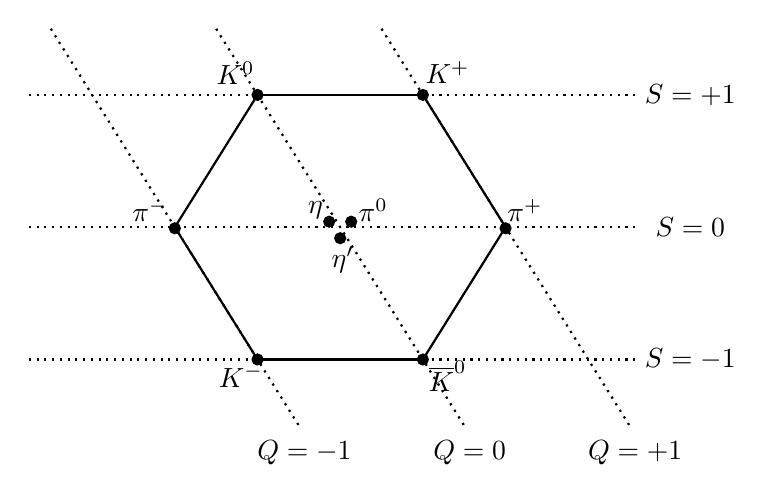
\begin{tikzpicture}
\begin{scope}[scale = 0.7] % overall scale 
%%
\begin{scope}[yscale = 1.2]
%%
%% hjelpelinjer
\draw    [thick, dotted]  (0,0)  --  (11,0);
\draw    [thick,dotted]  (0,2)  --  (11,2);
\draw    [thick, dotted]  (0,4)  --  (11,4);
\draw    [thick, dotted]  (0.4,5)  --  (4.9,-1);
\draw    [thick, dotted]  (0.4+3,5)  --  (4.9+3,-1);
\draw    [thick, dotted]  (0.4+6,5)  --  (4.9+6,-1);
%% hexagon
\begin{scope}[xshift = 0.05cm] % scope skifter og/eller skalerer innmaten
\draw    [thick]  (4.1,4)  --  (7.1,4);
\draw    [thick]  (4.1,4)  --  (2.6,2);
\draw    [thick]  (7.1,4)  --  (8.6,2);
\draw    [thick]  (4.1+4.5,2)  --  (2.6+4.5,0);
\draw    [thick]  (7.1-4.5,2)  --  (8.6-4.5,0);
\draw    [thick]  (4.1,0)  --  (7.1,0);
\end{scope}
\end{scope}
%% dots
\draw [fill] (4.15,0) circle [radius=0.1];
\draw [fill] (4.15+3,0) circle [radius=0.1];
\draw [fill] (4.15,4.8) circle [radius=0.1];
\draw [fill] (4.15+3,4.8) circle [radius=0.1];
\draw [fill] (2.65,2.38) circle [radius=0.1];
\draw [fill] (2.65+6,2.38) circle [radius=0.1];
\begin{scope}[xshift = -1.3cm,yshift = 0.7cm]
\draw [fill] (2.65+4.1,1.8) circle [radius=0.1];
\draw [fill] (2.65+4.5,1.8) circle [radius=0.1];
\draw [fill] (2.65+4.3,1.5) circle [radius=0.1];
\end{scope}
%% S,Q
\node at (12,0) {$S = -1$};
\node at (12,2.4) {$S = 0$};
\node at (12,4.8) {$S = +1$};
\node at (5,-1.7) {$Q = -1$};
\node at (5+3,-1.7) {$Q = 0$};
\node at (5+6,-1.7) {$Q = +1$};
%%partikler
\node at (4.15-0.3,0-0.3) {$K^-$};
\node at (4.15+3+0.45,0-0.3) {$\overline{K}^0$};
\node at (4.15-0.4,0-0.3 +5.5) {$K^0$};
\node at (4.15+3+0.45,0-0.3+5.5) {$K^+$};
\node at (2.2,2.7) {$\pi^-$};
\node at (2.2+6.8,2.7) {$\pi^+$};
\node at (5.2,2.7) {$\eta$};
\node at (6.25,2.7) {$\pi^0$};
\node at (5.7,1.8) {$\eta'$};
%%
%%
\end{scope} % overall scale end
\end{tikzpicture}
\caption{The pseudoscalar meson nonet}
\end{figure}


	
	We are now in a position to write an exponential representation for $U(x)$. This is an important step to note, as we here introduce the parameter that allows us to perform a perturbation approach later on. In other words, it is the first step in constructing our effective Lagrangian, and with it, the nucleon-nucleon potential. We define a set which maps spacetime to the $SU(N)$ group as
	
	\begin{equation}
		M_3 \equiv \left\{ U:M^4 \rightarrow SU(N)| U=\exp\big(i\frac{\phi}{F_0}\big), \phi\in M_2 \right\} \:,
	\end{equation}
	
	\noindent with $F_0$ being what we call the \emph{pion decay constant}. If we expand $U$, we get\footnote{The spacetime dependency lies in the matrices $\phi$.}
	
	\begin{equation}
		U = \mathds{1} + i\frac{\phi}{F_0} - \frac{\phi^2}{2F_0^2} + \ldots \:.
	\end{equation}
	
	\subsection{Effective Lagrangian}
	Since we have chiral symmetry, our Lagrangian is invariant under $U(x)$. Furthermore, we will get a Yang-Mills term and a mass term. The Yang-Mills term has the form:
	
	\begin{equation}
		\mathcal{L}_{\text{eff}} = \frac{F_0^2}{4}\Tr (\partial_\mu U \partial^\mu U) \:.
	\end{equation}
	
	For a local transform under a group $G$, which transforms as
	
	\begin{equation}
		U(x) \mapsto V_R(x)U(x)V_L^\dagger(x),
	\end{equation}
	
	\noindent the above kinetic term is no longer invariant. Instead, we need a covariant derivative $D$. In general, we may write
	
	\begin{equation}
		D_\mu A \equiv \partial_\mu A - ir_\mu A + iAl_\mu \:,
	\end{equation}
	
	\noindent where $l_\mu(x)$ and $r_\mu$ are external fields (remember the path integral formalism), and $A$ is any object which transforms as $V_RAV_L^\dagger$. The effective Lagrangian will contain infinitely many terms, with varying chiral order. Therefore, we here write the field-strength tensors needed to construct such high-order terms, although they will have no immediate use
	
	\begin{align}
		f_{R,\mu\nu} &\equiv \partial_\mu r_\nu - \partial_\nu r_\mu - i[r_\mu,r_\nu] \:, \\
		f_{L,\mu\nu} &\equiv \partial_\mu l_\nu - \partial_\nu l_\mu - i[l_\mu,l_\nu] \:,
	\end{align}
	
	There are now quite a few steps of analysis required to find which combinations of $l_\mu$, $r_\mu$, $U(X)$, and $D_\mu U(x)$ that preserve the conservation laws such as Lorentz invariance, charge conversion, parity conversion, etc, which we will only refer the reader to \cite{SchererSchingler12} from where most of the material presented here is found. Each combination will have with it a chiral order, which means that we may seperate the Lagrangian into ordered terms. The order of each object above is
	
	\begin{align}
		\begin{split}
		U &= \mathcal{O}(q^0) \:,\\
		D_\mu U &= \mathcal{O}(q^1) \:,\\
		r_\mu,l_\mu &= \mathcal{O}(q^1) \\
		f_{L/R,\mu\nu} &= \mathcal{O}(q^2) \:,\\
		\chi &= \mathcal{O}(q^2)\:,
		\end{split}
	\end{align}
	
	\noindent where $q$ is the meson momentum. We explain $\chi$ further below. We will end up with three terms, giving the lower order chiral effective Lagrangian:
	
	\begin{equation}
	\mathcal{L}_{\text{eff}}^{(2)} = \frac{F_0^2}{4}\Tr \left(D_\mu U (D^\mu U)^\dagger\right) + \frac{F_0^2}{4}\Tr (\chi U^\dagger + U\chi^\dagger) \:,
	\label{ChPtTh | eq | "lowest order meson Lagrangian"}
	\end{equation}
	
	\noindent where the superscript $(2)$ symbolises chiral order 2, the lower possible order, and $\chi \equiv 2B_0(s+ip)$ is a linear combination that transforms identically to $U$ under $G$, $C$ (charge conjugation), and $P$ (parity). The external fields $s$ and $p$ are scalar and pseudoscalar, respectively. $B_0$ is a physical constant, related to the scalar singlet quark condensate by \cite{SchererSchingler12}
	
	\begin{equation}
		3F_0^2B_0 = -\langle\bar{q}q\rangle_0 \:,
	\end{equation}
	
	Knowing we have spontaneous axial symmetry breaking, the mass term (ground-state term) must only be $SU(3)_V\times U(1)_V$ invariant.
	
	\subsubsection{Massive mesons}
	Now is a good time to see how meson mass terms naturally appear by reintroducing the quark masses. Firstly, the quark mass terms come in the shape of the quark mass matrix. As already mentioned, ChPT only works with the up, down, and strange quarks, so our matrix has three, non-zero values along the diagonal, i.e.
	
	\begin{equation}
		M = \begin{pmatrix}
		m_u & 0 & 0 \\
		0 & m_d & 0 \\
		0 & 0 & m_s
		\end{pmatrix}
	\end{equation}
	
	To the lower-order Lagrangian (equation (\ref{ChPtTh | eq | "lowest order meson Lagrangian"})), we have to add a term\footnote{This is the change in the Lagrangian that brings about an explicit symmetry breaking, such as discussed earlier.}
	
	\begin{equation}
		\mathcal{L}_{\text{sb}} = -\left( \bar{q}_R M q_L + \bar{q}_LMq_R \right) \:.
	\end{equation}
	
	\subsubsection{Renormalization}
	Finally we have an effective Lagrangian, at least to lowest chiral order. With it, we can start to calculate pion decay, pion-pion and Compton scattering. However, these are only tree-level diagrams. If we want to include loops in our calculations, we have to use renormalization to do so. In chapter 4 we discussed the main topics when it comes to renormalization, and now it is time to put that to use. Specifically, we will use dimensional regularization, as opposed to using a momentum cut-off $\Lambda$. Dimensional regularization means we keep the chiral algebra intact.\\
	
	To see how we would go about using dimensional regularization, we use an example \cite{SchererSchingler12} where we want to calculate a pion one-loop integral. From basic QFT, we know the integral is
	
	\begin{equation}
		I = \int\frac{d^4 k}{(2\pi)^4}\frac{i}{k^2 - m^2 + i\epsilon^+}
	\end{equation}
	
	\noindent where $\epsilon^+$ is a counter-clockwise infinitesimal rotation into the complex plane. As usual, we now let the number of dimensions be arbitrary, symbolised by $n$, giving
	
	\begin{equation}
	I_n = \mu^{4-n}\int\frac{d^n k}{(2\pi)^n}\frac{i}{k^2 - m^2 + i\epsilon^+}
	\end{equation}
	
	\noindent where $\mu$ is the 't Hooft renormalization scale, which is needed to maintain dimension 4 for all $n$. Furthermore, as the $\epsilon^+$ \emph{rotation} means it is best to work with spherical coordinates. In spherical coordinates, we replace the Minkowski integral over $n$-momentum space, parametrised with the Minkowski coordinates $\{l_i\}$ with the spherical integral over the angles $\{\theta_i\}$, the two coordinate sets related by, letting $l=\sqrt{l_1^2+l_2^2+\ldots +l_n^2}$
	
	\begin{align}
		\begin{split}
			l_1 &= l\cos(\theta_1) \\
			l_2 &= l\sin(\theta_1)\cos(\theta_2) \\
			l_3 &= l\sin(\theta_1)\sin(\theta_2)\cos(\theta_3) \\
			&\vdots \\
			l_{n-1} &= l\sin(\theta_1)\sin(\theta_2)\ldots\cos(\theta_{n-1}) \\
			l_{n} &= l\prod_{i=1}^{n-1}\sin(\theta_i)
		\end{split}
	\end{align}
	
	\noindent and the integral becomes:
	
	\begin{equation}
		\int d^nl = \int_0^\infty dl\:l^{n-1}\int_0^{2\pi}d\theta_{n-1}\int_0^\pi d\theta_{n-2}\:\sin(\theta_{n-2})  \ldots \int_0^\pi d\theta_1\:\sin^{n-2}(\theta_1)
	\end{equation}
	
	\noindent which integrates\footnote{Making use of $\int_0^\pi dx\:\sin^{m}(x) = \frac{\sqrt{\pi}\Gamma\big(\frac{m+1}{2}\big)}{\Gamma\big(\frac{m+2}{2}\big)}$} to
	
	\begin{align}
		\begin{split}
		\int_0^{2\pi}d\theta_{n-1} \ldots \int_0^\pi d\theta_1\:\sin^{n-2}(\theta_1) &= 2\pi^{\frac{n}{2}} \prod_{i=1}^{n-2} \frac{\Gamma\big(\frac{(n-2-i+1)+1}{2}\big)}{\Gamma\big(\frac{(n-2-i+1)+2}{2}\big)} \\
		&= 2\pi^{\frac{n}{2}} \prod_{i=1}^{n-2} \frac{\Gamma\big(\frac{n-i}{2}\big)}{\Gamma\big(\frac{(n-i+1}{2}\big)} \\
		&= 2\frac{\pi^{\frac{n}{2}}}{\Gamma\big(\frac{n}{2}\big)}
		\end{split}
	\end{align}
	
	We are left only with the integral over the "radius" $l$, such that:
	
	\begin{equation}
		I_n = \mu^{4-n}2\frac{\pi^{\frac{n}{2}}}{\Gamma\big(\frac{n}{2}\big)}\frac{1}{(2\pi)^n}\int_0^\infty \frac{l^{n-1}}{l^2 + m^2}
	\end{equation}
	
	By some non-trivial, intermediate steps, which we will omit here\footnote{See \cite{SchererSchingler12}, section 3.4.7, for details. The steps are few, but they require familiarity with complex analysis and analytic continuation. Vulgarized, analytic continuation is a method of extending a function beyond the space on which it is defined. A famous example where analytic continuation is used, is the Riemann zeta function.}, this becomes
	
	\begin{equation}
		I_n =\frac{m^2}{(4\pi)^2}\Big(\frac{4\pi\mu^2}{m^2}\Big)^{2-\frac{n}{2}}\Gamma\big(1-\frac{n}{2}\big)
	\end{equation}
	
	As we let $n\rightarrow4$, the $\Gamma$-function approaches a pole. Since the pole is related to the loop divergence, we must know how it grows.\\
	
	Using $\Gamma(z+1) = z\Gamma(z)$, and doing a Taylor expansion about $\epsilon = 4-n$ for the middle parenthesis above, we get \cite{SchererSchingler12}
	
	\begin{equation}
		I_n = \frac{m^2}{16\pi^2}\left[ R + \ln\Big(\frac{m^2}{\mu^2}\Big)\right] + \mathcal{O}(n-4)\:,\quad R=\frac{2}{n-4}-[\ln(4\pi) + \Gamma'(1)+1]
	\end{equation}
	
	As we see, the integral diverges as a simple pole due to the first term in $R$.
	
	\subsubsection{Massive pions}
	So far, we have only stated that the pseudoscalar currents fit perfectly with the pion tripled. However, while Goldstone bosons are massless, we know that pions have mass. How do we go about making the pions massive?\\
	
	The answer has already been given, although rather discretely, in the previous chapter. The divergences we encounter in the loop diagrams are removed in the renormalization group, in the sense that they are "swept under the carpet". It is believed that these divergences pop up due to our ignorance of the problem. Therefore, renormalization can be thought of as a systematic way to separate divergences, which our theory does not account for, from the finite terms, which our theory \emph{does} account for. As such, we turn to experiment or other theoretical, or numerical, schemes that determine the rescaled constants.\\
	
	The divergences are "scaled away" into constants, and these constants appear very much like the pions mass terms we have been wanting. Physics, sometimes, has a wonderous capability to seem like an impassable labyrinth, yet somehow we manage to get it right the first path we take.
	
	\subsection{Power counting}
	Now comes the time to see the practicality of all the lengthy mathematics we have covered so far, which is power counting. We have already mentioned Weinberg's theorem on the construction of effective Lagrangians. Therefore, we know that we have an infinitely long effective Lagrangian. It would be terribly inconvenient if we had to calculate all those terms, to see which are negligible and which are not. Fortunately, as we stated at the beginning of this section, we may group the Lagrangian terms into groups that increase, or \emph{scale}, with a certain order. Specifically, terms that have a certain chiral order.
	
	\begin{equation}
		\mathcal{L}_{\text{eff}} = \mathcal{L}^{(\Delta=2)} + \mathcal{L}^{(\Delta=4)} + \mathcal{L}^{(\Delta=6)} + \ldots\:,\quad \Delta:\:\text{chiral order}
	\end{equation}
	
	The chiral order is the number of Goldstone boson field derivatives and quark-mass terms. Since derivatives and mass-terms have to, separately, appear in even numbers per Lagrangian term, we only get even-powered terms\footnote{Quark masses are related to the chiral symmetry breaking scale by $M^2 \sim m_q$. A derivative corresponds to momentum in the Fourier transform, and because $p^2=m^2$ for on-shell fields, $p\sim M$. Furthermore, Lorentz invariance demands index summation, hence momentum always appears in twos. So we will always either have $p^2\sim M^2$ or $m_q\sim M^2$, giving even powers.}. This means that the first term only contains a pure mass-term, and a pure kinetic term. Of course, we already knew the lowest-order term was as such, because we have already derived it (eq \ref{ChPtTh | eq | "lowest order meson Lagrangian"}).\\
	
	We need a way to know which diagrams go into which $\mathcal{L}^{(i)}$. From the previous chapter, we know that power counting deals with that problem. At first, Weinberg suggested a power-counting formula
	
	\begin{equation}
		\Delta = nN_L - 2N_I + \sum_{k=1}^\infty 2kN_{2k}
	\end{equation}
	
	\noindent where
	
	\begin{align}
		\begin{split}
			n &:=\: \text{number of space-time dimensions} \\
			N_L &:=\: \text{number of independant loops} \\
			N_I &:=\: \text{number of internal Goldstone lines} \\
			N_{2k} &:=\: \text{number of vertices from $\mathcal{L}^{(2k)}$}
		\end{split}
	\end{align}
	
	\section{Baryon perturbation theory}
	For our purposes, we are more interested in working with baryons, rather than quarks. As already mentioned, ChPT works only below the chiral symmetry breaking scale, which is of order $\mathcal{O}(1\:\text{GeV})$. This has put a restriction on which quarks we can work with, and as such, which baryons we can work with. Baryons with masses less 
	than 1 GeV are the \emph{u-d-s baryon decuplet} and \emph{octet}. The baryon octet is drawn as shown in figure \ref{ChPtTh | fig | "baryon octet"}. 
	
	
\begin{figure}[h]\centering
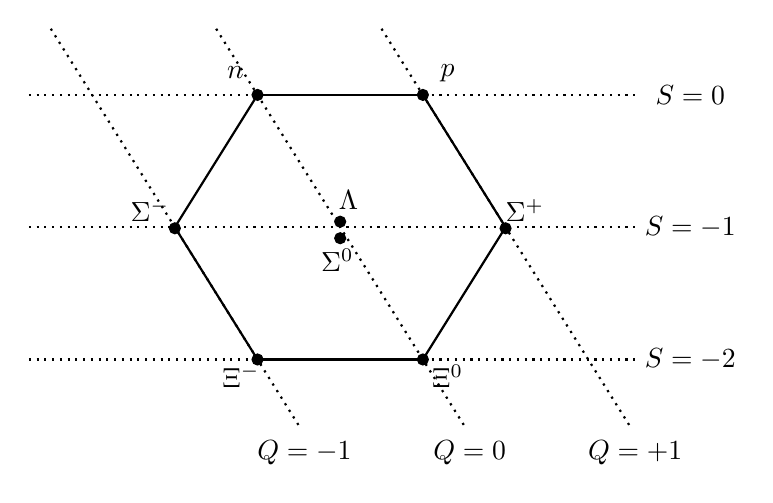
\begin{tikzpicture}
\begin{scope}[scale = 0.7] % overall scale 
%%
\begin{scope}[yscale = 1.2]
%%
%% hjelpelinjer
\draw    [thick, dotted]  (0,0)  --  (11,0);
\draw    [thick,dotted]  (0,2)  --  (11,2);
\draw    [thick, dotted]  (0,4)  --  (11,4);
\draw    [thick, dotted]  (0.4,5)  --  (4.9,-1);
\draw    [thick, dotted]  (0.4+3,5)  --  (4.9+3,-1);
\draw    [thick, dotted]  (0.4+6,5)  --  (4.9+6,-1);
%% hexagon
\begin{scope}[xshift = 0.05cm] % scope skifter og/eller skalerer innmaten
\draw    [thick]  (4.1,4)  --  (7.1,4);
\draw    [thick]  (4.1,4)  --  (2.6,2);
\draw    [thick]  (7.1,4)  --  (8.6,2);
\draw    [thick]  (4.1+4.5,2)  --  (2.6+4.5,0);
\draw    [thick]  (7.1-4.5,2)  --  (8.6-4.5,0);
\draw    [thick]  (4.1,0)  --  (7.1,0);
\end{scope}
\end{scope}
%% dots
\draw [fill] (4.15,0) circle [radius=0.1];
\draw [fill] (4.15+3,0) circle [radius=0.1];
\draw [fill] (4.15,4.8) circle [radius=0.1];
\draw [fill] (4.15+3,4.8) circle [radius=0.1];
\draw [fill] (2.65,2.38) circle [radius=0.1];
\draw [fill] (2.65+6,2.38) circle [radius=0.1];
\begin{scope}[xshift = -1.3cm,yshift = 0.7cm]
\draw [fill] (2.65+4.3,1.8) circle [radius=0.1];
%\draw [fill] (2.65+4.5,1.8) circle [radius=0.1];
\draw [fill] (2.65+4.3,1.5) circle [radius=0.1];
\end{scope}
%% S,Q
\node at (12,0) {$S = -2$};
\node at (12,2.4) {$S = -1$};
\node at (12,4.8) {$S = 0$};
\node at (5,-1.7) {$Q = -1$};
\node at (5+3,-1.7) {$Q = 0$};
\node at (5+6,-1.7) {$Q = +1$};
%%partikler
\node at (4.15-0.3,0-0.3) {$\Xi^-$};
\node at (4.15+3+0.45,0-0.3) {$\Xi^0$};
\node at (4.15-0.4,0-0.3 +5.5) {$n$};
\node at (4.15+3+0.45,0-0.3+5.5) {$p$};
\node at (2.2,2.7) {$\Sigma^-$};
\node at (2.2+6.8,2.7) {$\Sigma^+$};
\node at (5.6,1.8) {$\Sigma^0$};
\node at (5.8,2.9) {$\Lambda$};
%\node at (5.7,1.8) {$\eta'$};
%%
%%
\end{scope} % overall scale end
\end{tikzpicture}
\caption{The spin-$\frac{1}{2}$ baryon octet}
\label{ChPtTh | fig | "baryon octet"}
\end{figure}
	
	As a reminder, we note that the decuplet give the quantum numbers of all spin-$\frac{3}{2}$ baryons made of a selection of the $u$, $d$, and $s$ quarks. The octet gives the quantum numbers of all spin-$\frac{1}{2}$ baryons, taken from the same selection. Of course, we are only interested in interactions that occur in nuclear matter, which is made of stable neutrons (udd) and protons (uud). Since protons and neutrons are spin-$\frac{1}{2}$ particles\footnote{It is easy to remember they are spin-$\frac{1}{2}$ and not spin-$\frac{3}{2}$, due to 3 facts; higher spin usually means higher energies, all atoms are made of protons and neutrons, and nature tends to be as least energetic as possible.}, we need to work with the octet field matrix. We may arrange the 8 baryon fields in a traceless matrix:
	
	\begin{equation}
		B = \sum_{a=1}^8 \frac{B_a\lambda_a}{\sqrt{2}} = \begin{pmatrix}
		\frac{1}{\sqrt{2}}\Sigma^0 + \frac{1}{\sqrt{2}}\Lambda & \Sigma^+ & p \\
		\Sigma^- & -\frac{1}{\sqrt{2}}\Sigma^0 + \frac{1}{6}\Lambda & n \\
		\Xi^- & \Xi^0 & -\frac{2}{\sqrt{6}}\Lambda \:.
		\end{pmatrix}
	\end{equation}
	
	
	
	\begin{figure}[h]
		\centering
		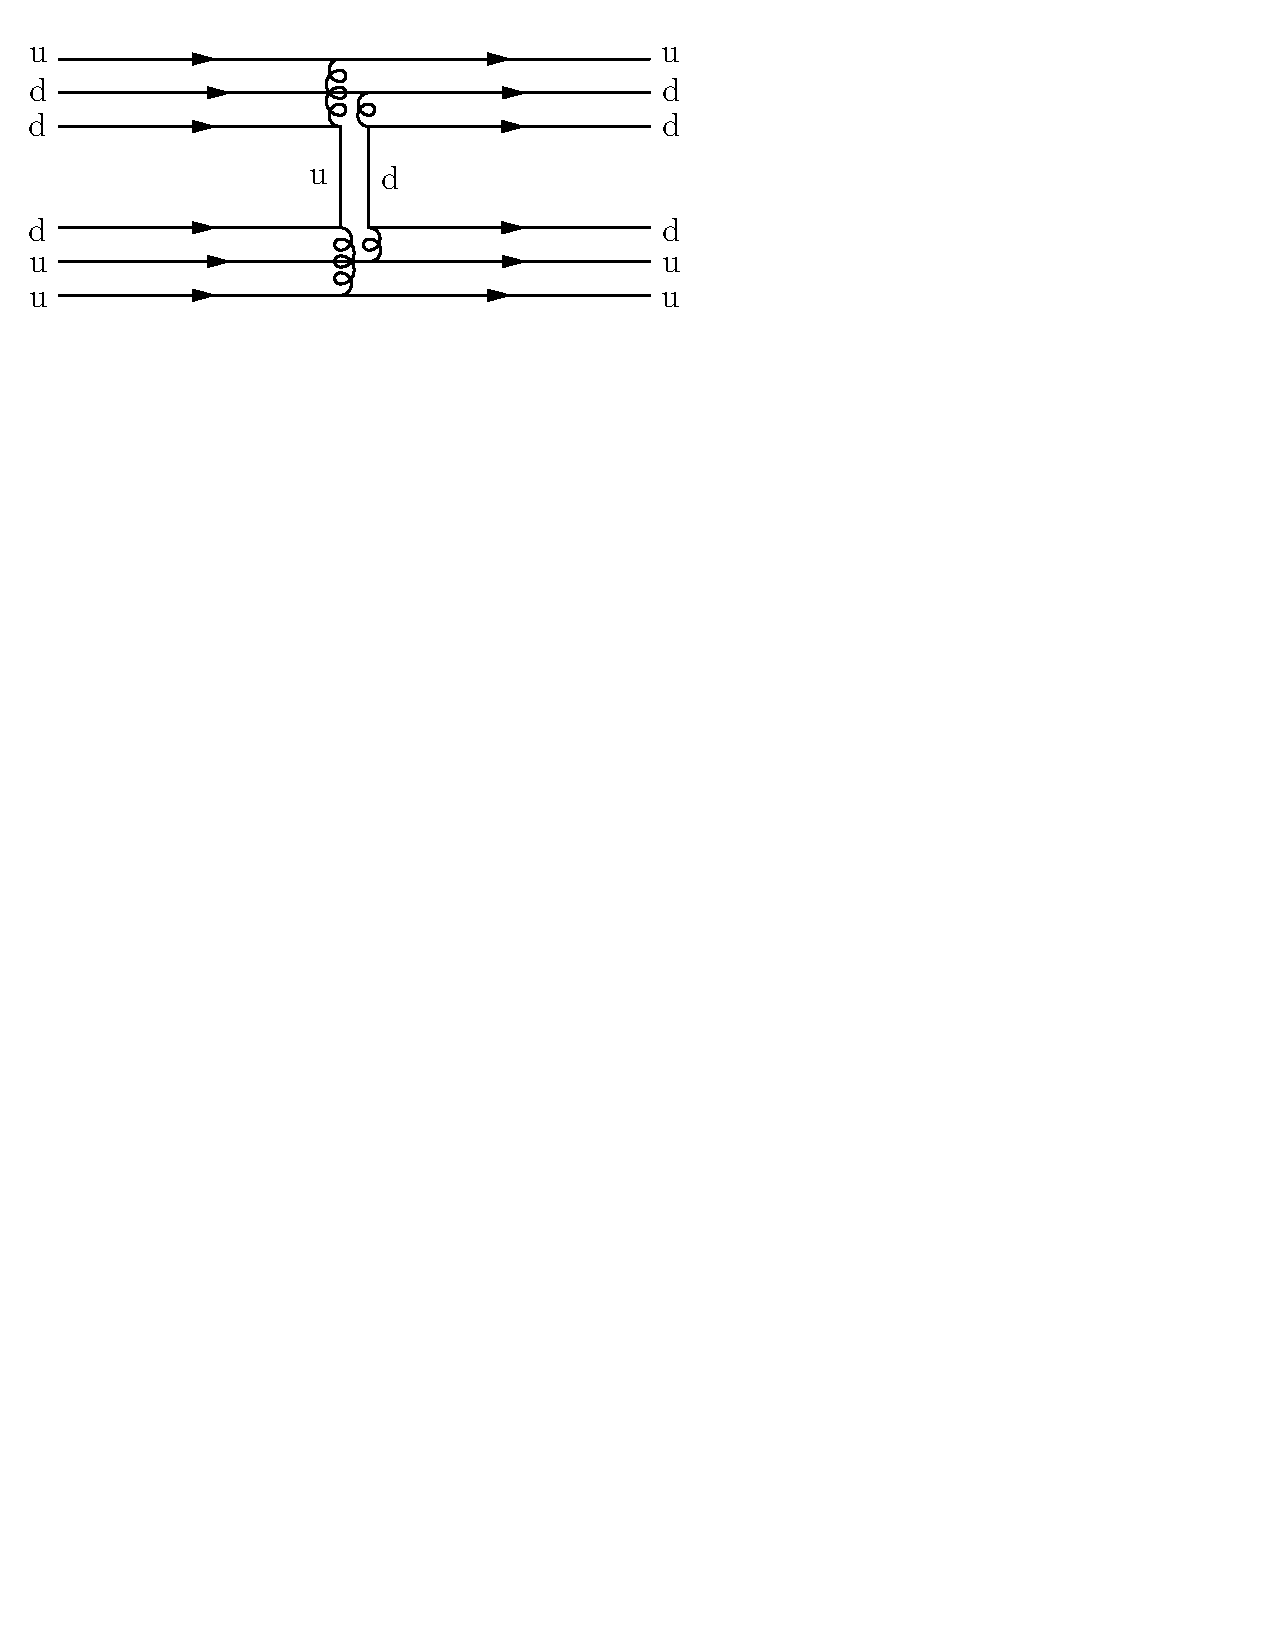
\includegraphics[trim={0.5cm 22cm 10cm 0cm},width=0.5\textwidth]{Figures/Pion_exch.pdf}
		\caption{Fewest vertices possible for proton-neutron pion exchange}
		\label{fey:1}
	\end{figure}
	
	\subsection{Heavy baryon formalism}
	Treating baryons relativistically with chiral perturbation theory is tricky, since the time derivative of the baryon field gives a factor of $E$ (the energy), which has the same size as the mass $M$ ($E\simeq M$). Since $M\simeq\Lambda_\chi$, we find that perturbation in these variables puts us right back where we started with an non-perturbative theory. Fortunately, there is a workaround that deals with this. If the baryons are treated as static sources\footnote{This means that the baryons' positions are not much altered by the strong interaction.}, then it means that the baryons trade very little momenta by pion interactions. Below we shall outline how this is done mathematically.\\
	
	We are moving into harder and harder topics to explain from first principles. Therefore, rather than explain thoroughly the theory behind heavy baryon expansions\footnote{We also write HBChPT: Heavy Baryon Chiral Perturbation Theory.}, we shall present a quicker introduction. We shall follow the steps as presented in \cite{MachleidtEntem11}.\\
	
	The heavy baryons can have their 4-momenta split as
	
	\begin{equation}
		p^\mu = Mv^\mu + l^\mu\:,
	\end{equation}
	
	\noindent where $v^\mu$ is the 4-momentum, satisfying $v^2 = 1$, and $l^\mu$ is a small residual such that $v\cdot \ll M$. We then define velocity-dependent fields $N$ and $h$,
	
	\begin{align}
		\begin{split}
		N &\equiv e^{iMv\cdot x}P_v^+\Psi\:, \\
		h &\equiv e^{iMv\cdot x}P_v^-\Psi\:, \\
		\end{split}
	\end{align}
	
	\noindent where
	
	\begin{equation}
		P_v^\pm = \frac{1\pm\gamma_\nu v^\nu}{2}\:,
	\end{equation}
	
	\noindent are projection operators. The baryon spinor field can now be written
	
	\begin{equation}
		\Psi = e^{-iMv\cdot x}(N+h)
	\end{equation}
	
	The exponential factor in $N$ and $h$ means that all dependence on $M$ disappears from the kinematic baryon terms in the Lagrangian.\\
	
	Going back to the leading order Lagrangian ($\mathcal{L}_{\pi N}^{(1)}$),
	
	\begin{equation}
	\mathcal{L}_{\pi N}^{(1)} = \overbar{\Psi}\left( i\gamma^\mu D_\mu - M + \frac{g_A}{2}\gamma^\mu\gamma_5u_\mu \right)\Psi \:,
	\end{equation}
	
	\noindent it is possible to derive the heavy baryon, leading order Lagrangian ($\widehat{\mathcal{L}}_{\pi N}^{(1)}$) by using the $N$ and $h$ decomposition of $\Psi$ (\cite{MachleidtEntem11},\cite{SchererSchingler12});
	
	\begin{equation}
		\widehat{\mathcal{L}}_{\pi N}^{(1)} = \overbar{N}\left( iD^0 + \frac{g_A}{2}\bm{\sigma}\cdot \bm{u} \right)N \:,
		\label{ChPtTh | eq | "heavy baryon 1st order L"}
	\end{equation}
	
	\noindent plus all corrections that scale as $1/M$. The covariant derivative $D_0$ can be expanded in powers of pion fields, meaning that we can express equation (\ref{ChPtTh | eq | "heavy baryon 1st order L"}) as an expansion as well, \cite{MachleidtEntem11}
	
	\begin{align}
		\begin{split}
		\widehat{\mathcal{L}}_{\pi N}^{(1)} = &\overbar{N}\Big\{ i\partial^0 -\frac{1}{4f_\pi^2}\bm{\tau}\cdot(\bm{\pi}\times\partial_0\bm{\pi}) - \frac{g_A}{2f_\pi}\bm{\tau}\cdot(\bm{\sigma}\cdot\nabla)\bm{\pi}\\
		&+ \frac{g_A(4\alpha-1)}{4f_\pi^3}(\bm{\tau}\cdot\bm{\pi})\left[\bm{\pi}\cdot(\bm{\sigma}\cdot\nabla)\bm{\pi}\right] + \frac{g_A\alpha}{2f_\pi^3}\bm{\pi}^2\left[\bm{\tau}\cdot(\bm{\sigma}\cdot\nabla)\bm{\pi}\right] \Big)N + \mathcal{O}(\bm{\pi}^4) \:.
		\end{split}
	\end{align}
	
	Higher order Lagrangians can be derived similarly, and will depend on the effective constants $c_i$, see \cite{MachleidtEntem11}.
	
	
	\newpage
	\chapter{Interacting Nuclear Matter}
	\label{Int.Nucl.Mat.}
	\epigraph{\textit{Ordo ab chao}}{- Masonic motto}
	
	The theory of nuclear forces started in 1935, with Hideki Yukawa's paper \cite{Yukawa35} on boson force carriers within nuclei. His model had much success when the least massive meson, the pion, was measured in 1947, with about the same mass as Yukawa had predicted. Later on, in the 1950's, people started making potentials with one-pion exchanges. These new potentials fitted very well with NN scattering experiments, providing insight into the deuteron, thus furthering the understanding of the angluar momentum dependant force of the strong interaction.  Unfortunately, multi-pion exchanges did not have the same success and remained a problem. It was solved the following decade after much theoretical work with dispersion and field theory were used, and is when potentials such as Paris and Bonn were proposed. Following the discovery of QCD, the meson theories seemed disjoint from their constituents due to the non-perturbative nature of low-energy QCD. It was not until Weinberg's 1979 paper \cite{Weinberg79} on effective field theories that meson theories and QCD overlapped, which we already know to be chiral perturbation theory. We refer the reader to \cite{MachleidtEntem11} for a more rigorous review on the history of the nuclear force.\\
	
	So far we have been entirely dedicated to the development of chiral perturbation theory. However, we have not mentioned nuclear structure theory at all, which is very important when it comes to understanding the nature of the nuclear force.  %However, this is far from the only way to make potentials describing nuclear matter. Here, we shall present alternate approaches to nuclear interactions, as well as give a more detailed description of how to go from having a QFT to a potential that we can put into the Schr\"odinger equation.
	
	\section{Interacting nucleons and nuclei}
	Before we discuss properties of nuclear forces, it would be best to briefly review partial wave expansions and the phenomenology of nuclear forces.
	
	\subsubsection{Partial wave analysis}
	In introductory quantum mechanics, we tend to get a thorough introduction to partial wave expansion. Here we shall give a short repetition of the topic. When working in momentum space, we will have a factor $e^{i\bm{k}\cdot\bm{r}}$. Such an exponential function can be written in terms of Bessel functions;
	
	\begin{equation}
		e^{i\bm{k}\cdot\bm{r}} = \sum_{l=0}^{\infty} \sqrt{4\pi(2l+1)}i^lj_l(kr)Y_{l0}
	\end{equation}
	
	Each $l$ is an angular momentum \emph{partial wave}, hence the name.
	
	\subsubsection{Centre of mass system}
	There is little point in working in any other system than the centre of mass (CoM) system when working with the two-body force. As we already know, we can then work with the total momentum,
	
	\begin{equation}
		\bm{K} = \sum_{i=1}^A \bm{k}_i\:,
	\end{equation}
	
	\noindent and relative momentum,
	
	\begin{equation}
		\bm{k}_{ij} = \frac{1}{2}(\bm{k}_i - \bm{k}_j) \:
	\end{equation}
	
	Furthermore, we may separate the Schr\"odinger equation into a radial and angular part. We now split the angular momentum into a CoM momentum term and a relative momentum term, i.e.
	
	\begin{equation}
		\hat{l}_1 + \hat{l}_2 = \hat{l} + \hat{L}\:,
	\end{equation}
	
	where $\hat{l}$ is the relative and $\hat{L}$ the CoM angular momentum. The total angular momentum is now
	
	\begin{equation}
		\hat{J} = \hat{l} + \hat{L} + \hat{S}\:,
	\end{equation}
	
	\noindent where $S$ is the total spin. The total angular momentum to the relative motion is then
	
	\begin{equation}
		\mathcal{J} = \hat{l} + \hat{S}\:,
	\end{equation}
	
	\noindent since spin is not a function of space. The reader might be wondering what all this rewriting is good for. With these quantities, we can quite easily, by using the spin statistics theorem, find out which two-particle partial waves exist for the two-nucleon system. If we assume isospin symmetry, and $S=0$, then the only possible s-waves\footnote{Remember that s-waves are spherically symmetric functions.} that preserve anti-symmetry have a total isospin of one ($T=1$). The projections for $T$ are $T_z=\{-1,0,1\}$, and as such either $|nn\rangle$, $|pn\rangle$, or $|pp\rangle$ can exist in an s-wave. This is just one example, but it is not difficult to find quantum number combinations by continuing to use these types of symmetry arguments. In table \ref{On int nucl | table | "spins for two-body states up to f-waves"}, the possible partial waves per two-nucleon state are listed up to the f-waves \cite{phy981}. All it really comes down to is whether or not the spatial part of the wave function is symmetric (s,p,d,f,$\ldots$,-waves), which restricts the value of $J$, $l$, and $S$, which in turn decides the value of $T$, and $T$ determines which two-nucleon states are allowed.
	
	\begin{table}[h]
		\centering
		\captionsetup{width=.8\textwidth}
		\caption{\cite{phy981} Angular quantum numbers for states up to $f$-waves. Not all nucleon-nucleon two-body states can be achieved. We point out that $|\bm{1}-\bm{S}|\leq|\bm{J}|\leq|\bm{1}+\bm{S}|$}
		\begin{tabular}{cccccccc}
			$^{2S+1}l_J$ & $J$ & $S$ & $S$ & $T$ & $|pp\rangle$ & $|pn\rangle$ & $|nn\rangle$ \\
			$^1S_0$ & 0 & 0 & 0 & 1 & \checkmark & \checkmark & \checkmark \\
			$^3S_1$ & 1 & 0 & 1 & 0 & \text{\sffamily X} & \checkmark & \text{\sffamily X} \\
			$^3P_0$ & 0 & 1 & 1 & 1 & \checkmark & \checkmark & \checkmark \\
			$^1P_1$ & 1 & 1 & 0 & 0 & \text{\sffamily X} & \checkmark & \text{\sffamily X} \\
			$^3P_1$ & 1 & 1 & 1 & 1 & \checkmark & \checkmark & \checkmark \\
			$^3P_2$ & 2 & 1 & 1 & 1 & \checkmark & \checkmark & \checkmark \\
			$^3D_1$ & 1 & 2 & 0 & 0 & \text{\sffamily X} & \checkmark & \text{\sffamily X} \\
			$^3F_2$ & 2 & 3 & 1 & 1 & \checkmark & \checkmark & \checkmark \\
		\end{tabular}
		\label{On int nucl | table | "spins for two-body states up to f-waves"}
	\end{table}
	
	\subsubsection{Tensor force}
	The nuclear force is not just a radial-dependant interaction, but also has a spin-dependant interaction which we call the \emph{tensor force}. It is given by \cite{phy981}
	
	\begin{equation}
		S_{12}(\hat{r}) = \frac{3}{r^2}(\sigma_1\cdot\bm{r})(\sigma_2\cdot\bm{r}) - \sigma_1\cdot\sigma_2 \:,
	\end{equation}
	
	\noindent where $\bm{r}$ is the relative distance and $\sigma_i$ are the Pauli matrices: $\{\sigma_x,\:\sigma_y,\:\sigma_z\}$. From quantum mechanics, we know that the expectation value of spin, in the two-body system, is
	
	\begin{equation}
		\langle\sigma_1\cdot\sigma_2\rangle = 2(S^2 - s_1^2 - s_2^2) = 2S(S+1) - 3
	\end{equation}
	
	\subsection{Characteristics of nuclear forces}
	The nucleon-nucleon (NN) force has a number of characteristic properties \cite{phy981}:
	
	\begin{itemize}
		\item Firstly, the deuteron\footnote{Deuterium is one of the two stable isotopes of hydrogen. It has a proton and neutron in its core.} has spin $J^\pi = 1^+$, which indicates that there is an attractive force between the proton and the neutron for the $^3S_1$ partial wave. Furthermore, the NN force is attractive for the proton-proton partial wave $^1S_0$, as is known from inference between Coulomb and nuclear scattering. \\
		\item It is spin dependent, because the scattering lengths are different for the triplet and singlet states.\\
		\item It is \emph{nearly} charge-independent. Any two nucleons in some two-body state will experience almost the same force. However, since charge and isospin symmetry are slightly broken, the neutron-neutron, proton-proton, and neutron-neutron forces are different, for the same two-body states.
	\end{itemize} 
	
	\section{The chiral effective Lagrangian}
	Using the chiral perturbation formalism of the previous chapter, the effective Lagrangian for nuclear systems can be written:
	
	\begin{equation}
		\mathcal{L}_{\text{eff}} = \underbrace{\mathcal{L}_{\pi\pi}}_{N^0} + \underbrace{\mathcal{L}_{\pi N}}_{N^1} + \underbrace{\mathcal{L}_{NN} + \mathcal{L}_{\pi NN} + \mathcal{L}_{\pi\pi NN} + \ldots}_{N^2} + \underbrace{\mathcal{L}_{NNN} + \mathcal{\mathcal{L}}_{\pi NNN} + \ldots}_{N^3} + \underbrace{\ldots}_{N^{n\geq 4}}
	\end{equation}
	
	As one can see, the Lagrangian is infinitely long, but this is no different than what is seen in perturbative quantum field theory, as we ignore effects above a certain order. The classification of orders, given by the so-called index of interaction,
	
	\begin{equation}
		\Delta \equiv d + \frac{n}{2} - 2,
	\end{equation}
	
	\noindent where $d$ is the number of derivatives or pion-masses and $n$ is the number of nucleon fields, allows us to rewrite the Lagrangian as
	
	\begin{equation}
		\mathcal{L} = \mathcal{L}^{\Delta = 0} + \mathcal{L}^{\Delta = 1} + \mathcal{L}^{\Delta = 2} + \mathcal{L}^{\Delta = 4} + \ldots
	\end{equation}
	
	This is deceptively simple-looking. Each term here is quite complicated, and many papers have been written on the topic of their derivation. An excellent account of the derivations, as well as ChPT in general, can be read in \cite{MachleidtEntem11}.  Performing naive dimensional analysis, where we assign a power to each appearance of a pion mass term or momentum\footnote{Either nucleon 3-momentum or pion 4-momentum.}, Weinberg showed that the power of an irreducible Feynman diagram will satisfy
	
	\begin{equation}
		\nu_W = 4-A-2C + 2L + \sum_i\Delta_i\:,
	\end{equation}
	
	\noindent where $A$ is the number of nucleon lines, $C$ the number of separately connected pieces, and $L$ is the number of loops. The formula works for all cases of $A\leq2$, but problems may arise for $A>2$. Therefore, it is now more common to use the modified version for $A\geq 2$:
	
	\begin{equation}
		\nu = -2+2A-2C+2L+\sum_i\Delta_i \:.
	\end{equation}
	
	\begin{figure}
	\centering
	\captionsetup{width=.8\textwidth}
\begin{tikzpicture}
\begin{scope}[scale = 0.7] % overall scale 
%%
\begin{scope}[yscale = 1.2]
%%
%% text
\begin{scope}[xshift = 0.05cm]
\node (NN) at (6.4cm,5cm) {NN};
\end{scope}
\begin{scope}[xshift = 10.05cm]
\node (NNN) at (6.4cm,5cm) {NNN};
\end{scope}
\begin{scope}[xshift = 0.05cm, yshift=2.75cm]
\node (LO) at (0cm,0.25cm) {$\underset{\nu=0}{\text{LO}}$};
\end{scope}
\begin{scope}[xshift = 0.05cm, yshift=-1.5cm]
\node (NLO) at (0cm,0.25cm) {$\underset{\nu=1}{\text{NLO}}$};
\end{scope}
\begin{scope}[xshift = 0.05cm, yshift=-7cm]
\node (NNLO) at (0cm,0.25cm) {$\underset{\nu=2}{\text{NNLO}}$};
\end{scope}
%%
%% NN interactions
%% LO
\begin{scope}[xshift = 0.05cm] % scope skifter og/eller skalerer innmaten
\draw   [thick]		(4.1,4)	 --	 (2.6,2);
\draw	[thick]		(2.6,4)	 --  (4.1,2);
\draw	[fill] 		(3.35,3) circle [radius=0.1];
\end{scope}
%
\begin{scope}[xshift = 3.05cm]
\draw   [thick]		(4.1,4)	 --	 (4.1,2);
\draw	[thick]		(2.6,4)	 --  (2.6,2);
\draw	[thick, dashed]		(2.6,3)	 --  (4.1,3);
\draw	[fill] 		(2.6,3) circle [radius=0.1];
\draw	[fill] 		(4.1,3) circle [radius=0.1];
\end{scope}
%
%% NLO
\begin{scope}[xshift = 0.05cm, yshift = -3.00cm]
\draw   [thick]		(4.1,4)	 --	 (2.6,2);
\draw	[thick]		(2.6,4)	 --  (4.1,2);
\filldraw [draw=black] (3.35-0.15,3-0.15) rectangle ++(0.3,0.3);
\end{scope}
%
\begin{scope}[xshift = 3.05cm, yshift = -3.00cm]
\draw   [thick]		(4.1,4)	 --	 (4.1,2);
\draw	[thick]		(2.6,4)	 --  (2.6,2);
\draw	[fill] 		(2.6,3) circle [radius=0.1];
\node (B) at (2.6,3) {};
\draw	[fill] 		(4.1,3) circle [radius=0.1];
\node (C) at (4.1,3) {};
\path	[thick, dashed, bend left]	(B)	 edge  (C);
\path	[thick, dashed, bend right]	(B)	 edge  (C);
\end{scope}
%
\begin{scope}[xshift = 6.05cm, yshift = -3.00cm]
\draw   [thick]		(4.1,4)	 --	 (4.1,2);
\draw	[thick]		(2.6,4)	 --  (2.6,2);
\draw	[thick, dashed]		(2.6,3)	 --  (4.1,2.5);
\draw	[thick, dashed]		(2.6,3)	 --  (4.1,3.5);
\draw	[fill] 		(2.6,3) circle [radius=0.1];
\draw	[fill] 		(4.1,2.5) circle [radius=0.1];
\draw	[fill] 		(4.1,3.5) circle [radius=0.1];
\end{scope}
%
\begin{scope}[xshift = 0.05cm, yshift = -5.50cm]
\draw   [thick]		(4.1,4)	 --	 (4.1,2);
\draw	[thick]		(2.6,4)	 --  (2.6,2);
\draw	[thick, dashed]		(4.1,3)	 --  (2.6,2.5);
\draw	[thick, dashed]		(4.1,3)	 --  (2.6,3.5);
\draw	[fill] 		(2.6,2.5) circle [radius=0.1];
\draw	[fill] 		(2.6,3.5) circle [radius=0.1];
\draw	[fill] 		(4.1,3.0) circle [radius=0.1];
\end{scope}
%
\begin{scope}[xshift = 3.05cm, yshift = -5.50cm]
\draw   [thick]		(4.1,4)	 --	 (4.1,2);
\draw	[thick]		(2.6,4)	 --  (2.6,2);
\draw	[thick, dashed]		(4.1,2.5)	 --  (2.6,2.5);
\draw	[thick, dashed]		(4.1,3.5)	 --  (2.6,3.5);
\draw	[fill] 		(2.6,2.5) circle [radius=0.1];
\draw	[fill] 		(2.6,3.5) circle [radius=0.1];
\draw	[fill] 		(4.1,2.5) circle [radius=0.1];
\draw	[fill] 		(4.1,3.5) circle [radius=0.1];
\end{scope}
%%
\begin{scope}[xshift = 6.05cm, yshift = -5.50cm]
\draw   [thick]		(4.1,4)	 --	 (4.1,2);
\draw	[thick]		(2.6,4)	 --  (2.6,2);
\draw	[thick, dashed]		(4.1,2.5)	 --  (2.6,3.5);
\draw	[thick, dashed]		(4.1,3.5)	 --  (2.6,2.5);
\draw	[fill] 		(2.6,2.5) circle [radius=0.1];
\draw	[fill] 		(4.1,3.5) circle [radius=0.1];
\draw	[fill] 		(4.1,2.5) circle [radius=0.1];
\draw	[fill] 		(2.6,3.5) circle [radius=0.1];
\end{scope}
%
%% NNLO
\begin{scope}[xshift = 0.05cm, yshift = -8.50cm]
\draw   [thick]		(4.1,4)	 --	 (4.1,2);
\draw	[thick]		(2.6,4)	 --  (2.6,2);
\node (B) at (2.6,3) {};
\begin{scope}[xshift = 2.6cm, yshift = 3cm]
\filldraw [draw=black,rotate=45] (-0.15,-0.15) rectangle ++(0.3,0.3);
\end{scope}
\draw	[fill] 		(4.1,3) circle [radius=0.1];
\node (C) at (4.1,3) {};
\path	[thick, dashed, bend left]	(B)	 edge  (C);
\path	[thick, dashed, bend right]	(B)	 edge  (C);
\end{scope}
%
\begin{scope}[xshift = 3.05cm, yshift = -8.50cm]
\draw   [thick]		(4.1,4)	 --	 (4.1,2);
\draw	[thick]		(2.6,4)	 --  (2.6,2);
\draw	[thick, dashed]		(2.6,3)	 --  (4.1,2.5);
\draw	[thick, dashed]		(2.6,3)	 --  (4.1,3.5);
\draw	[fill] 		(2.6,3) circle [radius=0.1];
\draw	[fill] 		(4.1,2.5) circle [radius=0.1];
\draw	[fill] 		(4.1,3.5) circle [radius=0.1];
\end{scope}
%
\begin{scope}[xshift = 6.05cm, yshift = -8.50cm]
\draw   [thick]		(4.1,4)	 --	 (4.1,2);
\draw	[thick]		(2.6,4)	 --  (2.6,2);
\draw	[thick, dashed]		(4.1,3)	 --  (2.6,2.5);
\draw	[thick, dashed]		(4.1,3)	 --  (2.6,3.5);
\draw	[fill] 		(2.6,2.5) circle [radius=0.1];
\draw	[fill] 		(2.6,3.5) circle [radius=0.1];
\draw	[fill] 		(4.1,3.0) circle [radius=0.1];
\end{scope}
%
\begin{scope}[xshift = 0.05cm, yshift = -11.00cm]
\draw   [thick]		(4.1,4)	 --	 (4.1,2);
\draw	[thick]		(2.6,4)	 --  (2.6,2);
\node (B) at (4.1,3) {};
\draw	[fill] 		(2.6,3) circle [radius=0.1];
\node (C) at (2.6,3) {};
\begin{scope}[xshift = 4.1cm, yshift = 3cm]
\filldraw [draw=black,rotate=45] (-0.15,-0.15) rectangle ++(0.3,0.3);
\end{scope}
\path	[thick, dashed, bend left]	(B)	 edge  (C);
\path	[thick, dashed, bend right]	(B)	 edge  (C);
\end{scope}
%
%% NNN interactions
%% NNLO
\begin{scope}[xshift = 10.05cm, yshift = -8.50cm]
\draw   [thick]		(4.1,4)	 --	 (2.6,2);
\draw	[thick]		(2.6,4)	 --  (4.1,2);
\draw	[thick]		(3.35,4) --  (3.35,2);
\node (B) at (3.35,3) {};
\begin{scope}[xshift = 3.35cm, yshift = 3cm]
\filldraw [draw=black,rotate=45] (-0.15,-0.15) rectangle ++(0.3,0.3);
\end{scope}
\end{scope}
%
\begin{scope}[xshift = 13.05cm, yshift = -8.50cm]
\draw	[thick]		(2.6,4) --  (2.6,2);
\draw   [thick]		(4.1,4)	 --	 (3.2,2);
\draw	[thick]		(3.2,4)	 --  (4.1,2);
\draw	[thick,dashed]		(2.6,3)	 --  (3.65,3);
\draw	[fill] 		(2.6,3) circle [radius=0.1];
\node (C) at (3.65,3) {};
\begin{scope}[xshift = 3.65cm, yshift = 3cm]
\filldraw [draw=black,rotate=45] (-0.15,-0.15) rectangle ++(0.3,0.3);
\end{scope}
\end{scope}
%
\begin{scope}[xshift = 16.05cm, yshift = -8.50cm]
\draw   [thick]		(4.1,4)	 --	 (4.1,2);
\draw	[thick]		(3.35,4)	 --  (3.35,2);
\draw	[thick]		(2.6,4)	 --  (2.6,2);
\draw	[thick, dashed]		(2.6,3)	 --  (4.1,3);
\draw	[fill] 		(2.6,3) circle [radius=0.1];
\draw	[fill] 		(4.1,3) circle [radius=0.1];
\node (B) at (3.35,3) {};
\begin{scope}[xshift = 3.35cm, yshift = 3cm]
\filldraw [draw=black,rotate=45] (-0.15,-0.15) rectangle ++(0.3,0.3);
\end{scope}
\end{scope}
%
%%
%%
\end{scope}
\end{scope} % overall scale end
\end{tikzpicture}
\caption{The leading order, next-to-leading order, and next-to-next-to-leading order interaction diagrams for the two- and three-nucleon case \cite{CarlssonEtAl16}. The solid lines represent nucleons, while the dashed lines are pions. The circle, diamond, and square vertices are of chiral order $\Delta = 0,1,2$, respectively.}
\end{figure}
	
	\subsection{Two-nucleon interactions}
	The two-body nucleon-nucleon (NN) interaction is found by perturbation in orders of pion momentum. This means that the more pions we include in our Feynman diagrams, the smaller that diagram's contribution is to the effective potential. Below, we repeat the expressions of \cite{MachleidtEntem11} for the nucleon-nucleon force. There are two levels to how we may write the interaction. Firstly, by how many pions take part in the interaction, and secondly by the momentum scale. Therefore, we get the pion number terms
	
	\begin{equation}
		V_{\pi} = V_{1\pi}+V_{2\pi}+V_{3\pi}+\ldots \:,
	\end{equation}
	
	\noindent where each term has the momentum expansion
	
	\begin{align}
		V_{1\pi} &= V_{1\pi}^{(0)} + V_{1\pi}^{(2)} + V_{1\pi}^{(3)} +\ldots \:,\\
		V_{2\pi} &= V_{2\pi}^{(2)} + V_{2\pi}^{(3)} + V_{2\pi}^{(4)} +\ldots \:,\\
		V_{3\pi} &= V_{3\pi}^{(4)} + V_{3\pi}^{(5)} + V_{3\pi}^{(6)} +\ldots \:,
	\end{align}
	
	\noindent where the superscript is the index of interaction. This makes it very easy to see which terms we must include for a desired momentum scale. Of course, we could write this the other way around, such that we first divide the pion two-nucleon interaction into chiral orders\footnote{We decided to use $U$ instead of $V$ here so as to separate them, because this is simply an example. We will stick to the first way of writing it for the remainder of the text.},
	
	\begin{equation}
	V_{\pi} = U^{(0)}+U^{(2)}+U^{(3)}+\ldots \:,
	\end{equation}
	
	\noindent and then write each in terms of how many pions are involved:
	
	\begin{align}
	U^{(0)} &= V_{1\pi}^{(0)} \:,\\
	U^{(2)} &= V_{1\pi}^{(2)} + V_{2\pi}^{(2)} \:,\\
	U^{(3)} &= V_{1\pi}^{(3)} + V_{2\pi}^{(3)} \:,\\
	U^{(4)} &= V_{1\pi}^{(4)} + V_{2\pi}^{(4)} + V_{3\pi}^{(4)} \:.
	\end{align}
	
	As we see, there is no difference, since they both give the same $V_\pi$. It is conventional to use the first, however.
	
	\subsection{Short-, intermediate-, and long-range interactions}
	There are 3 characteristic properties that a nuclear potential should reflect, which are the short-, intermediate-, and long-range interactions of nucleons. We already know that the nuclear interactions is very strong at small lengths, typically around 1-2 fm \cite{phy981}.
	
	\section{The Lippmann-Schwinger equation}
	The Lippmann-Schwinger equation is one of the most used equations in particle scattering theory. It is an explicit solution to the eigenvalue problem $H\Psi_\alpha^\pm = E\Psi_\alpha^\pm$. It is fairly easy \cite{Weinberg95} to derive using this eigenvalue equation
	
	\begin{equation}
		H\Psi_\alpha^\pm = E_\alpha\Psi_\alpha^\pm \:,
	\end{equation}
	
	\noindent and rewriting to
	
	\begin{equation}
		(E_\alpha - H_0)\Psi_\alpha^\pm = V\Psi_\alpha^\pm\:.
	\end{equation}
	
	Since $\lim\limits_{V\rightarrow0} \Psi_\alpha^\pm = \Phi_\alpha$, we can again rewrite and get
	
	\begin{equation}
		\Psi_\alpha^\pm = \Phi_\alpha + (E_\alpha - H_0 \pm i\epsilon)^{-1}V\Psi_\alpha^\pm \:,
	\end{equation}
		
	\noindent which, when expanded in a free-particle basis, becomes the Lippmann-Schwinger equations:
	
	\begin{equation}
		\Psi_\alpha^\pm = \Phi_\alpha + \int d\beta \frac{T_{\beta\alpha}^\pm}{E_\alpha - E_\beta \pm i\epsilon}\Phi_\beta \:,
	\end{equation}
	
	\noindent where
	
	\begin{equation}
		T_{\beta\alpha}^\pm \equiv \left(\Phi_\beta,V\Psi_\alpha^\pm\right) \:.
	\end{equation}
		
	\section{Brueckner-Bethe theory}
	When dealing with non-pertubative systems, talking in terms of diagrams becomes pointless, since we would have to calculate an infinite number of them to find our answer.
	The Brueckner G-matrix \cite{HJensenKuoOsnes95} is defined as the sum over all possible Goldstone linked diagrams for a interacting nuclear system:
	
	\begin{align}
		\begin{split}
		\frac{1}{2}\tilde{G}_{ijij}= \frac{1}{2}\tilde{V}_{ijij} &+ \sum_{mn>k_F} \frac{1}{2}\tilde{V}_{ijmn}\frac{1}{\epsilon_i+\epsilon_j-\epsilon_m-\epsilon_n}\\
		&\times\left[ \frac{1}{2}\tilde{V}_{mnij} + \sum_{pq>k_F} \frac{1}{2}\tilde{V}_{mnpq}\frac{1}{\epsilon_m+\epsilon_n-\epsilon_p-\epsilon_q} + \ldots \right] \:,
		\end{split}
	\end{align}
	
	\noindent where $\tilde{G}_{abcd} \equiv \langle k_ak_b|\tilde{G}|k_ck_d\rangle_{AS}$. The expression inside the brackets is simply $\frac{\tilde{G}_{mnij}}{2}$, leaving us with:
	
	\begin{equation}
		\tilde{G}_{ijij}= \tilde{V}_{ijij} + \sum_{mn>k_F} \frac{1}{2}\tilde{V}_{ijmn}\frac{1}{\epsilon_i+\epsilon_j-\epsilon_m-\epsilon_n}\tilde{G}_{mnij}\:,
	\end{equation}
	
	\noindent where $V$ is the nucleon-nucleon (NN) potential. A more general G-matrix is
	
	\begin{equation}
		G_{ijij}= V_{ijij} + \sum_{mn>0} V_{ijmn}\frac{Q(mn)}{\omega-\epsilon_m-\epsilon_n}G_{mnij}\:,
	\end{equation}
	
	\noindent where
	
	\begin{equation}
	Q(k_m,k_n) =
		\begin{cases}
		1  & \quad \text{if} \quad k_m,k_n > k_F\\
		0  & \quad \text{else}\\
		\end{cases} \:,
	\end{equation}
	
	\noindent is the G-matrix Pauli exclusion operator. A compact form of the G-matrix equation is:
	
	\begin{equation}
		G(\omega) = V + V\frac{Q}{\omega - H_0}G(\omega) \quad,\quad Q = \sum_{mn} |\psi_m\psi_n\rangle Q(mn)\langle\psi_m\psi_n|
	\end{equation}
	
	The Pauli operator might not commute with the Hamiltonian, in which case a replacement,
	
	\begin{equation}
		\frac{Q}{\omega - H_0} \:\rightarrow\: Q\frac{1}{\omega - QH_0Q}Q \:,
	\end{equation}
	
	\noindent will have to be made.
	
	\section{The Minnesota potential}
	\label{Nuclear chapter | sec | Minnesota}
	Assuming nucleon fields have isospin symmetry, the two-body potential between two particles takes the general form
	
	\begin{equation}
		\langle pq|\hat{v}|rs\rangle \equiv \langle \bm{k}_p\sigma_p\tau_p\bm{k}_q\sigma_q\tau_q |\hat{v}| \bm{k}_r\sigma_r\tau_r\bm{k}_s\sigma_s\tau_s\rangle \:,
		\label{On int nucl | eq | initial Minnesota potential}
	\end{equation}
	
	\noindent where $\bm{k}_\alpha$ is the spatial momentum (3-momentum) of state $\alpha$, $\sigma_\alpha$ is the spin, and $\tau_\alpha$ is the isospin. We choose to speak in terms of the relative momentum,
	
	\begin{equation}
		\bm{k} \equiv \frac{1}{2}(\bm{k}_p - \bm{k}_q)\:,
	\end{equation}
	
	\noindent and the centre of mass momentum,
	
	\begin{equation}
		\bm{K} \equiv \frac{1}{2}(\bm{k}_p + \bm{k}_q)\:,
	\end{equation}
	
	\noindent thus altering equation (\ref{On int nucl | eq | initial Minnesota potential}) such that,
	
	\begin{equation}
		\langle pq|\hat{v}|rs\rangle = \langle \bm{K}\bm{k}\sigma_p\tau_p\sigma_q\tau_q |\hat{v}| \bm{K}'\bm{k}'\sigma_r\tau_r\sigma_s\tau_s\rangle \:.
	\end{equation}
	
	Charge, spin, and momentum conservation lets us shorten the expression,
	
	\begin{equation}
		\langle pq|\hat{v}|rs\rangle = \delta_{T_z,T_z'}\delta(\bm{K}-\bm{K}')\langle \bm{k}T_z(S_z=\sigma_p+\sigma_q) |\hat{v}| \bm{k}'T_z'(S_z'=\sigma_r+\sigma_s)\rangle \:,
	\end{equation}
	
	\noindent where $T_z=\tau_p+\tau_q$ and $T_z'=\tau_r+\tau_s$. An assumption made in the Minnesota model is that the nucleon interaction depends purely on internucleon distance, which means purely on relative momentum in the Fourier transformed form, i.e. $\hat{v} = \hat{v}(\bm{k},\bm{k}')$. Thus we may separate the spin and momentum inner products:
	
	\begin{equation}
		\langle \bm{k}T_z(S_z=\sigma_p+\sigma_q) |\hat{v}| \bm{k}'T_z'(S_z'=\sigma_r+\sigma_s)\rangle = \sum_{SS'} \underbrace{\langle\frac{1}{2}\sigma_p\frac{1}{2}\sigma_q|SS_z\rangle\langle\frac{1}{2}\sigma_r\frac{1}{2}\sigma_s|S'S_z'\rangle}_{\text{Clebsh-Gordan recoupling coefficients}} \langle \bm{k}T_zSS_z |\hat{v}| \bm{k}'T_z'SS_z\rangle \:.
	\end{equation}
	
	Using a partial wave expansion, we may generally express our momentum states as
	
	\begin{equation}
		|\bm{k}\rangle = \sum_{l=0}^{\infty}\sum_{m_l=-l}^{l}i^l Y_l^{m_l}(\hat{k}|klm_l\rangle \:,
	\end{equation}
	
	\noindent where  $Y_l^{m_l}$ are the spherical harmonics. Expressing the inner product in momentum space, we may write
	
	\begin{equation}
		\langle\bm{k}\bm{K}|\hat{v}|\bm{k}'\bm{K}'\rangle = \int_{\mathbb{R}^3} d\bm{r}d\bm{r}' e^{-i\bm{k}'\cdot\bm{r}'}V(\bm{r},\bm{r}')e^{i\bm{k}\cdot\bm{r}}\delta(\bm{K},\bm{K}') \:.
	\end{equation}
	
	However, if we have a spherically symmetric potential, we may use the spherical harmonics to do the partial wave expansion. That means our plane wave states become
	
	\begin{equation}
		e^{i\bm{k}\cdot\bm{r}} = \langle \bm{r}|\bm{k}\rangle = 4\pi \sum_{lm}i^lj_l(kr)Y_{lm}^*(\hat{\bm{k}})Y_{lm}(\hat{\bm{r}}) \:,
	\end{equation}
	
	\noindent where $j_l$ are the spherical Bessel functions, and $Y_{lm}$ are the spherical harmonics.\\
	
	We know that nucleon-nucleon interactions are symmetric under rotational, parity, and isospin transformations, meaning the inner product is diagonal with respect to these operations, i.e. to total angular momentum $J$, spin $S$, and isospin $T$. So, finally, we find
	
	\begin{equation}
		\langle \bm{k}'|v|\bm{k}\rangle = (4\pi)^2\sum_{JM}\sum_{lm}\sum_{l'm'} i^{l+l'} Y_{lm}^*(\hat{\bm{k}})Y_{l'm'}(\hat{\bm{k}})\zeta_{m'M_sM}^{l'SJ}\zeta_{mM_sM}^{lSJ}\langle \bm{k}'l'STJM|v|\bm{k}lSTJM\rangle \:,
	\end{equation}
	
	\noindent where we have defined
	
	\begin{equation}
		\langle \bm{k}'l'STJM|v|klSTJM\rangle \equiv \int_{\mathbb{R}^+}j_{l'}(k'r') \langle l'STJM|v|lSTJM\rangle j_l(kr)r'^2 dr' r^2dr\:.
	\end{equation}
	
	The Minnesota potential is a two-body interaction of the above type, except that the integrals are instead given by physical constants, and the form of the radial potential is
	
	\begin{equation}
		V_\alpha(r) = V_\alpha e^{-\alpha r^2} \:,
	\end{equation}
	
	\noindent where
	
	\begin{equation}
		V(r) = \frac{1}{2}\left( V_R + \frac{1}{2}(1+P_{12}^\sigma)V_T + \frac{1}{2}(1-P_{12}^\sigma)V_S\right)\left(1 - P_{12}^\sigma P_{12}^\tau)\right) \:,
		\label{Int.Nucl.Mat | eq | "Minnesota potential"}
	\end{equation}
	
	\noindent where $P_{12}^\sigma \equiv \frac{1}{2}(1+\sigma_1\cdot\sigma_2)$ and $P_{12}^\tau \equiv \frac{1}{2}(1+\tau_1\cdot\tau_2)$ are the exchange operators for spin and isospin, respectively. In momentum space, the inner product becomes
	
	\begin{equation}
		\langle \bm{k}_p\bm{k}_q|V_\alpha|\bm{k}_r\bm{k}_s\rangle = \frac{V_\alpha}{L^3}\left(\frac{\pi}{\alpha}\right)^{3/2}e^{\frac{-q^2}{4\alpha}} \:,
	\end{equation}
	
	\noindent where we have defined the relative momentum $\bm{q} \equiv \frac{1}{2}(\bm{k}_p-\bm{k}_q-\bm{k}_r+\bm{k}_s)$.
	
	\part{Implementation and Analysis}
	
	\begin{comment}
	\chapter{How I make TA "work"}
	So far I have 2 virtualbox Ubuntu OS going on my computer. In order to install and run TiledArray (TA) I did the following:
	
	\begin{itemize}
		\item Install the necessary requisites:
		\begin{itemize}
			\item Eigen3 (I put it in a folder Eigen3 in my home folder).
			\item tbb. I don't know what it is, but get it through package manager.
			\item MPI, but not OpenMPI. I simply called "sudo apt-get install mpich".
		\end{itemize}
		\item Use "sudo apt clean".
		\item Git clone the TA repository.
		\item Make a "build" folder in the TA directory.
		\item Within the build folder, make a Cmake script with the lines:
		\begin{lstlisting}
		cmake .. -D CMAKE_INSTALL_PREFIX=/home/sean/tiledarray/install \
			-D CMAKE_BUILD_TYPE= Release \ 
			-D EIGEN3_INCLUDE_DIR= /home/sean/Eigen3 \
			-D LAPACK_LIBRARIES="-L/usr/lib/libblas/ -llpack -lblas" \
			-D BLAS_LIBRARIES="-L/usr/lib/libblas/ -lblas" \
			-D TBB_ROOT_DIR=/usr/lib/x86_64-linux-gnu/ \
			-D BUILD_SHARED_LIBS=TRUE \
			-D CMAKE_C_COMPILER= gcc \
			-D CMAKE_CXX_COMPILER=g++ \
			-D CMAKE_CXX_FLAGS="-std=c++11" \
			-D TA_BUILD_UNITTEST=ON \
			-D ENABLE_MPI=ON \
			-D MPI_C_COMPILER=mpicc \
			-D MPI_CXX_COMPILER=mpicxx \
		/home/sean/tiledarray/
		\end{lstlisting}
		\item Use "sudo make -j"
		\item Use "sudo make check"
		\item Use "sudo make install"
		\item You'll need to specify the MADworld and tiledarray libraries by running:
		\begin{lstlisting}
			export LD_LIBRARY_PATH=$LD_LIBRARY_PATH:/home/sean/tiledarray/install/lib/
		\end{lstlisting}
		\item Finally, to run a simple program called "test.cpp", call:
		\begin{lstlisting}
			mpic++ test.cpp -I/usr/include/mpich -I/home/sean/tiledarray/install/include/ -I/home/sean/Eigen3 -std=c++11 -o test.x -L/home/sean/tiledarray/install/lib/ -L/usr/local/lib/ -lpthread -ltbb -lblas -lMADworld -ltiledarray
		\end{lstlisting}
		\item Have fun.
	\end{itemize}
	\end{comment}
	
	\chapter{Implementation and Results}
	\epigraph{\textit{If I had an hour to solve a problem I'd spend 40 minutes thinking about the problem and 20 minutes thinking about solutions.}}{- Unknown \cite{Quote}}
	Here we present the main body of the work done in this project. Preparing mathematical equations for computer calculations can be a very demanding procedure, and the CC equations are no different. The most difficult part of solving the CC equation numerically comes in balancing memory and computational efficiency, and we will here review the reasoning behind the schemes chosen for our implementation, and the method with which they were implemented.\\
	
	In the end, our program could solve the full CCDT iterative series to machine precision\footnote{Machine precision, in our case, means a difference of $\sim10^{-16}$ between the second to last and last steps for the CC correlation energy. Mainly, however, we consider only about $10^{-6}$ to $10^{-8}$ precision.} for the homogeneous electron gas and the Minnesota potential. The code itself took the course of 6 months to write and test, and was near 16,000 lines long, 14,100 of which were written by the author and made up the CC specific body as well as the HEG and Minnesota potential interactions. The remaining code, which contained the $\text{NLO2}_{\text{opt}}$ potential, was provided by Prof. M. Hjorth-Jensen.\\
	
	At the end of the chapter we show our results and discuss the changes the CCDT approximation seems to have compared to the CCD approach. The programme itself is available at \cite{meg}.
	
	\section{Memory}
	There is one major concern when it comes to a coupled-cluster program - memory usage. The number of CC amplitudes scales as $\mathcal{O}(N_h^nN_p^n)$ for each order $n$ in the cluster operator. This means we would have to store $N_h^2N_p^2$ doubles amplitudes and $N_h^3N_p^3$ triples amplitudes. Even for a small system of 14 particles and 5 closed shells, we have to store $4,067,903,952$ amplitudes. With 64-bit numbers, this amounts to roughly 30.3 Gb of memory, which is beyond most computers today. Our aim was to run a CC analysis with 66 particles, since that is where we expected the CC correlation energies to converge in nuclear matter, and a particle basis\footnote{This is between 32 and 39 shells.} between 1502 and 2042. This means a total of $974,195,200,381,392$, or $\mathcal{O}(10^{15})$, amplitudes, or $\sim7,258,320$ Gigabytes of data. Naturally\footnote{We say "naturally" because the supercomputer we had available, the Abel supercomputer at the University of Oslo, offers a maximum of 1000 Gb computer nodes.}, we shall \emph{not} be storing that many amplitudes. The remaining sections will go further into detail on how to reduce this enormous number of amplitudes, and how to speed up the CC self-consistency amplitude equations.
	
	\section{The block-sparse implementation}
	We shall here review the method we chose to implement the CC method. As mentioned, storing all the CC amplitudes is practically impossible. Fortunately, we shall show that momentum and spin conservation goes a long way in reducing this number. In figure \ref{Implementation | fig | "T3 density"}, we show the density\footnote{By density we mean the number of non-zero $T_3$ amplitudes divided by the total number of $T_3$ amplitudes.} of the $T_3$ matrix. Firstly, we see that the density is already pretty low when we fill our entire single particle state space with particles. Secondly, we see that the density converges with the number of states. Not to far beyond a SP state space of 2000, the graph will converge to some density $\rho_{T_3}$. This means that, at a certain point, the number of amplitudes will increase with the SP state space as $N(N_s) = \rho_{T_3}N_h^3N_p^3$. This shows that, even with physical conservation laws imposed, we still expect exponential growth in the $T_3$ size, although with a smallish proportionality constant.\\
	
	\begin{figure}[h]
		\centering
		\captionsetup{width=.8\textwidth}
		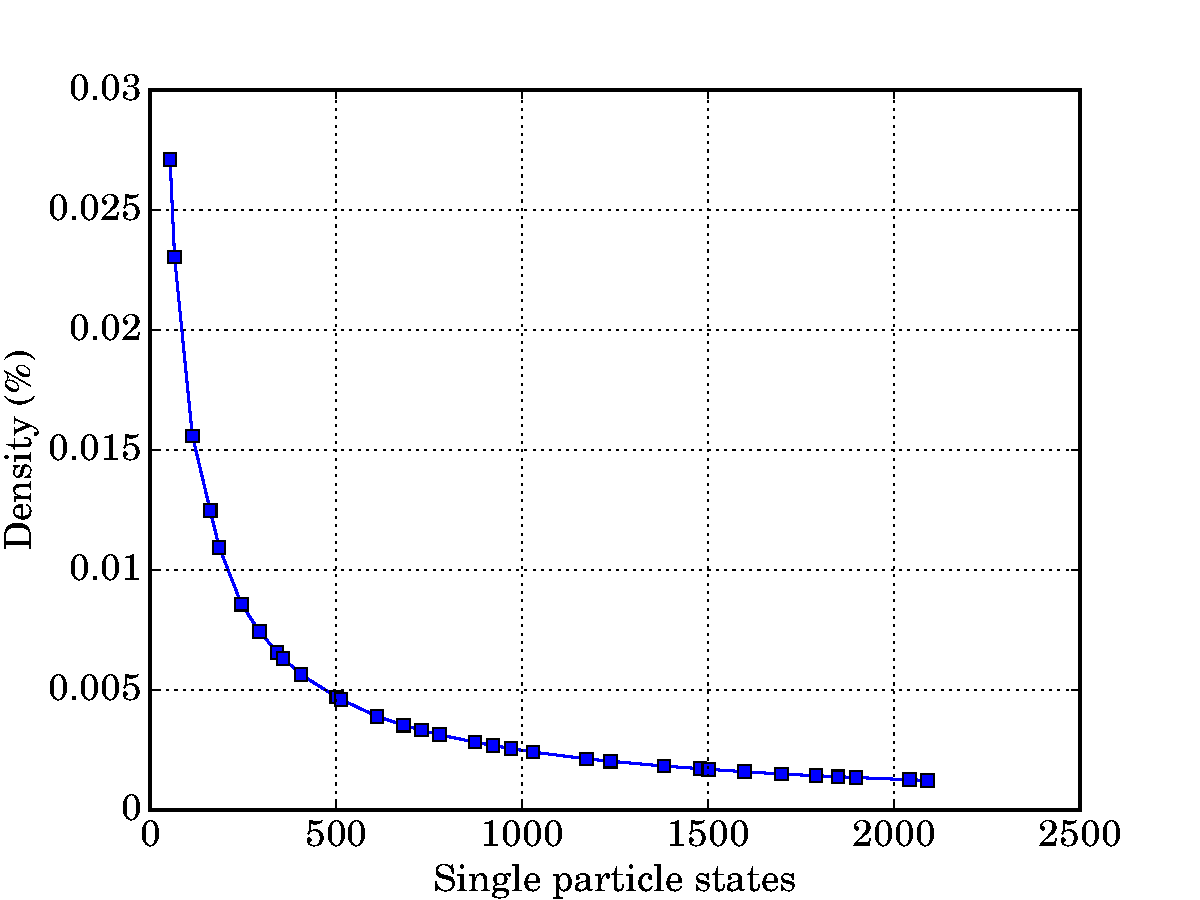
\includegraphics[width=0.5\textwidth]{Figures/T3_density.pdf}
		\caption{Density of the $T_3$ amplitudes for 14 particles, in the range of 3 to 40 shells, given in percentages.}
		\label{Implementation | fig | "T3 density"}
	\end{figure}
	
	At a simple level, there are two ways to store a matrix. The first is to simply store the whole thing as is, while the second is to only store the non-zero elements and their positions. In the first, we store $N\times M$ elements, where $N$ and $M$ are the matrix dimensions. In the second we store $3N'$ elements, where $N'$ is the number of non-zero elements, and the factor 3 arises due to having to store the matrix indices. Since we are working with such a \emph{sparse} matrix, the second approach sound quite appealing. Such an approach is called \emph{sparse matrix storage}.
	
	\subsection{Sparse matrix storage}
	When we say we have a sparse matrix, we mean it is a matrix of elements mostly equal zero. It is therefore better, memory wise, to store the matrix on the form
	
	\begin{equation*}
		\begin{pmatrix}
			\text{element value} \\ \text{row index} \\ \text{column index}
		\end{pmatrix}
	\end{equation*}
	
	Here we see that we would indeed have to store $3N'$ elements. A simple example is the matrix
	
	\begin{equation*}
		\begin{pmatrix}
			0 & 0 & 0 & 3.0 & 0 & 0 \\
			0 & 0 & 0 & 0 & 5.0 & 0 \\
			0 & 2.0 & 0 & 0 & 0 & 0 \\
			0 & 0 & 0 & 0 & 3.0 & 1.0 \\
			0 & 0 & 4.0 & 0 & 0 & 0 \\
		\end{pmatrix} \:,
	\end{equation*}
	
	\noindent which may be more efficiently stored sparsely,
	
	\begin{equation*}
		\begin{pmatrix}
			3.0 & 5.0 & 2.0 & 3.0 & 1.0 & 4.0 \\
			1 & 2 & 3 & 4 & 4 & 5 \\
			4 & 5 & 1 & 5 & 6 & 3 \\
		\end{pmatrix} \:,
	\end{equation*}
	
	\noindent since now we only store $3\times6$ numbers, as opposed to $5\times5$ numbers in the original case. The problem with this implementation, as reviewed in \cite{Hansen15}, is that it is far too slow when it comes to CC diagram calculations. The CC equations are solved by performing large summations, and in order to do it correctly, we need to find which elements of our sparse matrix to add. That means searching through the sparse amplitudes matrix looking for the two correct elements to multiply. By taking into account the number of non-zero elements we have to store, even with excellent search algorithms, such an approach quickly becomes too slow. Fortunately, summations may also be done as matrix products. However, the sparse matrix storage scheme is not suited for matrix inner products. This is where \emph{block matrix storage} is the best approach.
	
	\subsection{Block matrix storage}
	The block-implementation is actually more akin to the first method we mentioned of storing a matrix, but with a few more details in place. To better see how such an approach is used, we will now discuss matrix element storage for the interaction matrices, as they are more easily connected to conservation laws, which are important for the block-implementation. We know that our interaction matrix only has non-zero elements where momentum and spin conservation is upheld. That is,
	
	\begin{equation}
		\langle pk||rs\rangle = \delta_{\bm{k}_p + \bm{k}_q,\bm{k}_r + \bm{k}_s}\delta_{SS'} v_{pq}^{rs}\:.
	\end{equation}
	
	Therefore, we only have to store the parts of the interaction matrix where this applies. Unfortunately, the full interaction matrix does not divide nicely into "chunks" where momentum conservation applies. Instead, the conserving elements are spread throughout the matrix in a seemingly random manner. Therefore, we gather all elements with a certain spin and momentum conservation together in separate matrices, or \emph{blocks}. To imagine this, we may consider the interaction matrix of all particles\footnote{Remember that by "particle" we mean excitation above the Fermi level, just as we introduced in chapter \ref{MBQM | sec | "MBQM chapter"}.} to look as follows:
	
	\begin{equation}
		V_{pppp} = \left( V_{\bm{k}_{tot,1}}, V_{\bm{k}_{tot,2}}, V_{\bm{k}_{tot,3}}, \ldots, V_{\bm{k}_{tot,m}}\right)
	\end{equation}
	
	where $V_{tot,i}$ is a matrix made up of all pairs of states\footnote{By "pairs of states", we mean the rows and columns of $V_{tot,i}$ represent all states $|\alpha\beta\rangle$.} $(k_\alpha, k_\beta)$ that have total conservation $k_i = k_\alpha + k_\beta$. We call each total conservation ($k_i$) for a \emph{channel}. Our plan is then to only work in channels, and that two different channels will never "cross" to product non-zero values.\\
	
	Now we might start to wonder if this really helps or not, because what we gain in memory, we might loose in computation time. For example, the CC diagrams are contractions over states, not pairs of states, like $V_{tot,i}$ are indexed in. Does that mean we have to check every single row and columns in $V_{tot,i}$ to have the same indices as $T_{i}$ has? No, because, previously, we said a fair starting point for our amplitude iterations was to assume that the diagrams did not contribute to $t_{ij}^{ab}$, i.e starting with the MBPT2 approximation;
	
	\begin{equation}
		t_{ij}^{ab} = \frac{V_{ab}^{ij}}{f_i + f_j - f_a - f_b}
	\end{equation}
	
	This means our amplitude matrix, $T$, will have the same form as $V_{hhpp}$. If we then shape all interaction matrices ($V_{hhhh}$, $V_{hhpp}$, $V_{hphp}$, $V_{hhhp}$, $V_{ppph}$, and $V_{pppp}$) with the same order of indices, we may do matrix products without worries, meaning we now have a fully functioning approach to reduce memory usage \emph{and} we may use the basic linear algebra subprograms\footnote{These are highly efficient, standard routines for performing linear operations for vectors and matrices.} (BLAS \cite{blas}) to perform linear operations.
	
	\section{Block implementation}
	\label{Implementation | sec | "Block implementation"}
	The block implementation is easy to perform as long as we do not have to do in it different ways, which we, unfortunately, do. Before dealing with how to construct the block matrices, we need to make use of what is called a \emph{map}. A map, in the mathematical sense, can be considered to refer to any which way we could correlate two ways to format the same structure of elements. For example, the transpose of a matrix is simply an explicit way in which to take the elements of some matrix $A$ and put them into a matrix $A^T$, and is one example of a map, or mapping.\\
	
	This is quite relevant to mapping the elements of a tensor onto a two-dimensional matrix. Our map has to abide by certain restrictions in order to be useful. As mentioned, we want to be able to use the matrix inner-product function of the BLAS, which means matrix multiplication must be well-defined.\\
	
	Many of the diagrams in CCDT have problems when it comes to the block implementation, which is the cause for having to perform intermediate, demanding operations, as we soon shall see. We can start exploring the complications by means of some examples. The CCD $L_a$ diagram is quite simple. The sum goes as follows:
	
	\begin{equation}
		L_a \leftarrow \sum_{cd}\langle ab||cd\rangle t_{ij}^{cd} = v_{ab}^{cd}t_{ij}^{cd} \:,
	\end{equation}
	
	in which we decided to introduce the anti-symmetrized interaction matrix $v$, where the columns\footnote{Throughout this chapter, we use the convention that states in subscript are rows, while states in superscript are columns.} represent particle state pairs $(a,b)$ and the rows represent the particle state pairs $(c,d)$. We see that this translates easily into two dimensional matrices. As long as we now work in channels, we can perform this sum quickly and efficiently, which is good because the 4-particle interaction matrix is the largest sum to perform of the CCD diagrams.\\
	
	We know already that all CCD amplitudes not in $t_{ij}^{ab}$, when initialised, are zero, due to its declaration from MBPT2. Recalling how the concept of channels was introduced above, we also know that elements of different total momentum and spin do not overlap. For example, the elements of $(t_{ij}^{ab})_{k_{u_i}}$ do not contribute to $(t_{ij}^{ab})_{k_{u_j}}$, where $k_{u_i}\neq k_{u_j}$.\\
	
	However, consider the CCD $L_c$ diagram:
	
	\begin{equation}
	L_c \leftarrow \sum_{ck}\langle ak||cj\rangle t_{ik}^{cb} = v_{ak}^{cj}t_{ik}^{cb}
	\end{equation}
	
	Here it is not trivial to write the sum as matrix products, since we would multiply only over specific parts of the matrices, something the BLAS certainly will not do for us. Instead, we introduce the concept of \emph{alignment}.
	
	\subsection{Alignment}
	Aligning\footnote{The word "alignment" has been chosen to follow the convention of \cite{Hansen15}, who chose it since we align the matrix elements such that matrix products are possible.} the matrices means introducing new matrices where the columns and rows are aligned in such a way that we may do the sums as matrix products. Unfortunately, there are some complications with doing so. We decided to use the notation $\tilde{A}$ for the aligned version of a matrix $A$. This means that the matrices in $L_a$ are their own aligned version. The matrices in $L_c$ can be written as:
	
	\begin{equation}
		v_{ak}^{cj}t_{ik}^{cb} \quad\rightarrow\quad \tilde{v}_{aj}^{ck}\tilde{t}_{ib}^{ck} = \left(\tilde{v}\tilde{t}\right)_{aj}^{ib}
	\end{equation}
	
	This might seem simple, but it introduces new complications. Due to the declaration of $t_{ij}^{ab}$, we still require conservation of momentum and spin, i.e.
	
	\begin{equation}
		\bm{k}_i + \bm{k}_j = \bm{k}_a + \bm{k}_b \equiv \bm{K}
	\end{equation}
	
	However, the matrix product above is only non-zero for
	
	\begin{equation}
		\bm{k}_i + \bm{k}_k = \bm{k}_c + \bm{k}_b = \bm{k}_a + \bm{k}_k = \bm{k}_c + \bm{k}_j
		\label{Implementation | eq | mom. cons. for L_c}
	\end{equation}
	
	In order to work with both blocks and matrix contractions, we need to rewrite equation (\ref{Implementation | eq | mom. cons. for L_c}) such that the rows and columns of the matrices fulfil the conservation. That means we actually require the blocks to have conservation according to
	
	\begin{equation}
	\bm{k}_i - \bm{k}_b = \bm{k}_c - \bm{k}_k = \bm{k}_a - \bm{k}_j = \bm{k}_c - \bm{k}_k
	\label{Implementation | eq | mom. cons. for L_c, aligned}
	\end{equation}
	
	In other words, we let the rows hold particle-hole "states", while the columns hold hole-particle "states". Specifically, for the interaction matrix $v_{ak}^{cj}=\langle ak||cj\rangle$, the aligned rows give us the states $\langle a\cdot||\cdot j\rangle$, while the columns give us $\langle \cdot k||c\cdot\rangle$, where the dots just symbolise a lack of states. It is not too hard to imagine how we write this in code, but nonetheless we shall review the implementation in greater detail later on.\\
	
	We mentioned that we let the rows and columns represent pairs of states, which is not always true. For example, the diagram $Q_d$ has the form
	
	\begin{equation}
		t_{ik}^{cd}v_{kl}^{cd}t_{jl}^{ab} \quad\underset{\text{alignment}}{\longrightarrow}\quad \tilde{t}_{i}^{cdk}\tilde{v}_{l}^{cdk}\tilde{t}_{l}^{abj}\:,
	\end{equation}
	
	and we see that now the columns represent three states, and the rows represent one state. Of course, it does not matter one way or the other how many states are where; the principle behind alignment remains the same.\\
	
	Most of the doubles and triples diagrams require one alignment. The $T_{3b-e}$-diagrams require an additional realignment in-between matrix products, as there is no possible arrangement of indices for all three matrices that allows for a matrix contraction. This realignment can be problematic when it comes to parallelisation, but we shall discuss this point further later on. In table \ref{Implementation | table | "alignments"}, we show all alignments as they have been implemented. It is important to remember that, even though a matrix has been aligned, the elements still need to appear in the correct positions for the matrix product to be correct. This is where the use of \emph{dictionaries}, or \emph{maps}, is important.\\
	
	\begin{table}[h]
		\centering
		\captionsetup{width=.8\textwidth}
		\caption{The alignments, realignments (for $T_{3b-e}$), and product forms for the CCDT implementation. Symbols with $\tilde{a}$ are aligned, while those without are in their original form. Note that some diagrams require no ($L_a,\:L_b,\:Q_a$) or little ($T_{5f},\:T_{5g}$) alignment.}
		\begin{tabular}{ccccc}
			Diagram & Unaligned & Aligned & Realignment & Product \\ \hline
			$L_a$ & $v_{ab}^{cd}t_{ij}^{cd}$ & $v_{ab}^{cd}t_{ij}^{cd}$ & & $A_{ij}^{ab}$\\
			$L_b$ & $v_{kl}^{ij}t_{kl}^{ab}$ & $v_{kl}^{ij}t_{kl}^{ab}$ & & $A_{ij}^{ab}$\\
			$L_c$ & $v_{ak}^{cj}t_{ik}^{cb}$ & $\tilde{v}_{aj}^{ck}\tilde{t}_{ck}^{ib}$ & & $\tilde{A}_{ib}^{aj}$\\
			$Q_a$ & $t_{ij}^{cd}v_{kl}^{cd}t_{kl}^{ab}$ & $t_{ij}^{cd}v_{kl}^{cd}t_{kl}^{ab}$ & & $A_{ij}^{ab}$\\
			$Q_b$ & $t_{ik}^{ca}v_{kl}^{cd}t_{jl}^{db}$ & $\tilde{t}_{kc}^{ai}\tilde{v}_{kc}^{dl}\tilde{t}_{jb}^{dl}$ & & $\tilde{A}_{jb}^{ai}$\\
			$Q_c$ & $t_{kl}^{ca}v_{kl}^{cd}t_{ij}^{db}$ & $\tilde{t}_{klc}^{a}\tilde{v}_{klc}^{d}\tilde{t}_{ijb}^{d}$ & & $\tilde{A}_{ijb}^a$ \\
			$Q_d$ & $t_{ik}^{cd}v_{kl}^{cd}t_{jl}^{ab}$ & $\tilde{t}_{i}^{cdk}\tilde{v}_{l}^{cdk}\tilde{t}_{l}^{abj}$ & & $\tilde{A}_{i}^{abj}$ \\
			$D_{10b}$ & $v_{ak}^{cd}t_{ijk}^{cdb}$ & $\tilde{v}^{cdk}_{a}\tilde{t}_{ijb}^{cdk}$ & & $\tilde{A}_{ijb}^a$ \\
			$D_{10c}$ & $v_{kl}^{jc}t_{ikl}^{cab}$ & $\tilde{v}_{klc}^{j}\tilde{t}_{klc}^{abi}$ & & $\tilde{A}_{j}^{abi}$ \\
			$T_{1a}$ & $v_{bc}^{dk}t_{ij}^{ad}$ & $\tilde{v}_{bck}^{d}\tilde{t}_{ija}^{d}$ & & $\tilde{A}_{bck}^{ija}$ \\
			$T_{1b}$ & $v_{lc}^{jk}t_{il}^{ab}$ & $\tilde{v}_{l}^{jkc}\tilde{t}_{l}^{abi}$ & & $\tilde{A}_{jkc}^{abi}$ \\
			$T_{2c}$ & $v_{ab}^{de}t_{ijk}^{dec}$ & $\tilde{v}_{ab}^{de}\tilde{t}_{ijkc}^{de}$ & & $\tilde{A}_{ijkc}^{ab}$ \\
			$T_{2d}$ & $v_{ij}^{lm}t_{lmk}^{abc}$ & $\tilde{v}_{ij}^{lm}\tilde{t}_{lm}^{abck}$ & & $\tilde{A}_{ij}^{abck}$ \\
			$T_{2e}$ & $v_{id}^{al}t_{ljk}^{dbc}$ & $\tilde{v}_{ia}^{ld}\tilde{t}_{ld}^{bcjk}$ & & $\tilde{A}_{ia}^{bcjk}$ \\
			$T_{3b}$ & $t_{il}^{ad}v_{de}^{bl}t_{jk}^{ec}$ & $\left(\tilde{t}_{ld}^{ai}\tilde{v}_{eb}^{ld}\right)t_{jk}^{ec}$ & $(\tilde{t}\tilde{v})_{bai}^{e}\tilde{t}_{jkc}^{e}$ & $\tilde{A}_{jkc}^{bai}$ \\
			$T_{3c}$ & $t_{il}^{ad}v_{lm}^{jd}t_{mk}^{bc}$ & $\left(\tilde{t}_{ia}^{dl}\tilde{v}_{mj}^{dl}\right)t_{jk}^{ec}$ & $(\tilde{t}\tilde{v})_{ija}^{m}\tilde{t}_{m}^{bck}$ & $\tilde{A}_{ija}^{bck}$ \\
			$T_{3d}$ & $t_{il}^{ab}v_{de}^{cl}t_{jk}^{de}$ & $t_{il}^{ab}\left(\tilde{v}_{de}^{cl}\tilde{t}_{jk}^{de}\right)$ & $\tilde{t}_{l}^{abi}(\tilde{v}\tilde{t})_{jkc}^{l}$ & $\tilde{A}_{jkc}^{abi}$ \\
			$T_{3e}$ & $t_{ij}^{ad}v_{lm}^{kd}t_{lm}^{bc}$ & $\left(\tilde{t}_{ija}^{d}\tilde{v}_{lmk}^{d}\right)t_{lm}^{bc}$ & $(\tilde{t}\tilde{v})_{ijka}^{lm}\tilde{t}_{lm}^{bc}$ & $\tilde{A}_{ijka}^{bc}$ \\
			$T_{5a}$ & $t_{il}^{ad}v_{lm}^{de}t_{mjk}^{ebc}$ & $\tilde{t}_{ia}^{dl}\tilde{v}_{me}^{dl}\tilde{t}_{me}^{bcjk}$ & & $\tilde{A}_{ia}^{bcjk}$ \\
			$T_{5b}$ & $t_{li}^{de}v_{lm}^{de}t_{mjk}^{abc}$ & $\tilde{t}_{i}^{del}\tilde{v}_{m}^{del}\tilde{t}_{m}^{abcjk}$ & & $\tilde{A}_{i}^{abcjk}$ \\
			$T_{5c}$ & $t_{lm}^{da}v_{lm}^{de}t_{ijk}^{ebc}$ & $\tilde{t}_{lmd}^{a}\tilde{v}_{lmd}^{e}\tilde{t}_{ijkbc}^{e}$ & & $\tilde{A}_{ijkbc}^{a}$ \\
			$T_{5d}$ & $t_{ij}^{ad}v_{lm}^{de}t_{lmk}^{bec}$ & $\tilde{t}_{ija}^{d}\tilde{v}_{lme}^{d}\tilde{t}_{lme}^{bck}$ & & $\tilde{A}_{ija}^{bck}$ \\
			$T_{5e}$ & $t_{il}^{ab}v_{lm}^{de}t_{jmk}^{dec}$ & $\tilde{t}_{l}^{abi}\tilde{v}_{l}^{dem}\tilde{t}_{jkc}^{dem}$ & & $\tilde{A}_{jkc}^{abi}$ \\
			$T_{5f}$ & $t_{ij}^{de}v_{lm}^{de}t_{lmk}^{abc}$ & $t_{ij}^{de}v_{lm}^{de}\tilde{t}_{lm}^{abck}$ & & $\tilde{A}_{ij}^{abck}$ \\
			$T_{5g}$ & $t_{lm}^{ab}v_{lm}^{de}t_{ijk}^{dec}$ & $t_{lm}^{ab}v_{lm}^{de}\tilde{t}_{ijkc}^{de}$ & & $\tilde{A}_{ab}^{ijkc}$
		\end{tabular}
		\label{Implementation | table | "alignments"}
	\end{table}
	
	A dictionary is a object used in computing that, given some \emph{key}, returns a value. That is, we can make a dictionary $D$ that looks as
	
	\begin{center}
	\begin{tabular}{cc}
		key & value \\
		car & 12 \\
		candlestick & -17 \\
		frumblesnuff & 34
	\end{tabular}
	\end{center}
	
	Now, if we call $D(\text{candlestick})$, we get back the value $-17$. Of course, the keys can be whatever we desire, like string, integers, floats, etc, and the same goes for the values. In our case, the keys will be unique identifiers for a set of states. For example, the $T_2$ amplitudes can be gotten for a set of states $i$, $j$, $a$, and $b$ by some unique identifier, 
	
	\begin{equation}
		Id(i,j,a,b) = a + bN_p + iN_p^2 + jN_p^2N_h\:,
	\end{equation}
	
	which will serve as integer keys. Obviously the amplitudes themselves will be floats, so the values of the map will be floats. This extends easily to all the other matrices as well. In C++, we use the standard library maps, which has the exact same functionality as dictionaries.\\
	
	Consider a dictionary $D$, that takes 6 arguments, $\{i,\:j,\:k,\:a,\:b,\:c\}$, and returns an index, which, when used together with an array that holds the $T_3$ amplitudes, gives us element $t_{ijk}^{abc}$. If we let $A$ be the array of amplitudes, then
	
	\begin{align}
	D(i,j,k,a,b,c) &= I \\
	A(I) = t_{ijk}^{abc}
	\label{Implementation | eq | "T3 element retrieval"}
	\end{align}
	
	Our matrices are constructed with the use of index matrices, such as those we explained previously. For example, the unaligned matrix $t_{ijk}^{abc}$ would have rows where each row is some selection $\{ijk\}$, where\footnote{Later on, when we start discussing index matrices, we shall be using phrases such as \texttt{ppmm\_hhpp} to signify which how we have done shift of unique identifiers. The notation means plus-plus-minus-minus for hole-hole-particle-particle, i.e. $+k_u(h1)+k_u(h2)-k_u(p1)-k_u(p2)$.}
	
	\begin{equation}
	k_i+k_j+k_k = k_u
	\end{equation}
	
	The columns would be the same, such that each column is some selection $\{abc\}$ where
	
	\begin{equation}
	k_a+k_b+k_c = k_u
	\end{equation}
	
	In order to insert the correct amplitude for a row and column, we have to find it in the amplitude array $A$. From the column and row, we can figure out which indices we have (due to the index matrices predefined), and insert them into the dictionary $D$, just like we described above. If we do this for the whole matrix, we will have constructed channel $k_u$ for the $T_3$ matrix.\\
	
	It should be apparent that this approach does not change with alignment. If we instead want to make a matrix in the shape of $t_{ij}^{abck}$, then while we will be working with another set of channels and index matrices, the approach is the same. However, since the CC diagrams contain no apparent repeated manner in which the index summations are done, it is difficult to make a general alignment function that places the amplitudes correctly in matrices for all diagrams. This is why, for our implementation, each diagram has its own matrix construction function. A golden rule when it comes to code writing is to never write repeated code, as the possibility of error increases with each line, but we found no way of avoiding it.\\
	
	This approach is the one used throughout our implementation. Although we will discuss the downsides of the use of dictionaries later on, we note that making a matrix from an array \emph{must} use some sort of search function, whether it is done through the std library, some other library, or our own search function, perhaps even in parallel. Such a search function will use time, and the most speedup to be gained in any implementation like this is by optimising the search function.
	
	\subsection{Permutations}
	\label{Implementation | sec | "permutations"}
	Most of the CC diagrams have permutations of indices. In the CCD diagrams, the possible permutations are $\hat{P}_{ij}$, $\hat{P}_{ab}$, and $\hat{P}_{ij}\hat{P}_{ab}$. This is not very many possible permutations, and they are quite simple to perform. That is, if we stored the terms from a diagram sum in a dictionary, we could perform a permutation by simply calling different elements of the sum. Assume we are calculating a diagram in some form
	
	\begin{equation}
		t_{ij}^{ab} \leftarrow \hat{P}D_{ij}^{ab}\:,
	\end{equation}
	
	where $D_{ij}^{ab}$ is the outcome of the summation of internal indices, and we have stored if as a map, say $M_D$, using the same identity function to generate keys as the one we use for the $T_2$ amplitude map. If now $\hat{P} = \hat{P}_{ab} = 1-P_{ab}$, then the permutation is simply
	
	\begin{equation}
		t_{ij}^{ab} \leftarrow \left[D_{ij}^{ab} - D_{ij}^{ba}\right] \:,
	\end{equation}
	
	where we find the two elements $D_{ij}^{ab}$, $D_{ij}^{ba}$ by
	
	\begin{align}
		\begin{split}
		D_{ij}^{ab} &= M_D\left(\text{id}(i,j,a,b)\right) \\
		D_{ij}^{ba} &= M_D\left(\text{id}(i,j,b,a)\right)
		\end{split}
	\end{align}
	
	We have not bothered with a more optimised scheme with which to do the CCD permutations, since, as we have mentioned at the start of this chapter, the $T_2$ amplitudes are few in comparison to the $T_3$ amplitudes. This means that the $T_2$ diagram maps are much smaller and take much less time to search through, than the $T_3$ diagram maps. In CCDT, however, there are up to 4 permutation operators on a single diagrams. Take, for example, the diagram $T_{1a}$:
	
	\begin{align}
		\begin{split}
		T_{1a} :&= \hat{P}(a/bc)\hat{P}(k/ij)\sum_d \langle bc|| dk\rangle t_{ij}^{ad} \\
		& = (1-\hat{P}_{ab} - \hat{P}_{ac})(1-\hat{P}_{ki}-\hat{P}_{kj})D_{ijk}^{abc} \\
		&= \big[1-\hat{P}_{ab}-\hat{P}_{ac}-\hat{P}_{ki}-\hat{P}_{kj} \\
		&\quad\quad\: + \hat{P}_{ab}\hat{P}_{ki} + \hat{P}_{ab}\hat{P}_{kj} + \hat{P}_{ac}\hat{P}_{ki} + \hat{P}_{ac}\hat{P}_{kj} \big]D_{ijk}^{abc}
		\end{split}
	\end{align}
	
	where $D_{ijk}^{abc}$ is the sum for some diagram. If we were still to use dictionaries to perform permutations, we would have to do as many search calls as there are terms in the equation above. As stated, we would like to minimise search calls as much as possible, so an alternate approach is better. In the process of writing, we attempted two different approaches, mostly out of necessity.\\
	
	The first approach consisted of storing the permutations beforehand. This is very memory intensive for aligned matrices\footnote{We would have to store all the permutations, for each diagram.}. Fortunately, if we use re-alignment of diagrams, i.e. write $\tilde{D}_{ija}^{cbk}$ as $D_{ijk}^{abc}$, we can simply store the permutations of columns and rows, since there will never be a permutation between hole- and particle-indices. Therefore, to do permutations on the amplitude contribution $\tilde{D}$, we use the dictionary to set all the elements of $\tilde{D}$ into a temporary, empty array\footnote{By empty, we mean all components are zero.} $A'$ in same layout as for the amplitude array $A$, meaning the element number $i$ in $A'$ has the same state indices as element $i$ in $A$. We then construct the direct channels $D$ using this temporary array. We have then effectively done a remapping
	
	\begin{equation}
		\tilde{D}_{ija}^{cbk} \:\rightarrow\: D_{ijk}^{abc}
	\end{equation}
	
	By now swapping the rows and columns of $D$, using some object telling us, for example, which rows go where if we interchange $i\leftrightarrow k$. To be specific, we can consider how to do this permutation, meaning we want to find $\hat{P}(ik)t_{ijk}^{abc} = t_{ijk}^{abc} - t_{kji}^{abc}$. Now, due to our whole channel regime, we cannot just change the indices in some 4- or 6-dimensional tensor. Instead, we need to interchange columns and rows in matrices, such if that two rows, $(i,j,k)$ and $(l,m,n)$, that become permuted as
	
	\begin{align}
	(i,j,k) \quad&\overset{\hat{P}}{\longrightarrow}\quad (i',j',k') \\
	(l,m,n) \quad&\overset{\hat{P}}{\longrightarrow}\quad (l',m',n')
	\end{align}
	
	and fulfil
	
	\begin{align}
	(i,j,k) &= (l',m',n') \\
	(l,m,n) &= (i',j',k') \:,
	\end{align}
	
	then we switch the two rows $(i,j,k)$ and $(l,m,n)$. In matrix form, such a permutation can, for example, be seen as
	
	\begin{equation*}
	\begin{matrix}[cccc|cccccc]
	&   &   & a & 10 & 9  & 15 & 11 & 17 & 14\\
	&   &   & b & 11 & 14 & 14 & 18 & 23 & 15\\
	&   &   & c & 16 & 17 & 13 & 20 & 20 & 23\\
	i & j & k &   &    &    &    &    &    &   \\ \hline
	0 & 1 & 2 & & a_{11} & a_{12} & a_{13} & a_{14} & a_{15} & a_{16}\\
	0 & 2 & 1 & & a_{21} & a_{22} & a_{23} & a_{24} & a_{25} & a_{26}\\
	1 & 0 & 2 & & a_{31} & a_{32} & a_{33} & a_{34} & a_{35} & a_{36}\\
	1 & 2 & 0 & & a_{41} & a_{42} & a_{43} & a_{44} & a_{45} & a_{46}\\
	2 & 0 & 1 & & a_{51} & a_{52} & a_{53} & a_{54} & a_{55} & a_{56}\\
	2 & 1 & 0 & & a_{61} & a_{62} & a_{63} & a_{64} & a_{65} & a_{66}\\
	\end{matrix}
	\quad\overset{\hat{P}(ik)}{\longrightarrow}\quad
	\begin{matrix}[cccc|cccccc]
	&   &   & a & 10 & 9  & 15 & 11 & 17 & 14\\
	&   &   & b & 11 & 14 & 14 & 18 & 23 & 15\\
	&   &   & c & 16 & 17 & 13 & 20 & 20 & 23\\
	k & j & i &   &    &    &    &    &    &   \\ \hline
	2 & 1 & 0 & & a_{61} & a_{62} & a_{63} & a_{64} & a_{65} & a_{66}\\
	1 & 2 & 0 & & a_{41} & a_{42} & a_{43} & a_{44} & a_{45} & a_{46}\\
	2 & 0 & 1 & & a_{51} & a_{52} & a_{53} & a_{54} & a_{55} & a_{56}\\
	0 & 2 & 1 & & a_{21} & a_{22} & a_{23} & a_{24} & a_{25} & a_{26}\\
	1 & 0 & 2 & & a_{31} & a_{32} & a_{33} & a_{34} & a_{35} & a_{36}\\
	0 & 1 & 2 & & a_{11} & a_{12} & a_{13} & a_{14} & a_{15} & a_{16}
	\end{matrix}
	\end{equation*}
	
	By adding these matrices, we will have calculated $\hat{P}(ik)t_{ijk}^{abc}$.\\
	
	The second approach consisted of assuming that every element in the diagram sums were some permutation for another element. To explicate, assume we have some diagram element $D_{ijk}^{abc}$. We know that, without permutation, this element contributes directly to the same amplitude, i.e.
	
	\begin{equation}
		t_{ijk}^{abc} \leftarrow D_{ijk}^{abc}
	\end{equation}
	
	However, we know\footnote{To realise this, go back to the way in which we do the $T_2$ permutations, and consider to what the map actually returns when we swap two indices.} that this element is also a $i\leftrightarrow j$ permutation of the element $D_{i'j'k'}^{a'b'c'}$, where
	
	\begin{align}
	\begin{split}
	i &= j' \\
	j &= i' \\
	k &= k'
	\end{split}
	\end{align}
	
	In other words, we may use
	
	\begin{align}
		\begin{split}
		t_{i'j'k'}^{a'b'c'} &= \hat{P}(ik)D_{i'j'k'}^{a'b'c'} \\
		&= D_{i'j'k'}^{a'b'c'} - D_{ijk}^{abc}
		\end{split}
	\end{align}
	
	At first, this might seem utterly pointless, since we would have to search through all the $D$ elements to find $D_{ijk}^{abc}$, when working with $D_{i'j'k'}^{a'b'c'}$. However, knowing that this specific diagram has a permutation of $i$ and $j$, we can, when going through all the elements of $D$, simply let each element $D_{ijk}^{abc}$ contribute to both\footnote{It is important to be mindful of signs when doing this. Each swap of indices gives a minus sign.} $t_{ijk}^{abc}$ and $t_{jik}^{abc}$. Mathematically, this approach is show by
	
	\begin{align}
		\begin{split}
			t_{ijk}^{abc} &\leftarrow \hat{P}(ik) D_{ijk}^{abc} \\
			\underset{\hat{P}(ik)\big|}{\longrightarrow}\quad \hat{P}(ik)t_{ijk}^{abc} &\leftarrow \hat{P}^2(ik)D_{ijk}^{abc} = D_{ijk}^{abc}
		\end{split}
	\end{align}
	
	The latter approach is nice in the sense that we need not do any sort of remapping, but it is at the cost of having to do another map search per permutation operator, per diagram element. However, it is problematic when it comes to parallellisation. Since we, ultimately, would like to work on channels in parallel, the second approach means we might try to write to the same element from several processes. We will discuss parallellisation in more depth below.
	
	\section{Parallelisation}
	Parallelisation is a necessity for CCDT, even for the most efficient implementations, simply due to the immense increase in computational time and memory requirements when we move up in system size. There are two options for C++ when it comes to parallelisation, one being use of MP (multi-processing) and the other being MPI (multi-processing interface). We have attempted both options as a means of speedup, but found complications in both cases, which severely limited the use of parallel computation.\\
	
	We briefly remind the reader that MP makes use of \emph{threads}, which means several processors do a series of operations at the same time, but use a shared memory. We call this \emph{multi-threading}. When using MP, any object that is read from memory inside the for-loop \emph{will not} be copied for each thread. This approach was, at first, thought difficult as the dictionaries used were not thought thread-safe. However, this was solved when we found that dictionaries in the standard C++ libraries (\texttt{std::unordered\_map}) have two functions for retrieving elements, one of which is thread safe and the other is not. Therefore, OpenMP is used as a means of searching the dictionaries for elements, giving significant speedup.\\
	
	Due to the misconception regarding thread-safe dictionaries, we considered MPI a more promising parallel environment, initially. Using MPI, by letting each process have a copy of the same index dictionary, each process could be given a subsection of channels to handle. This means each process would calculate the contributions from $n$ of $m$ channels, and afterwards return an array with the new amplitudes. To then do the permutations by shifting columns and rows, we let only one world perform permutations, as this was easy to use together with OpenMP. Unfortunately, such an approach suffers from a massive increase in memory requirements, since we require a copy of the amplitude arrays and dictionaries for each world, as well as a copy if the index matrices. An improved implementation could perhaps avoid the difficulties by letting each world only hold part of the full system objects. Such an implementation would perhaps suffer from increased communication time.\\
	
	\section{Practical aspects and possible pitfalls}
	Should there ever be any future studies similar to to our own, we shall here list every important practical issue when it comes to a CC implementation like ours. We have mostly concerned ourselves with the triples part of the implementation, as a CCD program is not nearly as demanding for the system sizes used here. We shall also explain which pitfalls to beware, as some of them are subtle and can take much time to find and fix. 
	
	\begin{comment}
	\subsection{Matrix construction; memory versus computational efficiency}
	Since there are so many CC amplitudes we have to store, especially in the CCDT scenario, we store only the non-zero values. However, due to the need for alignment of products in diagram contributions, if we stored all the elements as matrices, we would be storing the same amplitude many times. This brings about an enormous increase in memory use, simply for storing the same element again and again but in different matrices. This is why we discussed the use of dictionaries\\
	
	Since the most efficient way to store the amplitudes is to store each amplitude only once, we can hold them all in an array. We then construct the aligned matrices "on the go", i.e. for each channel we construct the matrices, multiply them, and map the product back into array form.\\
	
	There are several ways to go about such an "on-the-go" construction. The most memory efficient approach is to let our array be a dictionary\footnote{A dictionary is an object that connects keys to values.}, where the key is an integer made uniquely for the quantum numbers, such as the index function
	
	\begin{equation}
		Id(i,j,k,a,b,c) = a + bN_p + cN_p^2 + iN_p^2 + jN_p^2N_h + kN_p^2N_h
	\end{equation}
	
	and the value is the amplitude corresponding to the identity, i.e. $t_{ijk}^{abc}$. As is the rule rather than the exception when it comes to optimisation, such a memory efficient approach uses too much time. A dictionary uses a search algorithm, and even when using very efficient dictionaries, we will not escape the fact that searching for elements takes time.\\
	
	Another approach is keep the matrices for each channel, but rather than let them hold the amplitudes themselves, they hold indices to the array which holds the amplitudes. This is a bit of an in-between approach to optimization. Since finding array elements by indexing uses no search algorithm\footnote{The array, given an index, points us directly to the location of the value in the computer memory, which is about as fast as it gets.}, we sacrifice some memory (storing all the matrices with indices) to gain computational efficiency (avoiding search algorithms). Now, rather than storing the same amplitude again and again in different matrices, we store the same index again and again. Since the function $Id$ returns an integer, we will be storing integers rather than float-point numbers just as the amplitude itself is stored. For a sufficiently large basis size, integers of type signed int in c++ standard will reach maximum size. That is, it "runs out of numbers". We found it necessary to instead use unsigned 64-bit integers instead. Fortunately, many of the CC diagrams have the same channels, so we need only store a channel once, and let all diagrams use that same channel. This is a small, but important, point.\\
	
	For this work, we decided to combine the two approaches, to store matrices with indices for the direct $t_{ijk}^{abc}$ channel, as it is used frequently together with diagram permutations, and to use maps to make all alignments. This means we will sacrifice some CPU time on searching through maps, to gain a lot of memory that would otherwise be wasted on storing matrix alignments used only for single diagrams. It also means we will sacrifice some memory on storing the direct channel, to gain a lot of CPU time due to our repeated shuffling of rows and columns in order to do permutations.
	\end{comment}
	
	\subsection{Alignment and re-alignment; careful indexing}
	When implementing channels and alignment of matrices, we need to be careful with the construction and deconstruction of matrices. While we would like a general matrix construction function, making one becomes tricky because an aligned matrix only gives correct results if it is made with care in respect to the other matrix with which a product will be made. To be more specific, consider the diagram $T_{1a}$ again:
	
	\begin{equation}
		T_{1a} := \hat{P}(a/bc)\hat{P}(k/ji)\sum_d \langle bc|| dk\rangle t_{ij}^{ad}
	\end{equation}
	
	Writing the sum in matrix form, and dropping the permutations, we get:
	
	\begin{equation*}
		v_{bc}^{dk}t_{ij}^{ad} \:\rightarrow\: t_{ijk}^{abc}
	\end{equation*}
	
	We decide to give this element a unique identifier, given by the function
	
	\begin{equation*}
		Id(i,j,k,a,b,c) \:,
	\end{equation*}
	
	Now, to sum over the index $d$ by using matrix multiplication, we write the product in aligned form:
	
	\begin{equation*}
		\tilde{v}_{bck}^{d}\tilde{t}_{d}^{ija} \:\rightarrow\: \tilde{t}_{bck}^{ija}
	\end{equation*}
	
	Comparing the unaligned and aligned expressions, we see that we would have to use the index function differently when realigning. That is to say, both expressions contribute to the amplitude $t_{ijk}^{abc}$, 
	but for the matrix $t_{bck}^{ija}$, we have to careful. Since we are working with matrices that hold these indices, they have a specific structure, made by the program itself. Therefore, the rows are given by a list where each element is an array $(b,c,k)$, while for the columns we have $(i,j,a)$. Therefore, to use the index function, we have to send row or columns indices in different orders, depending on which alignment we are realigning. To clarify, let us write column arrays as $\bm{C} = (b,c,k)$ and row arrays as $\bm{R} = (i,j,a)$. To get the correct element, we would have to call the identity function as
	
	\begin{equation*}
		Id(\bm{R}_1, \bm{R}_2, \bm{C}_3, \bm{R}_3, \bm{C}_1, \bm{C}_2)
	\end{equation*}
	
	Similar logic is necessary for all alignment and re-alignment cases.
	
	\begin{comment}
	\subsection{Parallel implementation; thread-safe array access}
	Obviously, parallel computing is a must for program speedup. The implementation of choice mentioned in the previous section hits a snag when it comes to parallellisation of matrix construction. To "fill up" the matrices with amplitudes faster, we wish to do so in parallel, letting each process fill a part of the matrix. However, even when accessing different parts of the same array, simultaneous access to an array from several processes gives memory issues. In other words, the array access is not \emph{thread-safe}.
	\end{comment}
	
	\subsection{Aspects of optimisation}
	\label{Implementation | sec | "optimisations"}
	When a program's requirements outgrow the capabilities of a computer, we can either get a better computer\footnote{In our case, this would be the supercomputer Abel}, or we can make the code more efficient. In order words, we wish to optimise it. For this work, several different attempts at optimisations were performed, but not all paid off. Here, we list both optimisations that turned out to be a waste of time due to any number of complications, and those that were quite gainful, such that any future work may avoid such time drains.\\
	
	\begin{itemize}
		\item Using MPI: We attempted to use MPI as a means of calculating the channel contributions for each diagram in parallel. However, letting each MPI world hold all the objects present in the serial code means multiplying the memory usage by how many MPI worlds we are running. Since much of the problem with solving the CC equations is to do with memory demands, this is hardly a promising way to do it.
		
		Other, more efficient ways to use MPI are, of course, possible. One is by letting each world hold only part of the $T_3$ dictionary and the amplitude array elements of which that part of the dictionary has mapped. We would then have to construct a matrix by adding together partly filled matrices from each MPI world. This approach uses much communication, and therefore has much overhead.
		
		\item The use of the index matrix structure pays off only when the number of rows and columns are nearly equal. In the case of the $T_{5b}$ and $T_{5c}$ diagrams, we require the index matrix for single indices and those for 5 indices. However, the single-index matrix will only have one column per channel. This means that all the matrices in $T_{5b}$ and $T_{5c}$ will have $N_c\times 1$ matrices\footnote{Where $c$ signifies that $N$ would change with channels.}. This means we would be storing $5N_c+1$ integers to find $5N_c$ amplitudes. This is pointless, and we might as well store the amplitude array indices in matrix form. We already know that storing indices directly in matrices is much faster than performing index searches, and this implementation was no different. Additionally, we no longer had to keep the largest of the index matrices, thus freeing up a bit of memory.
		
		\item When it comes to the topic of maps in computer language, the choice of map is important. For example, if we knew that we had to go through keys in a certain order every time, we would use the normal \texttt{std::map} of the C++ standard library. If we require random access, we could use the \texttt{std::unordered\_map}, which is a hashmap. In our case, we settled on a modified variant of the \texttt{std::unordered\_map}, called \texttt{sparsepp} \cite{sparsepp}. We show a simple time profiling of the three map types in figure \ref{Results | table | CCDT time table}.
		
		\begin{figure}[h]
			\centering
			\captionsetup{width=.8\textwidth}
			\begin{tabular}{ll}
				Implementation & Time (s) \\%(new implementation, be careful, took 512s) (made fix, now -0.4639628744093380, took 1004s) (made another fix, also -0.4639628744093380, but took 206s)
				one std map & 1004 \\
				one spp sparse\_hash\_map for each thread & 512 \\
				one spp sparse\_hash\_map & 206
			\end{tabular}
			\caption{CCDT time consumption for HEG with different implementations, for $N_s=114$, $N_h=14$, $r_s=1.0$, and $10^{-16}$ precision. All examples were run with 4 threads in OpenMP.}
			\label{Results | table | CCDT time table}
		\end{figure}
	\end{itemize}
	
	\subsection{Omitted, possible optimisations}
	There are several tweaks to the implementation presented here that might provide more efficient code when it comes to a parallel running environment with regards to both memory and runtime. The most significant are presented here. When it comes to the doubles diagrams, the $T_2$ dictionaries that are searched for matrix construction are so small in comparison to the $T_3$ dictionaries, that any focus on optimised $T_2$ search does very little for the overall runtime. Therefore, only the $T_3$ dictionary search has been considered for optimisation.
	
	\begin{itemize}
		\item The use of index matrices in our implementation means having one index matrix for each necessary alignment. That is, we store 21 different index matrices, the most demanding of which are, by far, the \texttt{pppm\_ppph}, \texttt{pppmm\_hhhpp}, and \texttt{pppmm\_ppphh} index matrix. Since it was difficult to know, at the time we were writing the code, just how demanding these objects become, they caused many problems as we managed to run larger and larger systems sizes. After having written them as efficiently as we could, we still found they needed much CPU time and memory\footnote{Far more memory than storing the $T_3$ amplitudes themselves.}. Of course, when calculating them takes so much time, we realised that calculating and storing them at the start of the program was a necessity. If we chose to calculate the channels repeatedly for each diagram and CC iteration, the computation time would increase to ludicrous lengths.\\
		
		However, if a scheme where storing only a few index matrices were possible, it would offer extremely efficient memory use. If there was a way to store, for example, only a \texttt{ppp\_hhh} and \texttt{ppp\_ppp} index matrix, it would use about 0.3 Gb\footnote{That is, using 16-bit numbers to store states. Unsigned 16-bit integers can take numbers up to  65536 in base 10. Since we are working with, at the most, 2282 states, 16-bit is actually far bigger than we need. We would use fewer bits if we could, but unfortunately, 8-bit integers can only take up to 256 numbers, which is too little.} for 66 particles and 1030 states. To only use two such matrices, we would have to store vectors pointing to which elements of the two matrices to combine in order to get, for example, \texttt{pppmm\_hhhpp}. This means going through both \texttt{ppp\_hhh} and \texttt{ppp\_ppp}, calculating channels for the combined arrays, and storing them in other arrays (for example replacing our current \texttt{indexHolders}). Of course, these new \texttt{indexHolders} would require much more memory, but we believe not greater than our current index matrix. If we had more time, we would have looked into this approach as it seems the most likely to provide optimisation to both CPU time and memory consumption.
		
		\item While our implementation is fully parallel when it comes to block matrix construction and matrix multiplication, it leaves much to be desired when destructing the matrix products, as mentioned in our section on parallelisation. Although we have been unable to think of a means to prevent having to use OpenMP communication when writing to the new $T_3$ amplitudes, we have no reason to believe it is not possible.
	\end{itemize}
	
	\begin{comment}
	\subsection{Index matrix contiguous memory}
	The final pitfall we should mention is a subtle one. Matrices can, as we mentioned in our discussion of the sparse and block approaches, be either sparse or dense\footnote{We have not mentioned dense matrices before now. A dense matrix is a matrix that is, well, dense. There are many non-zero values, as opposed to sparse matrices.}. If they are sparse, then we store the elements and their positions, just as discussed earlier. Dense matrices are stored contiguously in the computer memory. That way, the computer does not know the exact position of each element, but rather where the matrix starts and ends. Calling a specific matrix elements makes the computer start at the matrix beginning, and work it's way to the element in question. This makes dense matrix storage very efficient, both with regards to memory and speed. However, note well that it requires a contiguous section in the computer memory.\\
	
	Every element in our \texttt{blockArray}-matrices are of use, and the matrices are therefore not sparse at all. Consequently, it is very advantageous to use dense matrices. Unfortunately, the larger index matrices, for $ppph$, $hhhpp$, and $ppphh$, quickly become \emph{enormous} when increasing the system size. This was not a problem we encountered until running CCDT for 38 particles and 1300 single particle states. While the problem can be easily circumvented by splitting up the matrices into several matrices, thereby not requiring quite as big, contiguous memory chunks, there was no time left to implement such a rewrite of our implementation.
	\end{comment}
	
	\section{Program structure and hierarchy}
	Here we outline the structure of the program used for the calculations herein. We assume the reader to be acquainted with typical programming concepts such as \emph{classes}, \emph{object-oriented programming}, and \emph{pointers/references}. In section \ref{Implementation | sec | "example"}, we shall give a detailed example, with code sections, of the $T_{5a}$ diagram and all the steps involved in it's calculation. Naturally, we will assume basic knowledge in C++ conventions for this example, but otherwise we shall speak in terms of pseudo-code.
	
	\subsection{Classes}
	There are 5 classes used here for performing the CC method, one of which is the usual "main" class, and an additional class containing the model details, such as the HEG or the Minnesota potential. They are
	
	\begin{itemize}
		\item \texttt{Master}
		\item \texttt{MakeIntMat}
		\item \texttt{MakeAmpMat}
		\item \texttt{Diagrams}
		\item \texttt{System}
		\begin{itemize}
			\item \texttt{HEG}
			\item \texttt{MP}
			\item \texttt{CHIRAL}
		\end{itemize}
	\end{itemize}
	
	\subsection{System class}
	The system class holds all the specific details of the state space and Hamiltonian for the system in mind. The currently implemented models are the HEG, the Minnesota potential for neutron matter, and the Chiral potential.\\
	
	The class has multiple functions that are used throughout the other classes:
	
	\begin{itemize}
		\item \texttt{makeStateSpace}: Calculates all possible states, meaning quantum number combinations, up to the desired closed shell. We store the states in a matrix such that each column possesses the quantum numbers belonging to a state. Algorithm \ref{Implementation | algo | "makestatespace"} shows the structure.
		
		\begin{algorithm}[H]
			$i=0$\;
			\For{$n^2 \:\in\: [0,N_b]$}{
				\For{$n_x \:\in\: [-n^2,n^2]$}{
					\For{$n_y \:\in\: [-n^2,n^2]$}{
						\For{$n_z \:\in\: [-n^2,n^2]$}{
							States.col(i+0) = $(n^2,n_x,n_y,n_z,S_z=+1,T_z=+1)$\;
							States.col(i+1) = $(n^2,n_x,n_y,n_z,S_z=-1,T_z=+1)$\;
							States.col(i+2) = $(n^2,n_x,n_y,n_z,S_z=+1,T_z=-1)$\;
							States.col(i+3) = $(n^2,n_x,n_y,n_z,S_z=-1,T_z=-1)$\;
							$i = i+4$\;
						}
					}
				}
			}
			\BlankLine
			\BlankLine
		\caption{The \texttt{makeStateSpace} function}
		\label{Implementation | algo | "makestatespace"}
		\end{algorithm}
		\BlankLine
		\BlankLine
		Note here that we have included isospin as quantum numbers. We found a study of symmetric matter to be far too demanding, as we then have to store \emph{all} amplitudes and interactions, as opposed to those with the requirement $i<j<k$ and $a<b<c$. Therefore, we have chosen to stick to systems with identical particles, either neutrons or electrons, depending on system.
		
		\item \texttt{assym}: The anti-symmetric inner product $\langle pq||rs\rangle$ for four arguments $\{p,q,r,s\}$. These functions have analytic expressions which we have given in equation (\ref{Int.Nucl.Mat | eq | "Minnesota potential"}) for the Minnesota potential and equation (\ref{MBQM | eq | "Ewald energy"}) for the HEG.
		
		\item \texttt{assym single}: The anti-symmetric inner product $\langle pq||pq\rangle$ for two arguments $\{p,q\}$. Since we only calculate these potentials once and store them as Fock elements, the overall time used by the program in the anti-symmetric interaction is \emph{tiny} in comparison to the CC iterations. Therefore, we simply call the \texttt{assym} function as \texttt{assym(p,q,p,q)} for \texttt{assym\_single(p,q)}.
		
		\item \texttt{h0}: The single-state energy part of the Hamiltonian (see equation (\ref{MBQM | eq | "one-body K"})).
		
		\item \texttt{f}: The Fock-matrix element. Since we are working in a Fock basis, the Fock matrix is diagonal and therefore \texttt{f} only accepts a single state $\{p\}$ as argument. From the definition of the Fock element (see equation (\ref{MBQM | eq | "HF derivation two body"})) we know that calls to \texttt{h0} and \texttt{assym\_single} are made.
		
		\item \texttt{kUnique}: The unique identifier for a selection of states. These identifiers are the same as $k_u$ as presented in the first part of section \ref{Implementation | sec | "Block implementation"}. They outline channels, meaning if two $k_u$ are equal then there is quantum number conversation. A unique identifier for some set of states can be calculated by
		
		\begin{equation}
			k_u = \bm{K}_x + \bm{K}_y\cdot dk + \bm{K}_z\cdot dk^2 + S\cdot dk^3 \:,
		\end{equation}
		
		where $\bm{K}$ is the sum of all the momentum states for which we want an identity, and $S$ is the sum of all the spins. The variable $dk\equiv 2N_b+1$ is the maximum value each quantum number $n_i$ can have (see algorithm \ref{Implementation | algo | "makestatespace"} to see why). Later, we shall see that there will be issues with integer overflow. Since we shall be storing many $k_u$, we should like to use as small integer types as possible. Since the maximum value $k_u$ can have in our case\footnote{We consider a maximum of $N_b=40$ shells.} is $k_u=1,069,524$, and since 32-bit integers are ranged in $\pm2,147,483,647$ ($-2^{31}$ to $2^{31}-1$), standard computer integers are safe to use.
		
		There are five functions (\texttt{kUnique1}, \texttt{kUnique2}, \ldots, \texttt{kUnique5}), due to the 1-5 different index matrices required. 
	\end{itemize}
	
	\subsection{Amplitude class}
	The amplitude class' purpose is to make all objects to do with the CC amplitudes. This mainly means constructing the channels and alignments for all diagrams, the denominator matrices used in calculating new amplitudes, performing permutations for diagrams, and the initialisation of the $T_2$ amplitudes. The initialisation of $T_2$ and calculation of the denominator matrix was already given in mathematical form, and is deemed trivial to implement and therefore we shall not discuss it in any detail.\\
	
	The most used functions in the amplitude class are the \texttt{makemat}, \texttt{inverse}, and $\texttt{addElementsT2}$ functions. There are up to two \texttt{makemat} functions for each diagram, meaning there is one such function for each amplitude matrix in the CCDT equations. The purpose of the \text{makemat} functions is to construct a correctly aligned matrix for each channel, using the dictionary and the amplitude array. All the \text{makemat} functions are essentially structured as shown in algorithm \ref{Implementation | algo | "amp. inverse"}. It might be interesting to note that we can see the element retrieval given in equation (\ref{Implementation | eq | "T3 element retrieval"}) is seen at the end of this algorithm.
	
	\begin{algorithm}[H]
		$R_{l1}$ = indexHolder\_ppm\_hhp(0, channel1)\;
		$R_{u1}$ = indexHolder\_ppm\_hhp(1, channel1)\;
		$R_{l2}$ = indexHolder\_ppm\_pph(0, channel2)\;
		$R_{u2}$ = indexHolder\_ppm\_pph(1, channel2)\;
		\For{$i_1\in [R_{l1},R_{u1}]$}{
			\For{$i_2\in [R_{l2},R_{u2}]$}{
				$i$ = blockArrays\_ppm\_hhp(1,$i_1$)\;
				$j$ = blockArrays\_ppm\_hhp(2,$i_1$)\;
				$a$ = blockArrays\_ppm\_hhp(3,$i_1$)\;
				$b$ = blockArrays\_ppm\_pph(1,$i_2$)\;
				$c$ = blockArrays\_ppm\_pph(2,$i_2$)\;
				$k$ = blockArrays\_ppm\_pph(3,$i_2$)\;
				
				$I_{d} = id_{hhhppp}(i,j,k,a,b,c)$\;
				$I = T_{3,dict}(I_{d})$\;
				$A(I) = M(i_1,i_2)$\;
			}
		}
		\BlankLine
		\BlankLine
		\caption{Example of the \texttt{inverse} function}
		\label{Implementation | algo | "amp. inverse"}
	\end{algorithm}
	\BlankLine
	\BlankLine
	
	There exists one \texttt{inverse} function for each diagram, and each has the role of mapping the diagram contributions back into the amplitude array.
	
	
	\subsection{Interactions class}
	The interactions class' purpose is similar to that of the amplitude class, except for the interaction matrices. It also serves the purpose of making the index matrices. Since there are a few technical details when it comes to making the index matrices, the interactions class has a few more unique functions. However, the \texttt{makemat} functions used for the diagrams are of the same form.\\
	
	There is really no point in going about explaining the class other than in the chronological order it is used. Unlike the amplitude class, the interactions class has a "main" function, called\footnote{The name does not make much sense, but as with most code development, some primary functions tend to change purpose and structure over the course of time.} \texttt{makeBlockMat}, which makes all index matrices, index holders, $k_u$ vectors, and interaction elements. Since channels are a necessity to know what and what not to calculate, the index matrices are the first to be made.
	
	\subsubsection{Index matrices}
	There are three objects used in close cooperation when making aligned matrices, which are:
	
	\begin{itemize}
		\item \texttt{blockArray}: Matrices where the first row gives the unique conservation number $k_u$ for the lower rows. The lower rows correspond to sets of indices, which are indices in matrices, such as $\{pqr\}$ in $\tilde{t}_{pqr}^s$. Therefore, each column corresponds to a single set of states. The matrices are sorted in chunks of ascending values for $k_u$.
		\item \texttt{sortVec}: Arrays that holds all the distinct $k_u$ in blockArrays.
		\item \texttt{indexHolder}: $2\times N$ matrices that hold the ranges of columns in blockArrays with some $k_u$ (the "chunks").
	\end{itemize}
	
	The three objects are used together as follows. Say we wish to construct some channel $k_u$ of the aligned CCD amplitudes $t_{ija}^b$. This means we want a matrix where the rows and columns correspond to indices that fulfil:
	
	\begin{equation}
	k_i+k_j-k_a = k_b = k_u
	\end{equation}
	
	Since $\{ija\}$ is the lower index, we let the rows hold these indices, which means the columns hold the $\{b\}$ indices. We now search through the sortVec with 2 holes and 1 particle states, and the one with a single particle state. If the $i$'th element of sortVec is $k_u$, then the $i$'th column in indexHolder holds the range of blockArrays that correspond to $k_u$. Therefore, we now almost immediately know which indices fulfil the momentum and spin conservation in the aligned regime. Using dictionaries to find the value at $\tilde{t}_{ija}^b$, we easily construct the channel.
	
	\subsubsection{Mapper functions}
	To make the index matrices, we need to iterate through all states, calculate $k_u$, and store everything. The matrices would be far too big if did not, for each $k_u$, check if the channels are also present in the "counterparts" of the matrices. That is to say, we know that \texttt{ppm\_pph} will only appear together with \texttt{ppm\_hhp} or \texttt{p\_h}, so we only store the channels for \texttt{ppm\_pph} that also appear for \texttt{ppm\_hhp} and \texttt{p\_h}.\\
	
	All this is done by the \texttt{mapperI} functions, where "\texttt{I}" stands for how many indices each column in the matrix holds. For example, the \texttt{pppm\_hhhp} index matrix would be made by calling \texttt{mapper4}. In algorithm \ref{Implementation | algo | "int. mapper"}, we show the \texttt{mapper5} function. The other mapper functions, other than for a single index, are quite a bit longer in numbers of lines\footnote{To see this, go back to table \ref{Implementation | table | "alignments"} and consider all the 2-, 3-, and 4-index matrices we need.}.
	
	\begin{algorithm}[H]
		Matrix blockArrays\_temp\;
		Vector fullVec\_temp\;
		int index = 0\;
		\If{\normalfont\texttt{hhhpp}}{
			\For{$i \in [0,N_h)$}{
				\For{$j \in [i+1,N_h)$}{
					\For{$k \in [j+1,N_h)$}{
						\For{$a \in [N_h,N_s)$}{
							\For{$b \in [a+1,N_s)$}{
								\% Note the sign convention of the arguments\\
								$k_u =$ kUnique5($i,j,k,a,b,+1,+1,+1,-1,-1$)\;
								\If{$k_u\notin$ \normalfont\texttt{sortVec\_p\_p}}{
									blockArrays\_temp.col(index) = ($i,j,k,a,b$)\;
									fullVec\_temp(index) = ku\;
									index = index + 1\;
								}
							}
						}
					}
				}
			}
		}
		\ElseIf{\normalfont\texttt{ppphh}}{
			\For{$a \in [N_h,N_s)$}{
				\For{$b \in [a+1,N_s)$}{
					\For{$c \in [b+a,N_s)$}{
						\For{$i \in [0,N_h)$}{
							\For{$j \in [i+1,N_h)$}{
								\% Note the sign convention of the arguments\\
								$k_u =$ kUnique5($a,b,c,i,j,+1,+1,+1,-1,-1$)\;
								\If{$k_u\notin$ \normalfont\texttt{sortVec\_p\_h}}{
									blockArrays\_temp.col(index) = ($a,b,c,i,j$)\;
									fullVec\_temp(index) = ku\;
									index = index + 1\;
								}
							}
						}
					}
				}
			}
		}
		\% Let \texttt{blockArrays} be in ascending values of $k_u$ \\
		blockArrays = sort(blockArrays\_temp)\;
		\% Let \texttt{sortVec} hold distinct $k_u$ in fullVec\_temp \\
		\texttt{sortVec} = unique(fullVec\_temp)\;
		\BlankLine
		\BlankLine
		\caption{The \texttt{mapper5} function}
		\label{Implementation | algo | "int. mapper"}
	\end{algorithm}
	
	\subsection{Diagrams class}
	The diagram class carries the details of all the CC diagrams. Each diagram corresponds to a function with the same name, the structure of each being as that shown\footnote{We will give a full technical explanation in section \ref{Implementation | sec | "example"} for diagram $T_{5a}$, however it is nice to see it in the simpler form as shown in the algorithm.} in algorithm \ref{Implementation | algo | "diagrams"}.
	
	\begin{algorithm}[H]
		\For{$c_1$ in $C_{hp}$}{
			\For{$c_2$ in $C_{ph}$}{
				\For{$c_3$ in $C_{hhpp}$}{
					\If{$c_1=c_2=c_3$}{
						Append channel $c_1$
					}
				}
			}
		}
		\For{channels}{
			$M_1 = \tilde{t}_{ld}^{ai}$\;
			$M_2 = \tilde{t}_{ld}^{em}$\;
			$M_3 = \tilde{t}_{jkbc}^{em}$\;
			$M_4 = M_3 M_2^T M_1$\;
			Destruct $M_4$\;
		}
		\BlankLine
		\BlankLine
		\caption{Diagram function for $T_{5a}$}
		\label{Implementation | algo | "diagrams"}
	\end{algorithm}
	
	\BlankLine
	\BlankLine
	
	All the CCDT diagrams, listed in tables \ref{CC | table | "CCD amp eq derivation"}, \ref{CC | table | "CCDT T2 amp eq derivation"}, and \ref{CC | table | "CCDT T3 amp eq derivation"}, are constructed using alignments as presented in table \ref{Implementation | table | "alignments"}. The class also has both the CCD diagrams and the CCD intermediates, denoted by \texttt{I1\_term} for $I_1$. In addition to the diagram functions, there are a few functions that serve other, lesser purposes:
	
	\begin{itemize}
		\item \texttt{makeT5bIndexMat}
		\item \texttt{makeT5cIndexMat}
		\item \texttt{contructMatT5b}
		\item \texttt{contructMatT5c}
		\item \texttt{makeT3}
	\end{itemize}
	
	The "makeIndexMat" functions make the matrices holding the $T_3$ indices for the diagrams $T_{5b}$ and $T_{5c}$, due to the pointlessness of working with index holders in these cases, as explained in section \ref{Implementation | sec | "optimisations"}. When running the CCDT iterative cycle, we use the "constructMat" functions to go through the index matrices and make corresponding matrices with amplitudes. The \texttt{makeT3} function is called at the start of the CC iterative cycle, and as the name suggests, makes the $T_3$ array and the index map, using the channels where \texttt{blockArray\_ppp\_hhh} and \texttt{blockArray\_ppp\_ppp} have corresponding quantum numbers.
	
	\newpage
	\begin{wrapfigure}{R}{0.48\textwidth}
		\vspace{-0.5cm}
		
		\begin{center}
			\begin{tikzpicture} [node distance=2cm]
			\node (Setup system) [roundrect] {Calculate channels and interaction matrix elements};% of one particle in one dimension};
			
			\node (Set T2)[roundrect, below of=Setup system, yshift=-0.5cm]{Set $T_2$ amplitudes from MBPT2 approximation:
				$t_{ij}^{ab} = \frac{V_{ij}^{ab}}{\epsilon_i+\epsilon_j-\epsilon_a-\epsilon_b}$};
			
			\node(Calc CCDT)[roundrect, below of=Set T2, yshift=-0.5cm]{Calculate all CCDT diagrams, except $D_{10b}$ and $D_{10c}$, using $t_{2,\text{old}}$.};
			
			\node(Update T3)[roundrect, below of=Calc CCDT, yshift=-0.5cm]{Update the $T_3$ amplitudes: $t_{3,n+1} = \frac{T_{1a}(t_{3,n},t_{2,n}) + T_{1b}(t_{3,n},t_{2,n}) + \ldots}{\epsilon_i+\epsilon_j+\epsilon_k-\epsilon_a-\epsilon_b - \epsilon_c}$};
			
			\node(Calc D10)[roundrect, below of=Update T3, yshift=-0.5cm]{Calculate $D_{10b}$ and $D_{10c}$.};
			
			\node(Update T2)[roundrect, below of=Calc D10, yshift=-0.5cm]{Update the $T_2$ amplitudes: $t_{2,n+1} = \frac{L_a(t_{3,n},t_{2,n}) + L_b(t_{3,n},t_{2,n}) + \ldots}{\epsilon_i+\epsilon_j-\epsilon_a-\epsilon_b}$};
			
			\node(Check E)[roundrect, below of=Update T2, yshift=-0.5cm]{Check if $|E_{n+1}-E_n| < \epsilon$};
			
			\node(Finish)[roundrect, below of=Check E, yshift=-0.5cm]{Calculate $\frac{E_{\text{tot}}}{A}$};
			
			\draw [arrow] (Setup system) -- (Set T2);
			\draw [arrow] (Set T2) -- (Calc CCDT);
			\draw [arrow] (Calc CCDT) -- (Update T3);
			\draw [arrow] (Update T3) -- (Calc D10);
			\draw [arrow] (Calc D10) -- (Update T2);
			\draw [arrow] (Update T2) -- (Check E);
			\draw [arrow,rectangle connector=-4cm] (Check E) to node[descr] [anchor=north]{No} (Calc CCDT);
			\draw [arrow] (Check E) -- node [anchor=east]{Yes} (Finish);
			
			\end{tikzpicture}
		\end{center}
		\vspace{-3cm} 
	\end{wrapfigure}
	
	\subsection{Master class}
	The master class performs the CC iteration in the sense that it sets up the system objects by calling the classes, calculates the MBPT2 energy, and uses the \texttt{Iterator} function, which performs the CC algorithm. We show here the flowchart of the CC method as we use it.\\
	
	When it comes to updating the ampltidues, we make use of the rela
	
	\subsection{Example; the $T_{5a}$-diagram}
	\label{Implementation | sec | "example"}
	Before finishing the section on the structure of our implementation, it might be best to present specifically how we calculate diagrams. There are 28 diagrams in total, of only one which is presented in detail. For this we thought the $T_{5a}$-diagram would be best, as it has permutations of both particle and hole indices, a sum over several internal lines, several alignments, and both doubles and triples amplitudes, which all amount to a fairly general case\footnote{It is interesting to note here that, since this diagram makes use of most of the techniques mentioned so far, we found it to be the most demanding of the $T_5$-diagrams to calculate.}.\\
	
	We recall that the $T_{5a}$-diagram has the analytic form
	
	\begin{equation}
		P(i/jk)P(a/bc)\sum_{lmde} v_{lm}^{de}t_{il}^{ad}t_{mjk}^{ebc} \quad,\quad v_{lm}^{de}\equiv \langle lm|v|de\rangle_{as} \:,
	\end{equation}
	
	\noindent which we write in its aligned form;
	
	\begin{equation}
	P(i/jk)P(a/bc)\sum_{lmde} \tilde{t}_{ld}^{ai}\tilde{v}_{ld}^{em}\tilde{t}_{jkbc}^{em}
	\label{Implementation | eq | "T5a aligned"}
	\end{equation}
	
	It is easy to see that the sum may now be done as a matrix multiplication. The program functions that calculate diagrams are class functions of the class \texttt{Diagrams}, and have the same names as their respective diagrams. Therefore, from the \texttt{Master} class\footnote{Again, we remind the reader that we have used C++, and so the program relies heavily on pointers.} we call the function \texttt{T5a()} by
	
	\begin{lstlisting}[language=C++]
	m_diagrams->T5a();
	\end{lstlisting}
	
	which then uses the previously calculated $T_2$ and $T_3$ amplitudes. The \texttt{T5a()} function looks as follows,
	
	\newpage
	%emph={int,char,double,float,unsigned},emphstyle={\color{blue}}
	\begin{lstlisting}[language=C++]
	void Diagrams::T5a(){
	
		Eigen::MatrixXi matches;
	
		std::vector<MatrixX> mat1v;
		std::vector<MatrixX> mat2v;
	
		for (int i1=0; i1<m_intClass->sortVec_pm_hp.size(); i1++){
			for (int i2=0; i2<m_intClass->sortVec_pm_ph.size(); i2++){
				for (int i3=0; i3<m_intClass->sortVec_ppmm_pphh.size(); i3++){
					if ( m_intClass->sortVec_pm_hp[i1] == m_intClass->sortVec_ppmm_pphh[i3] && m_intClass->sortVec_pm_hp[i1] == m_intClass->sortVec_pm_ph[i2]){
						matches.conservativeResize(3, matches.cols()+1);
						matches.col(matches.cols()-1) << i1,i2,i3;
	
						mat1v.push_back( m_ampClass->T5a_makemat_1(i1, i2) );
						mat2v.push_back( m_intClass->T5a_makemat(i1, i2) );
					}
				}
			}
		}
	
		int i1; int i2; int i3; int cols = matches.cols();
		#pragma omp parallel for num_threads(m_numThreads) private(i1,i2,i3) firstprivate(cols)
		for (int i=0; i<cols; i++){
			i1 = matches(0,i); i2 = matches(1,i); i3 = matches(2,i);
	
			MatrixX mat3 = m_ampClass->T5a_makemat_2(i3, i1);
	
			MatrixX product = mat3*mat2v[i]*mat1v[i].transpose();
	
			m_ampClass->T5a_inverse(product, i3, i1);
		}
	}
	\end{lstlisting}
	
	Here we see two different parts, one for-loop running in serial, and one running with OpenMP. As we have mentioned, the $T_2$ amplitudes are so few in comparison to the $T_3$ amplitudes that only parallellisation of code sections that deal with the $T_3$ amplitudes has been performed. This is exactly what we see in the function \texttt{T5a()}; the non-parallel section calls the function \texttt{T5a\_makemat()} of the interaction and amplitude classes, to construct the $\tilde{t}_{ld}^{ai}$ and $\tilde{v}_{ld}^{em}$ matrices from equation (\ref{Implementation | eq | "T5a aligned"}).\\
	
	It is best to go through the diagram function step by step. The matrix \texttt{matches} will hold all the matching channels\footnote{Recall that "channels" refer to the unique quantity $k_u$ (or \texttt{kUnique}), which tells which total momentum and spin a given state has.} between the blockArrays used. Looking at equation (\ref{Implementation | eq | "T5a aligned"}), we see that the \texttt{pm\_hp}, \texttt{pm\_ph}, and \texttt{pppm\_hhhp} blockArrays are needed. If we do not use matching channels, we are guaranteed zero-valued products due to spin and momentum conservation. Since \texttt{sortVec} holds all the distinct $k_u$ for a given blockArray, we search through all the \texttt{sortVec} arrays to find matching channels. This is done in the first three for-loops and the if-test. Once we find a matching channel, we store the indices of \texttt{sortVec} in \texttt{matches}, such that we may easily loop through matching channels in parallel in the last for-loop.\\
	
	Another calculation we do in the channel if-test is to calculate and store $\tilde{t}_{ld}^{ai}$ and $\tilde{v}_{ld}^{em}$ in the containers \texttt{mat1v} and \texttt{mat2v} respectively. Since we do everything besides making $T_3$ amplitude matrices in serial, we might as well do it within the if-test.\\
	
	The first matrix we store is $\tilde{t}_{ld}^{ai}$, as can be seen from calling the amplitude class. The \texttt{T5a\_makemat\_1} function looks as follows.
	
	\newpage
	\begin{lstlisting}[language=C++]
		MakeAmpMat::MatrixX MakeAmpMat::T5a_makemat_1(int channel1, int channel2){
		
			unsigned long int range_lower1 = m_intClass->indexHolder_pm_hp(0, channel1);
			unsigned long int range_upper1 = m_intClass->indexHolder_pm_hp(1, channel1);
			unsigned long int range_lower2 = m_intClass->indexHolder_pm_ph(0, channel2);
			unsigned long int range_upper2 = m_intClass->indexHolder_pm_ph(1, channel2);
		
			MakeAmpMat::MatrixX returnMat;
			returnMat.conservativeResize(range_upper1 - range_lower1, range_upper2 - range_lower2);
		
		
			unsigned long int id;
			int i; int l;
			int a; int d;
			double prefac;
		
			for (unsigned long int i1 = range_lower1; i1<range_upper1; i1++){
				i = m_intClass->blockArrays_pm_hp(0,i1);
				a = m_intClass->blockArrays_pm_hp(1,i1);
				for (unsigned long int i2 = range_lower2; i2<range_upper2; i2++){
					d = m_intClass->blockArrays_pm_ph(0,i2);
					l = m_intClass->blockArrays_pm_ph(1,i2);
		
					if (i<l){
						if (a<d){
							id = m_intClass->Identity_hhpp(i,l,a,d);
							prefac = +1;
						}
						else if (d<a){
							id = m_intClass->Identity_hhpp(i,l,d,a);
							prefac = -1;
						}
						else{
							returnMat(i1-range_lower1, i2-range_lower2) = 0;
							continue;
						}
					}
					if (i>l){
						if (a<d){
							id = m_intClass->Identity_hhpp(l,i,a,d);
							prefac = -1;
						}
						else if (d<a){
							id = m_intClass->Identity_hhpp(l,i,d,a);
							prefac = +1;
						}
						else{
							returnMat(i1-range_lower1, i2-range_lower2) = 0;
							continue;
						}
					}
					else{
						returnMat(i1-range_lower1, i2-range_lower2) = 0;
						continue;
					}
		
					returnMat(i1-range_lower1, i2-range_lower2) = prefac*T2_elements[id];
				}
			}
		
			return returnMat;
		}
	\end{lstlisting}
	
	Again, we start at the top. The function accepts two variables, which, as we saw in the main diagram function, corresponds to matching channels. The first channel, \texttt{channel1}, will be the rows of the output matrix, while \texttt{channel2} will be the columns. The \texttt{range\_upper} and \texttt{range\_lower} give the range of columns in the blockArray corresponding to said channel. In this case, we see that the rows will correspond to hole-particle states, while the columns correspond to particle-hole states, both with the plus-minus convention we discussed in the context of alignment.\\
	
	What remains is to fill the matrix with elements from the $T_2$ map. Since we have identical particles (either electrons or neutrons), we have the relation
	
	\begin{equation}
		t_{il}^{ad} = -t_{li}^{ad} = -t_{il}^{da} = t_{li}^{da}\:,
	\end{equation}
	
	which means that, since the blockArrays hold all combinations of hole-particle and particle-hole, we need to perform if-tests such that we retrieve the element
	
	\begin{equation}
		t_{\min(i,l),\max(i,l)}^{\min(a,d),\max(a,d)}
	\end{equation}
	
	After having found which elements precede which, we call the identity function
	
	\begin{lstlisting}[language=C++]
		unsigned long MakeIntMat::Identity_hhpp(int h1, int h2, int p1, int p2){
			unsigned long int out = (unsigned long int)h1
								+ (unsigned long int)h2*m_Nh
								+ (unsigned long int)p1*m_Nh2
								+ (unsigned long int)p2*m_Nh2Ns;
			return out;
		}
	\end{lstlisting}
	
	giving us the key to the correct element in the map. Here, \texttt{m\_Nh} is the number of holes, \texttt{m\_Nh2} the number of holes squared, and \texttt{m\_Ns} the number of states. When finding the ordering of indices, we must be sure that we have the correct pre-factor ($\pm1$) as well. Retrieving this element and getting the correct pre-factor is done in the intermediate lines 34-55 above. Note also that if $i=l$ or $a=d$, we set the element to zero\footnote{This traces all the way back to the definition of the cluster operator. We try to annihilate the same state twice, which, due to the Slater determinant only having a single state once in each term of equation (\ref{MBQM | eq | "slater determinant"}), means annihilating something which is not there, giving zero.}. The calculation of $\tilde{v}_{ld}^{em}$ is identical to the that of $\tilde{t}_{ld}^{ai}$, the only difference being that we call the interaction matrix map rather than the $T_2$ map, and which indices we place where.\\
	
	We now move into the parallel section of \texttt{T5a()}, where, as can be seen, we call a third matrix constructor for the $t_{mjk}^{ebc}$ term. While the function \texttt{T5a\_makemat\_2} is very similar to \texttt{T5a\_makemat\_1}, there is a slight difference when it comes to the retrieval of $T_3$ elements. In the making of $\tilde{t}_{ld}^{ai}$, there are relatively few permutation if-tests to write. In the $T_3$ case there are many more combinations, so we instead find the particle and hole permutations separately, and combine the identifiers at the end:
	
	\begin{lstlisting}[language=C++]
		//HOLES
		if (m<j){
			id1 = m_intClass->Identity_hhh(m,j,k);
			prefac1 = +1;
		}
		else if (j<m && m<k){
			id1 = m_intClass->Identity_hhh(j,m,k);
			prefac1 = -1;
		}
		else if (k<m){
			id1 = m_intClass->Identity_hhh(j,k,m);
			prefac1 = +1;
		}
		else{
			returnMat(i1-range_lower1, i2-range_lower2) = 0;
			continue;
		}
		//PARTICLES
		if (e<b){
			id2 = m_intClass->Identity_ppp(e,b,c);
			prefac2 = +1;
		}
		else if (b<e && e<c){
			id2 = m_intClass->Identity_ppp(b,e,c);
			prefac2 = -1;
		}
		else if (c<e){
			id2 = m_intClass->Identity_ppp(b,c,e);
			prefac2 = +1;
		}
		else{
			returnMat(i1-range_lower1, i2-range_lower2) = 0;
			continue;
		}
		
		index = T3_elements_I.find(id1+id2)->second;
		returnMat(i1-range_lower1, i2-range_lower2) = prefac1*prefac2*T3_elements_A[index];
	\end{lstlisting}
	
	where 
	
	\begin{lstlisting}[language=C++]
		unsigned long int MakeIntMat::Identity_hhh(int h1, int h2, int h3){
			unsigned long int out  = (unsigned long int)h1
									+ (unsigned long int)h2*m_Nh
									+ (unsigned long int)h3*m_Nh2;
			return out;
		}
		
		unsigned long int MakeIntMat::Identity_ppp(int p1, int p2, int p3){
			unsigned long int out  = (unsigned long int)p1*m_Nh3
									+ (unsigned long int)p2*m_Nh3Ns
									+ (unsigned long int)p3*m_Nh3Ns2;
			return out;
		}
	\end{lstlisting}
	
	We omitted the parts of the function to do with ranges and setting up for-loops, so as to keep it shorter. Going back to \texttt{T5a()}, we can see that the two remaining steps are the matrix product (where we perform the diagram sum over the indices $l$, $m$, $d$, and $e$), and adding the elements to the $t_{3,\text{new}}$-array. The \texttt{T5a\_inverse} function is very similar to the matrix constructor functions above, as we see below
	
	\begin{lstlisting}[language=C++]
		//HOLES
		if (i<j){
			id1 = m_intClass->Identity_hhh(i,j,k);
			prefac1 = +1;
		}
		else if (j<i && i<k){
			id1 = m_intClass->Identity_hhh(j,i,k);
			prefac1 = -1;
		}
		else if (k<i){
			id1 = m_intClass->Identity_hhh(j,k,i);
			prefac1 = +1;
		}
		else{
			continue;
		}
		//PARTICLES
		if (a<b){
			id2 = m_intClass->Identity_ppp(a,b,c);
			prefac2 = +1;
		}
		else if (b<a && a<c){
			id2 = m_intClass->Identity_ppp(b,a,c);
			prefac2 = -1;
		}
		else if (c<a){
			id2 = m_intClass->Identity_ppp(b,c,a);
			prefac2 = +1;
		}
		else{
			continue;
		}
		index = T3_elements_I.find(id1+id2)->second;
		#pragma omp critical
		T3_elements_A_new[index] += prefac1*prefac2*inMat(i1-range_lower1, i2-range_lower2);
	\end{lstlisting}
	
		Here we see the permutation operations we mentioned in section \ref{Implementation | sec | "permutations"}, whereby every element is a permutation of another element. In making the blockArray \texttt{blockArrays\_ppmm\_pphh}, we have $b<c$ and $j<k$,  while  $a,i$ are free since \texttt{blockArrays\_pm\_hp} has no such restrictions. This means that $a$ can be smaller than, in-between, or larger than $b$ and $c$, hence the if-tests above. Since we are only interested in the case where $a<b<c$ (remember, these are the only amplitudes we store for identical particles), we shall treat all other cases as permutations. Therefore, only the top if-test in the \texttt{//PARTICLES} section is a direct channel, the two lower are the permutations $a\leftrightarrow b$ and $a\leftrightarrow c$. Lastly, we must note that the line 
		
		\begin{lstlisting}[language=C++]
		#pragma omp critical
		\end{lstlisting}
		
		\noindent tells OpenMP to establish a communication between the threads, such as to avoid writing the same element in \texttt{T3\_elements\_A\_new}. If we had excluded this line, our code would not be thread-safe and either give inconsistent results, or crash. This line of communication occurs very many times, in fact several times for $T_3$ element, and puts a severe dampener on the efficiency of the parallel scheme. A workaround is probably possible, but we lacked the time to make one that offered increased efficiency. The parallelisation scheme, however, stills offers parallel efficiency since we still construct the $T_3$ matrices in parallel, reducing the real time spent on map searches.
	
	\begin{comment}
	\begin{lstlisting}[language=C++]
		MakeAmpMat::MatrixX MakeAmpMat::T5a_makemat_2(int channel1, int channel2){
		
			unsigned long int range_lower1 = m_intClass->indexHolder_ppmm_pphh(0, channel1);
			unsigned long int range_upper1 = m_intClass->indexHolder_ppmm_pphh(1, channel1);
			unsigned long int range_lower2 = m_intClass->indexHolder_pm_hp(0, channel2);
			unsigned long int range_upper2 = m_intClass->indexHolder_pm_hp(1, channel2);
		
			MakeAmpMat::MatrixX returnMat;
			returnMat.conservativeResize(range_upper1 - range_lower1, range_upper2 - range_lower2);
		
		
			unsigned long int id1;
			unsigned long int id2;
			unsigned long int index;
			int m; int j; int k;
			int e; int b; int c;
			double prefac1;
			double prefac2;
		
			for (unsigned long int i1 = range_lower1; i1<range_upper1; i1++){
				b = m_intClass->blockArrays_ppmm_pphh(0,i1);
				c = m_intClass->blockArrays_ppmm_pphh(1,i1);
				j = m_intClass->blockArrays_ppmm_pphh(2,i1);
				k = m_intClass->blockArrays_ppmm_pphh(3,i1);
				for (unsigned long int i2 = range_lower2; i2<range_upper2; i2++){
					m = m_intClass->blockArrays_pm_hp(0,i2);
					e = m_intClass->blockArrays_pm_hp(1,i2);
		
					//HOLES
					if (m<j){
						id1 = m_intClass->Identity_hhh(m,j,k);
						prefac1 = +1;
					}
					else if (j<m && m<k){
						id1 = m_intClass->Identity_hhh(j,m,k);
						prefac1 = -1;
					}
					else if (k<m){
						id1 = m_intClass->Identity_hhh(j,k,m);
						prefac1 = +1;
					}
					else{
						returnMat(i1-range_lower1, i2-range_lower2) = 0;
						continue;
					}
					//PARTICLES
					if (e<b){
						id2 = m_intClass->Identity_ppp(e,b,c);
						prefac2 = +1;
					}
					else if (b<e && e<c){
						id2 = m_intClass->Identity_ppp(b,e,c);
						prefac2 = -1;
					}
					else if (c<e){
						id2 = m_intClass->Identity_ppp(b,c,e);
						prefac2 = +1;
					}
					else{
						returnMat(i1-range_lower1, i2-range_lower2) = 0;
						continue;
					}
		
					index = T3_elements_I.find(id1+id2)->second;
					returnMat(i1-range_lower1, i2-range_lower2) = prefac1*prefac2*T3_elements_A[index];
				}
			}
		
		return returnMat;
		}
	\end{lstlisting}
	\end{comment}
	
	\section{Benchmarking}
	\label{Implementation | sec | "benchmark"}
	As with any numerical implementation, we need to be certain that we reproduce previous data, find an explanation as to why we would get different results, or cross-check results between different solvers, to check the validity of our results. Our results will mainly be compared to those of Hansen \cite{Hansen15}, but we required several alternate solvers as a means of debugging our main solver. We shall first list the steps we had to take to develop a full CCD solver, followed by a discussion on our first steps on making a full CCDT solver, meaning making a CCDT-1 solver. We show how our results overlap with others in cases where we have the option to compare.
	
	\subsection{Development of the CCD solver}
	The first approach was the brute force approach, where we used 4-dimensional tensors to perform the diagram summations. This was easily achieved by using the Einsum environment, part of the NumPy package, which allows for easy Einstein summation techniques. Due to its simplicity, the first solver calculated all CCD diagrams, but even calculations for 2 particles and 54 states took more than 10 minutes. The second approach was our first attempt at a block implementation, using only the $L_a$ diagram. Finally, we moved onto the object-oriented C++ solver, currently in use.
	
	\subsubsection{Brute force solver}
	The brute force solver was written in Python. Since Python compiles in run-time\footnote{To those unacquainted to program compilation, a machine requires what we call machine code. The transition between a program script and machine code is done by use of a compiler. There are two variations of compilers, the ones that pre-compile, and those that compile at run-time (while the program is running). Code compiled at run-time is far slower than pre-compiled code. We shall leave it to the reader to find further literature on compilers, should they so desire.}, and since brute force implementations are typically slow, the first solver was \emph{very} slow.\\
	
	We were permitted an alternate brute force solver, written by Audun Hansen. Our first goal was to make sure the two solvers agreed, which they did to machine precision ($10^{-16}$). Having the two, separately written solvers in agreement, we were in a position to start making a more efficient solver, which used block implementation.
	
	\subsubsection{First block implementation}
	
	The second solver, also written in Python, employed the block approach for the $L_a$-diagram. With the goal of making a general scheme to use on all CCD diagrams, we decided on the blockArray-approach, believing it to be easily expanded upon. Working only with the $L_a$ diagram meant calculating all hole-hole and particle-particle channels, and only performing calculations where the two channels were the same. However, even with the block approach, Python was too slow to be of practical use. It still struggled with 14 particles and 54 states. We did not include further diagrams, but instead wrote a modified version of the script, in the C++ language.
	
	\subsubsection{Full CCD block solver}
	
	\begin{comment}
		int max = 1000000;
		int max4 = max/4;
		std::vector<std::unordered_map<int, double>> VP;
		VP.resize(4);
		for (int j=0; j<4; j++){
		for (int i = j*max4; i<max4*(j+1); i++){
		double hey = i;
		VP[j][i] = hey;
		}
		}
		
		std::unordered_map<int, double> VS;
		for (int i = 0; i<max; i++){
		double hey = i;
		VS[i] = hey;
		}
		
		auto t1 = Clock::now();
		
		int find = -100;
		
		#pragma for parallel num_threads(4)
		for (int j=0; j<4; j++){
		std::cout << VP[j][find] << std::endl;
		}
		
		//std::cout << VS[find] << std::endl;
		
		auto t2 = Clock::now();
		
		std::cout << "time: "
		<< std::chrono::duration_cast<std::chrono::nanoseconds>(t2 - t1).count()
		<< " milliseconds" << std::endl;
	\end{comment}
	
	The third solver was then written in C++, followed by gradually introducing the remaining CCD diagrams, always comparing to the Einsum-solver (albeit for tiny systems). Once we had a fully functioning, object-oriented C++ solver, we managed to reproduce the results in \cite{Hansen15}, as can be seen in table \ref{Implementation | table | "CCD benchmarks comparisons"}.
	
	
	\begin{table}[h]
		\centering
		\captionsetup{width=.8\textwidth}
		\caption{CCD results comparison between our block CCD solver ($\Delta E_{CCD}$), and Hansen's CCD results ($\Delta E_{H}$) \cite{Hansen15} for the HEG. Here, $N_h=14$ and relaxation parameter $\alpha=0.8$ for us, and $\alpha=0.3$ for \cite{Hansen15}.}
		\begin{tabular}{rrlll}
			$r_s$ & States & $\Delta E_{CCD}$ [A.U.] & $\Delta E_{H}$ [A.U.] \cite{Hansen15} & Ratio ($\Delta E_{CCD}/\Delta E_{H}$)\\
			1.0 & 54 & -0.3178228436889338 & -0.317822843688933 & 1.0000000000000027 \\
			1.0 & 66 & -0.3926965898061968 & -0.3926965898061966 & 1.0000000000000007\\
			1.0 & 114 & -0.4479105961757175 & -0.4479105961757175 & 1\\
			1.0 & 162 & -0.4805572589306421 & -0.4805572589306416 & 1.000000000000001\\
			1.0 & 186 & -0.4855229317521320 & -0.4855229317521318 & 1.0000000000000004\\
			1.0 & 246 & -0.4929245740023971 & -0.4929245740023975 & 0.9999999999999992\\
			1.0 & 294 & -0.4984909094066806 & -0.4984909094066818 & 0.9999999999999977\\
			1.0 & 342 & -0.5019526761547777 & -0.5019526761547779 & 0.9999999999999996\\
			1.0 & 358 & -0.5025196736076414 & -0.502519673607641 & 1.0000000000000007\\ \hline
			0.5 & 114 & -0.5120153541478306 & -0.5120153541478306 & 1\\
			0.5 & 342 & -0.5729645498903680 & -0.572964549890367 & 1.0000000000000018\\ \hline
			2.0 & 114 & -0.3577968843144996 & -0.3577968843144996 & 1\\
			2.0 & 342 & -0.4014136184665558 & -0.4014136184665555 & 1.0000000000000009\\
		\end{tabular}
		\label{Implementation | table | "CCD benchmarks comparisons"}
	\end{table}
	
	As we know from previous literature (\cite{Hansen15},\cite{Holmen16},\cite{HJensenLombardoKolck16},\cite{GHagen14},\cite{Baardsen14}), the CCD approximation has already been extensively tested for both nuclear matter with both chiral potentials (some of which with the $\text{NLO2}_{\text{opt}}$ potential) and the Minnesota potential. Furthermore, whereas our study was with the more naive plane wave basis, they (\cite{HJensenLombardoKolck16},\cite{GHagen14},\cite{Baardsen14}) performed calculations with both periodic boundary conditions and twist-average boundary conditions. Nevertheless, our CCD calculations are in perfect agreement with \cite{Hansen15} and mostly with those of \cite{Holmen16} for the HEG, as shown in table \ref{Implementation | table | "CCD benchmarks comparisons"}. We have given extensive data tables for the CCD HEG calculations in the last section of this chapter, tables \ref{Appendix B | table | CCDT for HEG rs=0.5}, \ref{Appendix B | table | CCDT for HEG Nh14 rs=1.0}, and \ref{Appendix B | table | CCDT for HEG rs=2.0}. Due to the long convergence time for low density CC calculations on the HEG, we lacked the time to produce further datasets for $r_s>1.0$ other than $r_s=2.0$.\\
	
	\subsubsection{CCD intermediates}
	The CCD intermediates were implemented so as to speed up the diagram calculations. As most of the time in our approach is spent searching, and since the CCD intermediates means we build the same matrix fewer times, we experienced a substantial speed-up. The time spent on the CCD diagram calculations decreased by about $25\%$.
	
	\subsection{CCDT-1}
	Due to the validity of the CCD solver, we expanded the solver to include CCDT-1, following the same logic regarding program structure. For the CCD solver, we had made use of general matrix constructors that could construct the alignment and indexing of our choice, through function arguments. When implementing the additional diagrams from the CCDT-1 approximation, we found such a solver was difficult. This is when we settled on using matrix constructors uniquely for each diagram.\\
	
	However, when comparing with Hansen \cite{Hansen15}, we found discrepancies that seem to grow with the state space size, as well as being inversely proportional to system density\footnote{However, by very little. The state space size seems definitely to have the dominating effect when altered.}, as can been seen in table \ref{Implementation | table | "CCDT-1 benchmarks comparisons"}.
	
	\begin{table}[h]
		\centering
		\captionsetup{width=.8\textwidth}
		\caption{CCDT-1 results comparison between our block CCDT-1 solver ($\Delta E_{CCDT-1}$), and Hansen's CCDT-1 results ($\Delta E_{H}$) \cite{Hansen15} for the HEG. Here, $N_h=14$ and relaxation parameter $\alpha=0.8$ for us, and $\alpha=0.3$ for \cite{Hansen15}.}
		\begin{tabular}{rrlll}
			$r_s$ & States & $\Delta E_{CCDT-1}$ [A.U.] & $\Delta E_{H}$ [A.U.] \cite{Hansen15} & Ratio ($\Delta E_{CCDT-1}/\Delta E_{H}$)\\
			1.0 & 54 & -0.3247616709272825 & -0.3247616709272834 & 0.9999999999999971\\ 
			1.0 & 66 & -0.4014439489508863 & -0.4014439489508850 & 1.0000000000000033\\ 
			1.0 & 114 & -0.4642918164455163 & -0.4642919485466862 & 0.9999997154782237\\ 
			1.0 & 168 & -0.4992167055982550 & -0.4992170228805105 & 0.9999993644402314\\ 
			1.0 & 186 & -0.5045716127404140 & -0.5045720211973277 & 0.999999190488381\\ 
			1.0 & 246 & -0.5127521824160077 & -0.5127494951081482 & 1.0000052409761204\\ \hline
			0.5 & 114 & -0.5175412309139948 & -0.5175412726087226 & 0.9999999194369029\\ \hline
			2.0 & 114 & -0.3985516784486294 & -0.3985520447482135 & 0.9999990809240877\\ 
		\end{tabular}
		\label{Implementation | table | "CCDT-1 benchmarks comparisons"}
	\end{table}
	
	In table 9.3 of \cite{Hansen15} (Convergence comparisons for the CCDT-1 implementations), the energy for each iteration (for step 0 up to 34) is shown, in the case of $r_s=0.5$, $N_h=14$, and $N_s=114$, with a relaxation parameter $\alpha=0.3$. In table \ref{Results | table | CCDT-1 iteration comparisons}, we show our results for the same system and compare it to \cite{Hansen15}.\\
	
	To try and correct for the deviations, we have looked into plausible causes, such as integer overflow, states getting omitted from channels, and wrongful construction of the permutation matrices, as well as other, less likely causes. The discrepancy did not change with any of these checks, and any change of diagram indices has very large effects\footnote{This argument served as a reassurance that we had not made any index mistakes.} (typically on the first decimal). Since the CCD solver seemingly worked, and since the CCDT-1 solver introduces only 4 more diagrams, any index mistypes ought to have been spotted. Therefore, we settled with our results and moved on to implementing the remainder of the CCDT diagrams.
	
	\begin{table}
		\centering
		\captionsetup{width=.8\textwidth}
		\caption{CCDT-1 iteration comparison between our block CCDT-1 solver ($\Delta E_{CCDT-1}$), and Hansen's results ($\Delta E_{H}$) \cite{Hansen15} for the HEG. Here, $N_h=14$, $N_s=114$, $r_s=0.5$, and relaxation parameter $\alpha=0.3$ for the iterations. We additionally show our final result with $\alpha=0.8$. For our implementation, the final result was reached in 80 iterations for $\alpha=0.3$, and 20 iterations for $\alpha=0.8$.}
		\begin{tabular}{rlll}
			n & $\Delta E_{CCDT-1}$ [A.U.] & $\Delta E_{H}$ [A.U.] \cite{Hansen15} & Ratio ($\Delta E_{CCDT-1}/\Delta E_{H}$)\\
			0 & -0.5965687989792403 & -0.5965687989792419 & 0.9999999999999974\\
			1 & -0.4956184925925704 & -0.5297752822607126 & 0.9355258902937398\\
			2 & -0.5039247795188465 & -0.5194857887853007 & 0.9700453610043114\\
			3 & -0.5090723176924459 & -0.5178605713063522 & 0.9830296915794591\\
			4 & -0.5122681158274804 & -0.5175960498600901 & 0.9897063858310938\\
			5 & -0.5142548124630564 & -0.5175511889076089 & 0.9936308204575665\\
			6 & -0.5154911423337351 & -0.5175431736069834 & 0.9960350529619647\\
			7 & -0.5162612023706727 & -0.5175416559828336 & 0.9975258926554825\\
			8 & -0.5167412415533194 & -0.5175413525580813 & 0.9984540153152841\\
			9 & -0.5170407367341217 & -0.5175412894018753 & 0.9990328256353573\\
			10 & -0.5172277532936370 & -0.5175412760304082 & 0.9993942072810579\\
			11 & -0.5173446427998265 & -0.5175412732416370 & 0.9996200680950933\\
			12 & -0.5174177758596238 & -0.5175412726966006 & 0.9997613778002027\\
			13 & -0.5174635837212729 & -0.5175412726074502 & 0.9998498885204151\\
			14 & -0.5174923117973078 & -0.5175412726006164 & 0.9999053972969874\\
			15 & -0.5175103532682441 & -0.5175412726040832 & 0.9999402572558445\\
			16 & -0.5175217007906807 & -0.5175412726066893 & 0.999962183081728\\
			17 & -0.5175288501105182 & -0.5175412726079237 & 0.9999759970884198\\
			18 & -0.5175333628441759 & -0.5175412726084266 & 0.9999847166503053\\
			19 & -0.5175362172013581 & -0.5175412726086172 & 0.9999902318761293\\
			20 & -0.5175380266994379 & -0.5175412726086855 & 0.999993728211798\\
			21 & -0.5175391766556342 & -0.5175412726087104 & 0.9999959501721174\\
			22 & -0.5175399094359480 & -0.5175412726087186 & 0.9999973660597854\\
			23 & -0.5175403777468630 & -0.5175412726087215 & 0.9999982709362405\\
			24 & -0.5175406779828573 & -0.5175412726087222 & 0.9999988510561449\\
			25 & -0.5175408711169356 & -0.5175412726087227 & 0.99999922423233\\
			26 & -0.5175409958036632 & -0.5175412726087227 & 0.9999994651536521\\
			27 & -0.5175410766089624 & -0.5175412726087227 & 0.9999996212867056\\
			28 & -0.5175411291869965 & -0.5175412726087227 & 0.9999997228786691\\
			29 & -0.5175411635421130 & -0.5175412726087227 & 0.9999997892600735\\
			30 & -0.5175411860880179 & -0.5175412726087226 & 0.9999998328235654\\
			31 & -0.5175412009503374 & -0.5175412726087226 & 
			0.9999998615407331\\
			32 & -0.5175412107924147 & -0.5175412726087226 & 0.9999998805577232\\
			33 & -0.5175412173401444 & -0.5175412726087226 & 0.9999998932093319\\
			34 & -0.5175412217164146 & -0.5175412726087226 & 0.9999999016652183\\ \hline
			Final result ($\alpha=0.3$) & -0.5175412309139936 & -0.5175412726087226 & 0.9999999194369006\\ \hline
			Final result ($\alpha=0.8$) & -0.5175412309139948 & -0.5175412726087226 &  0.9999999194369029
		\end{tabular}
		\label{Results | table | CCDT-1 iteration comparisons}
	\end{table}
	\newpage
	\subsection{Beyond CCDT-1}
	Expanding CCDT-1 to include all CCDT diagrams was conceptually easy, as the approach used for CCDT-1 was quite general. However, when it came to benchmarking, we did not have data that fitted with those of the sparse approach in \cite{Hansen15}, nor did we have any other means of checking the results. It might be fitting to cite a section from \cite{Hansen15}:\\
	
	\emph{"Because of the lack of validation of such calculations beyond the CCDT-1 approach} (concerning CCDT-2 and up)\emph{,
		these results should be used carefully. While the author has gone to great lengths to
		ensure the validity of these, there is no guarantee that all included diagrams behave as
		they should."} (\cite{Hansen15}, chapter 9.3)\\
	
	While we have been very careful in the CCDT implementation, we cannot say much about the validity of our results without benchmarking. As such, the tables we show here are meant as a means for the benchmarking of any further CC studies. We have no way prove these benchmarks are any more correct than those in \cite{Hansen15}, and we only write them in the hope that further work employing the CC method results in reproducing either the values we produce, or those of \cite{Hansen15}.
	
	\subsection{Convergence}
	
	When it comes to convergence in the CC amplitude calculations, we point out that nuclear potentials usually take a much longer time to converge than that of the electron gas\footnote{The CC convergence for infinite systems depends very much on the density as well. For example, varying the Wigner-Seitz radius between 0.5 and 2.0 means an increase in runtime of roughly a factor of 4, due to the increase in the number of CC iterations. Furthermore, low densities give much higher plausibility for the CC energies to diverge, despite fine-tuned relaxation parameters.}. Therefore, while we can calculate HEG energies to quite high precision with reasonable speed, similar precision for nuclear systems takes too long, in the CCDT case. As such, we have had to lower the decimal precision from $10^{-16}$ (machine precision) to either $10^{-8}$ or $10^{-7}$, depending on system size. Of course, the purpose of calculating with a precision of $10^{-16}$ is purely for benchmarking and cross-checking. The physical constants used for these calculations are usually determined to about the 5-6th decimal. For example, the constant $\hbar c$ has been determined to $\hbar c = 197.3269718(44)\:\text{MeV fm}$ \cite{PartiPhysBooklet}, i.e. the 7'th decimal place. While this restricts the HEG calculations to the same accuracy, other parameters restrict the nuclear potentials further, such as the $V_\alpha$ and $\kappa_\alpha$ parameters in the Minnesota potential, or the effective coupling coefficients and masses in the chiral $\text{NNLO}_{\text{opt}}$ potential.
	
	\subsection{Minnesota potential}
	When it comes to the Minnesota potential implementation, we have extensive material (\cite{Holmen16}, \cite{HJensenLombardoKolck16}) with which to benchmark the CCD approximation, but we know of no CCDT calculations. In figure \ref{Implementation | fig | "density for MP"} we show the total energy per particle ($\frac{E_{CCD}}{A}$) as it changes with density and number of particles, for 20 shells. Figure \ref{Implementation | fig | "MP rho dependency Ns=40"} shows the same, but for 40 shells and more particle numbers. It is interesting to note how the different curves match quite well in the $\rho\leq 0.15\text{fm}^{-3}$ case, as it shows us the limitations on the constants $V_\alpha$ (see section \ref{Nuclear chapter | sec | Minnesota}). Looking again at figure \ref{Implementation | fig | "density for MP"}, we see our curves match very well with the same calculations done in \cite{HJensenLombardoKolck16}. Furthermore, we see a convergence in the energy with the number of particles we include. The change in energy when going from 54 particles to 186 particles, is far greater than going from 186 particles to 358 particles. As the computational effort in doing a CCDT calculation increases enormously with the number of particles, doing an analysis for 186 particles was impossible in the time span we had available\footnote{To give an impression of the time usage, each of the $N_h=358$ data points took an hour each to find, with $10^{-15}$ precision. Obviously, such high precision is wasted in figure \ref{Implementation | fig | "density for MP"}, but we also wanted to know how demanding such large systems may be.}. However, the figure does provide us with an intuitive visualisation of the importance of more particles. Fortunately, as was expected, the relevance of $N_h$ quickly diminishes.\\
	
	\begin{figure}
		\centering
		\captionsetup{width=.8\textwidth}
		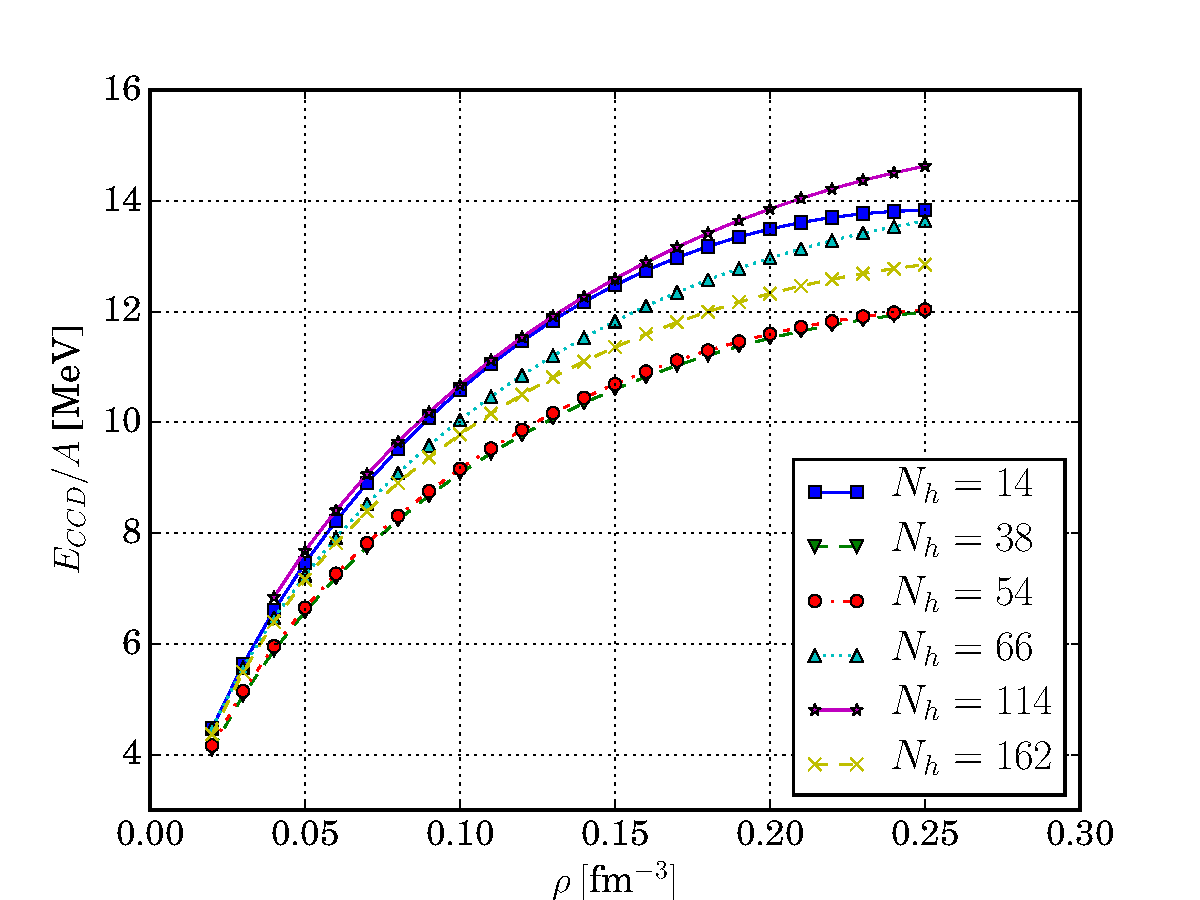
\includegraphics[width=0.7\textwidth]{Figures/MP_CCD_DENSITY_RUNS.pdf}
		\caption{Energies for the Minnesota potential in the CCD approximation using 40 shells (2042 states), as a function of density $\rho$.}
		\label{Implementation | fig | "MP rho dependency Ns=40"}
	\end{figure}
	
	In figure \ref{Implementation | fig | "MP state dependency"}, we show how the CCD energy from the Minnesota potential changes with the number of particles and states. This figure is quite important because we have found the CCDT energies to converge at the same rate as the CCD results as a function of state space size for all runs we have performed (see tables at the end of this chapter). This means that we may use CCD as a means to determine how many states we need to produce fairly stable results. Looking at the figure, we see that the various particle numbers will have converged results if we run with certain minimum states space sizes. Roughly, we see:
	
	\begin{center}
		\begin{tabular}{cl}
			$N_h$ & $N_s$ \\
			14 & $\geq$ 500 \\
			38 & $\geq$ 750 \\
			54 & $\geq$ 1500 \\
			66 & $\geq$ 1750 \\
			114 & $\geq$ 2000
		\end{tabular}
	\end{center}
	
	However, these values are for almost completely converged results. We can still do realistic calculations for smaller sizes, they just will not be absolutely converged. We say this because, even increasing the state space size by 100 means a lot for size of objects we have to store. For our calculations with 66 particles, we used a state space of 25 shells, or 1030 states, which is much lower than what we state above, but still fairly good when compared to the 66 particle line in figure \ref{Implementation | fig | "MP state dependency"}. This we had to do due to the limited time frame\footnote{The CCDT calculations do not take too long for reasonable densities, at most a week, but when they require so much memory we must use the Abel "hugemem" nodes. There are few such nodes available, and we needed to do many runs. Time efficiency was very necessary.} for performing analysis. We have relied much on this figure to predict state space sizes to do CCDT calculations.\\
	
	\begin{figure}[h]
		\centering
		\captionsetup{width=.8\textwidth}
		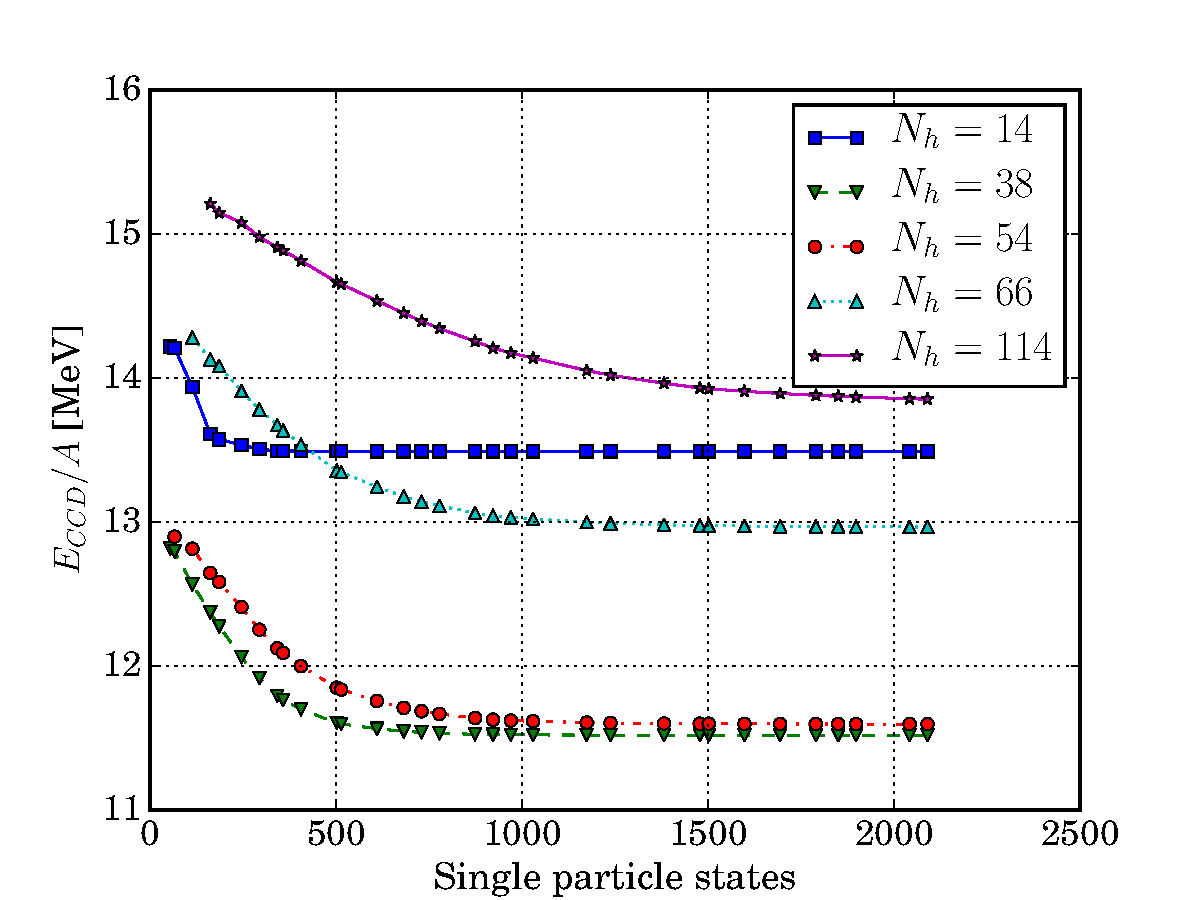
\includegraphics[width=0.7\textwidth]{Figures/MP_CCD_RUNS.pdf}
		\caption{Convergence of the CCD corrections to $E_{\text{ref}}$ for the Minnesota potential, as a function of state space size. The density here is $\rho=0.2\:\text{fm}^{-3}$.}
		\label{Implementation | fig | "MP state dependency"}
	\end{figure}
	
	We mentioned in chapter \ref{Int.Nucl.Mat.} that the Minnesota potential is a soft potential, meaning it is comparatively long-ranged. This is why, in figure \ref{Implementation | fig | "density for MP"}, we see the energy tends to even out after $\rho = 0.3\:\text{fm}^{-3}$. In \cite{GHagen14}, a similar CCD study of infinite neutron matter was done using the $\text{NNLO}_{\text{opt}}$ potential from which the interaction matrix elements across the Fermi surface is greater, and there they that found the energy density shows a different tendency beyond $\rho=0.15\:\text{fm}^{-3}$. While the Minnesota potential continues on a parabolic curve (decreasing gradient), the $\text{NNLO}_{\text{opt}}$ potential will instead change gradient such that it increases; a reflection of the "hardness" of the potential. Note that the due experimental data, the two nuclear potential should give very inconsistent data above $\rho=0.2\:\text{fm}^{-3}$, as we see in the density plots.
	
	\begin{figure}
		\centering
		\captionsetup{width=.8\textwidth}
		\hspace{0.35cm}
		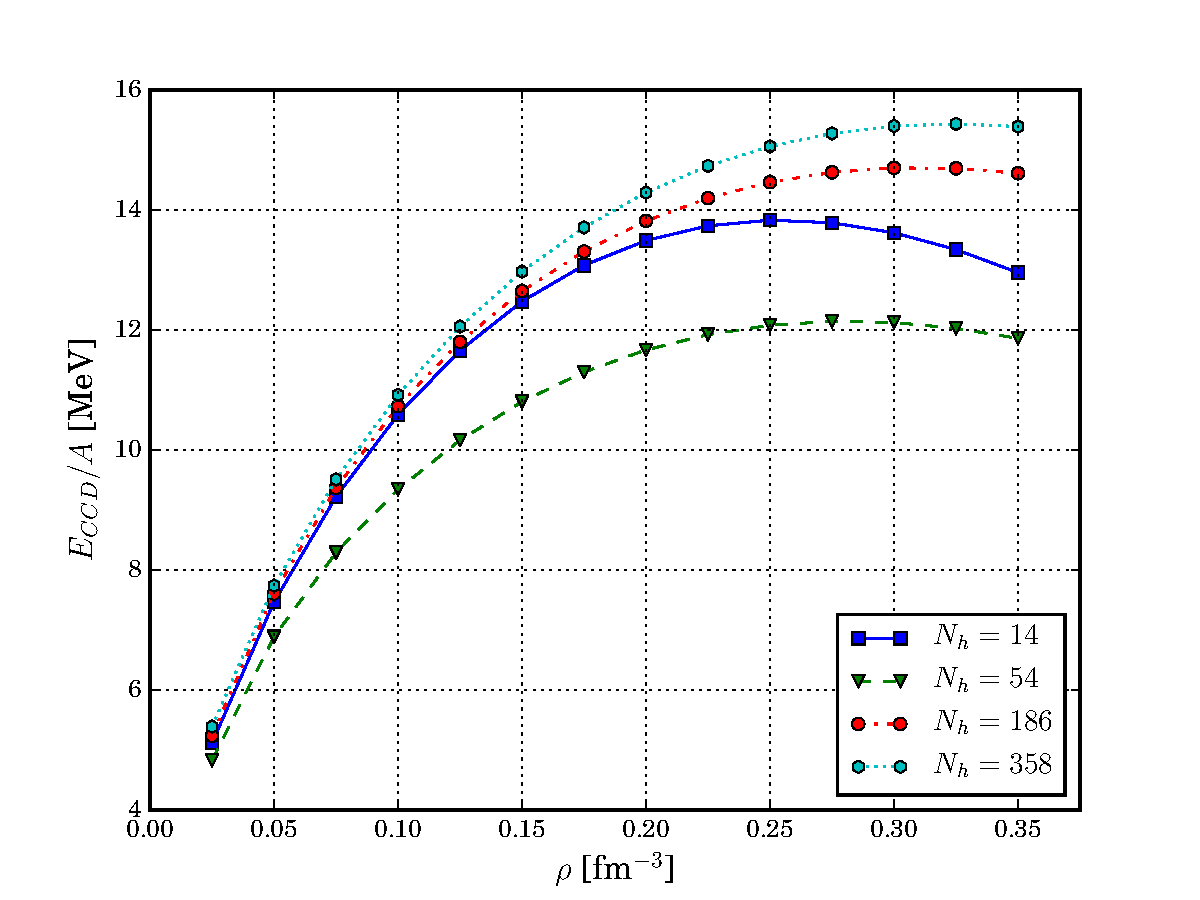
\includegraphics[width=0.81\textwidth]{Figures/density_for_MP.pdf}
		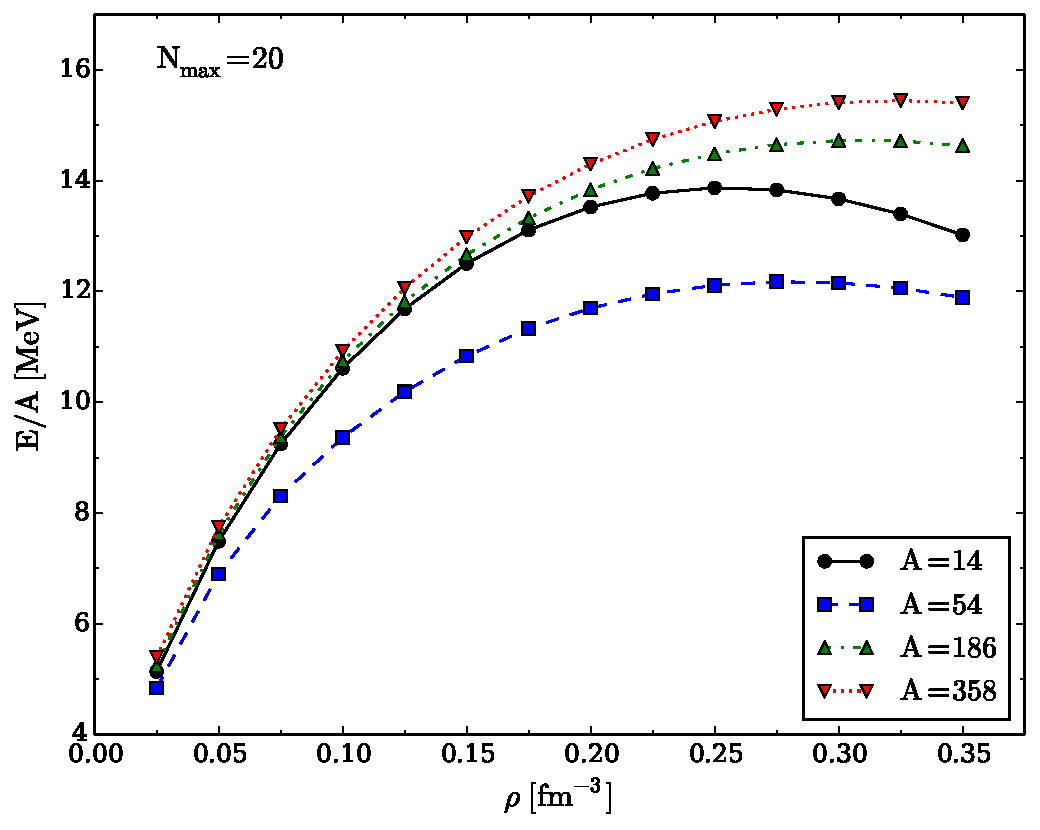
\includegraphics[width=0.7\textwidth]{Figures/nucl_comp_density_for_MP.pdf}
		\caption{Density and particle number dependency for the CCD corrections (top) to $E_{\text{ref}}$ for the Minnesota potential, with $N_b=20$, compared to the CCD corrections (bottom) from \cite{HJensenLombardoKolck16}.}
		\label{Implementation | fig | "density for MP"}
	\end{figure}
	\newpage
	
	\section{CCDT calculations}
	We now have CCD data with which to compare so we start introducing CCDT data. Since the CCDT calculations take far longer to perform than the CCD calculations, we had to be careful with the remaining time at our disposal. Therefore, our analysis may be somewhat limited, but we have still managed to include all the results necessary to see how CCDT can improve upon energy densities.\\
	
	Our first runs were mainly based on the HEG, where we wanted to see if CCDT had the same state space size dependency as CCD. Rather than plot the energy dependencies as we did in figure \ref{Implementation | fig | "MP rho dependency Ns=40"} for the Minnesota potential, we made tables. Primarily we did so such as to provide any future CCDT studies some benchmarks, but also so as to see exact values since graphs do not allow for such accuracy. In tables \ref{Appendix B | table | CCDT for HEG rs=0.5}, \ref{Appendix B | table | CCDT for HEG Nh14 rs=1.0}, \ref{Appendix B | table | CCDT for HEG rs=2.0}, and \ref{Appendix B | table | CCD for HEG Nh66 rs=1.0}, we provide CCDT* energies\footnote{Note that these are CCDT* energies. The tables were produced before we discovered the channel error in $T_{5a}$, but we have done several random checks to see the discrepancy. As already commented, the error in CCDT* compared to CCDT usually lies in the 4-7th decimal.}as a function of $N_s$ for $N_h=14$. We have chosen the same values for the Wigner-Seitz radius as those primarily seen in \cite{Hansen15}.\\
	
	Firstly, we see that the CCD and CCDT* columns converge at the same pace. Secondly, the CCDT* energies seem to behave inconsistently over densities, where the difference goes from $\sim 0.053s$ A.U. for $r_s=0.5$, $\sim 0.019$ A.U. for $r_s=1.0$, and $\sim 0.041$ A.U. for $r_s=2.0$.\\
	
	\newpage
	\begin{table}
		\centering
		\captionsetup{width=.8\textwidth}
		\caption{CCD and CCDT* for the HEG. Here, $N_h=14$ and $r_s = 0.5$. The CCD column is written with $10^{-16}$ precision, while the CCDT* columns are written with $10^{-15}$ precision.} %UP TO DATE AS OF 23/06/17
		\label{Appendix B | table | CCDT for HEG rs=0.5}
		\begin{tabular}{rrlll}
			Shells & States & $\Delta E_{CCD}$ [A.U.] & $\Delta E_{CCDT}$ [A.U.] & $E_{CCDT}/A$ [A.U.]\\
			%2 & 38 & -0.2916538151909717 & &\\ 
			3 & 54 & -0.3336006178979127 & -0.3613226307613434 & 4.1593823098206268\\ 
			4 & 66 & -0.414419044337637 & -0.4528623183396961 & 4.1528437607078876\\ 
			5 & 114 & -0.4723765026434803 & -0.5175111219244124 & 4.1482259890232651\\ 
			6-7 & 162 & -0.5062012474076132 & -0.5537431168067216 & 4.1456379893888142\\
			8 & 186 & -0.5114620616957333 & -0.5595831331786725 & 4.1452208453622470\\ 
			9 & 246 & -0.519428130833696 & -0.5686738314603959 & 4.1445715097706950\\ 
			10 & 294 & -0.5253668296623293 & -0.5753168603828068 & 4.1440970077048087\\ 
			11 & 342 & -0.5291183486696021 & -0.5796128140978349 & 4.1437901538680206\\ 
			12 & 358 & -0.5297417436322546 & -0.5803422346972473 & 4.1437380523966336\\ 
			13 & 406 & -0.5315206585936676 & -0.5824085916601776 & 4.1435904554707106\\ 
			14-15 & 502 & -0.5342063850776724 & -0.5855539088949929 & 4.1433657899539380\\ 
			16 & 514 & -0.5344264957627748 & -0.5858085751672242 & 4.1433475995059217\\
			17 & 610 & -0.5357789027540132 & -0.5873960344190747 & 4.1432342095593606\\
			18 & 682 & -0.5366472099813642 & -0.5884182562142592 & 4.1431611937168471\\ 
			19 & 730 & -0.5370975401996935 & -0.5889518934711170 & 4.1431230767699292\\ 
			20 & 778 & -0.5375047535914982 & -0.5894334589933603 & 4.1430886792326254\\ 
			21 & 874 & -0.5382050147446914 & -0.5902629204699491 & 4.1430294319842984\\ 
			22-23 & 922 & -0.5384573813567394 & -0.5905642205469669 & 4.1430079105502253\\ 
			24 & 970 & -0.5386710927147366 & -0.5908183744928200 & 4.1429897566969505\\ 
			25 & 1030 & -0.538885641914672 & -0.5910737828551182 & 4.1429715132425002\\ 
			26 & 1174 & -0.5393690537539687 & -0.5916496509829725 & 4.1429303798047963\\ 
			27-28 & 1238 & -0.5395547845509221 & -0.5918705963833766 & 4.1429145979904822\\ 
			29 & 1382 & -0.5398883846627222 & -0.5922701014597570 & 4.1428860619135977\\ 
			30-31 & 1478 & -0.5400978911472799 & -0.5925206017106548 & 4.1428681690385334\\
			32 & 1502 & -0.5401076152689156 & -0.5925640178197176 & 4.1428650678878860\\ 
			33 & 1598 & -0.5402794439784825 & -0.5927380408247316 & 4.1428526376732417\\ 
			34 & 1694 & -0.5404045196794176 & -0.5928883790387164 & 4.1428418992293858\\ 
			35 & 1790 & -0.5405320305355353 & -0.5930412649137533 & 4.1428309788097408\\ 
			36 & 1850 & -0.5405966801277755 & -0.5931190042506940 & 4.1428254259999591\\ 
			37 & 1898 & -0.5406429764745826 & -0.5931745238370971 & 4.1428214603152158\\ 
			38-39 & 2042 & -0.5407839652259617 & -0.5933437749858157 & 4.1428093709474503\\ 
			40 & 2090 & -0.5408224852237319 & -0.5933900700572950 & 4.1428060641566304\\ 
		\end{tabular}
	\end{table}
	\newpage
	
	\begin{table}
		\centering
		\captionsetup{width=.8\textwidth}
		\caption{CCD and CCDT* for the HEG. Here, $N_h=14$ and $r_s = 1.0$. The CCD column is written with $10^{-16}$ precision, while the CCDT* columns are written with $10^{-15}$ precision.} %UP TO DATE AS OF 23/06/17
		\begin{tabular}{rrlll}
			Shells & States & $\Delta E_{CCD}$ [A.U.] & $\Delta E_{CCDT}$ [A.U.] & $E_{CCDT}/A$ [A.U.] \\
			3 & 54 & -0.3178228436889337 & -0.3250227149973082 & 0.9484667586119215\\ 
			4 & 66 & -0.3926965898061971 & -0.4017914206413200 & 0.9429832796373493\\ 
			5 & 114 & -0.4479105961757173 & -0.4639628744093380 & 0.9385424615110622\\
			6-7 & 162 & -0.4805572589306421 & -0.4981036081719917 & 0.9361038376708727\\ 
			8 & 186 & -0.4855229317521322 & -0.5033237253884906 & 0.9357309721554085\\ 
			9 & 246 & -0.4929245740023971 & -0.5112376622762492 & 0.9351656909491400\\ 
			10 & 294 & -0.4984909094066807 & -0.5170296611136175 & 0.9347519767464708\\ 
			11 & 342 & -0.5019526761547779 & -0.5206479107639055 & 0.9344935303428789\\ 
			12 & 358 & -0.5025196736076418 & -0.5212432746002467 & 0.9344510043545687\\ 
			13 & 406 & -0.5041428350347078 & -0.5229285143935067 & 0.9343306300836216\\ 
			14-15 & 502 & -0.5065799526614782 & -0.5254622448103232 & 0.9341496493395633\\
			16 & 514 & -0.5067813814087071 & -0.5256708402523005 & 0.9341347496651363\\
			17 & 610 & -0.508005750884933 & -0.5269377732911092 & 0.9340442544480786\\ 
			18 & 682 & -0.5087901054753002 & -0.5277484754381196 & 0.9339863471518636\\ 
			19 & 730 & -0.5091947506340663 & -0.5281656225914414 & 0.9339565509266263\\ 
			20 & 778 & -0.5095611843521084 & -0.5285428325301044 & 0.9339296073595789\\ 
			21 & 874 & -0.5101903217891602 & -0.5291895772339356 & 0.9338834113093053\\ 
			22-23 & 922 & -0.5104161052303942 & -0.5294230952722792 & 0.9338667314494237\\ 
			24 & 970 & -0.510607489568679 & -0.5296193900471847 & 0.9338527103940732\\ 
			25 & 1030 & -0.510799565415577 & -0.5298165202968051 & 0.9338386296619575\\ 
			26 & 1174 & -0.5112320650410026 & -0.5302603149379534 & 0.9338069300447326\\ 
			27-28 & 1238 & -0.5113982335228359 & -0.5304295748884436 & 0.9337948400482690\\ 
			29 & 1382 & -0.5116958244765315 & -0.5307363423209762 & 0.9337729280888024\\ 
			30-31 & 1478 & -0.5118827825224076 & -0.5309280826928229 & 0.9337592323479562\\ 
			32 & 1502 & -0.5118882958571468 & -0.5309610396616040 & 0.9337568782787576\\ 
			33 & 1598 & -0.5120444603468518 & -0.5310933613048517 & 0.9337474267328113\\ 
			34 & 1694 & -0.5121557267166419 & -0.5312075816120850 & 0.9337392681394375\\ 
			35 & 1790 & -0.512269185709006 & -0.5313234396768680 & 0.9337309925633815\\ 
			36 & 1850 & -0.512326660011779 & -0.5313824002158976 & 0.9337267810963079\\ 
			37 & 1898 & -0.5123678973750974 & -0.5314246834331559 & 0.9337237608665038\\ 
			38-39 & 2042 & -0.5124932715755394 & -0.5315528087238279 & 0.9337146090600272\\ 
			40 & 2090 & -0.5125274988976634 & -0.5315877533729573 & 0.9337121130136609\\ 
		\end{tabular}
		\label{Appendix B | table | CCDT for HEG Nh14 rs=1.0}
	\end{table}
	\newpage
	
	\begin{table}
		\centering
		\captionsetup{width=.8\textwidth}
		\caption{CCD and CCDT* for the HEG. Here, $N_h=14$ and $r_s = 2.0$. The CCD column is written with $10^{-16}$ precision, while the CCDT* columns are written with $10^{-15}$ precision.} %UP TO DATE AS OF 23/06/17
		\begin{tabular}{rrlll}
			Shells & States & $\Delta E_{CCD}$ [A.U.] & $\Delta E_{CCDT}$  & $E_{CCDT}/A$ [A.U.]\\
			%2 & 38 & -0.2204456034603233 &  & \\ 
			3 & 54 & -0.2589156130047479 & -0.2770837947289984 & 0.1858214168509207\\ 
			4 & 66 & -0.3134082887534794 & -0.3357455207538542 & 0.1816312935634310\\ 
			5 & 114 & -0.3577968843144998 & -0.3954097545082366 & 0.1773695625809751\\ 
			6-7 & 162 & -0.3855831022718813 & -0.4249223676995542 & 0.1752615187815952\\
			8 & 186 & -0.3894387566079127 & -0.4291166342209300 & 0.1749619283157827\\ 
			9 & 246 & -0.3947792888409713 & -0.4352451596266133 & 0.1745241765010910\\ 
			10 & 294 & -0.3989857639655908 & -0.4396989645522079 & 0.1742060475778343\\ 
			11 & 342 & -0.4014136184665562 & -0.4423155241342955 & 0.1740191504648280\\ 
			12 & 358 & -0.4017831726474924 & -0.4427203216709363 & 0.1739902363550680\\ 
			13 & 406 & -0.4028646373532681 & -0.4438680944764375 & 0.1739082525832464\\ 
			14-15 & 502 & -0.4044444160771550 & -0.4455512648002199 & 0.1737880261315477\\ 
			16 & 514 & -0.4045812896518079 & -0.4456951627302880 & 0.1737777477079714\\ %62876s
			17 & 610 & -0.4053686959017509 & -0.4465239093301989 & 0.1737185515222635\\ 
			18 & 682 & -0.4058682250906545 & -0.4470481074978307 & 0.1736811087960040\\ 
			19 & 730 & -0.4061192159485590 & -0.4473098524427287 & 0.1736624127285114\\ 
			20 & 778 & -0.4063488815130470 & -0.4475483645304318 & 0.1736453761508183\\ 
			21 & 874 & -0.4067397467310569 & -0.4479529001526972 & 0.1736164807492279\\ 
			22-23 & 922 & -0.4068770351672458 & -0.4480972932081725 & 0.1736061669595511\\ 
			24 & 970 & -0.4069941779278041 & -0.4482178727943892 & 0.1735975541319641\\ 
			25 & 1030 & -0.4071118562687619 & -0.4483392192035621 & 0.1735888865313089\\ 
			26 & 1174 & -0.4073757859564262 & -0.4486113047906565 & 0.1735694518465165\\ 
			27-28 & 1238 & -0.4074771613061054 & -0.4487112188244932 & 0.1735623151298139\\ 
			29 & 1382 & -0.4076563555449695 & -0.4489007806420157 & 0.1735487749999909\\ 
			30-31 & 1478 & -0.4077691604146162 & -0.4490168948544763 & 0.1735404811276722\\
			32 & 1502 & -0.4077883408936130 & -0.4490365455038302 & 0.1735390775098613\\ 
			33 & 1598 & -0.4078657146012820 & -0.4491156363639367 & 0.1735334281627108\\ 
			34 & 1694 & -0.4079319552545511 & -0.4491839092200833 & 0.1735285515301289\\ 
			35 & 1790 & -0.4079995270290966 & &\\ 
			36 & 1850 & -0.4080336209247829 & &\\ 
			37 & 1898 & -0.4080583547955437 & -0.4493133415771160 & 0.1735193063617694\\ 
			38-39 & 2042 & -0.4081328308166824 & &\\ 
			40 & 2090 & -0.4081531318998730 & &\\ 
		\end{tabular}
		\label{Appendix B | table | CCDT for HEG rs=2.0}
	\end{table}
	
	\newpage
	

	In figure \ref{Results | fig | "MP CCD CCDT comparison, Nh=14, Nb=18"}, we show the energy density for 14 neutrons with the Minnesota potential, with 682 states (18 shells), for both the CCD and CCDT approximations. The CCDT contributions appear to have larger effects for densities below the neutron saturation density. Increasing the number of particles to 38, we see figure \ref{Results | fig | "MP CCD CCDT comparison, Nh=38, Nb=16"}. Here we could only run with 514 states (16 shells) due to the error we experienced with the \texttt{ppmm\_pphh} index matrix. Such a small states space means that, according to figure \ref{Implementation | fig | "MP state dependency"}, the energy is not yet expected to converge.\\
		
	However, since the CCD and CCDT energies apparently converge at the same rate, we may expect a discrepancy from the true CCDT results that is similar to the one of CCD\footnote{At first glance, this seems to be about 0.8\% from the true $N_h=38$ CCDT energy.}. For $N_h=38$, the CCD and CCDT energies are very nearly the same. Due to the significant different natures of the 14 and 38 neutron cases, we expect there is a need to include higher particle numbers. After all, the CCD analysis in figure \ref{Implementation | fig | "MP rho dependency Ns=40"} suggests so. There, the 14 and 38 particle cases are the most different of all the curves. It is, however, quite interesting that this has an effect on the CCDT corrections. We show the ratios of the curves from \ref{Implementation | fig | "MP state dependency"} in figure \ref{Results | fig | "MP CCD CCDT comparison ratio, Nh=38, Nb=16"}.\\
		
	Finally, we calculated the CCDT correlation energies for the $\text{NLO2}_{\text{opt}}$ potential, shown in figure \ref{Results | fig | "CHIRAL CCD CCDT comparison, Nh=14, Nb=18"}, for 14 particles and 18 shells. These results are temporary, and we expect far better results in results later studies \cite{MillerHjorthJensen17}. There have already been an extensive analysis of the potential performed in \cite{GHagen14} in the CCD approximation, and we expect interesting effects to be seen by the inclusion of a CCDT approximation. This, mainly, due to the effect CCDT apparently has in densities below neutron condensate.\\
	
	Before concluding this chapter, we present table \ref{Appendix B | table | CCD for MP}, where the dependency of the Minnesota potential on state space size can be seen for 14 neutrons.
	
	
	\begin{figure}
		\centering
		\captionsetup{width=.8\textwidth}
		\hspace{0.35cm}
		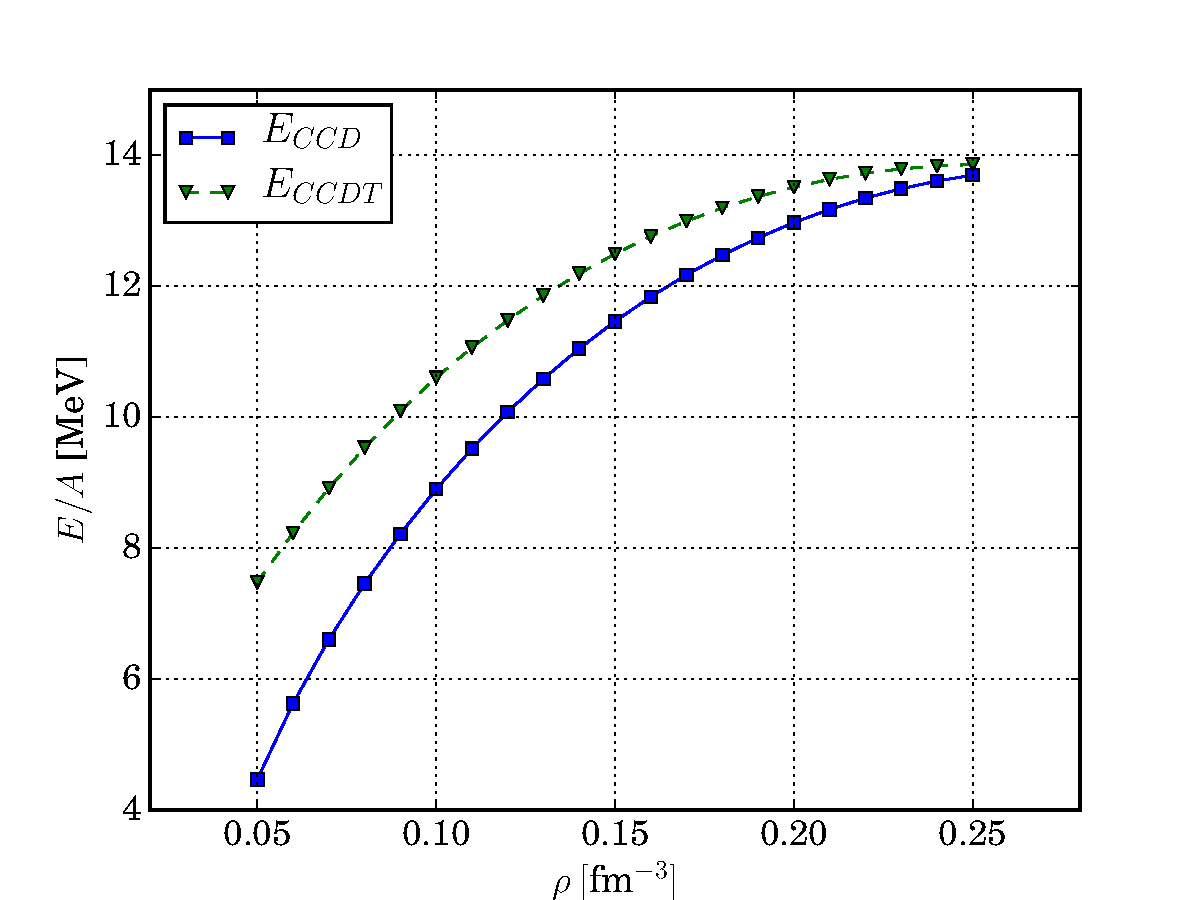
\includegraphics[width=0.7\textwidth]{Figures/MP_CCDT_COMPARISON.pdf}
		\caption{CCD and CCDT energies for the Minnesota potential, for $N_h=14$ and $N_s=682$ (18 shells).}
		\label{Results | fig | "MP CCD CCDT comparison, Nh=14, Nb=18"}
	\end{figure}
	
	\begin{figure}
		\centering
		\captionsetup{width=.8\textwidth}
		\hspace{0.35cm}
		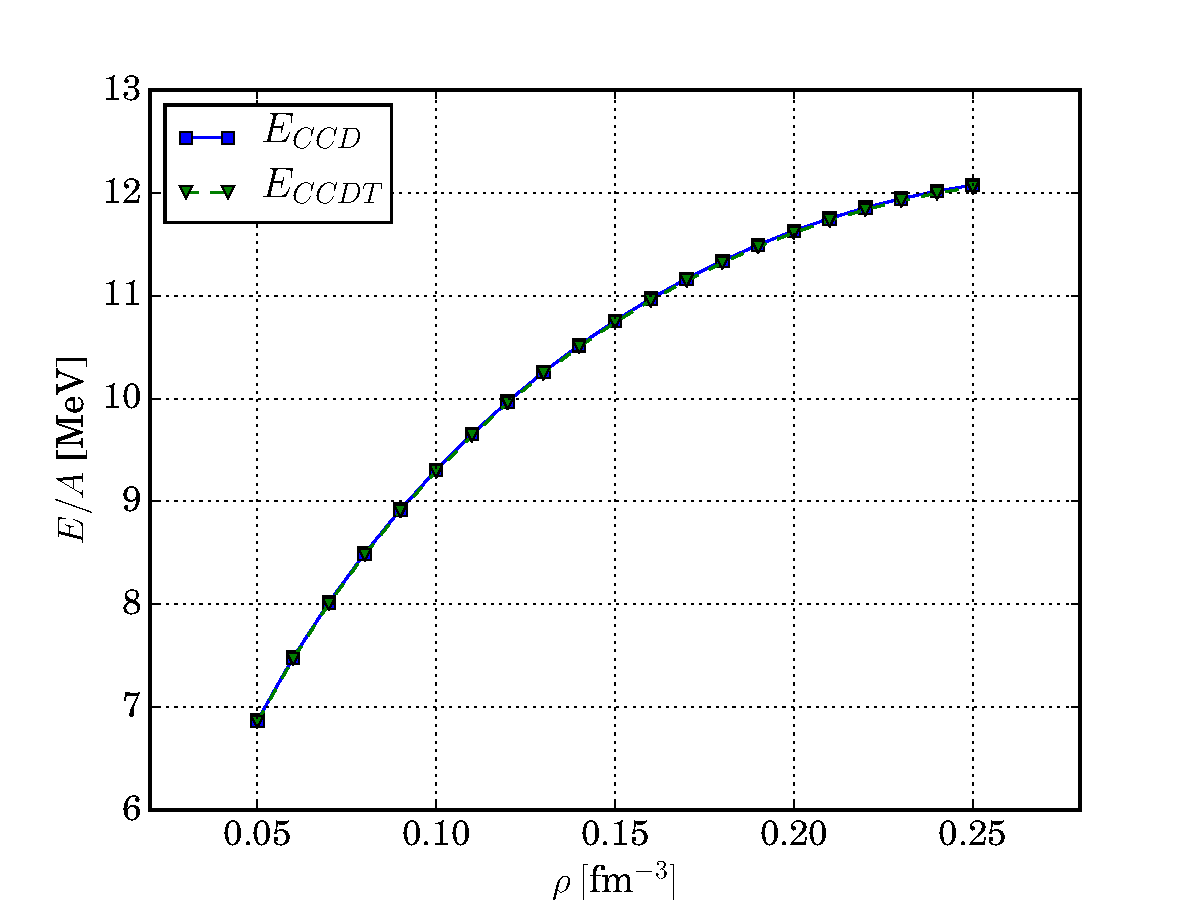
\includegraphics[width=0.7\textwidth]{Figures/MP_CCDT_COMPARISON_NH38.pdf}
		\caption{CCD and CCDT energies for the Minnesota potential, for $N_h=38$ and $N_s=514$ (16 shells).}
		\label{Results | fig | "MP CCD CCDT comparison, Nh=38, Nb=16"}
	\end{figure}
	
	\begin{figure}
		\centering
		\captionsetup{width=.8\textwidth}
		\hspace{0.35cm}
		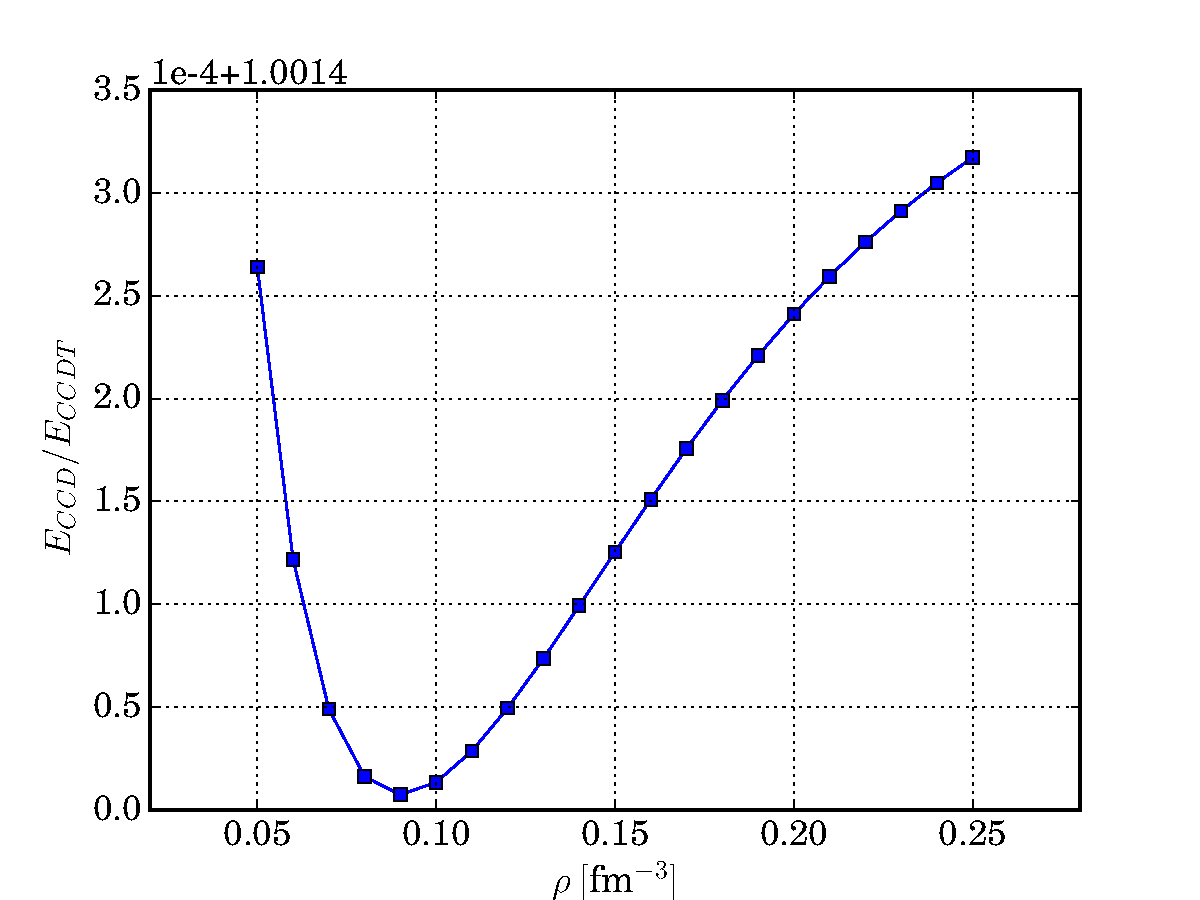
\includegraphics[width=0.7\textwidth]{Figures/MP_CCDT_COMPARISON_NH38_RATIO.pdf}
		\caption{The ratio $\frac{E_{\text{CCD}}}{E_{\text{CCDT}}}$ from figure \ref{Results | fig | "MP CCD CCDT comparison, Nh=38, Nb=16"}, for $N_h=38$ and $N_s=514$ (16 shells).}
		\label{Results | fig | "MP CCD CCDT comparison ratio, Nh=38, Nb=16"}
	\end{figure}
	
	\begin{figure}
		\centering
		\captionsetup{width=.8\textwidth}
		\hspace{0.35cm}
		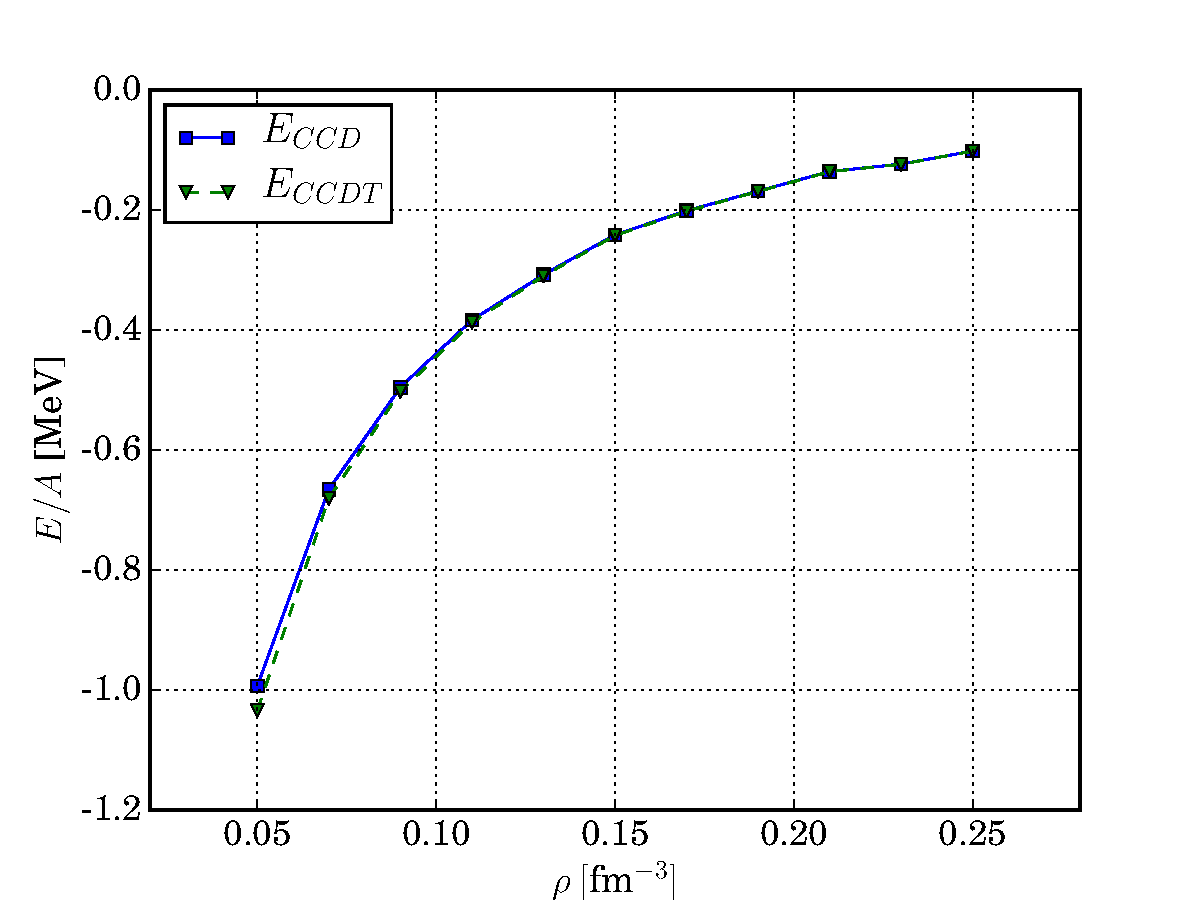
\includegraphics[width=0.7\textwidth]{Figures/CHIRAL_CCDT_COMPARISON.pdf}
		\caption{CCD and CCDT correlation energies for the $\text{NLO2}_{\text{opt}}$ potential, for $N_h=14$ and $N_s=682$ (18 shells).}
		\label{Results | fig | "CHIRAL CCD CCDT comparison, Nh=14, Nb=18"}
	\end{figure}
	
	\begin{table}[h]
		\centering
		\captionsetup{width=.8\textwidth}
		\caption{CCD and CCDT for the Minnesota potential in pure neutron matter. Here, $N_h=14$, $\rho = 0.2$, and $E_{\text{ref}}=204.9471889302268$ MeV. The CCD column is written with $10^{-15}$ precision, and CCDT with $10^{-10}$ precision for $N_b\in[2,16]$, and $10^{-7}$ precision for $N_b>16$.}
		\begin{tabular}{rrlll}
			Shells & States & $\Delta E_{CCD}$ [MeV] & $\Delta E_{CCDT}$ [MeV] & $E_{CCDT}/A$ [MeV]\\
			%2 & 38 & -2.3084208310110648 &  &\\ 
			3 & 54 & -5.884775823948868 & -5.58788023 & 14.2399345\\ 
			4 & 66 & -6.035987745077961 & -5.74503030 & 14.2287095\\ 
			5 & 114 & -9.841615786590484 & -9.52325124 & 13.9588526\\ 
			6-7 & 162 & -14.386077965543356 & -14.0073939 & 13.6385567\\ 
			8 & 186 & -14.903996242309114 & -14.5293199 & 13.6012763\\ 
			9 & 246 & -15.469112996657206 & -15.1022748 & 13.5603510\\ 
			10 & 294 & -15.867026079093812 & -15.5035885 & 13.5316857\\ 
			11 & 342 & -16.02672117326827 & -15.6659251 & 13.5200902\\ 
			12 & 358 & -16.033336357473196 & -15.6733595 & 13.5195592\\ 
			13 & 406 & -16.05300799553373 & -15.6943706 & 13.5180584\\ 
			14-15 & 502 & -16.065386808567148 & -15.7085730 & 13.5170439\\ 
			16 & 514 & -16.066710716629423 & -15.7099731 & 13.5169439\\
			17 & 610 & -16.06854213668595 & -15.7123620 & 13.5167733\\ 
			18 & 682 & -16.06905842272527 & -15.7131474 & 13.5167172\\ 
			19 & 730 & -16.069139521294144 & -15.7133543 & 13.5167024\\ 
			20 & 778 & -16.06919444582676 & -15.7134939 & 13.5166924\\
			21 & 874 & -16.069305317310093 & -15.7137386 & 13.5166750\\ 
			22-23 & 922 & -16.06939452350382 & -15.7138695 & 13.5166656\\ 
			24 & 970 & -16.069440546944495 & -15.7139377 & 13.5166607\\ 
			25 & 1030 & -16.06947503042378 & -15.7139866 & 13.5166573\\ 
			26 & 1174 & -16.069539570489834 & -15.7140758 & 13.5166509\\ 
			27-28 & 1238 & -16.06955902670211 & -15.7141029 & 13.5166490\\ 
			29 & 1382 & -16.069585105093047 & -15.7141365 & 13.5166465\\ 
			30-31 & 1478 & -16.06959737262169 & -15.7141525 & 13.5166454\\ 
			32 & 1502 & -16.069598629666043 & -15.7141540 & 13.5166453\\ 
			33 & 1598 & -16.06960222976907 & -15.7141586 & 13.5166450\\ 
			34 & 1694 & -16.06960442793497 & -15.7141613 & 13.5166448\\ 
			35 & 1790 & -16.069606029815077 & -15.7141632 & 13.5166446\\ 
			36 & 1850 & -16.069606604957954 & -15.7141640 & 13.5166446\\ 
			37 & 1898 & -16.069607071806754 & -15.7141645 & 13.5166445\\ 
			38-39 & 2042 & -16.069607755038646 & -15.7141654 & 13.5166445\\ 
			40 & 2090 & -16.069607874446504 & -15.7141656 & 13.5166445\\
			41 & 2282 & -16.06960808837813 &&
		\end{tabular}
		\label{Appendix B | table | CCD for MP}
	\end{table}
	
	\chapter{Conclusions and future prospects}
	
	While our analyses are not fitting for estimates of thermodynamic properties of infinite matter, they have shown that including full CCDT correlations does change the energy density, especially for densities where the Minnesota potential is well defined experimentally (below neutron condensate). This, together with the fact that the Minnesota potential and the $\text{NLO2}_{\text{opt}}$ \cite{HJensenEtAl13} potentials differ in the medium density range ($\rho\geq 0.15\:\text{fm}^{-3}$) \cite{GHagen14} means that we expect interesting effects from running a full CCDT analysis for $\text{NLO2}_{\text{opt}}$. However, such would have to be with a bigger number of particles and necessary state space size for convergence of energies, than contained herein.\\
	
	We found that low-density analysis for the HEG was difficult. For a Wigner-Seitz radius $r_s\geq 2.0$, the CC method uses very many steps to converge. This severely restricted a CCDT calculation for such systems. However, we managed a state space dependency test for radii $r_s=0.5,\: 1.0$, and 2.0. The Minnesota potential, on the other hand, behaved very nicely in the density ranges it is well defined. this bodes well for calculations with higher particle numbers.\\
	
	The main body of work in thesis has provided us with a general programme that allows us to perform further, more advanced studies of the homogeneous electron gas and infinite nuclear matter. It is believed that this work shall be built upon to perform a more in-depth CCDT calculation and analysis of neutron star matter by S.B.S. Miller and M. Hjorth-Jensen in the near future. We believe a more realistic CCDT calculation should be achievable using a twist-average boundary condition (TABC). TABC has been shown \cite{HJensenLombardoKolck16} to correct for the finite size effects for the Minnesota potential, and have worked well for analysis of nuclear matter with chiral potentials \cite{GHagen14}.\\
	
	The programme has taken a long time to develop, and it is unique for such an implementation to be written by a single author. It is written in a general class structure, allowing for easy implementation of new system classes; classes that hold the details of the system state space, quantum numbers, and one- and two-body interactions. It is our hope that the programme shall be used further, not just for a single paper \cite{MillerHjorthJensen17}, but for several analyses with new potentials. With the application of lattice quantum chromodynamics becoming more and more accessible, we expect to see an increased need for the knowledge and skill to unify lattice quantum chromodynamics with chiral effective field theory. Using these two together brings about the possibility to use very realistic nucleon-nucleon potentials in many-body, nuclear systems. We hope this programme will serve as a foundation to apply those potentials, to gain high precision results.\\
	
	\newpage
	
	Lastly, we comment on the specific details of further study. Firstly, extending this work to use twist-averaged boundary conditions is believed would correct finite-sized effects a great deal, as it did in \cite{GHagen14}. We note that having included such an analysis, together with a general study of finite-size effects, is far past the scope of this thesis. Another topic of interest to study would be to improve upon this implementation to consider even larger numbers of particles and larger state space sizes. Due to the nature of the nuclear force, we do not expect such an analysis would require very many particles, but the state space dependency is more uncertain, hence the interest.
	
	\newpage
	\begin{appendices}
	\chapter{Lie groups}\label{Appendic A | Lie groups}
	Lie groups have a huge range of applications in physics, and no appendix can possibly do the topic justice. Fortunately, we do not need to. We only need an intuitive, although perhaps naive, understanding of Lie groups in order to use them. We are certain the reader will find little difficulty in finding a more in-depth introduction elsewhere, should they so desire. The mathematics presented herein is in inspired by \cite{Nakahara}.\\
	
	Lie groups are a combination of two mathematical concepts, one being \emph{groups} and the other being \emph{differentiable manifolds}. The former provides a way to define an operation between two elements of a set of elements, like, for example, arithmetic on the real line ($\mathbb{R}$). The latter tells us how to describe, in Euclidean coordinates, a continuous movement (transformation) across an object. If we then combine the two concepts, we get a tool that allows us to continuously transform quantities. What, exactly, these quantities are, we shall give examples of soon. So to define a Lie group, we need to define groups and differentiable manifolds.
	
	\subsection{Manifolds}
	\subsubsection{Topological spaces}
	Before even defining a manifold, we need to have an understanding of so-called \emph{topological spaces}. While there are several equivalent definitions, we will use the "open set" definition. So, a topological space is an ordered pair $(S,\tau)$, where $S$ is a set and $\tau$ is a collection of all \emph{open} subsets of $S$, satisfying that:
	
	\begin{enumerate}
		\item the empty set $\emptyset$ and the full set $S$ are members of $\tau$: $\emptyset, S\in \tau$
		\item any union of sets in $\tau$ is still within $\tau$: $\left\{\bigcup_\alpha U_\alpha\in\tau\: \forall \:U_\alpha\in\tau\right\}$ 
		\item intersections of any finite number of sets in $\tau$ is still within $\tau$: $\left\{U\bigcap V\in\tau\: \forall \:U,V\in\tau\right\}$ 
	\end{enumerate}
	
	It is called "open set" because the set is just that; open. There is no boundary which restricts the members of $\tau$, they are fully self-contained. An element $x\in S$ has \emph{neighbourhood} $U_\alpha$ if $x\in U_\alpha$. With this sense of neighbourhoods, it gets easier to understand why we call it a \emph{topological} space. Topology is the mathematical study of shapes, and if we know where points are in respect to each other via neighbourhoods of points within some well-defined set $S$ of points, we can construct a "shape". Of course, we shall be a bit more mathematically formal than this.
	
	\subsubsection{Charts}
	In addition to topological spaces, a manifold requires a so-called \emph{atlas}, which is a collection of \emph{charts}. These charts are what allows us to describe translations on the manifold by the use of coordinate systems.\\
	Given two sets, we may define a mapping between the members of the two sets. For example, let's say we have two sets $A = \{a_1,a_2,a_3,a_4\}$ and $B = \{b_1,b_2,b_3,b_4\}$, and a map $\phi: A \to B$ such that $\phi: a_i\mapsto b_i$. We then call $\phi$ a map from $A$ to $B$. Immediately this reminds us of functions; given a member $x \in \mathbb{R}$, we get a value $f(x) \in \mathbb{R}$. If we call the subset of $\mathbb{R}$ spanned by $f(x)$ for $\mathbb{F}$, then we could say $f$ is our map, and
	
	\begin{equation}
	f: \mathbb{R} \to \mathbb{F} \:.
	\end{equation}
	
	Given this simple concept, we will need some terms that describe the details of a map. Let us call the set we map \emph{from} for the domain, and the set we map \emph{to} for the co-domain. All maps fall into one of the following classifications:
	
	\begin{enumerate}
		\item Surjective: Every member of the co-domain is mapped onto at least once, such that all members of the domain have been mapped, but may share mapping. That is, the map is one-to-one.
		\item Injective: Every member of the domain is mapped into the co-domain, such that all members of the domain have been mapped and do not share mapping. That is, the map is onto.
		\item Bijective: All members of the domain are mapped uniquely onto all members of the co-domain, giving a one-to-one correspondence between the two domains. That is, the map is both onto and one-to-one.
	\end{enumerate}
	
	All maps we speak of will be bijective, such that there will be no "overlap" between members. Only bijective maps have a well-defined inverse map $\phi^{-1}$, going from the co-domain back to the domain.\\
	
	As we know, translations (in time, space, momentum, etc) are smooth movements. For example, walking across the Earth means smoothly moving from one set member to the next. However, we need a precise definition of smoothness. That is where \emph{continuous maps} come into play. Defining continuous maps is very simple. We say a map $\phi: S\rightarrow S'$ is continuous if for any open set $U' \subseteq S'$, the complementary set $U\subseteq S$ is an open set. It might seems curious as to why continuity is defined by inverse mapping, but it is very natural when considering functions as we know them.\\
	
	As mentioned earlier, a function takes one set of values and produces another, which is why it has very much to do with maps. However, functions as we normally consider them are defined in a coordinate system, whereas a topological space is not. 
	
	\subsubsection{Manifolds}
	A $n$-dimensional manifold $M$ is a topological space that locally can be mapped to a Euclidean space $\mathbb{R}^n$. That is, we may divide our manifold into open sets $U_\alpha$ ($\bigcap_\alpha U_\alpha = M$), and map each set to $\mathbb{R}^n$, i.e.
	
	\begin{equation}
	\phi_\alpha: U_\alpha \rightarrow \mathbb{R}^n \:.
	\end{equation}
	
	We can also work with manifolds that have another property called \emph{differentiability}. If, for any two open sets $U_\alpha$ and $U_\beta$, the \emph{transition function} $\phi_\alpha \circ \phi_\beta^{-1}$ is differentiable, we have a differentiable manifold. We call our manifold a $C^k$-manifold if the transition function is $k$-times differentiable. We call it a \emph{smooth} manifold if it is a $C^\infty$-manifold. The set of all these charts is called the atlas of $M$.
	
	It is often helpful to imagine this with the surface of the Earth as our manifold (which would be a 2-sphere; $S^2$), and we can easily portray an area around a point with a Euclidean coordinate system, such as a city. However, our coordinate system fails to cover the entire sphere\footnote{You can go in one direction and come back to where you started. In $\mathbb{R}^3$, moving in one direction means you will simply move towards infinity, and never coming back to where you started.}.\\
	
	\subsection{Groups}
	\emph{Groups} are one of the simplest mathematical objects we can have, preceded perhaps only by sets. A group is a set with operations, usually written $G=\{S,\cdot\}$ ($S$ being the set and $(\cdot)$ the operation), that must satisfy 4 axioms.
	
	\begin{enumerate}
		\item \emph{Closure}: For the operation $a\cdot b=c$, with $a,b\in G$, we must have $c\in G$ as well.
		\item \emph{Associativity}: $a\cdot(b\cdot c) = (a\cdot b)\cdot c$
		\item \emph{Identity}: There exist a unique element $e$, called the \emph{identity}, for which we have $e\cdot a= a\cdot e = a \:\forall a\in\: S$.
		\item \emph{Inverse}: For every set member $a$, there is also an inverse set member $a^{-1}$ such that $a\cdot a^{-1} = a^{-1}\cdot a = e$.
	\end{enumerate}
	
	\subsection{Lie groups}
	The simplest way to think of a Lie group is as a smooth, differentiable manifold where the members abide by group operations. However, there are \emph{very} many properties included in this phrasing, so perhaps a more rigorous definition is needed. A Lie group is both a group and a manifold; a manifold with group properties that lets one "move about", or a group where multiplication and inversion are smooth maps. There are a few ways of thinking about Lie groups, but the mathematical definition is a smooth, differentiable manifold $G$ where the group operations multiplication ($\cdot$) and inversion ($g^{-1}$) are smooth maps, such that \cite{Nakahara}\\
	
	\begin{align}
		&\cdot \: : \: G\times G \rightarrow G\:,\quad (g_1,g_2)\mapsto g_1\cdot g_2 \\
		&\:^{-1} \: : \: G \rightarrow G\:,\quad g\mapsto g^{-1}
	\end{align}
	
	We shall refer the reader to \cite{Nakahara} for further discussion on the application of the Lie group. As we mentioned, however, Lie groups do not play a more fundamental role to us other than provide an intuitive way to imagine the transformation of gauge fields.
	
	\end{appendices}
	
	
	\begin{thebibliography}{9}
		
		\bibitem{MHjorthJensenHeiselberg00}
		H. Heiselberg and M. Hjorth-Jensen, \emph{Phases of Dense Matter in Neutron Stars}, Physics Reports 328, 237-327, 2000
		
		\bibitem{ShapiroTeukolsky83}
		S.L. Shapiro and S.A. Teukolsky, \emph{
			Black Holes, White Dwarfs and Neutron Stars: The Physics of Compact Objects}, 1st edition, Wiley-VCH, 1983
		
		\bibitem{ShavittBartlett09}
		I. Shavitt and R.J. Bartlett,
		\emph{Many-Body Methods in Chemistry and Physics}, Cambridge University Press, 2009
		
		\bibitem{MachleidtEntem11}
		R. Machleidt and D.R. Entem, \emph{Chiral effective field theory and nuclear forces}, Physics Reports 503, 1-75, 2011
		
		\bibitem{MillerHjorthJensen17}
		S.B.S. Miller and M. Hjorth-Jensen, In preparation, 2017
		
		\bibitem{HJensenEtAl13}
		A. Ekstr\"om, G. Baardsen, C. Forss\'{e}n, G. Hagen, M. Hjorth-Jensen, G.R. Jansen, R. Machleidt, W. Nazarewicz, T. Papenbrock, J. Sarich, and S.M. Wild, \emph{Optimized Chiral Nucleon-Nucleon Interaction at Next-to-Next-to-Leading Order}, Physical Review Letters 110, 192502, 2013
		
		\bibitem{Neumann32}
		J. von Neumann, \emph{Mathematical Foundations of Quantum Mechanics}, 1st edition, Princeton University Press, 1955
		
		\bibitem{Hansen15}
		A.S. Hansen,
		\emph{Coupled cluster studies of infinite systems} (Master's thesis), University of Oslo, 2015.
		
		\bibitem{Holmen16}
		F.W. Holmen,
		\emph{A Study of Coupled-Cluster Methods for Infinite Matter} (Master's thesis), University of Oslo, 2016
		
		\bibitem{Baardsen14}
		G. Baardsen, \emph{Coupled-cluster theory for infinite matter}  (Doctoral dissertation), University of Oslo, 2014
		
		\bibitem{PeskinSchroeder}
		M.E. Peskin and D.V. Schroeder, \emph{An Introduction to Quantum Field Theory}, Westview Press, 1995
		
		\bibitem{Weinberg95}
		S. Weinberg, \emph{The quantum theory of fields : Vol. 1 : Foundations}, Cambridge University Press, 1995
		
		\bibitem{Georgi84}
		H. Georgi, \emph{Weak Interactions and Modern Particle Theory}, Menlo Park, Calif. : Benjamin/Cummings Pub. Co., 1984
		
		\bibitem{SchererSchingler12}
		S. Scherer and M.R. Schindler, \emph{A Primer for Chiral Perturbation Theory}, Heidelberg ; New York : Springer, 2012.
		
		\bibitem{GrossRungeHeinonen91}
		E.K.U. Gross, E. Runge, and O. Heinonen, \emph{Many-Particle Theory}, Adam Hilger imprint by IOP Publishing Ltd, 1991
		
		\bibitem{HJensenLombardoKolck16}
		M. Hjorth-Jensen, M.P. Lombardo, and U. van Kolck, \emph{An advanced course in computational nuclear physics}, Springer International Publishing, 2017
		
		\bibitem{HJensenKuoOsnes95}
		M. Hjorth-Jensen, T.T.S. Kuo, and E. Osnes, \emph{Realistic effective interactions for nuclear systems}, Physics Reports 261, 125-170, 1995 
		
		\bibitem{GHagen14}
		G. Hagen, T. Papenbrock, A. Ekstr\"om, K.A. Wendt, G. Baardsen, S. Gandolfi, M. Hjorth-Jensen, and C.J. Horowitz, \emph{Coupled-cluster calculations of nucleonic matter}, Physical Review C 89, 014319, 2014
		
		\bibitem{Weinberg79}
		S. Weinberg, \emph{Phenomenological Lagrangians}, Physica 96A, 327-340, 1979
		
		\bibitem{Yukawa35}
		H. Yukawa, \emph{On the Interaction of Elementary Particles}, Proceedings of the Physico-Mathematical Society of Japan 17, 1935
		
		\bibitem{Ewald21}
		P.P. Ewald, \emph{Die Berechnung optischer und elektrostatischer Gitterpotentiale}, Annalen der Physik, vol. 369, Issue 3, 253-287, 1921
		
		\bibitem{Cizek91}
		J. \v{C}\'{i}\v{z}ek, \emph{Origins of coupled cluster technique for atoms and molecules}, Theoretical Chemical Accounts 80:91-94, 1991
		
		\bibitem{Coester58}
		F. Coester, \emph{Bound States of a Many-Particle System}, Nuclear Physics 7 421-424, 1958
		
		\bibitem{CoesterKummel60}
		F. Coester, H. K\"ummel, \emph{Short-Range Correlations in Nuclear Wave Functions}, Nuclear Physics 17 477-285, 1960
		
		\bibitem{Kummel62}
		H. K\"ummel, \emph{Lectures on the many body problems},  Caianiello ER (ed) Academic Press, New York, 1962
		
		\bibitem{Kummel71}
		H. K\"ummel, \emph{Theory of many-body wave functions with correlations}, Nuclear Physics A176 205-218, 1971
		
		\bibitem{KummeLuhrmann72}
		H. K\"ummel and K.H. L\"uhrmann, \emph{Equations for Linked Clusters and the Energy Variational Principle}, Nuclear Physics A 191 525, 1972
		
		\bibitem{KummeLuhrmann72_2}
		H. K\"ummel and K.H. L\"uhrmann, \emph{Equations for Linked Clusters and Brueckner-Bethe Theory}, Nuclear Physics A 194 225, 1972
		
		\bibitem{FraserFoulkesRajagopalNeedsKennyWilliamson95}
		L.M. Fraser, W.M.C. Foulkes, G. Rajagopal, R.J. Needs, S.D. Kenny, and A.J. Williamson,
		\emph{Finite-size effects and Coulomb interactions in quantum Monte Carlo calculations
			for homogeneous systems with periodic boundary conditions}, Physical Review B 53, 1814, 1996
		
		\bibitem{DrummondNeedsSorouriFoulkes08}
		N.D. Drummond, R.J. Needs, A. Sorouri, and W.M.C. Foulkes, \emph{Finite-size errors in continuum quantum Monte Carlo calculations}, Physical Review B 78, 125106, 2008
		
		\bibitem{Cizek66}
		J. \v{C}\'{i}\v{z}ek, \emph{On the Correlation Problem in Atomic and Molecular Systems. Calculation of Wavefunction Components in Ursell--Type Expansion Using Quantum--Field Theoretical Methods}, The Journal of Chemical Physics 45 4256, 1966
		
		\bibitem{Shepherd16}
		J.J. Shepherd, \emph{Communication: Convergence of many-body wave-function expansions
			using a plane-wave basis in the thermodynamic limit}, The Journal of Chemical Physics 145, 031 104, 2016
		
		\bibitem{HJensenEtAl15}
		A. Ekstr\"om, G.R. Jansen, K.A. Wendt, G. Hagen, T. Papenbrock, B.D. Carlsson, C. Forss\'{e}n,
		M. Hjorth-Jensen, P. Navr\'{a}til, and W. Nazarewicz, \emph{Accurate nuclear radii and binding energies from a chiral interaction}, Physical Review C 91, 051 301(R), 2015
		
		\bibitem{CarlssonEtAl16}
		B.D. Carlsson, A. Ekstr\"om, C. Forss\'{e}n, D. Fahlin Str\"omberg, G.R. Jansen, O. Lilja, M. Lindby, B.A. Mattsson, and K.A. Wendt, \emph{Uncertainty Analysis and Order-by-Order Optimization of Chiral Nuclear Interactions}, Physical Review X 6, 011019, 2016
		
		\bibitem{HJensenKuoOsnes95}
		M. Hjorth-Jensen, T.T.S. Kuo, E. Osnes, \emph{Realistic effective interactions for nuclear systems}, Physics Reports 261, 125-270, 1995
		
		\bibitem{JaffeWitten}
		A. Jaffe and E. Witten, \emph{Quantum Yang-Mills Theory}, (unpublished)
		
		\bibitem{Kvaal15}
		S. Kvaal, \emph{Lecture Notes for FYS-KJM4480; Quantum mechanics for many-particle systems}, University of Oslo, 2015
		
		\bibitem{phy981}
		M. Hjorth-Jensen, \emph{PHY981: Nuclear Structure} Lecture slides, Michigan University, 2016, course page: \url{http://nuclearstructure.github.io/PHY981/doc/web/course.html}
		
		\bibitem{EWeinberg11}
		E. Weinberg, \emph{Quamtum Field Theory 3 Lecture Notes}, Columbia University, 2011, URL: \url{http://phys.columbia.edu/~cyr/notes/QFT_3/lecturenotes.pdf}
		
		\bibitem{Nakahara}
		M. Nakahara, \emph{Geometry, Topology and Physics}, 3rd edition, CRC Press, 2017
		
		\bibitem{Quote}
		Quote Investigator (2017, May 14), URL: \url{http://quoteinvestigator.com/2014/05/22/solve/text}
		
		\bibitem{Maps}
		Code Project (2017, February 12), URL: \url{https://www.codeproject.com/Articles/866996/Fast-Implementations-of-Maps-with-Integer-Keys-in}
		
		\bibitem{PartiPhysBooklet}
		K.A. Olive \emph{et al.} (Particle Data Group), \emph{Particle Physics Booklet}, Chin. Phys. C., 38, 090001, 2014
		
		\bibitem{sparsepp}
		\emph{Sparsepp: A fast, memory efficient hash map for C++}, GitHub: \url{https://github.com/greg7mdp/sparsepp}
		
		\bibitem{blas}
		\emph{BLAS}, URL: \url{http://www.netlib.org/blas/}
		
		\bibitem{meg}
		S.B.S. Miller, URL: \url{https://github.com/seanbsm/Project_Genesis}
		
	\end{thebibliography}
	
\end{document}